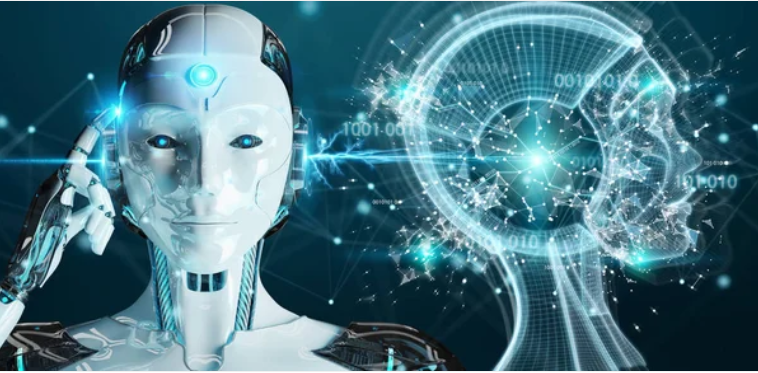
\includegraphics[width=8.49444in,height=4.14861in]{11-Actions Mécaniques/Cours/pandoc/media/image1.png}

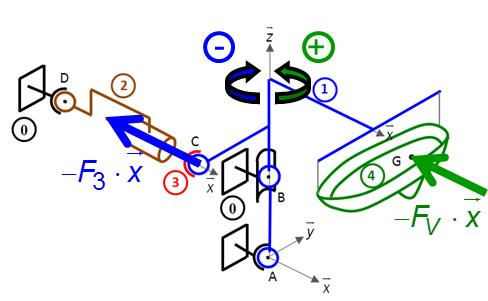
\includegraphics[width=2.77222in,height=2.48472in]{11-Actions Mécaniques/Cours/pandoc/media/image3.jpeg}

Cycle 6 : Analyser, Modéliser, Expérimenter et Résoudre les performances de systèmes de solide d'une chaîne d'énergie

\textbf{Détermination des actions mécaniques}

Thomas Lusseau

Lycée Robert Doisneau - ATS

Table des matières

\protect\hyperlink{introduction}{1. Introduction {[}8{]}(\#introduction)}

\protect\hyperlink{duxe9marche-de-ruxe9solution-pour-duxe9terminer-les-actions-muxe9caniques}{2. Démarche de résolution pour déterminer les Actions Mécaniques {[}8{]}(\#démarche-de-résolution-pour-déterminer-les-actions-mécaniques)}

\protect\hyperlink{duxe9marche-de-ruxe9solution}{2.1. Démarche de résolution {[}8{]}(\#démarche-de-résolution)}

\protect\hyperlink{repruxe9senter-le-systuxe8me-graphe-de-structure-et-schuxe9ma-darchitecture}{2.2. Représenter le système~: graphe de structure et schéma d'architecture {[}9{]}(\#représenter-le-système-graphe-de-structure-et-schéma-darchitecture)}

\protect\hyperlink{isoler-une-partie-du-systuxe8me}{2.3. Isoler une partie du système {[}10{]}(\#isoler-une-partie-du-système)}

\protect\hyperlink{duxe9marche-de-ruxe9solution-stratuxe9gie-disolement}{2.4. Démarche de résolution~: Stratégie d'isolement {[}11{]}(\#démarche-de-résolution-stratégie-disolement)}

\protect\hyperlink{recenser-les-actions-muxe9caniques}{2.5. Recenser les actions mécaniques {[}15{]}(\#recenser-les-actions-mécaniques)}

\protect\hyperlink{actions-muxe9caniques}{3. Actions mécaniques {[}16{]}(\#actions-mécaniques)}

\protect\hyperlink{duxe9finition}{3.1. Définition {[}16{]}(\#définition)}

\protect\hyperlink{torseurs-dam-particuliers-torseur-glisseur-torseur-couple}{3.2. Torseurs d'AM particuliers~: Torseur glisseur, Torseur couple {[}17{]}(\#torseurs-dam-particuliers-torseur-glisseur-torseur-couple)}

\protect\hyperlink{thuxe9oruxe8me-des-actions-ruxe9ciproques}{3.3. Théorème des actions réciproques {[}17{]}(\#théorème-des-actions-réciproques)}

\protect\hyperlink{cas-de-laction-muxe9canique-de-la-pesanteur}{3.4. Cas de l'action mécanique de la pesanteur {[}17{]}(\#cas-de-laction-mécanique-de-la-pesanteur)}

\protect\hyperlink{actions-muxe9caniques-particuliuxe8res-uxe0-connauxeetre}{3.5. Actions mécaniques particulières à connaître {[}19{]}(\#actions-mécaniques-particulières-à-connaître)}

\protect\hyperlink{actions-muxe9caniques-transmissibles-par-les-liaisons-usuelles}{3.6. Actions mécaniques transmissibles par les liaisons usuelles {[}21{]}(\#actions-mécaniques-transmissibles-par-les-liaisons-usuelles)}

\protect\hyperlink{cas-particulier-dun-probluxe8me-plan}{3.7. Cas particulier d'un problème plan {[}25{]}(\#cas-particulier-dun-problème-plan)}

\protect\hyperlink{etude-de-luxe9quilibre-dun-systuxe8me}{4. Etude de l'équilibre d'un système {[}26{]}(\#etude-de-léquilibre-dun-système)}

\protect\hyperlink{etude-de-luxe9quilibre-principe-de-la-statique}{4.1. Etude de l'équilibre~: Principe de la Statique {[}26{]}(\#etude-de-léquilibre-principe-de-la-statique)}

\protect\hyperlink{duxe9marche-de-ruxe9solution-dun-probluxe8me-pour-uxe9tudier-luxe9quilibre}{4.2. Démarche de résolution d'un problème pour étudier l'équilibre {[}27{]}(\#démarche-de-résolution-dun-problème-pour-étudier-léquilibre)}

\protect\hyperlink{conseils-pour-le-choix-du-point-de-ruxe9duction}{4.3. Conseils pour le choix du point de réduction {[}27{]}(\#conseils-pour-le-choix-du-point-de-réduction)}

\protect\hyperlink{inventaire-ou-bilan-des-actions-muxe9caniques-extuxe9rieurs-bame}{4.4. Inventaire (ou bilan) des actions mécaniques extérieurs (BAME) {[}27{]}(\#inventaire-ou-bilan-des-actions-mécaniques-extérieurs-bame)}

\protect\hyperlink{ensemble-isoluxe9-soumis-uniquement-uxe0-des-torseurs-glisseurs}{4.5. Ensemble isolé soumis uniquement à des torseurs glisseurs {[}28{]}(\#ensemble-isolé-soumis-uniquement-à-des-torseurs-glisseurs)}

\protect\hyperlink{synthuxe8se-de-la-duxe9marche-de-ruxe9solution-dun-probluxe8me-duxe9quilibre}{4.6. Synthèse de la démarche de résolution d'un problème d'équilibre {[}31{]}(\#synthèse-de-la-démarche-de-résolution-dun-problème-déquilibre)}

\protect\hyperlink{duxe9finir-une-action-muxe9canique-point-de-vue-local}{5. Définir une action mécanique~: Point de vue local {[}35{]}(\#définir-une-action-mécanique-point-de-vue-local)}

\protect\hyperlink{duxe9finir-une-action-muxe9canique-du-point-de-vue-local-au-point-de-vue-global}{5.1. Définir une action mécanique~: du point de vue local au point de vue global {[}35{]}(\#définir-une-action-mécanique-du-point-de-vue-local-au-point-de-vue-global)}

\protect\hyperlink{torseur-des-actions-muxe9caniques}{5.2. Torseur des actions mécaniques {[}36{]}(\#torseur-des-actions-mécaniques)}

\protect\hyperlink{prise-en-compte-du-phuxe9nomuxe8ne-de-frottement}{6. Prise en compte du phénomène de frottement {[}40{]}(\#prise-en-compte-du-phénomène-de-frottement)}

\protect\hyperlink{frottement-en-translation}{6.1. Frottement en translation {[}40{]}(\#frottement-en-translation)}

\protect\hyperlink{prise-en-compte-du-phuxe9nomuxe8ne-de-frottement-dans-une-liaison-pivot}{6.2. Prise en compte du phénomène de frottement dans une liaison pivot {[}45{]}(\#prise-en-compte-du-phénomène-de-frottement-dans-une-liaison-pivot)}

\protect\hyperlink{phuxe9nomuxe8ne-darc-boutement}{6.3. Phénomène d'arc-boutement {[}46{]}(\#phénomène-darc-boutement)}

\protect\hyperlink{moment-dune-force-et-bras-de-levier}{7. Moment d'une force et Bras de Levier {[}46{]}(\#moment-dune-force-et-bras-de-levier)}

\protect\hyperlink{masse-centre-dinertie}{8. Masse -- Centre d'inertie {[}50{]}(\#masse-centre-dinertie)}

\protect\hyperlink{masse}{8.1. Masse {[}50{]}(\#masse)}

\protect\hyperlink{centre-dinertie}{8.2. Centre d'inertie {[}50{]}(\#centre-dinertie)}

\protect\hyperlink{opuxe9rateur-dinertie---effets-dinertie}{9. Opérateur d'inertie - Effets d'inertie {[}53{]}(\#opérateur-dinertie---effets-dinertie)}

\protect\hyperlink{moment-dinertie}{9.1. Moment d'inertie {[}53{]}(\#moment-dinertie)}

\protect\hyperlink{produit-dinertie}{9.2. Produit d'inertie {[}54{]}(\#produit-dinertie)}

\protect\hyperlink{lopuxe9rateur-dinertie-la-matrice-dinertie-dun-solide-i0s}{9.3. L'opérateur d'inertie~: la matrice d'inertie~d'un solide {[}I\textsubscript{0}(S){]} {[}54{]}(\#lopérateur-dinertie-la-matrice-dinertie-dun-solide-i0s)}

\protect\hyperlink{symuxe9tries-matuxe9rielles}{9.4. Symétries matérielles {[}56{]}(\#symétries-matérielles)}

\protect\hyperlink{thuxe9oruxe8me-de-huygens-guxe9nuxe9ralisuxe9}{9.5. Théorème de Huygens généralisé {[}57{]}(\#théorème-de-huygens-généralisé)}

\protect\hyperlink{duxe9termination-de-la-matrice-dinertie-uxe0-partir-des-ruxe9sultats-classiques}{9.6. Détermination de la matrice d'inertie à partir des résultats classiques {[}59{]}(\#détermination-de-la-matrice-dinertie-à-partir-des-résultats-classiques)}

\protect\hyperlink{equilibrage-dynamique}{9.7. Equilibrage dynamique {[}63{]}(\#equilibrage-dynamique)}

\protect\hyperlink{le-thuxe9oruxe8me-de-luxe9nergie-cinuxe9tique-galiluxe9enne-ou-uxe9nergie-puissance}{10. Le théorème de l'énergie cinétique Galiléenne (ou énergie-puissance) {[}63{]}(\#le-théorème-de-lénergie-cinétique-galiléenne-ou-énergie-puissance)}

\protect\hyperlink{introduction-1}{10.1. Introduction {[}63{]}(\#introduction-1)}

\protect\hyperlink{thuxe9oruxe8me-de-luxe9nergie-cinuxe9tique-galiluxe9enne-ou-thuxe9oruxe8me-uxe9nergie-puissance}{10.2. Théorème de l'énergie cinétique Galiléenne (ou théorème énergie puissance) {[}63{]}(\#théorème-de-lénergie-cinétique-galiléenne-ou-théorème-énergie-puissance)}

\protect\hyperlink{duxe9marche-de-ruxe9solution-1}{10.3. Démarche de résolution {[}64{]}(\#démarche-de-résolution-1)}

\protect\hyperlink{torseur-cinuxe9tique}{10.4. Torseur cinétique {[}65{]}(\#torseur-cinétique)}

\protect\hyperlink{duxe9terminer-luxe9nergie-cinuxe9tique-dun-solide}{10.5. Déterminer l'énergie cinétique d'un solide {[}67{]}(\#déterminer-lénergie-cinétique-dun-solide)}

\protect\hyperlink{duxe9termination-du-moment-dinertie-uxe9quivalent-et-de-la-masse-uxe9quivalente}{10.6. Détermination du moment d'inertie équivalent et de la masse équivalente {[}69{]}(\#détermination-du-moment-dinertie-équivalent-et-de-la-masse-équivalente)}

\protect\hyperlink{notion-de-puissance-muxe9canique}{10.7. Notion de puissance mécanique {[}72{]}(\#notion-de-puissance-mécanique)}

\protect\hyperlink{puissance-extuxe9rieure}{10.8. Puissance extérieure {[}72{]}(\#puissance-extérieure)}

\protect\hyperlink{puissance-duxe9veloppuxe9e-par-les-actions-mutuelles-entre-deux-solides-pint}{10.9. Puissance développée par les actions mutuelles entre deux solides (P\textsubscript{int}) {[}72{]}(\#puissance-développée-par-les-actions-mutuelles-entre-deux-solides-pint)}

\protect\hyperlink{travail-uxe9nergie-potentielle-et-puissance}{10.10. Travail, énergie potentielle et puissance {[}75{]}(\#travail-énergie-potentielle-et-puissance)}

\protect\hyperlink{principe-fondamental-de-la-dynamique}{11. Principe Fondamental de la Dynamique {[}76{]}(\#principe-fondamental-de-la-dynamique)}

\protect\hyperlink{enoncuxe9-du-pfd}{11.1. Enoncé du PFD {[}76{]}(\#enoncé-du-pfd)}

\protect\hyperlink{torseur-dynamique}{11.2. Torseur Dynamique {[}77{]}(\#torseur-dynamique)}

\protect\hyperlink{cas-simplifiuxe9s}{11.3. Cas simplifiés {[}78{]}(\#cas-simplifiés)}

\protect\hyperlink{sources}{12. Sources {[}82{]}(\#sources)}

\protect\hyperlink{_Toc126746027}{13. Exercices du chapitre {[}83{]}(\#\_Toc126746027)}

\protect\hyperlink{equilibre}{14. EQUILIBRE {[}84{]}(\#equilibre)}

\protect\hyperlink{theoreme-de-lenergie-cinetique}{15. THEOREME DE L'ENERGIE CINETIQUE {[}94{]}(\#theoreme-de-lenergie-cinetique)}

\protect\hyperlink{pfd}{16. PFD {[}128{]}(\#pfd)}

Choisir et utiliser des démarches et des méthodes pour décrire et caractériser les actions mécaniques d'un système afin de prévoir son comportement et/ou de le dimensionner

Etude de l'équilibre

\textbf{Je connais~:}

\begin{longtable}[]{@{}
  >{\raggedright\arraybackslash}p{(\columnwidth - 2\tabcolsep) * \real{0.9028}}
  >{\raggedright\arraybackslash}p{(\columnwidth - 2\tabcolsep) * \real{0.0833}}@{}}
\toprule\noalign{}
\begin{minipage}[b]{\linewidth}\raggedright
\begin{itemize}
\tightlist
\item
  les différents types d'action mécanique~;
\end{itemize}
\end{minipage} & \begin{minipage}[b]{\linewidth}\raggedright
⃝
\end{minipage} \\
\midrule\noalign{}
\endhead
\bottomrule\noalign{}
\endlastfoot
\begin{minipage}[t]{\linewidth}\raggedright
\begin{itemize}
\tightlist
\item
  les torseurs particuliers~: torseur couple et torseur glisseur~;
\end{itemize}
\end{minipage} & ⃝ \\
\begin{minipage}[t]{\linewidth}\raggedright
\begin{itemize}
\tightlist
\item
  le théorème des actions réciproques ;
\end{itemize}
\end{minipage} & ⃝ \\
\begin{minipage}[t]{\linewidth}\raggedright
\begin{itemize}
\tightlist
\item
  les notions de frottement et d'adhérence~et les lois de Coulomb;
\end{itemize}
\end{minipage} & ⃝ \\
\begin{minipage}[t]{\linewidth}\raggedright
\begin{itemize}
\tightlist
\item
  la notion d'arc-boutement;
\end{itemize}
\end{minipage} & ⃝ \\
\begin{minipage}[t]{\linewidth}\raggedright
\begin{itemize}
\tightlist
\item
  les torseurs d'actions mécaniques transmissibles par les liaisons usuelles~;
\end{itemize}
\end{minipage} & ⃝ \\
\begin{minipage}[t]{\linewidth}\raggedright
\begin{itemize}
\tightlist
\item
  le principe fondamental de la statique~;
\end{itemize}
\end{minipage} & ⃝ \\
\begin{minipage}[t]{\linewidth}\raggedright
\begin{itemize}
\tightlist
\item
  le théorème de la résultante statique et le théorème du moment statique
\end{itemize}
\end{minipage} & ⃝ \\
\begin{minipage}[t]{\linewidth}\raggedright
\begin{itemize}
\tightlist
\item
  les résultats pour les solides soumis au maximum à trois actions mécaniques modélisables par des torseurs glisseurs.
\end{itemize}
\end{minipage} & ⃝ \\
\end{longtable}

\textbf{Je sais~:}

\begin{longtable}[]{@{}
  >{\raggedright\arraybackslash}p{(\columnwidth - 2\tabcolsep) * \real{0.9028}}
  >{\raggedright\arraybackslash}p{(\columnwidth - 2\tabcolsep) * \real{0.0833}}@{}}
\toprule\noalign{}
\begin{minipage}[b]{\linewidth}\raggedright
\begin{itemize}
\tightlist
\item
  modéliser une action mécanique au niveau local~et au \textgreater{} niveau global à l'aide d'un torseur~;
\end{itemize}
\end{minipage} & \begin{minipage}[b]{\linewidth}\raggedright
⃝
\end{minipage} \\
\midrule\noalign{}
\endhead
\bottomrule\noalign{}
\endlastfoot
\begin{minipage}[t]{\linewidth}\raggedright
\begin{itemize}
\tightlist
\item
  modéliser au niveau local et au niveau global l'action \textgreater{} mécanique de contact dans le cas d'une tendance au \textgreater{} glissement avec adhérence~ou d'un glissement avec \textgreater{} frottement;
\end{itemize}
\end{minipage} & ⃝ \\
\begin{minipage}[t]{\linewidth}\raggedright
\begin{itemize}
\tightlist
\item
  faire le bilan des actions mécaniques extérieures à un \textgreater{} ensemble isolé;
\end{itemize}
\end{minipage} & ⃝ \\
\begin{minipage}[t]{\linewidth}\raggedright
\begin{itemize}
\tightlist
\item
  simplifier un torseur d'actions mécaniques dans le cas \textgreater{} d'un problème plan;
\end{itemize}
\end{minipage} & ⃝ \\
\begin{minipage}[t]{\linewidth}\raggedright
\begin{itemize}
\tightlist
\item
  utiliser une méthode de résolution adaptée à une \textgreater{} problématique.
\end{itemize}
\end{minipage} & ⃝ \\
\end{longtable}

Masse et Inertie

\textbf{Je connais~:}

\begin{longtable}[]{@{}
  >{\raggedright\arraybackslash}p{(\columnwidth - 2\tabcolsep) * \real{0.9028}}
  >{\raggedright\arraybackslash}p{(\columnwidth - 2\tabcolsep) * \real{0.0833}}@{}}
\toprule\noalign{}
\begin{minipage}[b]{\linewidth}\raggedright
\begin{itemize}
\tightlist
\item
  La définition mathématique de la masse d'un solide~;
\end{itemize}
\end{minipage} & \begin{minipage}[b]{\linewidth}\raggedright
⃝
\end{minipage} \\
\midrule\noalign{}
\endhead
\bottomrule\noalign{}
\endlastfoot
\begin{minipage}[t]{\linewidth}\raggedright
\begin{itemize}
\tightlist
\item
  La relation permettant de trouver la position du centre d'inertie d'un ensemble de solides~;
\end{itemize}
\end{minipage} & ⃝ \\
\begin{minipage}[t]{\linewidth}\raggedright
\begin{itemize}
\tightlist
\item
  La différence entre moment d'inertie et produit d'inertie ;
\end{itemize}
\end{minipage} & ⃝ \\
\begin{minipage}[t]{\linewidth}\raggedright
\begin{itemize}
\tightlist
\item
  La définition de la matrice d'inertie et ses composantes;
\end{itemize}
\end{minipage} & ⃝ \\
\end{longtable}

\textbf{Je sais~:}

\begin{longtable}[]{@{}
  >{\raggedright\arraybackslash}p{(\columnwidth - 2\tabcolsep) * \real{0.9028}}
  >{\raggedright\arraybackslash}p{(\columnwidth - 2\tabcolsep) * \real{0.0833}}@{}}
\toprule\noalign{}
\begin{minipage}[b]{\linewidth}\raggedright
\begin{itemize}
\tightlist
\item
  déterminer la masse d'un solide homogène~;
\end{itemize}
\end{minipage} & \begin{minipage}[b]{\linewidth}\raggedright
⃝
\end{minipage} \\
\midrule\noalign{}
\endhead
\bottomrule\noalign{}
\endlastfoot
\begin{minipage}[t]{\linewidth}\raggedright
\begin{itemize}
\tightlist
\item
  déterminer la position du centre d'inertie d'un solide \textgreater{} élémentaire et la position du centre d'inertie d'un \textgreater{} ensemble de solides;
\end{itemize}
\end{minipage} & ⃝ \\
\begin{minipage}[t]{\linewidth}\raggedright
\begin{itemize}
\tightlist
\item
  déterminer la forme de la matrice d'inertie d'un solide à \textgreater{} partir de sa géométrie et des symétries matérielles;
\end{itemize}
\end{minipage} & ⃝ \\
\begin{minipage}[t]{\linewidth}\raggedright
\begin{itemize}
\tightlist
\item
  déplacer la matrice d'inertie avec le théorème de \textgreater{} Huygens;
\end{itemize}
\end{minipage} & ⃝ \\
\begin{minipage}[t]{\linewidth}\raggedright
\begin{itemize}
\tightlist
\item
  déterminer la résultante cinétique et le moment cinétique.
\end{itemize}
\end{minipage} & ⃝ \\
\end{longtable}

Théorème de l'énergie cinétique

\textbf{Je connais~:}

\begin{longtable}[]{@{}
  >{\raggedright\arraybackslash}p{(\columnwidth - 2\tabcolsep) * \real{0.9028}}
  >{\raggedright\arraybackslash}p{(\columnwidth - 2\tabcolsep) * \real{0.0833}}@{}}
\toprule\noalign{}
\begin{minipage}[b]{\linewidth}\raggedright
\begin{itemize}
\tightlist
\item
  La définition de l'énergie cinétique sous forme de torseurs~;
\end{itemize}
\end{minipage} & \begin{minipage}[b]{\linewidth}\raggedright
⃝
\end{minipage} \\
\midrule\noalign{}
\endhead
\bottomrule\noalign{}
\endlastfoot
\begin{minipage}[t]{\linewidth}\raggedright
\begin{itemize}
\tightlist
\item
  L'expression des énergies cinétiques pour un mouvement de translation et pour un mouvement de rotation~;
\end{itemize}
\end{minipage} & ⃝ \\
\begin{minipage}[t]{\linewidth}\raggedright
\begin{itemize}
\tightlist
\item
  La définition de puissance d'une action mécanique sous forme de torseurs ;
\end{itemize}
\end{minipage} & ⃝ \\
\begin{minipage}[t]{\linewidth}\raggedright
\begin{itemize}
\tightlist
\item
  La définition de puissance des inter-efforts;
\end{itemize}
\end{minipage} & ⃝ \\
\begin{minipage}[t]{\linewidth}\raggedright
\begin{itemize}
\tightlist
\item
  Les cas particuliers pour les calculs de puissance;
\end{itemize}
\end{minipage} & ⃝ \\
\begin{minipage}[t]{\linewidth}\raggedright
\begin{itemize}
\tightlist
\item
  Le théorème général de l'énergie cinétique~;
\end{itemize}
\end{minipage} & ⃝ \\
\begin{minipage}[t]{\linewidth}\raggedright
\begin{itemize}
\tightlist
\item
  L'expression des puissances «~perdues~» à partir des rendements~;
\end{itemize}
\end{minipage} & ⃝ \\
\end{longtable}

\textbf{Je sais~:}

\begin{longtable}[]{@{}
  >{\raggedright\arraybackslash}p{(\columnwidth - 2\tabcolsep) * \real{0.9028}}
  >{\raggedright\arraybackslash}p{(\columnwidth - 2\tabcolsep) * \real{0.0833}}@{}}
\toprule\noalign{}
\begin{minipage}[b]{\linewidth}\raggedright
\begin{itemize}
\tightlist
\item
  déterminer l'énergie cinétique d'un solide ou d'un \textgreater{} ensemble de solides~;
\end{itemize}
\end{minipage} & \begin{minipage}[b]{\linewidth}\raggedright
⃝
\end{minipage} \\
\midrule\noalign{}
\endhead
\bottomrule\noalign{}
\endlastfoot
\begin{minipage}[t]{\linewidth}\raggedright
\begin{itemize}
\tightlist
\item
  déterminer la puissance développée par une action \textgreater{} mécanique;
\end{itemize}
\end{minipage} & ⃝ \\
\begin{minipage}[t]{\linewidth}\raggedright
\begin{itemize}
\tightlist
\item
  déterminer un moment d'inertie équivalent;
\end{itemize}
\end{minipage} & ⃝ \\
\begin{minipage}[t]{\linewidth}\raggedright
\begin{itemize}
\tightlist
\item
  appliquer le TGEC pour déterminer une équation de \textgreater{} mouvement;
\end{itemize}
\end{minipage} & ⃝ \\
\end{longtable}

Principe Fondamental de la Dynamique

\textbf{Je connais~:}

\begin{longtable}[]{@{}
  >{\raggedright\arraybackslash}p{(\columnwidth - 2\tabcolsep) * \real{0.9028}}
  >{\raggedright\arraybackslash}p{(\columnwidth - 2\tabcolsep) * \real{0.0833}}@{}}
\toprule\noalign{}
\begin{minipage}[b]{\linewidth}\raggedright
\begin{itemize}
\tightlist
\item
  La définition du torseur dynamique~;
\end{itemize}
\end{minipage} & \begin{minipage}[b]{\linewidth}\raggedright
⃝
\end{minipage} \\
\midrule\noalign{}
\endhead
\bottomrule\noalign{}
\endlastfoot
\begin{minipage}[t]{\linewidth}\raggedright
\begin{itemize}
\tightlist
\item
  Les expressions de la résultante dynamique et du moment dynamique ainsi que les cas particuliers (point fixe, centre d'inertie)~;
\end{itemize}
\end{minipage} & ⃝ \\
\begin{minipage}[t]{\linewidth}\raggedright
\begin{itemize}
\tightlist
\item
  Le PFD sous forme torsorielle et vectorielle ;
\end{itemize}
\end{minipage} & ⃝ \\
\end{longtable}

\textbf{Je sais~:}

\begin{longtable}[]{@{}
  >{\raggedright\arraybackslash}p{(\columnwidth - 2\tabcolsep) * \real{0.9028}}
  >{\raggedright\arraybackslash}p{(\columnwidth - 2\tabcolsep) * \real{0.0833}}@{}}
\toprule\noalign{}
\begin{minipage}[b]{\linewidth}\raggedright
\begin{itemize}
\tightlist
\item
  déterminer le torseur dynamique~d'un solide par rapport à \textgreater{} un référentiel galiléen;
\end{itemize}
\end{minipage} & \begin{minipage}[b]{\linewidth}\raggedright
⃝
\end{minipage} \\
\midrule\noalign{}
\endhead
\bottomrule\noalign{}
\endlastfoot
\begin{minipage}[t]{\linewidth}\raggedright
\begin{itemize}
\tightlist
\item
  appliquer le PFD à un ensemble de solides.
\end{itemize}
\end{minipage} & ⃝ \\
\end{longtable}

\hypertarget{introduction}{%
\subsection{Introduction}\label{introduction}}

On a vu précédement que l'on pouvait, à l'aide d'une simulation «~manuelle» ou assistée par ordinateur, prévoir le comportement cinématique des systèmes.

Mais cela ne suffit pas pour concevoir un système ou vérifier qu'il répond bien aux attentes de ses utilisateurs. Il faut aussi s'intéresser aux \textbf{actions mécaniques} auxquelles les constituants de ce système sont soumis afin de \textbf{dimensionner les pièces qui le constituent, prévoir leurs déformations ou bien déterminer certaines caractéristiques des actionneurs comme le couple moteur.}

C'est l'application de différents principes qui, après avoir identifié et caractérisé les différentes actions mécaniques connues et recherchées, permettent d'étudier la relation de cause à effet entre les performances d'un système et les actions mécaniques en présence.

\hypertarget{duxe9marche-de-ruxe9solution-pour-duxe9terminer-les-actions-muxe9caniques}{%
\subsection{Démarche de résolution pour déterminer les Actions Mécaniques}\label{duxe9marche-de-ruxe9solution-pour-duxe9terminer-les-actions-muxe9caniques}}

\hypertarget{duxe9marche-de-ruxe9solution}{%
\subsubsection{Démarche de résolution}\label{duxe9marche-de-ruxe9solution}}

La démarche utilisée pour un résoudre une problématique liée à la détermination d'actions mécaniques sur un système en équilibre, peut se résumer à~:

\hypertarget{repruxe9senter-le-systuxe8me-graphe-de-structure-et-schuxe9ma-darchitecture}{%
\subsubsection{Représenter le système~: graphe de structure et schéma d'architecture}\label{repruxe9senter-le-systuxe8me-graphe-de-structure-et-schuxe9ma-darchitecture}}

Un des objectifs, lors de l'étude du comportement statique d'un système, peut être de valider le dimensionnement des solutions techniques adoptées par le concepteur du système pour réaliser les liaisons.

Dans ce cas, le schéma cinématique minimal construit à partir du graphe des liaisons, ne suffit plus.

On utilise alors des outils de représentation qui collent plus à la réalité technologique du système et qui font apparaître plus clairement les différents constituants et les actions mécaniques mises en jeu.

Sur le graphe de structure et le schéma architectural figurent~:

\begin{itemize}
\item
  toutes \textbf{\emph{les liaisons élémentaires}} sans les regrouper en liaisons équivalentes~;
\item
  \textbf{\emph{les actions mécaniques extérieures et intérieures au système}} (de contact ou à distance)~: \emph{couple moteur, pression d'un fluide, action d'un ressort, action de la pesanteur\ldots{}}
\end{itemize}

Ces outils de représentation ne sont pas normalisés. L'objectif est de faire apparaitre toutes les informations qui vont ensuite faciliter le bilan des actions mécaniques lors de l'isolement de solides ou de groupes de solides~!

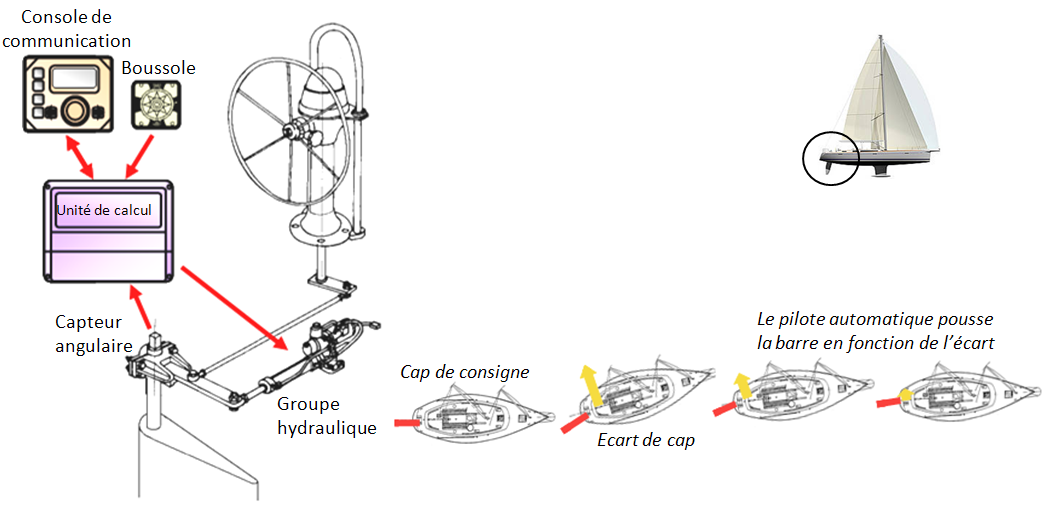
\includegraphics[width=4.97917in,height=2.44931in]{11-Actions Mécaniques/Cours/pandoc/media/image5.png}\textbf{\emph{\ul{Exemple~:}}}

\emph{L'ensemble gouvernail barre franche 1 est en liaison pivot d'axe (A,}\(\overrightarrow{z}\)\emph{) par rapport à la coque du bateau 0. Lorsque le pilotage est automatique, l'ensemble 1 est actionné par un vérin (2+3).}

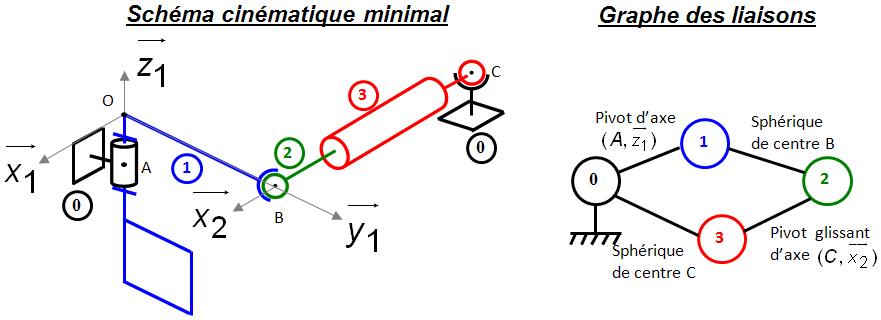
\includegraphics[width=5.23264in,height=1.90694in]{11-Actions Mécaniques/Cours/pandoc/media/image6.png}

La liaison pivot d'axe (A,\(\overrightarrow{z}\)) entre 1 et 0 est un modèle adapté pour une étude du comportement cinématique du système car Il traduit le mouvement de 1/0 observé sur le système réel.

Dans le cas d'une étude du comportement statique dont l'objectif serait de dimensionner les solutions techniques qui permettent ce mouvement, il faut tenir compte des composants technologiques utilisés. En l'occurrence on utilise deux roulements à billes à contact radial ayant pour centres de poussée respectifs les points A\textsubscript{1} et A\textsubscript{2} éloignés d'une distance L. On choisit donc de modéliser ces composants technologiques par une liaison sphérique rotule de centre A\textsubscript{1} et une liaison sphère-cylindre de centre A\textsubscript{2} et de direction \(\overrightarrow{z}\). Cela permettra de déterminer plus facilement les actions mécaniques exercées sur chacun des roulements à billes.

On ajoute aussi, sur le schéma cinématique et le graphe des liaisons, des informations sur les actions mécaniques extérieures et intérieures au système :

\begin{itemize}
\item
  l'eau exerce une action mécanique sur le gouvernail modélisée globalement par une résultante \(\overset{\rightarrow}{F_{eau \rightarrow 1}} = - F.\overrightarrow{x}\) au point P~;
\item
  à l'intérieur du vérin, le fluide sous pression exerce une action mécanique sur le corps du vérin 3 ainsi que sur la tige du vérin 2~;
\item
  seuls les ensembles 0 et 1 sont soumis à l'action mécanique de la pesanteur \(\overrightarrow{g}\) (Hypothèse~: on néglige cette AM sur les solides 2 et 3).
\end{itemize}

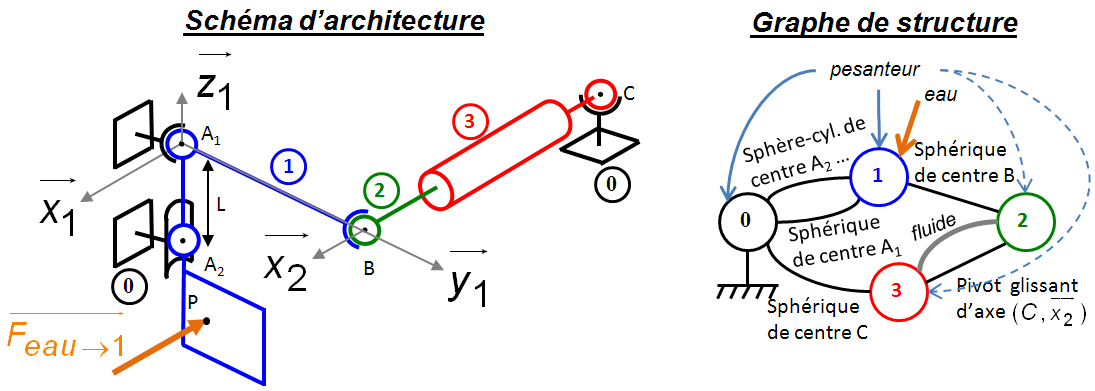
\includegraphics[width=5.5in,height=1.95347in]{11-Actions Mécaniques/Cours/pandoc/media/image7.png}

\hypertarget{isoler-une-partie-du-systuxe8me}{%
\subsubsection{Isoler une partie du système}\label{isoler-une-partie-du-systuxe8me}}

Isoler un solide ou un ensemble de solides revient à définir une frontière fictive qui englobe cet ensemble isolé et définir ainsi~:

\begin{itemize}
\item
  \textbf{\emph{un milieu intérieur}} (qui est dans la frontière), noté \(\Sigma\)~;
\item
  \textbf{\emph{un milieu extérieur}} (qui est en dehors de la frontière) noté \(\overline{\Sigma}\)~.
\end{itemize}

Souvent on représente cet isolement avec une frontière. Chaque fois qu'une action mécanique (AM) coupe cette frontière, on parlera d'action mécanique extérieure.

\textbf{Quand on isole un solide (ou un ensemble de solides) le numéro du (ou des) solide(s) isolé(s) se trouve toujours à droite.}

\begin{longtable}[]{@{}
  >{\raggedright\arraybackslash}p{(\columnwidth - 2\tabcolsep) * \real{0.1111}}
  >{\raggedright\arraybackslash}p{(\columnwidth - 2\tabcolsep) * \real{0.8750}}@{}}
\toprule\noalign{}
\begin{minipage}[b]{\linewidth}\raggedright
\begin{quote}
\includegraphics{1 1-Act ions Mécan iques /Cour s/pan doc/m edia/ image 8.png}\{wid th=``0 .6262 69685 03937 01in''

heigh t=``0. 65083 33333 33333 4in''\}
\end{quote}
\end{minipage} & \begin{minipage}[b]{\linewidth}\raggedright
\textbf{Pilote de bateau}

\textbf{Isoler l'ensemble} \(\mathbf{\Sigma = 2 + 3}\)


\includegraphics[width=5.89514in,height=1.84861in]{11-Actions Mécanique s/Cours/pandoc/media/image9.png}

Bilan des Actions Mécaniques (AM) extérieures à \(\Sigma = 2 + 3\)~:

\begin{itemize}
\item
  AM de \(0 \rightarrow 3\) ;
\item
  AM de \(1 \rightarrow 2\) ~;
\item
  AM de \(pes \rightarrow 3\)~;
\item
  AM de \(pes \rightarrow 2\);
\end{itemize}
\end{minipage} \\
\midrule\noalign{}
\endhead
\bottomrule\noalign{}
\endlastfoot
& \\
\end{longtable}

\hypertarget{duxe9marche-de-ruxe9solution-stratuxe9gie-disolement}{%
\subsubsection{Démarche de résolution~: Stratégie d'isolement}\label{duxe9marche-de-ruxe9solution-stratuxe9gie-disolement}}

Les systèmes mécaniques sont souvent conçus de telle façon à avoir une loi entrée-sortie en effort : un effecteur est soumis à un effort qui se transmet de solides en solides jusqu'à l'actionneur (souvent un moteur ou un vérin), qui compense cet effort. Il est parfois nécessaire de faire plusieurs isolements, à des sous-systèmes différents, afin de déterminer les AM recherchées. Deux stratégies sont possibles :

\begin{itemize}
\item
  Le calcul complet de toutes les AM possibles entre les solides, en isolant chacun des solides à l'exception du bâti. Ceci amène à 6 x (nombre de solides -- 1) équations pour un problème 3D. C'est le calcul que fait généralement un logiciel non optimisé.
\item
  L'application de \textbf{certaines équations} (parfois une seule) uniquement à certains sous-systèmes judicieusement choisis afin d'obtenir les efforts inconnus désirés avec le moins de calculs possibles.
\end{itemize}

Remarque : \textbf{On n'isole jamais le bâti} ou un système comprenant le bâti, car le bâti est relié par liaison complète à un « support », et cela fait 6 inconnues statiques qui empêchent la résolution des autres inconnues recherchées.

Grâce au graphe de structure, il faut essayer de trouver par quels systèmes passer pour aller des données connues jusqu'à celle recherchée, en un minimum d'isolements et en un minimum d'équations. Un isolement permet de trouver des relations entre les différentes AM extérieures à l'ensemble isolé.

\begin{enumerate}
\def\labelenumi{\arabic{enumi}.}
\item
  Il faut commencer par rechercher les \textbf{systèmes soumis à 2 AM de type résultantes}, car on peut immédiatement en déduire la droite support de ces forces (et du coup éliminer des inconnues - une inconnue statique après isolement)
\item
  Déterminer le nombre d'inconnues statiques de liaisons pour chaque isolement (elles doivent être inférieures ou égales à 6)
\item
  Déterminer le «~chemin~» pour aller des AM connues aux AM à déterminer.
\end{enumerate}

\hypertarget{rappel-sur-les-inconnues-de-liaisons}{%
\subparagraph*{Rappel sur les inconnues de liaisons}\label{rappel-sur-les-inconnues-de-liaisons}}
\addcontentsline{toc}{subparagraph}{Rappel sur les inconnues de liaisons}

\begin{longtable}[]{@{}
  >{\raggedright\arraybackslash}p{(\columnwidth - 4\tabcolsep) * \real{0.1467}}
  >{\raggedright\arraybackslash}p{(\columnwidth - 4\tabcolsep) * \real{0.1733}}
  >{\raggedright\arraybackslash}p{(\columnwidth - 4\tabcolsep) * \real{0.6533}}@{}}
\toprule\noalign{}
\begin{minipage}[b]{\linewidth}\raggedright
Ic
\end{minipage} & \begin{minipage}[b]{\linewidth}\raggedright
Is
\end{minipage} & \begin{minipage}[b]{\linewidth}\raggedright
Liaisons
\end{minipage} \\
\midrule\noalign{}
\endhead
\bottomrule\noalign{}
\endlastfoot
1 & 5 & Pivot, glissière, hélicoïdale \\
2 & 4 & Pivot glissant, sphérique à doigt \\
3 & 3 & Appui-plan, sphérique \\
4 & 2 & Cylindre-plan, sphère-cylindre \\
5 & 1 & Sphère-plan \\
\end{longtable}

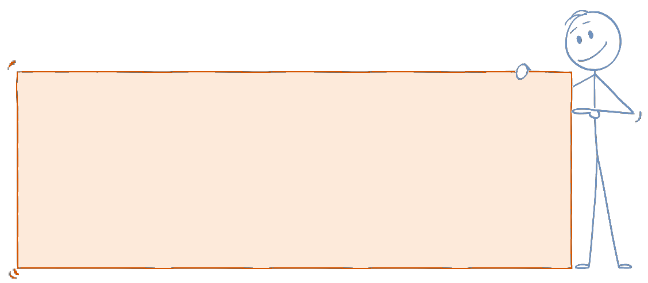
\includegraphics[width=2.96875in,height=1.28723in]{11-Actions Mécaniques/Cours/pandoc/media/image10.png}


\includegraphics[width=0.74722in,height=0.59167in]{11-Actions Mécaniques/Cours/pandoc/media/image12.png}Pour une liaison hélicoïdale, il n'y a qu'une seule inconnue cinématique indépendante puisque la translation est liée à la rotation par le pas de la vis.

\begin{longtable}[]{@{}
  >{\raggedright\arraybackslash}p{(\columnwidth - 2\tabcolsep) * \real{0.1111}}
  >{\raggedright\arraybackslash}p{(\columnwidth - 2\tabcolsep) * \real{0.8750}}@{}}
\toprule\noalign{}
\begin{minipage}[b]{\linewidth}\raggedright
\begin{quote}
\includegraphics{1 1-Act ions Mécan iques /Cour s/pan doc/m edia/ image 8.png}\{wid th=``0 .6262 69685 03937 01in''

heigh t=``0. 65083 33333 33333 4in''\}
\end{quote}
\end{minipage} & \begin{minipage}[b]{\linewidth}\raggedright
\textbf{Grue de port}

\textbf{Donner une stratégie d'isolement pour déterminer l'effort du vérin sur le bras 2} \(\over rightarrow{\mathbf{R}_{\mathbf{1}\mathbf{b \rightarrow 2}}}\) \textbf{afin de maintenir la grue en équilibre par rapport à l'effort de pesanteur.}


\includegraphics[width=2.4in,height=\textheight]{11-Acti ons Mécaniques/Cours/pandoc/media/image13.png}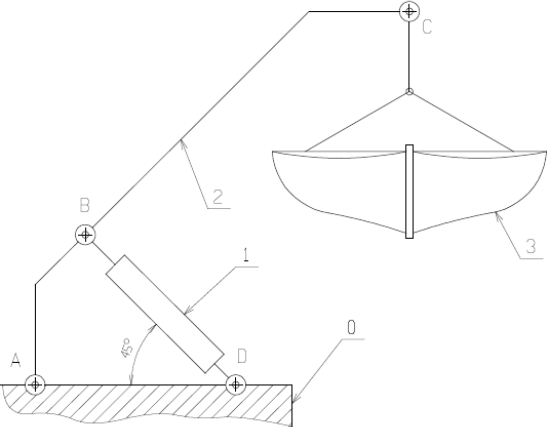
\includegraphics{11-Actions Mécaniques/Cours/pandoc/media/image15.png}

\begin{longtable}[]{@{}
  >{\raggedright\arraybackslash}p{(\columnwidth - 2\tabcolsep) * \real{0.3889}}
  >{\raggedright\arraybackslash}p{(\columnwidth - 2\tabcolsep) * \real{0.4028}}@{}}
\toprule\noalign{}
\begin{minipage}[b]{\linewidth}\raggedright
\textbf{Isolement 1}
\end{minipage} & \begin{minipage}[b]{\linewidth}\raggedright
\textbf{Isolement 2}
\end{minipage} \\
\midrule\noalign{}
\endhead
\bottomrule\noalign{}
\endlastfoot

\includegraphics{11-Acti ons Mécaniques/Cours/pand oc/media/image13.png}\{wid th=``1.6833333333333333in'' heig ht=``1.617577646544182in''\}

\(\Sigma = 1a + 1b\)

10 inconnues statiques (réduites à 2 car deux AM de type glisseur)

Cet isolement est soumis à deux AM de type glisseur et permet de diminuer le nombre d'inconnues statiques & 
\includegraphics{11-A ctions Mécaniques/Cours/pa ndoc/media/image13.png}\{wi dth=``1.6833333333333333in'' hei ght=``1.617577646544182in''\}

\(\Sigma = 2\)

5+1 = 6 inconnues statiques

Cet isolement permet d'avoir une relation entre l'AM \(\mathbf{pe s} \rightarrow \mathbf{2}\) et \(\mathbf{1 b} \rightarrow \mathbf{2}\) \\
\end{longtable}
\end{minipage} \\
\midrule\noalign{}
\endhead
\bottomrule\noalign{}
\endlastfoot
& \\
\end{longtable}

\begin{longtable}[]{@{}
  >{\raggedright\arraybackslash}p{(\columnwidth - 2\tabcolsep) * \real{0.1111}}
  >{\raggedright\arraybackslash}p{(\columnwidth - 2\tabcolsep) * \real{0.8750}}@{}}
\toprule\noalign{}
\begin{minipage}[b]{\linewidth}\raggedright
\begin{quote}
\includegraphics{1 1-Act ions Mécan iques /Cour s/pan doc/m edia/ image 8.png}\{wid th=``0 .6262 69685 03937 01in''

heigh t=``0. 65083 33333 33333 4in''\}
\end{quote}
\end{minipage} & \begin{minipage}[b]{\linewidth}\raggedright
\textbf{Pilote de bateau}


\includegraphics[width=3.44167in,height=1.84861in]{11-Actions Mécanique s/Cours/pandoc/media/image9.png}
\includegraphics[width=2.39167in,height=1.85094in]{11-Actions Mécaniques/C ours/pandoc/media/image16.jpeg}

\textbf{Déterminer la force délivrée par le vérin} \({\overrightarrow{\mathbf{F}}}_{\mathbf{v}}\) \textbf{en fonction de la force de l'eau sur le gouvernail} \({\overr ightarrow{\mathbf{F}}}_{\mathbf{eau}\mathbf{\rightarrow 1}}\)


\includegraphics[width=2.39167in,height=1.85069in]{11-Actions Mécaniques/C ours/pandoc/media/image16.jpeg}
\includegraphics[width=2.39167in,height=1.85094in]{11-Actions Mécaniques/C ours/pandoc/media/image16.jpeg}
\end{minipage} \\
\midrule\noalign{}
\endhead
\bottomrule\noalign{}
\endlastfoot
& \\
\end{longtable}

\begin{longtable}[]{@{}
  >{\raggedright\arraybackslash}p{(\columnwidth - 2\tabcolsep) * \real{0.1111}}
  >{\raggedright\arraybackslash}p{(\columnwidth - 2\tabcolsep) * \real{0.8750}}@{}}
\toprule\noalign{}
\begin{minipage}[b]{\linewidth}\raggedright
\begin{quote}
\includegraphics{1 1-Act ions Mécan iques /Cour s/pan doc/m edia/ image 8.png}\{wid th=``0 .6262 69685 03937 01in''

heigh t=``0. 65083 33333 33333 4in''\}
\end{quote}
\end{minipage} & \begin{minipage}[b]{\linewidth}\raggedright

\includegraphics[width=2.5in,height=1.925in]{11-Actio ns Mécaniques/Cours/pandoc/media/image17.jpeg}\textbf{Poussoir et coulisseau}

On associe les repères~:

\begin{quote}
- \(R_{0}(O,\overset{\rightarrow}{x_{0}} ,\overset{\rightarrow}{y_{0}},\overset{\rightarrow}{z_{0}})\) au bâti 0, tel que

\(\overset{\rightarrow}{OB} = b.\overset{\rightarrow}{x_{0}}\)

- \(R_{1}(O,\overset{\rightarrow}{x_{1}} ,\overset{\rightarrow}{y_{1}},\overset{\rightarrow}{z_{1}})\) au poussoir 1, tels que \(\over set{\rightarrow}{BA} = \lambda.\overset{\rightarrow}{y_{0}}\) et \(\alpha = (\overset{\rightarrow}{x_{0}},\overset{\rightarrow}{x_{1}})\)
\end{quote}

Un système non représenté assure le maintien du contact du coulisseau 2 avec le poussoir 1 au point A.

Le poussoir 1 est soumis au couple moteur \(C_{m}\) et le piston 2 à l'action 
\includegraphics{11-Actions Mécaniques/Cours/pandoc/media/image18.wmf} de pression du fluide.

On suppose le problème plan, les liaisons sans frottement et on néglige les effets d'inertie et de la pesanteur.

\textbf{L'objectif de l'étude est de déterminer une relation entre F et} \(\mathbf{C}_{\mathbf{m}}\) \textbf{lorsque le système est en équilibre.}

\textbf{Donner une stratégie d'isolement pour déterminer une relation entre le couple moteur} \(\mathbf{C}_{\mathbf{m}}\) \textbf{et l'effort} \(\mathbf{F}\)\textbf{.}
\end{minipage} \\
\midrule\noalign{}
\endhead
\bottomrule\noalign{}
\endlastfoot
& \\
\end{longtable}

\hypertarget{recenser-les-actions-muxe9caniques}{%
\subsubsection{Recenser les actions mécaniques}\label{recenser-les-actions-muxe9caniques}}

On définit~:

\begin{itemize}
\item
  des \textbf{actions mécaniques extérieures} qui correspondent à toutes \textgreater{} les actions mécaniques exercées par le milieu extérieur \textgreater{} \(\overline{\Sigma}\) (solide, fluide, ressort, pesanteur, \ldots) et \textgreater{} qui agissent \textbf{SUR} un des éléments du milieu intérieur \(\Sigma\).
\item
  des \textbf{actions mécaniques intérieures} qui correspondent à toutes \textgreater{} les actions mécaniques exercées par un élément (solide, fluide, \textgreater{} ressort, \ldots) appartenant au milieu intérieur \(\Sigma\) et qui agit \textgreater{} sur un autre élément du milieu intérieur \(\Sigma\).
\end{itemize}

Pour \textbf{\emph{recenser les actions mécaniques extérieures}}, on utilise \textbf{\emph{le graphe des structures}} sur lequel on vient directement \textbf{\emph{entourer l'ensemble isolé}}.

Chaque trait coupé par notre frontière d'étude correspond à une action mécanique extérieure que l'on décrit littéralement~: AM de 
\includegraphics{11-Actions Mécaniques/Cours/pandoc/media/image19.wmf} (\(i \in \overline{\Sigma}\) et \(j \in \Sigma\))

Chacune de ces actions mécaniques est ensuite modélisée à l'aide d'un torseur d'action mécanique~: \emph{\hfill\break
}\[\left\{ T_{i \rightarrow j} \right\} = \begin{Bmatrix}
\overrightarrow{R_{i \rightarrow j}} \\
\overrightarrow{M_{A,i \rightarrow j}}
\end{Bmatrix}_{A}\]

Lors de cette étape, on s'attachera à vérifier la présence ou non \textbf{\emph{d'hypothèses couramment utilisées~}}:

\begin{itemize}
\item
  \textbf{\emph{action de la pesanteur négligeable}} (lorsque la norme du poids des pièces est négligeable devant l'intensité des autres actions mécaniques)~;
\item
  \textbf{\emph{liaisons parfaites}}.
\end{itemize}

La somme de ces torseurs forme le torseur des actions mécaniques extérieures à 
\includegraphics{11-Actions Mécaniques/Cours/pandoc/media/image20.wmf}~:


\includegraphics{11-Actions Mécaniques/Cours/pandoc/media/image21.wmf} \emph{n est le nombre d'actions mécaniques extérieures}

\begin{longtable}[]{@{}
  >{\raggedright\arraybackslash}p{(\columnwidth - 2\tabcolsep) * \real{0.1111}}
  >{\raggedright\arraybackslash}p{(\columnwidth - 2\tabcolsep) * \real{0.8750}}@{}}
\toprule\noalign{}
\begin{minipage}[b]{\linewidth}\raggedright
\begin{quote}
\includegraphics{1 1-Act ions Mécan iques /Cour s/pan doc/m edia/ image 8.png}\{wid th=``0 .6262 69685 03937 01in''

heigh t=``0. 65083 33333 33333 4in''\}
\end{quote}
\end{minipage} & \begin{minipage}[b]{\linewidth}\raggedright
\textbf{Pilote de bateau}

\textbf{Isoler l'ensemble} \(\mathbf{\Sigma = 2 + 3}\)


\includegraphics[width=5.89514in,height=1.84861in]{11-Actions Mécanique s/Cours/pandoc/media/image9.png}

Bilan des actions mécaniques extérieures à \(\Sigma = 2 + 3\)~:

\begin{itemize}
\item
  AM de \(0 \rightarrow 3\) (par l'intermédiaire d'une liaison sphérique de centre C)~;
\item
  AM de \(1 \rightarrow 2\) (par l'intermédiaire d'une liaison sphérique de centre B)~;
\item
  AM de \(pes \rightarrow 3\) (négligée)~;
\item
  AM de \(pes \rightarrow 2\) (négligée)~;
\end{itemize}

Sous forme de torseur~:

\[\left\{ T_{0 \rightarrow 3} \right\} = \begin{Bmatrix}
\overrightarrow{R_{0 \rightarrow 3}} \\
\overrightarrow{M_{C,0 \rightarrow 3}}
\end{Bmatri
x}_{C}\left\{ T_{1 \rightarrow 2} \right\} = \begin{Bmatrix}
\overrightarrow{R_{1 \rightarrow 2}} \\
\overrightarrow{M_{B,1 \rightarrow 2}}
\end{Bmatrix}_{B}\]

Donc~: \(\left\{ T_{\over line{\Sigma} \rightarrow \Sigma} \right\} = \left\{ T_{0 \ri ghtarrow 3} \right\} + \left\{ T_{1 \rightarrow 2} \right\}\)

Attention, il faudra les exprimer au même point.
\end{minipage} \\
\midrule\noalign{}
\endhead
\bottomrule\noalign{}
\endlastfoot
& \\
\end{longtable}

Mais pour continuer il faut savoir associer des torseurs aux actions mécaniques\ldots{} Et choisir la bonne méthode de résolution (équilibre, PFD, TECG).

\hypertarget{actions-muxe9caniques}{%
\subsection[Actions mécaniques]{\texorpdfstring{\protect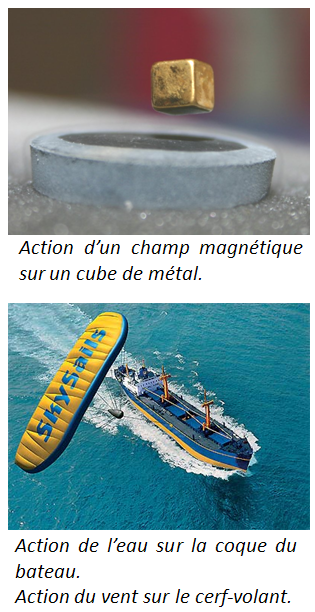
\includegraphics[width=1.52986in,height=2.97083in]{11-Actions Mécaniques/Cours/pandoc/media/image22.png}Actions mécaniques}{Actions mécaniques}}\label{actions-muxe9caniques}}

\hypertarget{duxe9finition}{%
\subsubsection{Définition}\label{duxe9finition}}

On apelle Action Mécanique (AM), toute cause capable de~:

\begin{itemize}
\item
  \textbf{provoquer} ou \textbf{modifier le mouvement} d'un solide~;
\item
  \textbf{provoquer la déformation} d'un solide~;
\item
  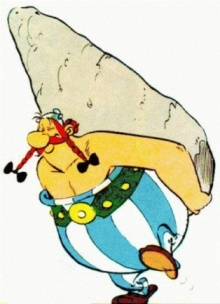
\includegraphics[width=1.00069in,height=1.38264in]{11-Actions Mécaniques/Cours/pandoc/media/image23.jpeg}\textbf{et éventuellement maintenir à l'équilibre}
\end{itemize}

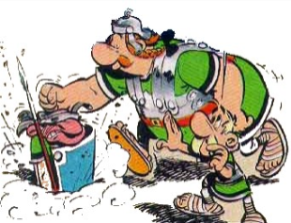
\includegraphics[width=1.32222in,height=1.01528in]{11-Actions Mécaniques/Cours/pandoc/media/image24.png}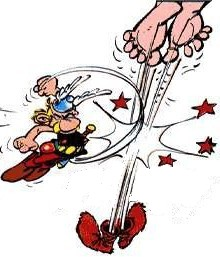
\includegraphics[width=1.03333in,height=1.28125in]{11-Actions Mécaniques/Cours/pandoc/media/image25.png}

On distingue~:

\begin{itemize}
\tightlist
\item
  les \textbf{actions mécaniques à distance}. Elles agissent sur tout le volume du solide. \ul{Exemple~:} actions magnétiques, action de la pesanteur\ldots{}
\end{itemize}

\begin{itemize}
\tightlist
\item
  les \textbf{actions mécaniques de contact}. Elles agissent directement sur la surface du solide.
\end{itemize}

\ul{Exemples~:} pression d'un fluide, action de contact entre deux solides\ldots{}

Qu'elle soit à distance ou de contact, une AM a toujours une origine et une cible. On utilisera donc la notation~: 
\includegraphics{11-Actions Mécaniques/Cours/pandoc/media/image26.wmf}

\textbf{\ul{Exemple~:}}

\begin{itemize}
\item
  action de la pesanteur sur le solide 3~: \(p \rightarrow 3\)
\item
  action du solide 4 sur le solide 2~: \(4 \rightarrow 2\)
\item
  action d'un moteur sur le solide 1~: \(m \rightarrow 1\)
\end{itemize}

\hypertarget{torseurs-dam-particuliers-torseur-glisseur-torseur-couple}{%
\subsubsection{Torseurs d'AM particuliers~: Torseur glisseur, Torseur couple}\label{torseurs-dam-particuliers-torseur-glisseur-torseur-couple}}

\begin{longtable}[]{@{}
  >{\raggedright\arraybackslash}p{(\columnwidth - 2\tabcolsep) * \real{0.4861}}
  >{\raggedright\arraybackslash}p{(\columnwidth - 2\tabcolsep) * \real{0.5000}}@{}}
\toprule\noalign{}
\begin{minipage}[b]{\linewidth}\raggedright
\textbf{\ul{Torseurs d'AM particuliers~:}}
\end{minipage} & \begin{minipage}[b]{\linewidth}\raggedright
\end{minipage} \\
\midrule\noalign{}
\endhead
\bottomrule\noalign{}
\endlastfoot
Un torseur dont le \textbf{\emph{moment est nul}} est appelé \textbf{\emph{\ul{torseur glisseur}}}~:

\(\boxed{\left\{ T_{1 \rightarr
ow 2} \right\} = \begin{Bmatrix}
\overri
ghtarrow{R_{1 \rightarrow 2}} \\
\overrightarrow{0}
\end{Bmatrix}_{J}}\)

Cela signifie que l'action mécanique de \(1 \rightarrow 2\) ne va pas provoquer, modifier ou empêcher un mouvement de rotation du solide 2 autour du point J.

Exemples de torseur glisseur~:

Pesanteur, effort d'un vérin, ressort de traction,\ldots{} & Un torseur dont la \textbf{\emph{résultante est nulle}} est appelé \textbf{\emph{\ul{torseur couple}}} :

\(\boxed{\left\{ T_{1 \rightar
row 2} \right\} = \begin{Bmatrix}
\overrightarrow{0} \\
\over
rightarrow{M_{J,1 \rightarrow 2}}
\end{Bmatrix}_{J}}\)

Ce torseur reste le même pour tous les points de l'espace (invariant). En effet~:

\(\ov
errightarrow{M_{I,1 \rightarrow 2
}} = \overrightarrow{M_{J,1 \righ
tarrow 2}} + \overrightarrow{IJ}
\land \underset{= \overrightarrow
{0}}{\overset{\overrightarrow{R_{
1 \rightarrow 2}}}{︸}} = \overri
ghtarrow{M_{j,1 \rightarrow 2}}\)

Exemples de torseur couple~:

Couple moteur, ressort de torsion, couple de frottement \\
\end{longtable}

\hypertarget{thuxe9oruxe8me-des-actions-ruxe9ciproques}{%
\subsubsection{Théorème des actions réciproques}\label{thuxe9oruxe8me-des-actions-ruxe9ciproques}}

Le solide isolé (ou ensemble de solides) est toujours le solide (ou ensemble de solides) à droite. Lorsqu'on passe d'un solide (ou ensemble de solides) à un autre, le théorème des actions réciproques est utilisé~:

\textbf{Théorème des actions réciproques~:} \(\boxed{\left\{ T_{1 \rightarrow 2} \right\} = - \left\{ T_{2 \rightarrow 1} \right\}}\)

Il est donc à connaître\ldots{}

\hypertarget{cas-de-laction-muxe9canique-de-la-pesanteur}{%
\subsubsection{Cas de l'action mécanique de la pesanteur}\label{cas-de-laction-muxe9canique-de-la-pesanteur}}

Bien qu'elle puisse être parfois être négligée, l'action mécanique de la pesanteur est présente dans toutes les études du comportement des systèmes.

Nous nous limiterons cependant aux cas des solides homogènes, c\textquotesingle est-à-dire aux solides pour lesquels~la masse volumique est constante :


\includegraphics{11-Actions Mécaniques/Cours/pandoc/media/image27.wmf} solide, 
\includegraphics{11-Actions Mécaniques/Cours/pandoc/media/image28.wmf}

\begin{longtable}[]{@{}
  >{\raggedright\arraybackslash}p{(\columnwidth - 4\tabcolsep) * \real{0.2778}}
  >{\raggedright\arraybackslash}p{(\columnwidth - 4\tabcolsep) * \real{0.1481}}
  >{\raggedright\arraybackslash}p{(\columnwidth - 4\tabcolsep) * \real{0.5556}}@{}}
\toprule\noalign{}
\begin{minipage}[b]{\linewidth}\raggedright
\emph{\ul{Quelques ordres de grandeur~:}}
\end{minipage} & \begin{minipage}[b]{\linewidth}\raggedright
\textbf{Acier}
\end{minipage} & \begin{minipage}[b]{\linewidth}\raggedright

\includegraphics{11-Actions Mécaniques/Cours/pandoc/media/image29.wmf}
\end{minipage} \\
\midrule\noalign{}
\endhead
\bottomrule\noalign{}
\endlastfoot
& \textbf{Aluminium} & 
\includegraphics{11-Actions Mécaniques/Cours/pandoc/media/image30.wmf} \\
& \textbf{PVC} & 
\includegraphics{11-Actions Mécaniques/Cours/pandoc/media/image31.wmf} \\
\end{longtable}

\begin{itemize}
\tightlist
\item
  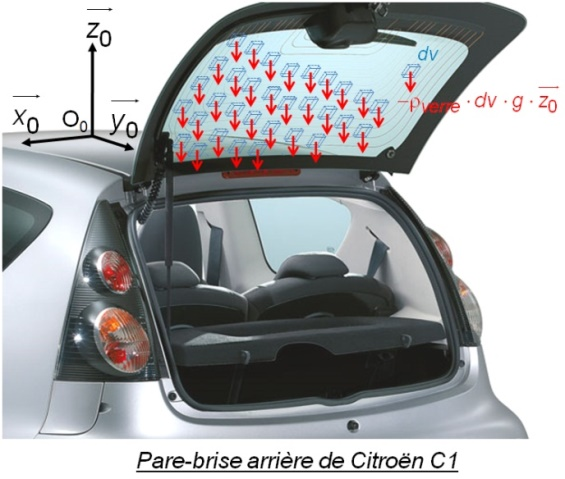
\includegraphics[width=2.56458in,height=2.18056in]{11-Actions Mécaniques/Cours/pandoc/media/image32.jpeg}\textbf{\ul{Point de vue local}}
\end{itemize}

L'action de la pesanteur sur un solide 1 est une action mécanique à distance. Le champ de force associé est tel que~:


\includegraphics{11-Actions Mécaniques/Cours/pandoc/media/image33.wmf} \(d\overrightarrow{F_{pes \rightarrow 1}(P)} = dm \cdot \overrightarrow{g} = \rho \cdot dv \cdot \overrightarrow{g}\)


\includegraphics{11-Actions Mécaniques/Cours/pandoc/media/image34.wmf}est appelé champ de pesanteur~:

\begin{itemize}
\item
  Il est orienté suivant la verticale ascendante~;
\item
  sa norme est \(\boxed{\left\| \overrightarrow{g} \right\| = g = 9,81m \cdot s^{- 2}}\).
\end{itemize}

\begin{itemize}
\tightlist
\item
  \textbf{\ul{Point de vue global}}
\end{itemize}

La \textbf{\emph{résultante}} de l'action de la pesanteur sur 1 est telle que~:

\(\overrightarrow{R_{pes \rightarrow 1}} = \int_{V_{1}}^{}{d\overrightarrow{F_{pes \rightarrow 1}(P)}} = \int_{V_{1}}^{}{\rho \cdot dv \cdot \overrightarrow{g}} = \rho \cdot \overrightarrow{g} \cdot \int_{V_{1}}^{}{dv} = \rho \cdot \overrightarrow{g} \cdot V_{1} = \boxed{m_{1} \cdot \overrightarrow{g}}\) 
\includegraphics{11-Actions Mécaniques/Cours/pandoc/media/image35.wmf}

Le \textbf{\emph{moment résultant}}, au point J, de l'action de la pesanteur sur 1 est tel que~:

\[\overrightarrow{M_{J,pes \rightarrow 1}} = \int_{V_{1}}^{}\left( \overrightarrow{JP} \land \rho \cdot \overrightarrow{g} \right) \cdot dv = \int_{V_{1}}^{}{\overrightarrow{JP} \cdot dv \land \rho \cdot \overrightarrow{g}}\]

Il existe un point \(G_{1}\), appelé \textbf{\emph{centre de gravité}} du solide 1, tel que~: \(\int_{V_{1}}^{}{\overrightarrow{G_{1}P} \cdot dv} = \overrightarrow{0}\)

Ainsi~: \(\overrightarrow{M_{G_{1},pes \rightarrow 1}} = \int_{V_{1}}^{}{\overrightarrow{G_{1}P} \cdot dv \land \rho \cdot \overrightarrow{g}} = \overrightarrow{0}\)

La position de ce centre de gravité (barycentre des masses élémentaires) peut être trouvée grâce à~:

\(\overrightarrow{OG_{1}} = \frac{1}{V_{1}}\int_{V_{1}}^{}{\overrightarrow{OP} \cdot dv}\) ou \(\overrightarrow{OG_{1}} = \frac{1}{m_{1}}\int_{V_{1}}^{}{\overrightarrow{OP} \cdot dm}\) (\(m_{1} = \rho \cdot V_{1}etdm = \rho \cdot dv\))

En effet~:\(\overrightarrow{0} = \int_{V_{1}}^{}{\overrightarrow{G_{1}P} \cdot dv} = \int_{V_{1}}^{}{\left( \overrightarrow{G_{1}O} + \overrightarrow{OP} \right) \cdot dv} = \int_{V_{1}}^{}{\overrightarrow{G_{1}O} \cdot dv} + \int_{V_{1}}^{}{\overrightarrow{OP} \cdot dv} = \overrightarrow{G_{1}O} \cdot V_{1} + \int_{V_{1}}^{}{\overrightarrow{OP} \cdot dv}\)

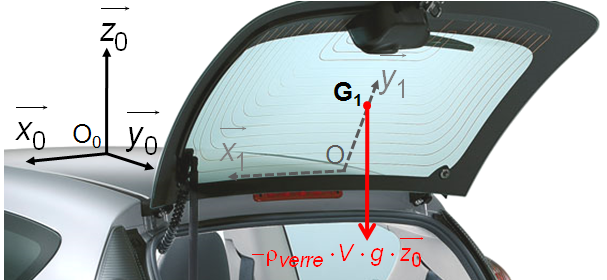
\includegraphics[width=3.36042in,height=1.54653in]{11-Actions Mécaniques/Cours/pandoc/media/image36.png}\(\Rightarrow \overrightarrow{OG_{1}} \cdot V_{1} = \int_{V_{1}}^{}{\overrightarrow{OP} \cdot dv}\)

\textbf{Le centre de gravité est toujours situé sur les éléments de symétrie du solide~: point, plan, droite\ldots{}}

\emph{Dans le cas du pare-brise~:} \(G_{1}\) \emph{est dans le plan} \((O,\overrightarrow{y_{1}},\overrightarrow{z_{1}})\)\emph{.}Le \textbf{\emph{\ul{torseur}}}, au point \(G_{1}\), de l'action de la pesanteur sur 1 est un glisseur tel que~:


\includegraphics{11-Actions Mécaniques/Cours/pandoc/media/image37.wmf}


\includegraphics[width=0.375in,height=0.31771in]{11-Actions Mécaniques/Cours/pandoc/media/image38.png}\textbf{Il faut retenir que la pesanteur est un torseur glisseur, qui est toujours exprimé dans le repère galiléen (associé au bâti en général en ATS).}

\hypertarget{actions-muxe9caniques-particuliuxe8res-uxe0-connauxeetre}{%
\subsubsection{Actions mécaniques particulières à connaître}\label{actions-muxe9caniques-particuliuxe8res-uxe0-connauxeetre}}

Il y a des actions mécaniques qu'il faut absolument connaître car elles sont très utilisées

\hypertarget{action-muxe9canique-de-la-pesanteur}{%
\subparagraph*{Action mécanique de la pesanteur}\label{action-muxe9canique-de-la-pesanteur}}
\addcontentsline{toc}{subparagraph}{Action mécanique de la pesanteur}

L'action mécanique de la pesanteur, comme vu précédemment, peut être modélisée par un torseur glisseur, exprimé au centre de gravité du solide (ou d'un ensemble de solides). Il est \textbf{toujours exprimé dans le repère galiléen} (associé au bâti en général en ATS).


\includegraphics{11-Actions Mécaniques/Cours/pandoc/media/image39.wmf}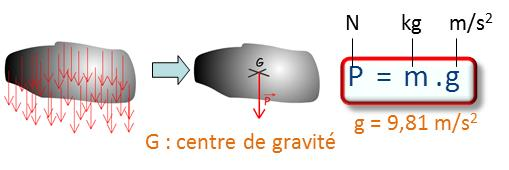
\includegraphics[width=3.28107in,height=1.09584in]{11-Actions Mécaniques/Cours/pandoc/media/image40.jpeg}

\hypertarget{action-muxe9canique-de-leffort-de-pression}{%
\subparagraph*{Action mécanique de l'effort de pression}\label{action-muxe9canique-de-leffort-de-pression}}
\addcontentsline{toc}{subparagraph}{Action mécanique de l'effort de pression}

L'effort de pression, en général pour les vérins, est fonction de la pression et de la surface du piston (éventuellement de la tige).


\includegraphics{11-Actions Mécaniques/Cours/pandoc/media/image41.wmf}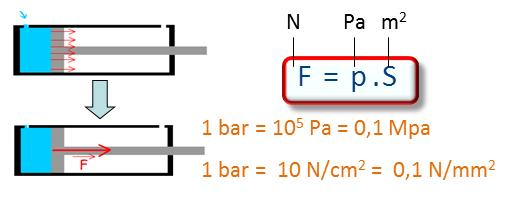
\includegraphics[width=2.95232in,height=1.14395in]{11-Actions Mécaniques/Cours/pandoc/media/image42.jpeg}

\begin{longtable}[]{@{}
  >{\raggedright\arraybackslash}p{(\columnwidth - 2\tabcolsep) * \real{0.1111}}
  >{\raggedright\arraybackslash}p{(\columnwidth - 2\tabcolsep) * \real{0.8750}}@{}}
\toprule\noalign{}
\begin{minipage}[b]{\linewidth}\raggedright
\begin{quote}
\includegraphics{1 1-Act ions Mécan iques /Cour s/pan doc/m edia/ image 8.png}\{wid th=``0 .6262 69685 03937 01in''

heigh t=``0. 65083 33333 33333 4in''\}
\end{quote}
\end{minipage} & \begin{minipage}[b]{\linewidth}\raggedright
\textbf{Vérin}

Un vérin permettant d'actionner une pince est commandé en alimentant la chambre arrière (diamètre du piston \(D_{p} = 50\mspace{6mu} mm\) et diamètre de sa tige \(D_{t} = 18\mspace{6mu} mm\)) avec la pression p\textsubscript{H} .

Dans cette position, la chambre avant du vérin est toujours alimentée avec une pression \(p_{0} = 6\mspace{6mu} bar\) (1 bar =10\textsuperscript{5}Pa). L'axe du vérin est noté y\textsubscript{3}. L'effort exercé par le vérin est égal à 220N.

\textbf{Déterminer, le modèle de l'action mécanique de la pression} \(\mathbf{p}_{\mathbf{H}}\) \textbf{sur la tige du vérin en fonction de la surface du piston}\(\mathbf{S}_{\mathbf{p}}\)\textbf{, de la surface occupée par la tige} \(\mathbf{S}_{\mathbf{t}}\)\textbf{, de} \(\mathbf{p}_{\mathbf{H}}\) \textbf{et de} \(\mathbf{p}_{\mathbf{0}}\) \textbf{. (Faire un dessin)}

\begin{quote}
\(\
left\{ T_{p_{H} \rightarrow tige} \right\} = \begin{Bmatrix} \left( p_{H} \cdot S_{p} - p_{0} \
cdot (S_{p} - S_{t}) \right) \cdot \overrightarrow{y_{3}} \\ \overrightarrow{0} \end{Bmatrix}\)
\end{quote}

\textbf{En déduire la valeur de} \(\mathbf{p}_{\mathbf{H}}\) \textbf{exprimée en bar.}

On a \(S_{p} = \pi \cdot \frac{{D_{p}}^{2}}{4}\)~: surface du piston et \(S_{t} = \pi \cdot \frac{{D_{t}}^{2}}{4}\)~: surface de la tige

Donc~:

\[p_{H} = \frac{6 \cdot 10^{5}
\cdot \frac{\pi}{4} \cdot \left( (50 \cdot 10^{- 3})^{2} - (
18 \cdot 10^{- 3})^{2} \right) + 220}{\pi \cdot \frac{(50 \c
dot 10^{- 3})^{2}}{4}} \Rightarrow \boxed{p_{H} = ... bar}\]
\end{minipage} \\
\midrule\noalign{}
\endhead
\bottomrule\noalign{}
\endlastfoot
& \\
\end{longtable}

\hypertarget{action-muxe9canique-pour-un-ressort-de-traction}{%
\subparagraph*{Action mécanique pour un ressort de traction}\label{action-muxe9canique-pour-un-ressort-de-traction}}
\addcontentsline{toc}{subparagraph}{Action mécanique pour un ressort de traction}

L'action mécanique modélisation un ressort de traction est un torseur glisseur dont la direction de l'effort est celle du ressort.


\includegraphics{11-Actions Mécaniques/Cours/pandoc/media/image43.wmf}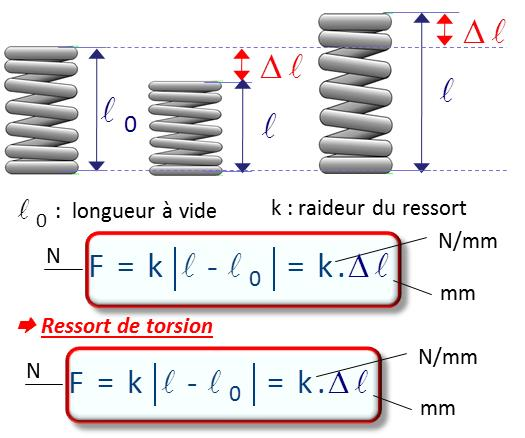
\includegraphics[width=2.77295in,height=1.64179in]{11-Actions Mécaniques/Cours/pandoc/media/image44.jpeg}

\hypertarget{action-muxe9canique-pour-un-couple-moteur}{%
\subparagraph*{Action mécanique pour un couple moteur}\label{action-muxe9canique-pour-un-couple-moteur}}
\addcontentsline{toc}{subparagraph}{Action mécanique pour un couple moteur}

Outre les vérins vus précédemment, un des actionneurs les plus utilisé est une machine tournante (souvent utilisée en moteur). Dans ce cas-là, l'action mécanique est modélisée par un torseur couple, dont le moment suivant l'axe de la pivot correspond au couple utile, souvent confondu avec le couple électromagnétique, et noté C\textsubscript{m}.


\includegraphics{11-Actions Mécaniques/Cours/pandoc/media/image45.wmf}

\textbf{Remarque}~: Pour une charge, on peut aussi avoir un torseur couple pour le couple résistant (négatif par convention).

\hypertarget{action-muxe9canique-pour-un-ressort-de-de-torsion}{%
\subparagraph*{Action mécanique pour un ressort de de torsion}\label{action-muxe9canique-pour-un-ressort-de-de-torsion}}
\addcontentsline{toc}{subparagraph}{Action mécanique pour un ressort de de torsion}

Pour un ressort de torsion, nous avons le cas dual du ressort de traction. Au lieu d'avoir un effort fonction du déplacement, il y a un moment fonction de la variation angulaire. La raideur k est en N.m/rad.


\includegraphics{11-Actions Mécaniques/Cours/pandoc/media/image46.wmf}

\hypertarget{actions-muxe9caniques-transmissibles-par-les-liaisons-usuelles}{%
\subsubsection{Actions mécaniques transmissibles par les liaisons usuelles}\label{actions-muxe9caniques-transmissibles-par-les-liaisons-usuelles}}

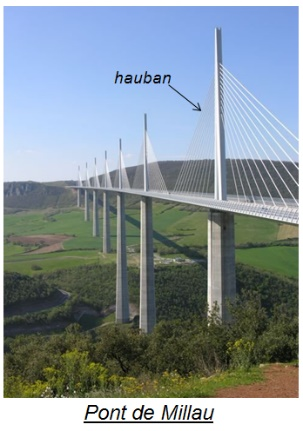
\includegraphics[width=1.375in,height=1.95833in]{11-Actions Mécaniques/Cours/pandoc/media/image47.jpeg}

Dans un système, les solides exercent des actions mécaniques sur les autres solides avec qui ils sont en contact. On dit alors qu'\textbf{\emph{ils transmettent des actions mécaniques par l'intermédiaire des liaisons.}}

\emph{\textbf{\ul{Exemple~:}} Sur le pont ci-contre, une partie du poids du pont est transmise aux haubans, qui eux même le transmettent au mât.}

\begin{itemize}
\tightlist
\item
  \textbf{\ul{Hypothèse de liaisons parfaites}}
\end{itemize}

Sauf si le contraire est précisé, on considère que le \textbf{\emph{contact}} entre les surfaces des solides en liaison se fait \textbf{\emph{sans adhérence ni frottement}}. En l'absence de frottement, \textbf{\emph{la puissance dissipée}} par échauffement au niveau de la liaison entre deux solides est \textbf{\emph{supposée nulle}}.

On admet l'expression de la puissance développée, au niveau de la liaison entre deux solides 1 et 2, par les actions mécaniques transmises par cette liaison~:

\(P(1 \leftrightarrow 2) = \left\{ T_{1 \rightarrow 2} \right\} \otimes \left\{ V_{2/1} \right\} = \begin{Bmatrix} \overrightarrow{R_{1 \rightarrow 2}} \\ \overrightarrow{M_{J,1 \rightarrow 2}} \end{Bmatrix}_{J} \otimes \begin{Bmatrix} \overrightarrow{\Omega_{2/1}} \\ \overrightarrow{V_{J \in 2/1}} \end{Bmatrix}_{J}\) (
\includegraphics{11-Actions Mécaniques/Cours/pandoc/media/image48.wmf}~: «~comoment~»)

Le comoment défini ci-dessus, qui se détaille à partir des éléments de réduction des deux torseurs, doit donc être nul~: \(P(1 \leftrightarrow 2) = \overrightarrow{R_{1 \rightarrow 2}} \cdot \overrightarrow{V_{J \in 2/1}} + \overrightarrow{M_{J,1 \rightarrow 2}} \cdot \overrightarrow{\Omega_{2/1}} = 0\)

Le détail de ces deux produits scalaires conduit à la somme de 6 termes indépendants de même signe qui doivent tous être nuls.

On en déduit ainsi, par \textbf{\emph{dualité avec la forme des torseurs cinématiques}}, la forme des \textbf{\emph{\ul{torseurs d'actions mécaniques transmissibles par les liaisons usuelles}}} supposées sans frottement~:

\begin{itemize}
\item
  pour \textbf{\emph{chaque degrés de liberté supprimé}}, il existe \textbf{\emph{une composante d'action mécanique}} susceptible d'être transmise par la liaison~;
\item
  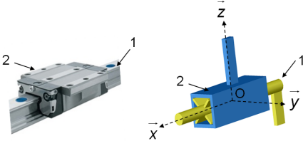
\includegraphics{11-Actions Mécaniques/Cours/pandoc/media/image49.png}\{width=``1.4in'' \textgreater{} height=``0.6430293088363954in''\}réciproquement, aucune composante \textgreater{} d'action mécanique ne peut être transmise là ou un mouvement \textgreater{} relatif est possible.
\end{itemize}

\ul{Exemple~:} Liaison glissière de direction \(\overrightarrow{x}\) entre 1 et 2.

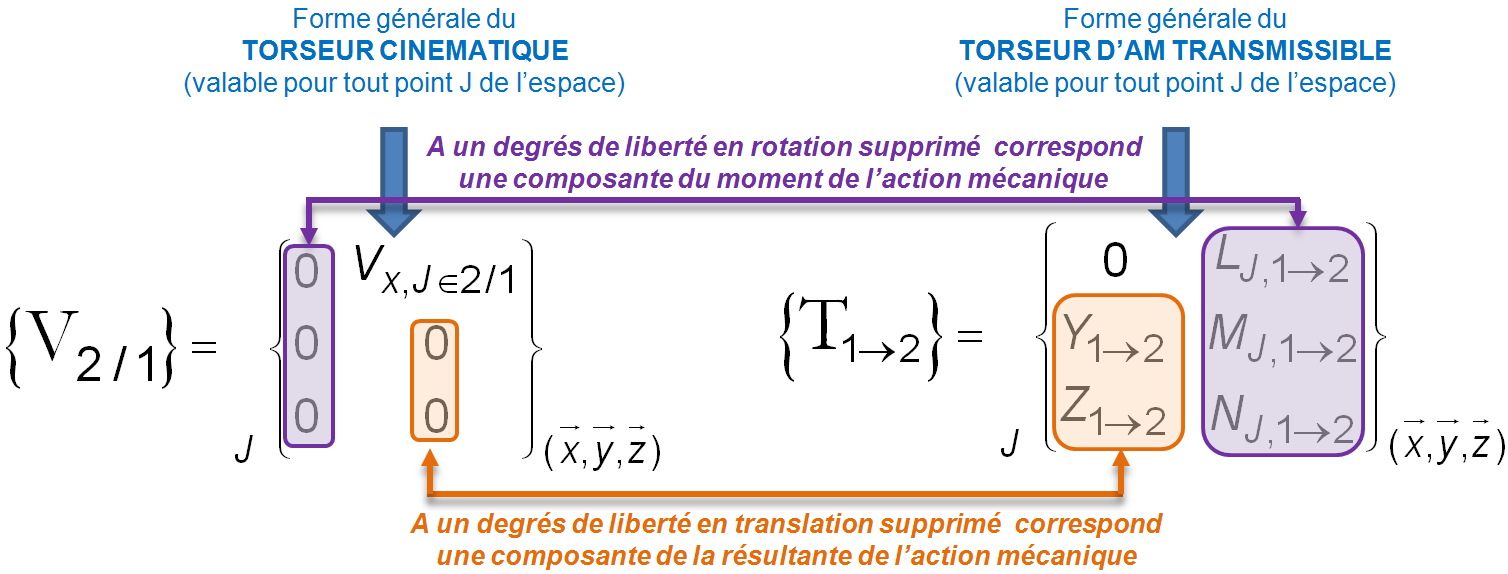
\includegraphics[width=6.52426in,height=2.46667in]{11-Actions Mécaniques/Cours/pandoc/media/image50.png}

\begin{longtable}[]{@{}
  >{\raggedright\arraybackslash}p{(\columnwidth - 6\tabcolsep) * \real{0.2327}}
  >{\raggedright\arraybackslash}p{(\columnwidth - 6\tabcolsep) * \real{0.3236}}
  >{\raggedright\arraybackslash}p{(\columnwidth - 6\tabcolsep) * \real{0.2182}}
  >{\raggedright\arraybackslash}p{(\columnwidth - 6\tabcolsep) * \real{0.2182}}@{}}
\toprule\noalign{}
\begin{minipage}[b]{\linewidth}\raggedright
\textbf{\emph{Nom et description géométrique}}
\end{minipage} & \begin{minipage}[b]{\linewidth}\raggedright
\end{minipage} & \begin{minipage}[b]{\linewidth}\raggedright
\textbf{\emph{Forme du torseur cinématique}}
\end{minipage} & \begin{minipage}[b]{\linewidth}\raggedright
\textbf{\emph{Forme du torseur d'action mécanique transmissible}}
\end{minipage} \\
\midrule\noalign{}
\endhead
\bottomrule\noalign{}
\endlastfoot
\textbf{GLISSIERE de direction} 
\includegraphics{11-Actions Mécaniques/Cours/pandoc/media/image54.wmf} & 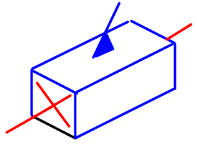
\includegraphics[width=0.89514in,height=0.65139in]{11-Actions Mécaniques/Cours/pandoc/media/image55.png} & 
\includegraphics{11-Actions Mécaniques/Cours/pandoc/media/image56.wmf} & 
\includegraphics{11-Actions Mécaniques/Cours/pandoc/media/image57.wmf} \\
& & \emph{Pour tout point A} & \\
\textbf{APPUI PLAN de normale} 
\includegraphics{11-Actions Mécaniques/Cours/pandoc/media/image58.wmf} & 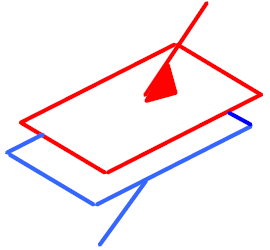
\includegraphics[width=0.90694in,height=0.8375in]{11-Actions Mécaniques/Cours/pandoc/media/image59.png} & 
\includegraphics{11-Actions Mécaniques/Cours/pandoc/media/image60.wmf} & 
\includegraphics{11-Actions Mécaniques/Cours/pandoc/media/image61.wmf} \\
& & \emph{Pour tout point A} & \\
\textbf{CYLINDRE-PLAN (ou LINEAIRE RECTILIGNE) de contact} 
\includegraphics{11-Actions Mécaniques/Cours/pandoc/media/image62.wmf}\textbf{et de normale} 
\includegraphics{11-Actions Mécaniques/Cours/pandoc/media/image58.wmf} & 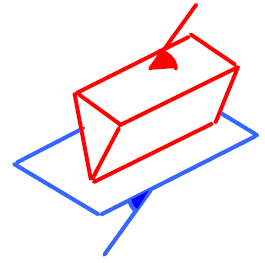
\includegraphics[width=0.88403in,height=0.87222in]{11-Actions Mécaniques/Cours/pandoc/media/image63.png} & 
\includegraphics{11-Actions Mécaniques/Cours/pandoc/media/image64.wmf} & 
\includegraphics{11-Actions Mécaniques/Cours/pandoc/media/image65.wmf} \\
& & \emph{Pour tout point A appartenant au plan} 
\includegraphics{11-Actions Mécaniques/Cours/pandoc/media/image66.wmf} & \\
\textbf{SPHERE-PLAN (ou PONCTUELLE) de contact O et de normale} 
\includegraphics{11-Actions Mécaniques/Cours/pandoc/media/image58.wmf} & 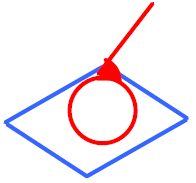
\includegraphics[width=0.84861in,height=0.79097in]{11-Actions Mécaniques/Cours/pandoc/media/image67.png} & 
\includegraphics{11-Actions Mécaniques/Cours/pandoc/media/image68.wmf} & 
\includegraphics{11-Actions Mécaniques/Cours/pandoc/media/image69.wmf} \\
& & \emph{Pout tout point appartenant à la normale} 
\includegraphics{11-Actions Mécaniques/Cours/pandoc/media/image70.wmf} & \\
\textbf{PIVOT GLISSANT d'axe} 
\includegraphics{11-Actions Mécaniques/Cours/pandoc/media/image62.wmf} & 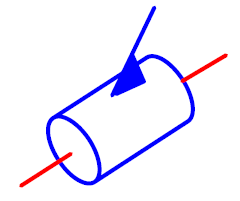
\includegraphics[width=0.95347in,height=0.80208in]{11-Actions Mécaniques/Cours/pandoc/media/image71.png} & 
\includegraphics{11-Actions Mécaniques/Cours/pandoc/media/image72.wmf} & 
\includegraphics{11-Actions Mécaniques/Cours/pandoc/media/image73.wmf} \\
& & \emph{Pour tout point A appartenant à l'axe} 
\includegraphics{11-Actions Mécaniques/Cours/pandoc/media/image74.wmf} & \\
\textbf{PIVOT d'axe} 
\includegraphics{11-Actions Mécaniques/Cours/pandoc/media/image62.wmf} & 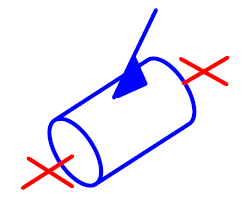
\includegraphics[width=0.97708in,height=0.81389in]{11-Actions Mécaniques/Cours/pandoc/media/image75.png} & 
\includegraphics{11-Actions Mécaniques/Cours/pandoc/media/image76.wmf} & 
\includegraphics{11-Actions Mécaniques/Cours/pandoc/media/image77.wmf} \\
& & \emph{Pour tout point A appartenant à l'axe} 
\includegraphics{11-Actions Mécaniques/Cours/pandoc/media/image78.wmf} & \\
\end{longtable}

Bien entendu, on peut aussi utiliser une écriture en ligne de ces torseurs~:

\begin{quote}
\[\boxed{\left\{ T_{1 \rightarrow 2} \right\} = \begin{Bmatrix}
\overrightarrow{R_{1 \rightarrow 2}} \\
\overrightarrow{M_{A,1 \rightarrow 2}}
\end{Bmatrix}_{A} = \begin{Bmatrix}
X_{1 \rightarrow 2} \cdot \overrightarrow{x} + Y_{1 \rightarrow 2} \cdot \overrightarrow{y} + Z_{1 \rightarrow 2} \cdot \overrightarrow{z} \\
L_{A,1 \rightarrow 2} \cdot \overrightarrow{x} + M_{A,1 \rightarrow 2} \cdot \overrightarrow{y} + N_{A,1 \rightarrow 2} \cdot \overrightarrow{z}
\end{Bmatrix}_{A}}\]
\end{quote}

\begin{longtable}[]{@{}
  >{\raggedright\arraybackslash}p{(\columnwidth - 6\tabcolsep) * \real{0.1944}}
  >{\raggedright\arraybackslash}p{(\columnwidth - 6\tabcolsep) * \real{0.1667}}
  >{\raggedright\arraybackslash}p{(\columnwidth - 6\tabcolsep) * \real{0.2778}}
  >{\raggedright\arraybackslash}p{(\columnwidth - 6\tabcolsep) * \real{0.3333}}@{}}
\toprule\noalign{}
\begin{minipage}[b]{\linewidth}\raggedright
\textbf{\emph{Nom et description géo métrique}}
\end{minipage} & \begin{minipage}[b]{\linewidth}\raggedright
\end{minipage} & \begin{minipage}[b]{\linewidth}\raggedright
\textbf{\emph{Forme du torseur cinématique}}
\end{minipage} & \begin{minipage}[b]{\linewidth}\raggedright
\textbf{\emph{Forme du torseur d'action mécanique transmissible}}
\end{minipage} \\
\midrule\noalign{}
\endhead
\bottomrule\noalign{}
\endlastfoot
\textbf{ HELICOIDALE d'axe} \includegraphics{11-Action s Mécanique s/Cours/pan doc/media/i mage62.wmf} & \includegraphics{1 1-Actions Mécaniqu es/Cours/ pandoc/me dia/image 79.png}\{w idth=``0.7 909722222 222222in'' hei ght=``0.62 777777777 77778in''\} & 
\includegraphics{11 -Actions Mécaniqu es/Cours/pandoc/m edia/image80.wmf} & 
\includegraphics{11-Actions Mécaniques/Cours/pand oc/media/image81.wmf} \\
& & \emph{Pour tout point A appartenant à l'axe} 
\includegraphics{11 -Actions Mécaniqu es/Cours/pandoc/m edia/image82.wmf}

\textbf{\emph{p~: pas de la liaison}} & \\
\textbf{SPHERIQUE (ou ROTULE) de centre O} & \includegraphics{1 1-Actions Mécaniqu es/Cours/ pandoc/me dia/image 83.png}\{w idth=``1.1 513888888 888888in'' hei ght=``0.62 777777777 77778in''\} & 
\includegraphics{11 -Actions Mécaniqu es/Cours/pandoc/m edia/image84.wmf} & 
\includegraphics{11-Actions Mécaniques/Cours/pand oc/media/image85.wmf} \\
& & \emph{Seulement au point O} & \\
\textbf{SPHERIQUE A DOIGT (ou ROTULE A DOIGT) de centre O et de rotation interdite} \includegraphics{11-Action s Mécanique s/Cours/pan doc/media/i mage86.wmf} & \includegraphics{1 1-Actions Mécaniqu es/Cours/ pandoc/me dia/image 87.png}\{w idth=``1.1 743055555 555555in'' hei ght=``0.65 138888888 88889in''\} & 
\includegraphics{11 -Actions Mécaniqu es/Cours/pandoc/m edia/image88.wmf} & 
\includegraphics{11-Actions Mécaniques/Cours/pand oc/media/image89.wmf} \\
& & \emph{Seulement au point O} & \\
\textbf{SPHE RE-CYLINDRE (ou LINEAIRE ANNULAIRE) de centre O et de direction} \includegraphics{11-Action s Mécanique s/Cours/pan doc/media/i mage54.wmf} & \includegraphics{1 1-Actions Mécaniqu es/Cours/ pandoc/me dia/image 90.png}\{w idth=``0.9 534722222 222223in'' hei ght=``0.79 097222222 22222in''\} & 
\includegraphics{11 -Actions Mécaniqu es/Cours/pandoc/m edia/image91.wmf} & 
\includegraphics{11-Actions Mécaniques/Cours/pand oc/media/image92.wmf} \\
& & \emph{Seulement au point O} & \\
\end{longtable}

\textbf{\emph{Cas particulier de la liaison hélicoïdale~:}}

Pour cette liaison, la dualité entre la forme du torseur cinématique et la forme du torseur d'action mécanique transmissible est moins évidente.

\emph{\ul{Rappel~:} cette liaison n'admet \textbf{qu'un seul degré de liberté}. La translation et la rotation n'étant pas indépendantes.}

On cherche la forme du torseur d'action mécanique transmissible qui assure une puissance développée au niveau de la liaison qui soit nulle~:

\[P(1 \leftrightarrow 2) = \overrightarrow{R_{1 \rightarrow 2}} \cdot \overrightarrow{V_{J \in 2/1}} + \overrightarrow{M_{J,1 \rightarrow 2}} \cdot \overrightarrow{\Omega_{2/1}} = 0\]

Ce qui nous conduit, entre autres, à~: \(\mspace{6mu} \pm X_{1 \rightarrow 2} \cdot \omega_{x,2/1} \cdot \frac{p}{2\pi} + L_{A,1 \rightarrow 2} \cdot \omega_{x,2/1} = 0\)

Donc~: \(\boxed{L_{A,1 \rightarrow 2} = \pm X_{1 \rightarrow 2} \cdot \frac{p}{2\pi}}\) le signe 
\includegraphics{11-Actions Mécaniques/Cours/pandoc/media/image93.wmf}dépend du type de liaison hélicoïdale (pas à droite ou pas à gauche)

\hypertarget{section}{%
\subsubsection*{}\label{section}}
\addcontentsline{toc}{subsubsection}{}

\begin{longtable}[]{@{}
  >{\raggedright\arraybackslash}p{(\columnwidth - 2\tabcolsep) * \real{0.1111}}
  >{\raggedright\arraybackslash}p{(\columnwidth - 2\tabcolsep) * \real{0.8750}}@{}}
\toprule\noalign{}
\begin{minipage}[b]{\linewidth}\raggedright
\begin{quote}
\includegraphics{1 1-Act ions Mécan iques /Cour s/pan doc/m edia/ image 8.png}\{wid th=``0 .6262 69685 03937 01in''

heigh t=``0. 65083 33333 33333 4in''\}
\end{quote}
\end{minipage} & \begin{minipage}[b]{\linewidth}\raggedright
\textbf{Entrainement torseur d'AM transmissible}

\textbf{Donner les torseurs d'AM transmissibles des liaisons suivantes}

\(L_{2/1}\ \): Liaison appui-plan de normale \((A,\overrightarrow{x_{0}})\)

\(\ L_{4/3}\ \): Liaison pivot d'axe \((B,\overrightarrow{y_{2}})\)

\(L_{2/0}\ \): Liaison glissière de direction \((C,\overrightarrow{z_{3}})\)

\(L_{5/3}\ \): Liaison cylindre-plan de normale \(\left( P,\overrightarrow{z_{4}} \right)\ \) et d'axe \(\overrightarrow{x_{4}}\)

\(L_{6/2}\ \): Liaison sphérique de centre \(D\)

\(L_{8/3}\ \): Liaison sphère-cylindre d'axe \(\left( Q,\overrightarrow{z_{2}} \right)\ \)

\(L_{8/3}\ \): Liaison hélicoïdale d'axe \(\left( M,\overrightarrow{z_{6}} \right)\ \)
\end{minipage} \\
\midrule\noalign{}
\endhead
\bottomrule\noalign{}
\endlastfoot
& \\
\end{longtable}

\hypertarget{cas-particulier-dun-probluxe8me-plan}{%
\subsubsection{Cas particulier d'un problème plan}\label{cas-particulier-dun-probluxe8me-plan}}

On peut admettre que l'on est face à un problème «~plan~» si~:

\begin{itemize}
\item
  la \textbf{géométrie des liaisons} du système \textbf{présente un} \textbf{plan de symétrie,}
\item
  les \textbf{AM extérieures} exercées sur ce système \textbf{sont symétriques par rapport à ce plan}, c'est à dire que~:
\end{itemize}

\begin{quote}
- les résultantes des AM extérieures sont parallèles au plan de symétrie,

- les moments des AM extérieures sont perpendiculaires au plan de symétrie.
\end{quote}

\begin{itemize}
\tightlist
\item
  Le système est représenté dans le plan
\end{itemize}

Dans le cas d'un \textbf{problème plan}, l'application de l'équilibre ne peut fournir au maximum que \textbf{3 équations scalaires}~:

\begin{itemize}
\item
  \textbf{\emph{2 équations issues du théorème de la résultante}} statique projeté sur les 2 axes de la base appartenant au plan~;
\item
  \textbf{\emph{1 équation issue du théorème du moment statique}} projeté sur le 3\textsuperscript{ème} axe de la base (perpendiculaire au plan).
\end{itemize}

\begin{longtable}[]{@{}
  >{\raggedright\arraybackslash}p{(\columnwidth - 8\tabcolsep) * \real{0.0519}}
  >{\raggedright\arraybackslash}p{(\columnwidth - 8\tabcolsep) * \real{0.2727}}
  >{\raggedright\arraybackslash}p{(\columnwidth - 8\tabcolsep) * \real{0.3117}}
  >{\raggedright\arraybackslash}p{(\columnwidth - 8\tabcolsep) * \real{0.2727}}
  >{\raggedright\arraybackslash}p{(\columnwidth - 8\tabcolsep) * \real{0.0519}}@{}}
\toprule\noalign{}
\begin{minipage}[b]{\linewidth}\raggedright
\begin{itemize}
\tightlist
\item
\item
  E x e m p l e
\item
\item
\end{itemize}
\end{minipage} & \begin{minipage}[b]{\linewidth}\raggedright
\end{minipage} & \begin{minipage}[b]{\linewidth}\raggedright
\end{minipage} & \begin{minipage}[b]{\linewidth}\raggedright
\end{minipage} & \begin{minipage}[b]{\linewidth}\raggedright
\end{minipage} \\
\midrule\noalign{}
\endhead
\bottomrule\noalign{}
\endlastfoot
! {[}{]} ( 1 1 - A c t i o n s

M é c a n i q u e s / C o u r s / p a n d o c / m e d i a / i m a g e 9 4 . p n g ) \{ w i d t h = '' 1 . 7 5 6 9 4 4 4 4 4 4 4 4 4 4 4 4 i n '' h e i g h t = '' 1 . 7 9 6 5 2 7 7 7 7 7 7 7 7 7 7 7 i n '' \} P o u r c e p r o b l è m e p l a n ! {[}{]} ( 1 1 - A c t i o n s

M é c a n i q u e s / C o u r s / p a n d o c / m e d i a / i m a g e 9 5 . w m f ) , t o u s l e s t o r s e u r s d ' A M o n t l a f o r m e

:

! {[}{]} ( 1 1 - A c t i o n s

M é c a n i q u e s / C o u r s / p a n d o c / m e d i a / i m a g e 9 6 . w m f ) & & & & \\
\begin{minipage}[t]{\linewidth}\raggedright
E n g é n é r a l , i l e s t m e n t i o n n é d a n s l ' é n o n c é d ' u n e x e r c i c e q u e l ' o n e s t f a c e à u n p r o b l è m e p l a n . M a i s i l f a u t ê t r e c a p a b l e d e s i m p l i f i e r l e s t o r s e u r s d ' A M e n a n n u l a n t c e r t a i n e s c o m p o s a n t e s d e s é l é m e n t s d e r é d u c t i o n .

\begin{itemize}
\tightlist
\item
\item
\item
  L e s c o m p o s a n t e s à a n n u l e r s o n t c e l l e s q u i c o r r e s p o n d e n t à d e s a c t i o n s m é c a n i q u e s s u s c e p t i b l e s d e f a i r e s o r t i r l e s s o l i d e s d u p l a n
\item
\item
\item
\end{itemize}
\end{minipage} & & & & \\
& \textbf{Problème plan} {[}{]} (11-Actions Mécani ques/Cours/pandoc/ media/image97.wmf) & \textbf{Problème plan} 
\includegraphics{11-Actions Mécaniques/Cours/pand oc/media/image98.wmf} & \textbf{Problème plan} {[}{]} (11-Actions Mécani ques/Cours/pandoc/ media/image99.wmf) & \\
! {[}{]} ( 1 1 - A c t i o n s

M é c a n i q u e s / C o u r s / p a n d o c / m e d i a / i m a g e 1 0 0 . w m f )

! {[}{]} ( 1 1 - A c t i o n s

M é c a n i q u e s / C o u r s / p a n d o c / m e d i a / i m a g e 1 0 1 . w m f ) & & 
\includegraphics{11-Actions M écaniques/Cours/pando c/media/image102.wmf}


\includegraphics{11-Actions M écaniques/Cours/pando c/media/image103.wmf} & 
\includegraphics{11-Actions Mécaniq ues/Cours/pandoc/m edia/image104.wmf}


\includegraphics{11-Actions Mécaniq ues/Cours/pandoc/m edia/image105.wmf} & \\
& & & & \\
\end{longtable}

\hypertarget{etude-de-luxe9quilibre-dun-systuxe8me}{%
\subsection{Etude de l'équilibre d'un système~}\label{etude-de-luxe9quilibre-dun-systuxe8me}}

\hypertarget{etude-de-luxe9quilibre-principe-de-la-statique}{%
\subsubsection{Etude de l'équilibre~: Principe de la Statique}\label{etude-de-luxe9quilibre-principe-de-la-statique}}

La condition nécessaire pour qu'un \textbf{\emph{ensemble isolé}} 
\includegraphics{11-Actions Mécaniques/Cours/pandoc/media/image106.wmf} \textbf{\emph{soit en équilibre}} par rapport à un repère galiléen est que \textbf{\emph{la somme des torseurs des actions mécaniques extérieures à}} 
\includegraphics{11-Actions Mécaniques/Cours/pandoc/media/image106.wmf} \textbf{\emph{soit nulle}}~:


\includegraphics{11-Actions Mécaniques/Cours/pandoc/media/image107.wmf} pour tout point A

Cette équation torsorielle conduit à 2 équations vectorielles~:

\begin{itemize}
\item
  \textbf{\ul{Théorème de la résultante statique (TRS)~:}} \textgreater{} 
\includegraphics{11-Actions Mécaniques/Cours/pandoc/media/image108.wmf}
\item
  \textbf{\ul{Théorème du moment statique (TMS)~:}} \textgreater{} 
\includegraphics{11-Actions Mécaniques/Cours/pandoc/media/image109.wmf}
\end{itemize}

Après avoir exprimé les différents vecteurs dans la même base 
\includegraphics{11-Actions Mécaniques/Cours/pandoc/media/image110.wmf}, chacune de ces équations vectorielles conduit à 3 \textbf{\emph{équations scalaires}}, soit \textbf{\emph{6 au total}}~:


\includegraphics{11-Actions Mécaniques/Cours/pandoc/media/image111.wmf}

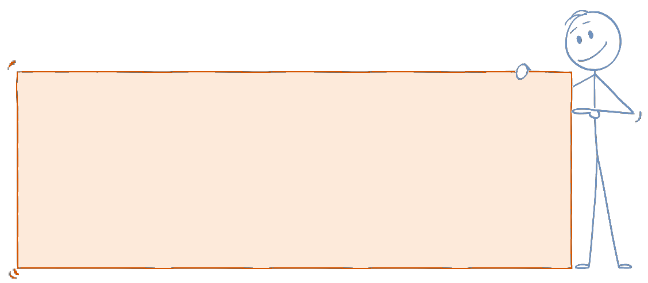
\includegraphics[width=4.1875in,height=1.89097in]{11-Actions Mécaniques/Cours/pandoc/media/image10.png}

\hypertarget{duxe9marche-de-ruxe9solution-dun-probluxe8me-pour-uxe9tudier-luxe9quilibre}{%
\subsubsection{Démarche de résolution d'un problème pour étudier l'équilibre}\label{duxe9marche-de-ruxe9solution-dun-probluxe8me-pour-uxe9tudier-luxe9quilibre}}

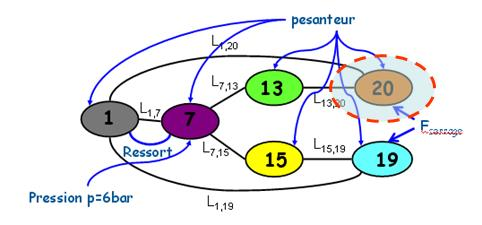
\includegraphics[width=4.01667in,height=1.875in]{11-Actions Mécaniques/Cours/pandoc/media/image112.jpeg}Dans tous les cas, pour étudier l'équilibre d'un système, un graphe de structure est réalisé.

Une démarche possible pour résoudre la problématique posée est~:

\begin{enumerate}
\def\labelenumi{\arabic{enumi}.}
\item
  Modéliser le système et établir le graphe des liaisons puis le \textgreater{} graphe de structure;
\item
  Déterminer un isolement coupant la liaison aux inconnues recherchées \textgreater{} et \textbf{coupant le moins de liaisons non recherchées (nombre \textgreater{} d'inconnues statiques coupées inférieur ou égal au nombre \textgreater{} d'équations)};
\item
  Faire le Bilan des AM extérieures (BAME);
\item
  Identifier les AM données et les AM recherchées ;
\item
  Regarder si une relation peut être trouvée avec le Théorème de la \textgreater{} Résultante Statique. Si oui, il faut projeter (avec un produit \textgreater{} scalaire) les différentes résultantes et résoudre les équations \textgreater{} scalaires. Si non, il faut déplacer les torseurs.
\item
  Choisir le point de réduction et les équations ne sollicitant pas \textgreater{} les inconnues non recherchées ;
\item
  Ecrire le système d'équations en appliquant le TRS et/ou le TMS. \textgreater{} S'il ne peut être résolu, identifier les inconnues à rechercher et \textgreater{} proposer un nouvel isolement intelligent (coupant des inconnues \textgreater{} déjà trouvées).
\end{enumerate}

\hypertarget{conseils-pour-le-choix-du-point-de-ruxe9duction}{%
\subsubsection{Conseils pour le choix du point de réduction}\label{conseils-pour-le-choix-du-point-de-ruxe9duction}}

Choisir le point de réduction et les équations ne sollicitant pas les inconnues non recherchées~:

\begin{itemize}
\item
  éviter de déplacer un torseur contenant beaucoup d'inconnues d'effort,
\item
  projeter sur des directions particulières.
\end{itemize}

\hypertarget{inventaire-ou-bilan-des-actions-muxe9caniques-extuxe9rieurs-bame}{%
\subsubsection{Inventaire (ou bilan) des actions mécaniques extérieurs (BAME)}\label{inventaire-ou-bilan-des-actions-muxe9caniques-extuxe9rieurs-bame}}

On définit~:

\begin{itemize}
\item
  des \textbf{actions mécaniques extérieures} qui correspondent à toutes \textgreater{} les actions mécaniques exercées par le milieu extérieur \textgreater{} 
\includegraphics{11-Actions Mécaniques/Cours/pandoc/media/image113.wmf} \textgreater{} (solide, fluide, ressort, pesanteur, \ldots) et qui agissent \textbf{SUR} \textgreater{} un des éléments du milieu \textgreater{} intérieur
\includegraphics{11-Actions Mécaniques/Cours/pandoc/media/image20.wmf}.
\item
  des \textbf{actions mécaniques intérieures} qui correspondent à toutes \textgreater{} les actions mécaniques exercées par un élément (solide, fluide, \textgreater{} ressort, \ldots) appartenant au milieu intérieur \textgreater{} 
\includegraphics{11-Actions Mécaniques/Cours/pandoc/media/image20.wmf} et qui \textgreater{} agit sur un autre élément du milieu \textgreater{} intérieur
\includegraphics{11-Actions Mécaniques/Cours/pandoc/media/image20.wmf}.
\end{itemize}

\begin{longtable}[]{@{}
  >{\raggedright\arraybackslash}p{(\columnwidth - 2\tabcolsep) * \real{0.1111}}
  >{\raggedright\arraybackslash}p{(\columnwidth - 2\tabcolsep) * \real{0.8750}}@{}}
\toprule\noalign{}
\begin{minipage}[b]{\linewidth}\raggedright
\begin{quote}
\includegraphics{1 1-Act ions Mécan iques /Cour s/pan doc/m edia/ image 8.png}\{wid th=``0 .6262 69685 03937 01in''

heigh t=``0. 65083 33333 33333 4in''\}
\end{quote}
\end{minipage} & \begin{minipage}[b]{\linewidth}\raggedright
\textbf{Console de bateau}

\textbf{\emph{\ul{Exemple~:}}} On choisit d'isoler un ensemble 
\includegraphics{11-Actions Mécaniques/Cours/pandoc/media/image114.wmf}


\includegraphics[width=5.89514in,height=1.84861in]{11-Actions Mécanique s/Cours/pandoc/media/image9.png}

Bilan des actions mécaniques extérieures à 
\includegraphics{11-Actions Mécaniques/Cours/pandoc/media/image114.wmf}~:

\begin{itemize}
\item
  AM de 
\includegraphics{11-Actions Mécaniques/Cours/pandoc/media/image115.wmf}(par l'intermédiaire d'une liaison sphérique de centre C)~;
\item
  AM de 
\includegraphics{11-Actions Mécaniques/Cours/pandoc/media/image116.wmf}(par l'intermédiaire d'une liaison sphérique de centre B)~;
\item
  AM de
\end{itemize}


\includegraphics{11-Actions Mécaniques/Cours/pandoc/media/image117.wmf} (négligée)~;

\begin{itemize}
\tightlist
\item
  AM de
\end{itemize}


\includegraphics{11-Actions Mécaniques/Cours/pandoc/media/image118.wmf} (négligée)~;

Sous forme de torseur~:


\includegraphics{11-Actions Mécaniques/Cours/pandoc/media/image119.wmf} 
\includegraphics{11-Actions Mécaniques/Cours/pandoc/media/image120.wmf}

Donc~: 
\includegraphics{11-Actions Mécaniques/Cours/pandoc/media/image121.wmf}

\emph{\textbf{\ul{Exemple~}:} Pilote automatique de bateau}

Le théorème du moment statique nous donne~:


\includegraphics{11-Actions Mécaniques/Cours/pandoc/media/image122.wmf} Or 
\includegraphics{11-Actions Mécaniques/Cours/pandoc/media/image123.wmf}

et 
\includegraphics{11-Actions Mécaniques/Cours/pandoc/media/image124.wmf}

Donc 
\includegraphics{11-Actions Mécaniques/Cours/pandoc/media/image125.wmf}

Cette application du PFS ne nous permet pas de terminer parfaitement toutes les composantes inconnues du torseur d'AM de 
\includegraphics{11-Actions Mécaniques/Cours/pandoc/media/image116.wmf} mais les résultats obtenus seront utilisés plus tard pour répondre à une problématique concrète.
\end{minipage} \\
\midrule\noalign{}
\endhead
\bottomrule\noalign{}
\endlastfoot
& \\
\end{longtable}

\hypertarget{ensemble-isoluxe9-soumis-uniquement-uxe0-des-torseurs-glisseurs}{%
\subsubsection{Ensemble isolé soumis uniquement à des torseurs glisseurs}\label{ensemble-isoluxe9-soumis-uniquement-uxe0-des-torseurs-glisseurs}}

Dans un problème plan, le bilan des actions mécaniques peut dans certains cas nous conduire à recenser \textbf{\emph{au maximum 3 actions mécaniques extérieures}} modélisables par des \textbf{\emph{torseurs glisseurs}}.

\textbf{Il faut utiliser les résultats ci-dessous car ils permettent de résoudre rapidement certains problèmes. Il faut notamment repérer les solides soumis à deux glisseurs (vérins, bielles, ...).}

Dans ces conditions, on pourra utiliser les résultats suivants~:

\begin{longtable}[]{@{}
  >{\raggedright\arraybackslash}p{(\columnwidth - 0\tabcolsep) * \real{1.0000}}@{}}
\toprule\noalign{}
\begin{minipage}[b]{\linewidth}\raggedright
\textbf{ENSEMBLE ISOLE SOUMIS A 2 GLISSEURS}
\end{minipage} \\
\midrule\noalign{}
\endhead
\bottomrule\noalign{}
\endlastfoot
\begin{minipage}[t]{\linewidth}\raggedright
Si un ensemble isolé est en équilibre sous l'action de 2 glisseurs alors :

\begin{itemize}
\item
  \textbf{ces 2 glisseurs sont opposés (même norme, même direction, sens \textgreater{} contraire)}
\item
  \textbf{ces 2 glisseurs ont comme même direction~: la droite d'action \textgreater{} passant par les points ou sont exprimés les 2 torseurs \textgreater{} glisseurs}
\end{itemize}
\end{minipage} \\
\end{longtable}

\textbf{\ul{Exemple~:}} Coffre motorisé d'Audi A8

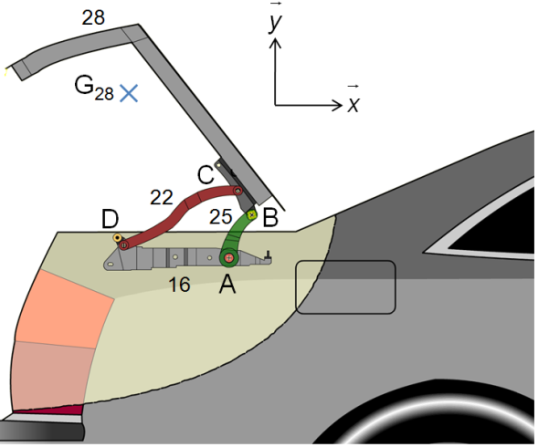
\includegraphics[width=2.44375in,height=2.03472in]{11-Actions Mécaniques/Cours/pandoc/media/image126.png}Problème plan 
\includegraphics{11-Actions Mécaniques/Cours/pandoc/media/image127.wmf}

\ul{Hypothèse~:} l'action de la pesanteur est négligeable sur toutes les pièces sauf sur le coffre 28.

On isole la bielle 22, BAME à 22~:

\begin{itemize}
\item
  action de 
\includegraphics{11-Actions Mécaniques/Cours/pandoc/media/image128.wmf}
\item
  action de 
\includegraphics{11-Actions Mécaniques/Cours/pandoc/media/image129.wmf}
\item
  action de 
\includegraphics{11-Actions Mécaniques/Cours/pandoc/media/image130.wmf}~: négligée
\end{itemize}

En tenant compte des simplifications liées au problème plan dans l'écriture des torseurs d'actions mécaniques transmissibles par les liaisons pivot en D et C~:


\includegraphics{11-Actions Mécaniques/Cours/pandoc/media/image131.wmf}et 
\includegraphics{11-Actions Mécaniques/Cours/pandoc/media/image132.wmf}

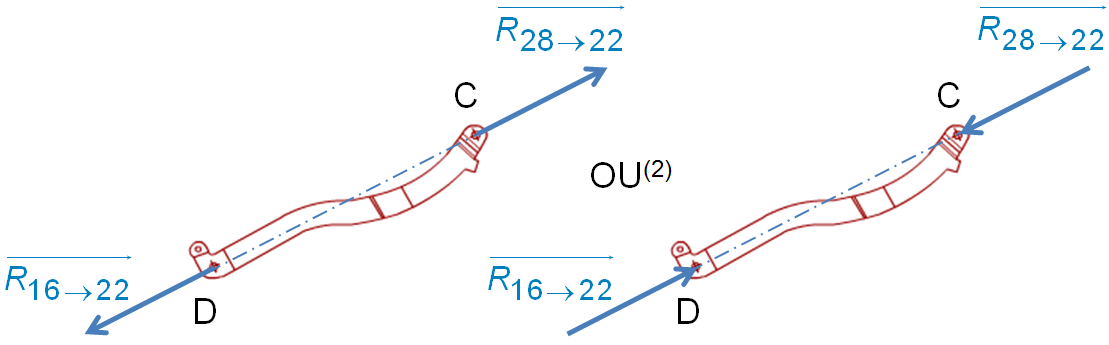
\includegraphics[width=3.83611in,height=1.19931in]{11-Actions Mécaniques/Cours/pandoc/media/image133.png}Ces deux torseurs sont des torseurs glisseurs, on a donc~:


\includegraphics{11-Actions Mécaniques/Cours/pandoc/media/image134.wmf}

et 
\includegraphics{11-Actions Mécaniques/Cours/pandoc/media/image135.wmf}

En effet, le théorème du moment statique nous donne~: 
\includegraphics{11-Actions Mécaniques/Cours/pandoc/media/image138.wmf}

Or 
\includegraphics{11-Actions Mécaniques/Cours/pandoc/media/image139.wmf}et 
\includegraphics{11-Actions Mécaniques/Cours/pandoc/media/image140.wmf}

\begin{longtable}[]{@{}
  >{\raggedright\arraybackslash}p{(\columnwidth - 0\tabcolsep) * \real{1.0000}}@{}}
\toprule\noalign{}
\begin{minipage}[b]{\linewidth}\raggedright
\textbf{ENSEMBLE ISOLE SOUMIS A 3 GLISSEURS}
\end{minipage} \\
\midrule\noalign{}
\endhead
\bottomrule\noalign{}
\endlastfoot
\begin{minipage}[t]{\linewidth}\raggedright
Si un ensemble isolé est en équilibre sous l'action de 3 glisseurs alors :

\begin{itemize}
\item
  \textbf{ces 3 glisseurs sont coplanaires}
\item
  \textbf{les directions de ces 3 glisseurs sont concourantes ou \textgreater{} parallèles}
\item
  \textbf{la somme vectorielle de ces 3 glisseurs est nulle}
\end{itemize}
\end{minipage} \\
\end{longtable}

\textbf{\ul{Exemple~:}} Coffre motorisé d'Audi A8

On isole le coffre 28, BAME à 28~:

\begin{itemize}
\item
  action de \(22 \rightarrow 28\) (direction (CD) déterminée en isolant la bielle 22)
\item
  action de \(25 \rightarrow 22\)
\item
  action de \(pes \rightarrow 28\)~(norme, sens et direction connues)
\end{itemize}

En tenant compte des simplifications liées au problème plan dans l'écriture des torseurs d'actions mécaniques transmissibles par la liaison pivot en B~et C :


\includegraphics{11-Actions Mécaniques/Cours/pandoc/media/image141.wmf} et 
\includegraphics{11-Actions Mécaniques/Cours/pandoc/media/image142.wmf}

De plus on a~: 
\includegraphics{11-Actions Mécaniques/Cours/pandoc/media/image143.wmf}

Ces trois torseurs sont des torseurs glisseurs, on a donc~:

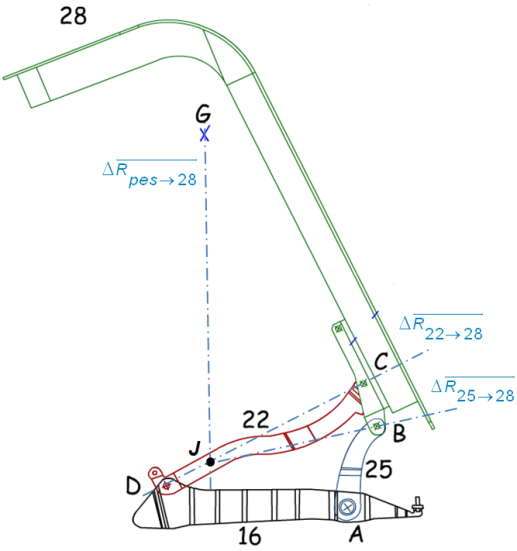
\includegraphics[width=2.34653in,height=2.50139in]{11-Actions Mécaniques/Cours/pandoc/media/image144.png}
\includegraphics{11-Actions Mécaniques/Cours/pandoc/media/image145.wmf}et 
\includegraphics{11-Actions Mécaniques/Cours/pandoc/media/image146.wmf}

On connait 
\includegraphics{11-Actions Mécaniques/Cours/pandoc/media/image147.wmf}, on peut donc trouver \emph{J} et en déduire~ 
\includegraphics{11-Actions Mécaniques/Cours/pandoc/media/image148.wmf}

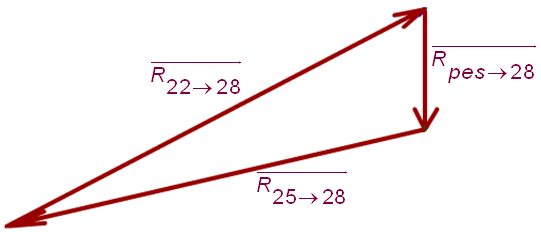
\includegraphics[width=2.75556in,height=1.18611in]{11-Actions Mécaniques/Cours/pandoc/media/image149.png}On connait 
\includegraphics{11-Actions Mécaniques/Cours/pandoc/media/image150.wmf}, on peut donc déterminer 
\includegraphics{11-Actions Mécaniques/Cours/pandoc/media/image151.wmf}

\begin{quote}
\textbf{\emph{Ces résultats, pour les ensembles isolés soumis à 2 ou 3 glisseurs, seront particulièrement utiles pour la RESOLUTION GRAPHIQUE de problèmes~!}}
\end{quote}

\hypertarget{section-1}{%
\subsubsection*{}\label{section-1}}
\addcontentsline{toc}{subsubsection}{}

\hypertarget{synthuxe8se-de-la-duxe9marche-de-ruxe9solution-dun-probluxe8me-duxe9quilibre}{%
\subsubsection{Synthèse de la démarche de résolution d'un problème d'équilibre}\label{synthuxe8se-de-la-duxe9marche-de-ruxe9solution-dun-probluxe8me-duxe9quilibre}}

Bien que chaque cas soit différent et que seule la pratique et la confrontation à de nombreuses situations différentes permettent de se préparer à faire face à des problématiques inédites, on peut proposer les démarches de résolution ci-dessous~:

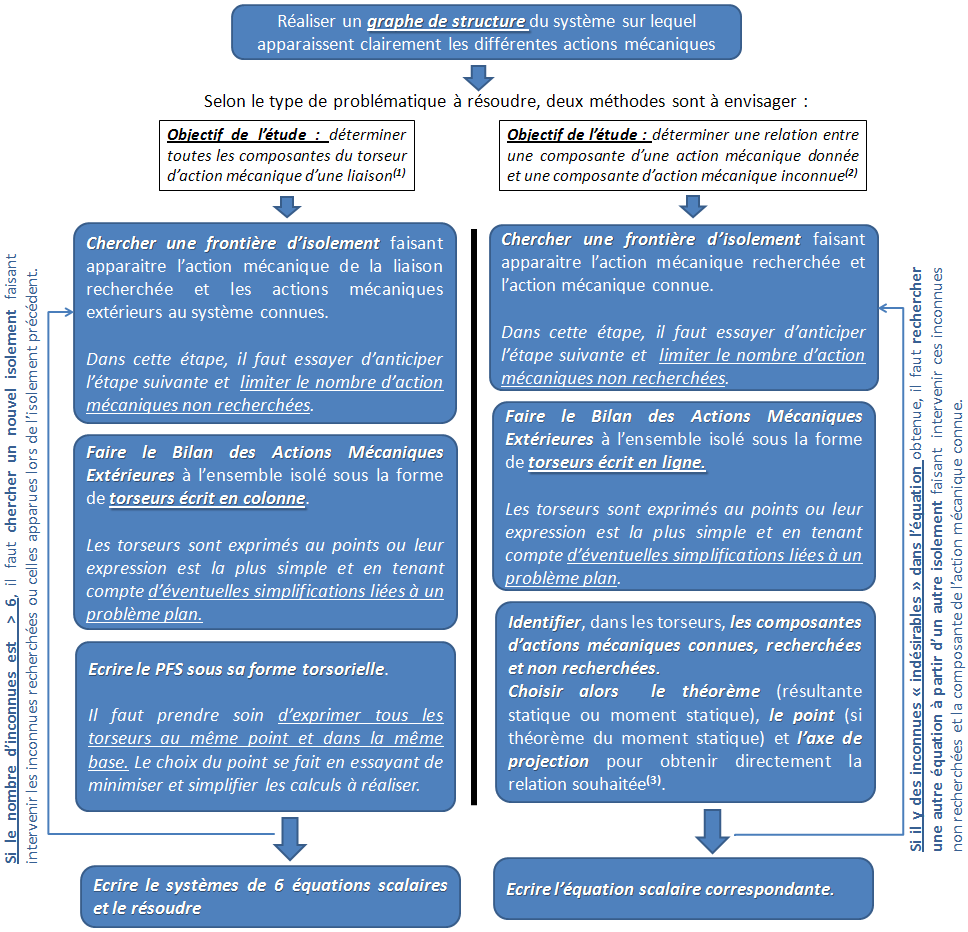
\includegraphics[width=6.36042in,height=6.24444in]{11-Actions Mécaniques/Cours/pandoc/media/image152.png}

\begin{longtable}[]{@{}
  >{\raggedright\arraybackslash}p{(\columnwidth - 0\tabcolsep) * \real{1.0000}}@{}}
\toprule\noalign{}
\begin{minipage}[b]{\linewidth}\raggedright
\begin{quote}
\textbf{\emph{\ul{Remarque~:}}}

\emph{Si, dans le cas d'un \textbf{problème plan}, le bilan des actions mécaniques extérieures à un ensemble isolé fait apparaître \textbf{2 ou 3 torseurs glisseurs}, on peut alors imaginer une \textbf{traduction graphique de l'équilibre} pour obtenir une valeur approchée de la norme de l'action mécanique recherchée à partir de l'action mécanique connue.}
\end{quote}
\end{minipage} \\
\midrule\noalign{}
\endhead
\bottomrule\noalign{}
\endlastfoot
 \\
\end{longtable}

\begin{longtable}[]{@{}
  >{\raggedright\arraybackslash}p{(\columnwidth - 2\tabcolsep) * \real{0.1111}}
  >{\raggedright\arraybackslash}p{(\columnwidth - 2\tabcolsep) * \real{0.8750}}@{}}
\toprule\noalign{}
\begin{minipage}[b]{\linewidth}\raggedright
\begin{quote}
\includegraphics{1 1-Act ions Mécan iques /Cour s/pan doc/m edia/ image 8.png}\{wid th=``0 .6262 69685 03937 01in''

heigh t=``0. 65083 33333 33333 4in''\}
\end{quote}
\end{minipage} & \begin{minipage}[b]{\linewidth}\raggedright
\textbf{Console de Bateau}

\begin{longtable}[]{@{}
  >{\raggedright\arraybackslash}p{(\columnwidth - 4\tabcolsep) * \real{0.1944}}
  >{\raggedright\arraybackslash}p{(\columnwidth - 4\tabcolsep) * \real{0.2222}}
  >{\raggedright\arraybackslash}p{(\columnwidth - 4\tabcolsep) * \real{0.3611}}@{}}
\toprule\noalign{}
\begin{minipage}[b]{\linewidth}\raggedright
\emph{\textbf{{[}Pr oblématique 1~:{]}\{.u nderline\}} Déterminer, connaissant l'effort} {[}{]} (11-Actions Mécaniques /Cours/pand oc/media/im age153.wmf) \emph{développé} \emph{par le vérin pour maintenir la barre en équilibre, les AM transmises par les liaisons en A\textsubscript{1} et A\textsubscript{2} (en vue du dime nsionnement des roulements à billes)}
\end{minipage} & \begin{minipage}[b]{\linewidth}\raggedright
\end{minipage} & \begin{minipage}[b]{\linewidth}\raggedright
\emph{\textbf{\ul{Problématique 2~:}} Déterminer l'effort} 
\includegraphics{11-Actio ns Mécaniques/Cours/pan doc/media/image154.wmf} \emph{que doit développer le vérin hydraulique pour maintenir la barre en équilibre sous l'action de l'eau sur le safran.}
\end{minipage} \\
\midrule\noalign{}
\endhead
\bottomrule\noalign{}
\endlastfoot
Pour ces deux pro blématiques d ifférentes, c'est le même isolement qui permet de faire apparaitre les actions mécaniques connues et celles re cherchées~: & \includegraphics{11-Act ions Mécaniqu es/Cours/pand oc/media/imag e155.png}\{wid th=``3.9375in'' heig ht=``1.5659142 607174104in''\} & \\
BAME à 1~:

Action de {[}{]} (11-Actions Mécaniques /Cours/pand oc/media/im age156.wmf) Action de {[}{]} (11-Actions Mécaniques /Cours/pand oc/media/im age157.wmf)

Action de {[}{]} (11-Actions Mécaniques /Cours/pand oc/media/im age158.wmf) Action de {[}{]} (11-Actions Mécaniques /Cours/pand oc/media/im age159.wmf)

Action de {[}{]} (11-Actions Mécaniques /Cours/pand oc/media/im age160.wmf)

Sous forme de torseurs écris \textbf{{[}en co lonne{]}\{.und erline\}}~:

\includegraphics{11 -Actions Mé caniques/Co urs/pandoc/ media/image 161.wmf}{[}{]} (11-Actions Mécaniques /Cours/pand oc/media/im age162.wmf)

\includegraphics{11 -Actions Mé caniques/Co urs/pandoc/ media/image 163.wmf}{[}{]} (11-Actions Mécaniques /Cours/pand oc/media/im age164.wmf)

{[}{]} (11-Actions Mécaniques /Cours/pand oc/media/im age165.wmf)

Pour traduire cette équation torsorielle en équations scalaires, il faut exprimer les différents torseurs au même point et dans la même base.

En choisissant le point A\textsubscript{1}, on évite d'avoir à déplacer le torseur dont la résultante est la plus «~lourde~».

{[}{]} (11-Actions Mécaniques /Cours/pand oc/media/im age167.wmf)

\includegraphics{11-Ac tions Mécan iques/Cours /pandoc/med ia/image168 .wmf}\includegraphics{11 -Actions Mé caniques/Co urs/pandoc/ media/image 169.wmf}{[}{]} (11-Actions Mécaniques /Cours/pand oc/media/im age170.wmf) & & BAME à 1~:

Action de 
\includegraphics{11-Actio ns Mécaniques/Cours/pan doc/media/image156.wmf} Action de
\includegraphics{11-Actio ns Mécaniques/Cours/pan doc/media/image157.wmf}

Action de 
\includegraphics{11-Actio ns Mécaniques/Cours/pan doc/media/image158.wmf} Action de 
\includegraphics{11-Actio ns Mécaniques/Cours/pan doc/media/image159.wmf}

Action de 
\includegraphics{11-Actio ns Mécaniques/Cours/pan doc/media/image160.wmf}

Sous forme de torseurs écris \textbf{\ul{en ligne}}~:


\includegraphics{11-Actio ns Mécaniques/Cours/pan doc/media/image171.wmf}


\includegraphics{11-Actio ns Mécaniques/Cours/pan doc/media/image172.wmf}


\includegraphics{11-Actio ns Mécaniques/Cours/pan doc/media/image174.wmf}


\includegraphics{11-Actio ns Mécaniques/Cours/pan doc/media/image175.wmf}


\includegraphics{11-Actio ns Mécaniques/Cours/pan doc/media/image176.wmf}

\textbf{\emph{\ul{Théorème du moment statique au point A\textsubscript{1} projeté sur l'axe}}} 
\includegraphics{11-Actions M écaniques/Cours/pandoc/ media/image177.wmf}\emph{~:} 
\includegraphics{11-Actio ns Mécaniques/Cours/pan doc/media/image178.wmf}


\includegraphics{11-Actions Mécaniques/Cours/pandoc /media/image179.wmf}Sur les calculs détaillés sur l'exemple de droite, on voit que de tous les produits vectoriels qui font apparaître 
\includegraphics{11-Actions M écaniques/Cours/pandoc/ media/image177.wmf}vont être 
\includegraphics{11-Actions Mécaniques/Cours/pandoc /media/image180.wmf}\emph{à} 
\includegraphics{11-Actions Mécaniques/Cours/pandoc /media/image177.wmf}\emph{.}


\includegraphics{11-Actio ns Mécaniques/Cours/pan doc/media/image181.wmf} \\
Ce qui nous donne~:

\includegraphics{11-Ac tions Mécan iques/Cours /pandoc/med ia/image182 .wmf}\includegraphics{11 -Actions Mé caniques/Co urs/pandoc/ media/image 183.wmf}{[}{]} (11-Actions Mécaniques /Cours/pand oc/media/im age184.wmf)

\includegraphics{11 -Actions Mé caniques/Co urs/pandoc/ media/image 185.wmf}{[}{]} (11-Actions Mécaniques /Cours/pand oc/media/im age186.wmf) & & \\
\end{longtable}
\end{minipage} \\
\midrule\noalign{}
\endhead
\bottomrule\noalign{}
\endlastfoot
& \\
\end{longtable}

\begin{longtable}[]{@{}
  >{\raggedright\arraybackslash}p{(\columnwidth - 2\tabcolsep) * \real{0.1111}}
  >{\raggedright\arraybackslash}p{(\columnwidth - 2\tabcolsep) * \real{0.8750}}@{}}
\toprule\noalign{}
\begin{minipage}[b]{\linewidth}\raggedright
\begin{quote}
\includegraphics{1 1-Act ions Mécan iques /Cour s/pan doc/m edia/ image 8.png}\{wid th=``0 .6262 69685 03937 01in''

heigh t=``0. 65083 33333 33333 4in''\}
\end{quote}
\end{minipage} & \begin{minipage}[b]{\linewidth}\raggedright

\includegraphics[width=2.5in,height=1.925in]{11-Actio ns Mécaniques/Cours/pandoc/media/image17.jpeg}\textbf{Poussoir et coulisseau}

On associe les repères~:

\begin{quote}
- \(R_{0}(O,\overset{\rightarrow}{x_{0}} ,\overset{\rightarrow}{y_{0}},\overset{\rightarrow}{z_{0}})\) au bâti 0, tel que

\(\overset{\rightarrow}{OB} = b.\overset{\rightarrow}{x_{0}}\)

- \(R_{1}(O,\overset{\rightarrow}{x_{1}} ,\overset{\rightarrow}{y_{1}},\overset{\rightarrow}{z_{1}})\) au poussoir 1, tels que

\(\over set{\rightarrow}{BA} = \lambda.\overset{\rightarrow}{y_{0}}\) et \(\alpha = (\overset{\rightarrow}{x_{0}},\overset{\rightarrow}{x_{1}})\)
\end{quote}

Un système non représenté assure le maintien du contact du coulisseau 2 avec le poussoir 1 au point A.

Le poussoir 1 est soumis au couple moteur \(C_{m}\) et le piston 2 à l'action 
\includegraphics{11-Actions Mécaniques/Cours/pandoc/media/image18.wmf} de pression du fluide.

On suppose le problème plan, les liaisons sans frottement et on néglige les effets d'inertie et de la pesanteur.

\textbf{L'objectif de l'étude est de déterminer une relation entre F et} \(\mathbf{C}_{\mathbf{m}}\) \textbf{lorsque le système est en équilibre.}

\textbf{Déterminer une relation entre le couple moteur} \(\mathbf{C}_{\mathbf{m}}\) \textbf{et l'effort} \(\mathbf{F}\)\textbf{.}
\end{minipage} \\
\midrule\noalign{}
\endhead
\bottomrule\noalign{}
\endlastfoot
& \\
\end{longtable}

\hypertarget{duxe9finir-une-action-muxe9canique-point-de-vue-local}{%
\subsection{Définir une action mécanique~: Point de vue local}\label{duxe9finir-une-action-muxe9canique-point-de-vue-local}}

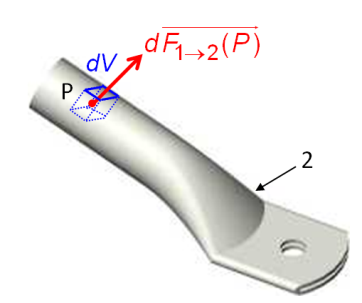
\includegraphics[width=1.64861in,height=1.37708in]{11-Actions Mécaniques/Cours/pandoc/media/image187.png}L'action mécanique d'un élément 1 sur un solide 2 (AM de 
\includegraphics{11-Actions Mécaniques/Cours/pandoc/media/image188.wmf}) est répartie sur la surface (action de contact) ou sur le volume (action à distance) du solide 2.

Soit P, un point appartenant à 2 et concerné par cette action mécanique. On définit localement une \textbf{force élémentaire} \(d\overrightarrow{F_{1 \rightarrow 2}(P)}\) agissant sur une surface ou un volume de dimension réduite définie au voisinage de P.

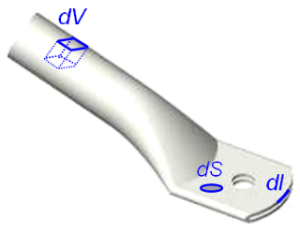
\includegraphics[width=1.36111in,height=1.05347in]{11-Actions Mécaniques/Cours/pandoc/media/image189.png}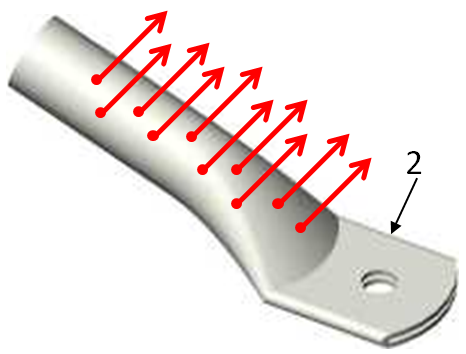
\includegraphics[width=1.86111in,height=1.41042in]{11-Actions Mécaniques/Cours/pandoc/media/image190.png}

L'expression de cette force élémentaire \(d\overrightarrow{F_{1 \rightarrow 2}(P)}\) varie en fonction de la nature de l'élément de 2 associé à P~:

\begin{longtable}[]{@{}
  >{\raggedright\arraybackslash}p{(\columnwidth - 8\tabcolsep) * \real{0.0735}}
  >{\raggedright\arraybackslash}p{(\columnwidth - 8\tabcolsep) * \real{0.0686}}
  >{\raggedright\arraybackslash}p{(\columnwidth - 8\tabcolsep) * \real{0.1127}}
  >{\raggedright\arraybackslash}p{(\columnwidth - 8\tabcolsep) * \real{0.3382}}
  >{\raggedright\arraybackslash}p{(\columnwidth - 8\tabcolsep) * \real{0.3971}}@{}}
\toprule\noalign{}
\begin{minipage}[b]{\linewidth}\raggedright
\textbf{\emph{Nature de l'élément}}
\end{minipage} & \begin{minipage}[b]{\linewidth}\raggedright
\textbf{\emph{Elément géométrique associé}}
\end{minipage} & \begin{minipage}[b]{\linewidth}\raggedright
\textbf{\emph{Densité de l'action mécanique}}
\end{minipage} & \begin{minipage}[b]{\linewidth}\raggedright
\textbf{\emph{unité}}
\end{minipage} & \begin{minipage}[b]{\linewidth}\raggedright
\textbf{\emph{Expression de}} \(\mathbf{d}\overrightarrow{\mathbf{F}_{\mathbf{1 \rightarrow 2}}\mathbf{(P)}}\)
\end{minipage} \\
\midrule\noalign{}
\endhead
\bottomrule\noalign{}
\endlastfoot
\emph{Ligne} & \(dl\) & \emph{linéique} \(\overrightarrow{q}\) & \(\left\lbrack N \cdot m^{- 1} \right\rbrack\) & \(\overrightarrow{q} \cdot dl\) \\
\emph{Surface} & \(ds\) & \emph{surfacique} \(\overrightarrow{q}\) & \(\left\lbrack N \cdot m^{- 2} \right\rbrack ou\lbrack Pa\rbrack\) & \(\overrightarrow{q} \cdot ds\) \\
\emph{Volume} & \(dv\) & \emph{volumique} \(\overrightarrow{q}\) & \(\left\lbrack N \cdot m^{- 3} \right\rbrack\) & \(\overrightarrow{q} \cdot dv\) \\
\end{longtable}

L'ensemble des forces élémentaires agissant sur l'ensemble des éléments concerné par l'action mécanique est appelé \textbf{\emph{champ de forces}} associé à l'action mécanique.

C'est la connaissance de ce champ de forces qui va permettre d'étudier les déformations. d'un solide soumis à une action mécanique.

\hypertarget{duxe9finir-une-action-muxe9canique-du-point-de-vue-local-au-point-de-vue-global}{%
\subsubsection{Définir une action mécanique~: du point de vue local au point de vue global}\label{duxe9finir-une-action-muxe9canique-du-point-de-vue-local-au-point-de-vue-global}}

Pour étudier le comportement des systèmes, on fait l'hypothèse que les pièces qui le constituent sont indéformables (sauf les pièces dont le but est de se déformer, ressorts,\ldots). Dans ce cas, on peut utiliser un \textbf{\emph{modèle global}} des actions mécaniques.

Si on reprend le cas d'un solide 2 soumis à l'action mécanique d'un élément 1, cela revient à considérer que ce dernier exerce sur le solide 2 une force \(\overrightarrow{F_{1 \rightarrow 2}}\) tel que~:


\includegraphics{11-Actions Mécaniques/Cours/pandoc/media/image191.wmf} \emph{Z} est la zone du solide 2 sur laquelle s'exerce l'AM de 
\includegraphics{11-Actions Mécaniques/Cours/pandoc/media/image188.wmf}

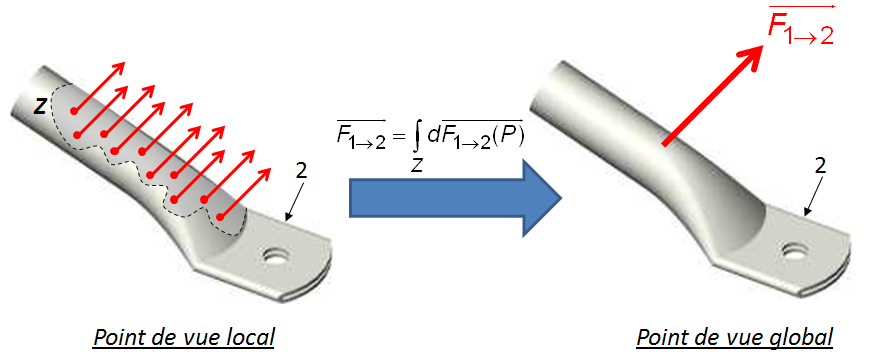
\includegraphics[width=4.35in,height=1.75973in]{11-Actions Mécaniques/Cours/pandoc/media/image192.png}

\hypertarget{torseur-des-actions-muxe9caniques}{%
\subsubsection{Torseur des actions mécaniques}\label{torseur-des-actions-muxe9caniques}}

\begin{itemize}
\tightlist
\item
  \textbf{\ul{Résultante de l'action mécanique}}
\end{itemize}

La résultante de l'action mécanique de \(1 \rightarrow 2\), notée \(\overrightarrow{R_{1 \rightarrow 2}}\) correspond à l'action mécanique globale créée par toutes contributions \(d\overrightarrow{F_{1 \rightarrow 2}(P)}\) du champ de forces élémentaires. On a donc~:


\includegraphics{11-Actions Mécaniques/Cours/pandoc/media/image193.wmf} \emph{(Newton~: N)}

Mais cette notion de résultante ne suffit pas pour caractériser correctement l'effet de cette action mécanique sur le solide 2. En effet, on s'intéresse à la façon dont cette action mécanique va provoquer, modifier ou empêcher le mouvement du solide 2.

\textbf{\emph{\ul{Exemple~:}}}

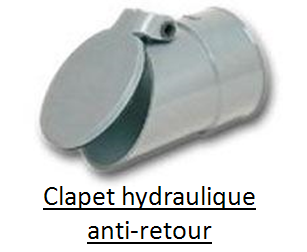
\includegraphics[width=1.37292in,height=1.26319in]{11-Actions Mécaniques/Cours/pandoc/media/image194.png}Pour les deux montages des clapets anti-retour schématisés ci-dessous, la résultante \(\overrightarrow{R_{2 \rightarrow 1}}\) de l'action mécanique de l'eau 2 sur le clapet 1 est la même.

Pour autant, le mouvement du clapet engendré par cette action mécanique sera différent d'un montage à l'autre~:

\begin{itemize}
\item
  rotation de centre A dans le sens horaire (montage 1)~;
\item
  rotation de centre B dans le sens anti-horaire (montage 2).
\end{itemize}

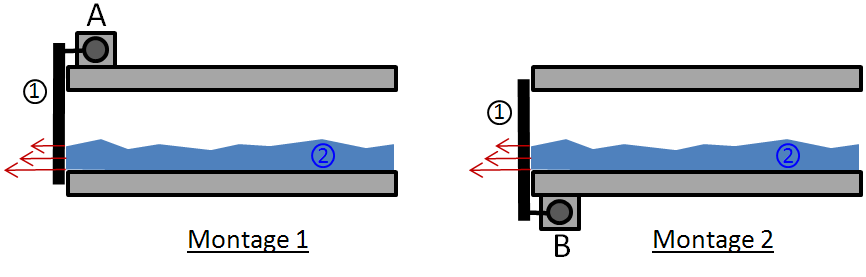
\includegraphics[width=4.47761in,height=1.32836in]{11-Actions Mécaniques/Cours/pandoc/media/image195.png}

Pour caractériser cette différence on utilise la notion de \textbf{\emph{moment résultant}}.

\begin{itemize}
\tightlist
\item
  \textbf{\ul{Moment Résultant de l'action mécanique}}
\end{itemize}

Le moment résultant de l'action mécanique de 
\includegraphics{11-Actions Mécaniques/Cours/pandoc/media/image188.wmf}, exprimé en un point J fixe, est un vecteur qui permet de «~caractériser~» la capacité de cette action mécanique à provoquer, à modifier ou à empêcher un mouvement de rotation du solide 2 autour de ce point J. Il est défini par~:


\includegraphics{11-Actions Mécaniques/Cours/pandoc/media/image196.wmf} \textbf{\emph{(Newton. mètre~: N.m)}}

\emph{Z} est la zone du solide 2 sur laquelle s'exerce l'AM de 
\includegraphics{11-Actions Mécaniques/Cours/pandoc/media/image188.wmf}

\textbf{\ul{Torseur de l'action mécanique}}

Pour faire le bilan des effets d'une action mécanique 1 agissant sur un solide 2, on utilise le torseur suivant~: 
\includegraphics{11-Actions Mécaniques/Cours/pandoc/media/image197.wmf}

On appelle «~\textbf{\emph{éléments de réduction}}~» du torseur, au point J, de l'AM de 
\includegraphics{11-Actions Mécaniques/Cours/pandoc/media/image188.wmf} :

\begin{itemize}
\item
  La \textbf{\emph{\ul{résultante}}} de l'AM de \textgreater{} 
\includegraphics{11-Actions Mécaniques/Cours/pandoc/media/image188.wmf}~: \textgreater{} 
\includegraphics{11-Actions Mécaniques/Cours/pandoc/media/image198.wmf}\emph{.} \textgreater{} \ul{Elle est indépendante du point d'expression du \textgreater{} torseur.}
\item
  Le \textbf{\emph{\ul{moment résultant}}} de l'AM de \textgreater{} 
\includegraphics{11-Actions Mécaniques/Cours/pandoc/media/image188.wmf}~ : \textgreater{} 
\includegraphics{11-Actions Mécaniques/Cours/pandoc/media/image199.wmf}\emph{.} \ul{Il \textgreater{} dépend du point d'expression du torseur.}
\end{itemize}

\textbf{\emph{\ul{Remarque~:}}} le moment vérifie la relation du champ des moments d'un torseur (Varignon)~:


\includegraphics{11-Actions Mécaniques/Cours/pandoc/media/image200.wmf} de l'espace 
\includegraphics{11-Actions Mécaniques/Cours/pandoc/media/image201.wmf}

\textbf{Lorsqu'on déplace un torseur d'un point à un autre on utilisera cette relation. On dit qu'on réduit le torseur (question~: Réduire le torseur, ou trouver les éléments de réduction,\ldots)}

\begin{longtable}[]{@{}
  >{\raggedright\arraybackslash}p{(\columnwidth - 2\tabcolsep) * \real{0.1111}}
  >{\raggedright\arraybackslash}p{(\columnwidth - 2\tabcolsep) * \real{0.8750}}@{}}
\toprule\noalign{}
\begin{minipage}[b]{\linewidth}\raggedright
\begin{quote}
\includegraphics{1 1-Act ions Mécan iques /Cour s/pan doc/m edia/ image 8.png}\{wid th=``0 .6262 69685 03937 01in''

heigh t=``0. 65083 33333 33333 4in''\}
\end{quote}
\end{minipage} & \begin{minipage}[b]{\linewidth}\raggedright

\includegraphics[width=1.95625in,height=2.65in]{11-Actions Mé caniques/Cours/pandoc/media/image202.jpeg}\textbf{Piston}

\textbf{Déterminer l'action mécanique de l'air sur le piston, notée} \(\left\{ T_{p \rightarrow 8} \right\}_{A}\)

\[\left\{ T_{p \rightarrow 8} \right\}_{A} = \begin{Bmatrix}
\overrightarrow{R_{p \rightarrow 8}} \\
\overrightarrow{M_{A,p \rightarrow 8}}
\end{Bmatrix} = \begin{Bmatrix}
\int_{S}^{}\overrightarrow{dF_{p \rightarrow 8}(M)} \\
\int_{S}^{}{\overri
ghtarrow{AM} \land \overrightarrow{dF_{p \rightarrow 8}(M)}}
\end{Bmatrix}\]

\[\overrightarr
ow{R_{p \rightarrow 8}} = \int_{S}^{}\overrightarrow{dF_{p \
rightarrow 8}(M)} = \int_{S}^{}{p \cdot ds \cdot \overrighta
rrow{x}} = \int_{S}^{}{p \cdot r \cdot dr \cdot d\theta \cdo
t \overrightarrow{x}} = p \cdot S \cdot \overrightarrow{x}\]

\[ds = r \cdot d\theta \cdot dr\]

\[\overrightarrow{M_{A,p \rightarrow 8}} = \int_{S}^{}{
\overrightarrow{AM} \land \overrightarrow{dF_{p \rightarrow
8}(M)}} = \int_{S}^{}{(r \cdot \cos\theta \cdot \overrightar
row{z} + r \cdot \sin\theta \cdot \overrightarrow{y}) \land
p \cdot r \cdot dr \cdot d\theta \cdot \overrightarrow{x}}\]


\includegraphics{11-Actions Mécaniques/Cours/pandoc/media/image203.wmf}

\[= p\int_{S}^{}{r^{2} \cdot dr \cdot \cos\theta \cdot d\
theta \cdot \overrightarrow{y} - p\int_{S}^{}{r^{2} \cdot dr
 \cdot \sin\theta} \cdot d\theta \cdot \overrightarrow{z}}\]

\[= p \cdot \overrightarrow{y}\in
t_{0}^{R}{r^{2} \cdot dr}\int_{0}^{2\pi}{\cos\theta \cdot d\
theta} - p \cdot \overrightarrow{z} \cdot \int_{0}^{R}{r^{2}
 \cdot dr} \cdot \int_{0}^{2\pi}{\sin\theta \cdot d\theta}\]

\[= p \cdot \overrightarrow{y}\left
\lbrack \frac{r^{3}}{3} \right\rbrack_{0}^{R}\left\lbrack \s
in\theta \right\rbrack_{0}^{2\pi} + p \cdot \overrightarrow{
z} \cdot \left\lbrack \frac{r^{3}}{3} \right\rbrack_{0}^{R}
\cdot \left\lbrack \cos\theta \right\rbrack_{0}^{2\pi} = 0\]
\end{minipage} \\
\midrule\noalign{}
\endhead
\bottomrule\noalign{}
\endlastfoot
& \\
\end{longtable}

\begin{longtable}[]{@{}
  >{\raggedright\arraybackslash}p{(\columnwidth - 2\tabcolsep) * \real{0.1111}}
  >{\raggedright\arraybackslash}p{(\columnwidth - 2\tabcolsep) * \real{0.8750}}@{}}
\toprule\noalign{}
\begin{minipage}[b]{\linewidth}\raggedright
\begin{quote}
\includegraphics{1 1-Act ions Mécan iques /Cour s/pan doc/m edia/ image 8.png}\{wid th=``0 .6262 69685 03937 01in''

heigh t=``0. 65083 33333 33333 4in''\}
\end{quote}
\end{minipage} & \begin{minipage}[b]{\linewidth}\raggedright
\textbf{Barrage}


\includegraphics[width=2.06528in,height=1.40556in]{11-Actions Mécaniques/Co urs/pandoc/media/image204.jpeg}Un barrage poids est un barrage dont la propre masse suffit à résister à la pression exercée par l\textquotesingle eau. Le barrage est soumis principalement à l'action mécanique de l'eau (pression hydrostatique) et à l'action mécanique de la pesanteur.

On s'intéresse à un barrage poids en béton de section triangulaire qui repose sur le sol et qui permet une retenue d'eau de hauteur h pour l'alimentation des voies navigables.

Le point O est situé dans le plan médian du barrage.


\includegraphics[width=3.02431in,height=2.06667in]{11-Actions Mécaniques/C ours/pandoc/media/image205.png}\ul{Les caractéristiques du barrage sont données ci-dessous~:}

m~: masse du barrage considéré comme un solide homogène.

a~= 20m : assise du barrage.

h = 25m~: hauteur d'eau.

L~= 80m : largeur du barrage.

ρ\textsubscript{eau} = 1000kg/m\textsuperscript{3}~: masse volumique de l'eau.

\textbf{L'effort maximal de poussée doit être de 300.10\textsuperscript{6} N.}

\textbf{Donner l'expression de la force élémentaire de pression de l'eau sur le barrage.}


\includegraphics[width=2.51319in,height=1.80833in]{11-Actions Mécaniques/C ours/pandoc/media/image206.png}\ul{Point de vue local~:}

Sur chaque élément de surface \(ds = dy \cdot dz\) situé autour d'un point Q de la paroi s'exerce un effort élémentaire~:

\[d\overrightarrow{F_{eau \righta
rrow barrage}(Q)} = p(Q) \cdot ds \cdot \overrightarrow{x}\]

Les lois de l'hydrostatique permettent d'écrire~: \(p(Q) = \rho_{eau} \cdot g \cdot (h - z)\)

On a donc~:

\[\boxed{d\overrig
htarrow{F_{eau \rightarrow barrage}(Q)} = \rho_{eau} \cdot g
 \cdot (h - z) \cdot dy \cdot dz \cdot \overrightarrow{x}}\]

\textbf{Déterminer les coordonnées du point} \(\mathbf{M(0,0,}\mathbf{z}_{\mathbf{M}}\mathbf{)}\) \textbf{ou le moment résultant de l'action mécanique de l'eau sur le barrage est nul. Donner, en ce point, l'expression du torseur de cette action mécanique.}

On cherche le point \(M(0,0,z_{M})\) pour lequel~: \(\overrig htarrow{M_{M,eau \rightarrow barrage}} = \overrightarrow{0}\)

Or~:

\[\overrightarrow{M_{M,eau \rig
htarrow barrage}} = \int_{S}^{}{\overrightarrow{MQ} \land}d\
overrightarrow{F_{eau \rightarrow barrage}(Q)} = \int_{S}^{}
{\left( \overrightarrow{MO} + \overrightarrow{OQ} \right) \l
and}\rho_{eau} \cdot g \cdot (h - z) \cdot dy \cdot dz \cdot
 \overrightarrow{x} = \int_{S}^{}{\left( \left( - z_{M} \cdo
t \overrightarrow{z} \right) + \left( y \cdot \overrightarro
w{y} + z \cdot \overrightarrow{z} \right) \right) \land}\rho
_{eau} \cdot g \cdot (h - z) \cdot dy \cdot dz \cdot \overri
ghtarrow{x} = \int_{S}^{}{- y \cdot \rho_{eau} \cdot g \cdot
 (h - z) \cdot dy \cdot dz \cdot \overrightarrow{z}} + \int_
{S}^{}{\left( z - z_{M} \right) \cdot \rho_{eau} \cdot g \cd
ot (h - z) \cdot dy \cdot dz \cdot \overrightarrow{y}} = 0\]

\[= - \rho
_{eau} \cdot g \cdot \overrightarrow{z} \cdot \int_{- \frac{
L}{2}}^{\frac{L}{2}}{y \cdot}dy \cdot \int_{0}^{h}{(h - z) \
cdot}dz + \rho_{eau} \cdot g \cdot \overrightarrow{y}\int_{0
}^{h}{(z - z_{M}) \cdot}(h - z) \cdot dz\int_{- \frac{L}{2}}
^{\frac{L}{2}} \cdot dy = \rho_{eau} \cdot g \cdot \overrigh
tarrow{z} \cdot \left\lbrack \frac{y^{2}}{2} \right\rbrack_{
- \frac{L}{2}}^{\frac{L}{2}} \cdot \left\lbrack h \cdot z -
\frac{z^{2}}{2} \right\rbrack_{0}^{h} + \rho_{eau} \cdot g \
cdot \overrightarrow{y} \cdot \left\lbrack (h + z_{M})\frac{
z^{2}}{2} - \frac{z^{3}}{3} - z \cdot z_{M} \cdot h \right\r
brack_{0}^{h} \cdot \lbrack y\rbrack_{- \frac{L}{2}}^{\frac{
L}{2}} = 0 + \rho_{eau} \cdot g \cdot \overrightarrow{y} \cd
ot (\frac{h^{3}}{6} - \frac{z_{M} \cdot h^{2}}{2}) \cdot L\]

Pour que \(\overrigh tarrow{M_{M,eau \rightarrow barrage}} = \overrightarrow{0}\), il faut donc que \(z_{M} = \frac{h}{3}\)

Au point M, le torseur de l'action mécanique de l'eau s'écrit~:

\[\l
eft\{ T_{eau \rightarrow barrage} \right\} = \begin{Bmatrix}
\overrightarrow{R_{eau \rightarrow barrage}} \\
\overrightarrow{0}
\end{Bmatrix}_{M}\]

Avec~:

\[\overrightarrow{R_{eau \
rightarrow barrage}} = \int_{S}^{}{d\overrightarrow{F_{eau \
rightarrow barrage}(Q)}} = \int_{S}^{}{\rho_{eau} \cdot g \c
dot (h - z) \cdot dy \cdot dz \cdot \overrightarrow{x}} = \r
ho_{eau} \cdot g \cdot \overrightarrow{x \cdot}\int_{0}^{h}{
(h - z) \cdot}dz\int_{- \frac{L}{2}}^{\frac{L}{2}}{dy} = \rh
o_{eau} \cdot g \cdot \overrightarrow{x} \cdot \left\lbrack
h \cdot z - \frac{z^{2}}{2} \right\rbrack_{0}^{h} \cdot \lbr
ack y\rbrack_{- \frac{L}{2}}^{\frac{L}{2}} = \rho_{eau} \cdo
t g \cdot L \cdot \frac{h^{2}}{2} \cdot \overrightarrow{x}\]

\[\boxed{\l
eft\{ T_{eau \rightarrow barrage} \right\} = \begin{Bmatrix}
\rho_{eau} \cdot
 g \cdot L \cdot \frac{h^{2}}{2} \cdot \overrightarrow{x} \\
\overrightarrow{0}
\end{Bmatrix}_{M}}\]


\includegraphics[width=6.69792in,height=2.5in]{11-Actions Mécaniques/ Cours/pandoc/media/image207.png}

\textbf{Vérifier le critère de l'effort de poussée.}

\[\overrightarrow{\left\| R_{eau \rightarrow
 barrage} \right\|} = \rho_{eau} \cdot g \cdot L \cdot \frac
{h^{2}}{2} = \boxed{245 \cdot 10^{6}N} < 300 \cdot 10^{6}N\]

Le critère est donc respecté.
\end{minipage} \\
\midrule\noalign{}
\endhead
\bottomrule\noalign{}
\endlastfoot
& \\
\end{longtable}

\hypertarget{prise-en-compte-du-phuxe9nomuxe8ne-de-frottement}{%
\subsection{Prise en compte du phénomène de frottement}\label{prise-en-compte-du-phuxe9nomuxe8ne-de-frottement}}

\hypertarget{frottement-en-translation}{%
\subsubsection[Frottement en translation]{\texorpdfstring{\protect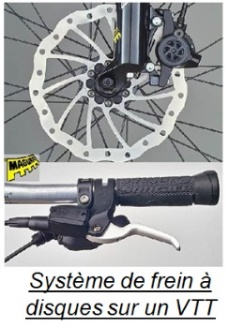
\includegraphics[width=1.04236in,height=1.48333in]{11-Actions Mécaniques/Cours/pandoc/media/image208.jpeg}Frottement en translation}{Frottement en translation}}\label{frottement-en-translation}}

Le phénomène de frottement est omniprésent dans l'étude du comportement et la conception des systèmes. Il peut être~:

\begin{itemize}
\item
  \textbf{\emph{utile}} lorsqu'il s'agit de freiner ou d'accélérer un solide~;
\item
  \textbf{\emph{néfaste}} lorsqu'il est à l'origine de pertes d'énergie ou d'usures trop importantes~;
\item
  \textbf{\emph{négligeable}} dans la plupart des cas.
\end{itemize}

On différencie deux cas~:

\begin{longtable}[]{@{}
  >{\raggedright\arraybackslash}p{(\columnwidth - 2\tabcolsep) * \real{0.2917}}
  >{\raggedright\arraybackslash}p{(\columnwidth - 2\tabcolsep) * \real{0.6944}}@{}}
\toprule\noalign{}
\begin{minipage}[b]{\linewidth}\raggedright
\textbf{FROTTEMENT}

entre 2 solides en contact
\end{minipage} & \begin{minipage}[b]{\linewidth}\raggedright
\emph{Il existe un mouvement relatif entre les 2 solides}
\end{minipage} \\
\midrule\noalign{}
\endhead
\bottomrule\noalign{}
\endlastfoot
\textbf{ADHERENCE}

entre 2 solides en contact & \emph{Il existe une tendance au mouvement mais il n'y a pas de mouvement relatif entre les 2 solides.} \\
\end{longtable}

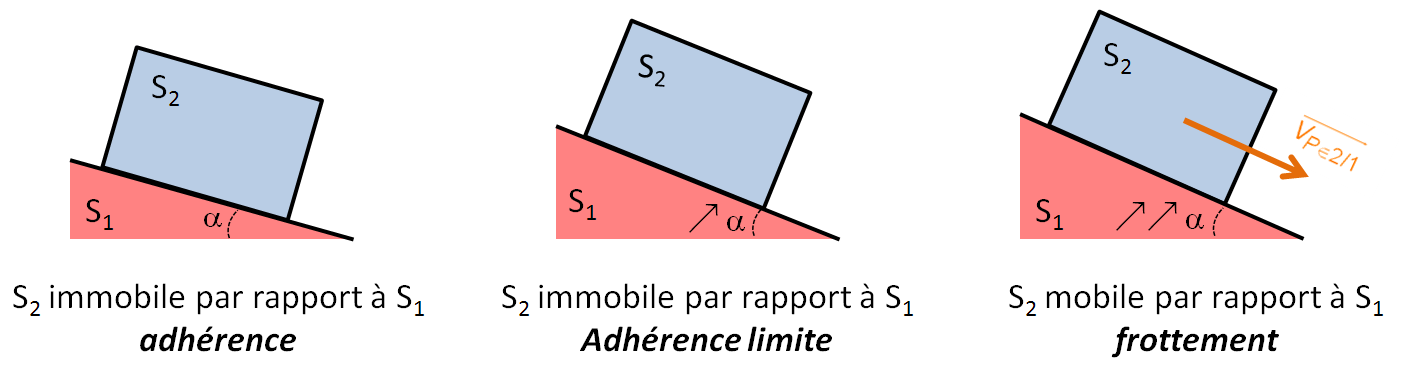
\includegraphics[width=4.69236in,height=1.24167in]{11-Actions Mécaniques/Cours/pandoc/media/image209.png}On peut illustrer cela avec l'exemple d'un colis S\textsubscript{2} posé sur un plan incliné~S\textsubscript{1} :

A partir d'une valeur limite de l'angle d'inclinaison 
\includegraphics{11-Actions Mécaniques/Cours/pandoc/media/image210.wmf}, il y perte d'adhérence entre S\textsubscript{2} et S\textsubscript{1}. Il y a alors apparition d'un mouvement relatif avec frottement de S\textsubscript{2} par rapport à S\textsubscript{1}.

\begin{longtable}[]{@{}
  >{\raggedright\arraybackslash}p{(\columnwidth - 6\tabcolsep) * \real{0.1806}}
  >{\raggedright\arraybackslash}p{(\columnwidth - 6\tabcolsep) * \real{0.2361}}
  >{\raggedright\arraybackslash}p{(\columnwidth - 6\tabcolsep) * \real{0.2500}}
  >{\raggedright\arraybackslash}p{(\columnwidth - 6\tabcolsep) * \real{0.3056}}@{}}
\toprule\noalign{}
\begin{minipage}[b]{\linewidth}\raggedright
\textbf{Mise en évidence des phénomènes de frottement et d'a dhérence}
\end{minipage} & \begin{minipage}[b]{\linewidth}\raggedright
\end{minipage} & \begin{minipage}[b]{\linewidth}\raggedright
\end{minipage} & \begin{minipage}[b]{\linewidth}\raggedright
\end{minipage} \\
\midrule\noalign{}
\endhead
\bottomrule\noalign{}
\endlastfoot
\emph{On prend l'exemple d'un colis S\textsubscript{2} posé sur un plan horizontal S\textsubscript{1}.} & & & \\
Le colis est au repos & Une action mécanique extérieure \(\over rightarrow{F}\) agit sur S\textsubscript{2} et tend à le faire glisser par rapport à S\textsubscript{1}. & & S\textsubscript{2} se met à glisser dans le même sens que \(\
overrightarrow{F}\). \\
\includegraphics{11-A ctions Méc aniques/Co urs/pandoc /media/ima ge211.wmf} & 
\includegraphics{11-Actions M écaniques/Cour s/pandoc/media /image212.wmf} & 
\includegraphics{11-Action s Mécaniques/Co urs/pandoc/medi a/image213.wmf} & ! \href{11-Actions\%20Mécan\%20iques/Cours/pandoc/\%20media/image214.wmf}{} \\
\includegraphics{11- Actions Mé caniques/C ours/pando c/media/im age215.png} & {[}{]} (11-Actions Mé caniques/Cours /pandoc/media/ image215.png)\{ width=``1.05833 33333333333in'' he ight=``1.348611 1111111112in''\} & \includegraphics{11-Actio ns Mécaniques/C ours/pandoc/med ia/image215.png} & \includegraphics{11-Acti ons Mécaniques/Cour s/pandoc/media/imag e215.png} \\
& Il existe une action tangentielle d'adhérence \(\overrigh tarrow{T_{a}}\) de S\textsubscript{2} sur S\textsubscript{1} (de même norme et de sens opposée à \(\overr ightarrow{F}\)) qui s'oppose à la tendance au mouvement relatif entre S\textsubscript{2} et S\textsubscript{1}.

Cette action tangentielle d'adhérence a une limite \(\overrightar row{T_{alim}}\) (égale et opposée à \(\overrightarr ow{F_{\lim}}\)) à partir de laquelle l'opposition à la tendance au mouvement ne sera plus suffisante pour maintenir S\textsubscript{2} immobile. & & Il existe une action tangentielle de frottement ! \href{11-Actions\%20Mécan\%20iques/Cours/pandoc/\%20media/image216.wmf}{} de S\textsubscript{2} sur S\textsubscript{1} (de norme constante et \textless{} \includegraphics{11-Actions Mécani ques/Cours/pandoc/m edia/image217.wmf}) qui s'oppose (sans l'empêcher) au glissement de S\textsubscript{2} par rapport à S\textsubscript{1}. \\
& \begin{minipage}[t]{\linewidth}\raggedright
\begin{itemize}
\tightlist
\item
  \textbf{ADHERENCE}*
\end{itemize}
\end{minipage} & \textbf{\emph{ADHERENCE LIMITE}} & \textbf{\emph{FROTTEMENT}} \\
\(\
overrighta rrow{P}\)~: résultante de l'action de la pesanteur sur S\textsubscript{2}

\(\
overrighta rrow{N}\)~: résultante des actions de pression de contact de S\textsubscript{1} sur S\textsubscript{2}

\(\
overrighta rrow{F}\)~: résultante de l'action extérieure agissant sur S\textsubscript{2} dans le but de le faire glisser sur S\textsubscript{1}

\(\over rightarrow {T_{a}}\)et \(\over rightarrow {T_{f}}\)~: r ésultantes des actions tan gentielles d 'adhérence et de frottement de S\textsubscript{1} sur S\textsubscript{2} & & & \\
\end{longtable}

Evolution de la résultante des actions tangentielles de frottement et d'adhérence~:

\begin{longtable}[]{@{}
  >{\raggedright\arraybackslash}p{(\columnwidth - 4\tabcolsep) * \real{0.2917}}
  >{\raggedright\arraybackslash}p{(\columnwidth - 4\tabcolsep) * \real{0.3333}}
  >{\raggedright\arraybackslash}p{(\columnwidth - 4\tabcolsep) * \real{0.3472}}@{}}
\toprule\noalign{}
\begin{minipage}[b]{\linewidth}\raggedright
\textbf{ADHERENCE}
\end{minipage} & \begin{minipage}[b]{\linewidth}\raggedright
\textbf{\emph{ADHERENCE LIMITE}}
\end{minipage} & \begin{minipage}[b]{\linewidth}\raggedright
\textbf{\emph{FROTTEMENT}}
\end{minipage} \\
\midrule\noalign{}
\endhead
\bottomrule\noalign{}
\endlastfoot
\(\overrighta
rrow{T_{a}} = - \o
verrightarrow{F}\) & \includegraphics{11-Actions M écaniques/Cours/pando c/media/image218.wmf} & \includegraphics{11-Actions Mécaniques/Cours/pand oc/media/image219.wmf} \\
angle d'adhérence \includegraphics{11-Actions Mécaniq ues/Cours/pandoc/m edia/image220.wmf} & angle d'adhérence \includegraphics{11-Actions M écaniques/Cours/pando c/media/image221.wmf} & angle de frottement \includegraphics{11-Actions Mécaniques/Cours/pand oc/media/image222.wmf} \\
\includegraphics{11-Actions Mécaniq ues/Cours/pandoc/m edia/image223.wmf} & \includegraphics{11-Actions M écaniques/Cours/pando c/media/image224.wmf}

\includegraphics{11-Actions Méca niques/Cours/pandoc/m edia/image225.wmf}est le \textbf{\emph{coefficient d'adhérence}} & \includegraphics{11-Actions Mécaniques/Cours/pand oc/media/image226.wmf}

\includegraphics{11-Actions Mécaniques/Cours/pand oc/media/image227.wmf} est le \textbf{\emph{coefficient de frottement}} \\
{[}{]} (11-Actions Mécani ques/Cours/pandoc/ media/image228.png )\{width=``2.6625in'' height=``1.43 05555555555556in''\} & & \\
\end{longtable}

\begin{itemize}
\tightlist
\item
  \textbf{\ul{Point de vue local~: loi de Coulomb}}
\end{itemize}

Soient deux solides 1 et 2 en contact sur une surface S et ayant une tendance au mouvement ou un mouvement relatif. La force élémentaire \includegraphics{11-Actions Mécaniques/Cours/pandoc/media/image229.wmf}de 1 sur 2 au point P se décompose en~:

\begin{itemize}
\item
  une \ul{\textbf{\emph{force élémentaire de pression}}} \includegraphics{11-Actions Mécaniques/Cours/pandoc/media/image230.wmf} normale au plan de contact (plan tangent commun aux deux solides)~;
\item
  une \textbf{\emph{\ul{force élémentaire tangentielle}}} \includegraphics{11-Actions Mécaniques/Cours/pandoc/media/image231.wmf} appartenant au plan de contact.
\end{itemize}

On a donc~: \includegraphics{11-Actions Mécaniques/Cours/pandoc/media/image232.wmf}

\begin{longtable}[]{@{}
  >{\raggedright\arraybackslash}p{(\columnwidth - 4\tabcolsep) * \real{0.3056}}
  >{\raggedright\arraybackslash}p{(\columnwidth - 4\tabcolsep) * \real{0.3333}}
  >{\raggedright\arraybackslash}p{(\columnwidth - 4\tabcolsep) * \real{0.3472}}@{}}
\toprule\noalign{}
\begin{minipage}[b]{\linewidth}\raggedright
\textbf{ADHERENCE}
\end{minipage} & \begin{minipage}[b]{\linewidth}\raggedright
\textbf{\emph{ADHERENCE LIMITE}}
\end{minipage} & \begin{minipage}[b]{\linewidth}\raggedright
\textbf{\emph{FROTTEMENT}}
\end{minipage} \\
\midrule\noalign{}
\endhead
\bottomrule\noalign{}
\endlastfoot
Vitesse de glissement! \href{11-Actions\%20Mécan\%20iques/Cours/pandoc/\%20media/image233.wmf}{} & Vitesse de gliss ement\includegraphics{11-Actions M écaniques/Cours/pando c/media/image233.wmf} & Vitesse de gl issement\includegraphics{11-Actions Mécaniques/Cours/pand oc/media/image234.wmf} \\
\includegraphics{11-Act ions Mécaniques/Cou rs/pandoc/media/ima ge235.png} & {[}{]} (11-Actions Mécanique s/Cours/pandoc/media/ image235.png)\{width='' 1.6932327209098863in'' height=``1 .5384612860892388in''\} & \includegraphics{11-Actions Mécani ques/Cours/pandoc/medi a/image235.png}\{width= ``1.5815562117235347in'' height='' 1.5512817147856517in''\} \\
! \href{11-Actions\%20Mécan\%20iques/Cours/pandoc/\%20media/image236.wmf}{} (angle d'adhérence) & \includegraphics{11-Actions M écaniques/Cours/pando c/media/image237.wmf} (angle d'adhérence limite) & \includegraphics{11-Actions Mécaniques/Cours/pand oc/media/image238.wmf} (angle de frottement) \\
! \href{11-Actions\%20Mécan\%20iques/Cours/pandoc/\%20media/image239.wmf}{}

Coef. d'adhérence ! \href{11-Actions\%20Mécan\%20iques/Cours/pandoc/\%20media/image240.wmf}{} & \includegraphics{11-Actions M écaniques/Cours/pando c/media/image241.wmf}

Coef. d'adhérence \includegraphics{11-Actions M écaniques/Cours/pando c/media/image240.wmf} & \includegraphics{11-Actions Mécaniques/Cours/pand oc/media/image242.wmf}

Coef. de frottement \includegraphics{11-Actions Mécaniques/Cours/pand oc/media/image243.wmf} \\
\includegraphics{11-Actions Mécaniqu es/Cours/pandoc/med ia/image244.wmf}est à \textbf{L'INTERIEUR} \textbf{du cône \ul{d'adhér ence}} & \includegraphics{11-Actions Méca niques/Cours/pandoc/m edia/image244.wmf}est \textbf{SUR} \textbf{le cône \ul{d'adh érence}} & \includegraphics{11-Actions Mé caniques/Cours/pandoc/ media/image244.wmf}est \textbf{SUR} \textbf{le cône de \ul{fro ttement}} \\
\(d\o verrightarrow{T_{1 \rightarrow 2}(P)}\) \textbf{\emph{s'oppose à la tendance au glissement}} \textbf{\emph{de 2/1.}} & \(d\overrightarrow{T_{ 1 \rightarrow 2}(P)}\) \textbf{\emph{s'oppose à la tendance au glissement de 2/1.}} & \(d\overrightarrow{T_ {1 \rightarrow 2}(P)}\) \textbf{\emph{s'oppose au glissement de 2/1.}} \(d\overright arrow{T_{1 \rightarrow  2}(P)} \land \overrig htarrow{V_{P \in 2/1}}  = \overrightarrow{0}\)

\(d\overrightarrow {T_{1 \rightarrow 2}(P )} \cdot \overrightarr ow{V_{P \in 2/1}} < 0\) \\
\end{longtable}

\begin{quote}
\textbf{Coefficients de frottement et d'adhérence~:} \includegraphics{11-Actions Mécaniques/Cours/pandoc/media/image245.wmf} \textbf{ou} \includegraphics{11-Actions Mécaniques/Cours/pandoc/media/image246.wmf}
\end{quote}

\includegraphics[width=2.55694in,height=1.51875in]{11-Actions Mécaniques/Cours/pandoc/media/image247.png}Le coefficient d'adhérence \includegraphics{11-Actions Mécaniques/Cours/pandoc/media/image248.wmf}est toujours légèrement supérieur au coefficient de frottement \includegraphics{11-Actions Mécaniques/Cours/pandoc/media/image249.wmf}(\includegraphics{11-Actions Mécaniques/Cours/pandoc/media/image250.wmf}).

On fera cependant, lors de l'étude du comportement statique et dynamique des systèmes, l'hypothèse simplificatrice qu'ils sont égaux. \textbf{\emph{On utilisera alors uniquement le coefficient de frottement que l'on notera}}~: \includegraphics{11-Actions Mécaniques/Cours/pandoc/media/image251.wmf} ou \includegraphics{11-Actions Mécaniques/Cours/pandoc/media/image252.wmf}\textbf{.}

\begin{longtable}[]{@{}
  >{\raggedright\arraybackslash}p{(\columnwidth - 2\tabcolsep) * \real{0.4722}}
  >{\raggedright\arraybackslash}p{(\columnwidth - 2\tabcolsep) * \real{0.5139}}@{}}
\toprule\noalign{}
\begin{minipage}[b]{\linewidth}\raggedright
La valeur de ce coefficient
\end{minipage} & \begin{minipage}[b]{\linewidth}\raggedright
\end{minipage} \\
\midrule\noalign{}
\endhead
\bottomrule\noalign{}
\endlastfoot
ne dépend pas\textbf{~:} & dépend essentiellement~: \\
\begin{minipage}[t]{\linewidth}\raggedright
\begin{itemize}
\item
  de l'intensité de la force élémentaire de pression~;
\item
  de l'étendue de la surface de contact.
\end{itemize}
\end{minipage} & \begin{minipage}[t]{\linewidth}\raggedright
\begin{itemize}
\item
  de la \textbf{nature des matériaux} \textgreater{} en contact~;
\item
  de la présence ou non de \textgreater{} \textbf{lubrifiant~};
\item
  de l'état de rugosité, \textgreater{} température,\ldots{}
\end{itemize}
\end{minipage} \\
\end{longtable}

\begin{longtable}[]{@{}
  >{\raggedright\arraybackslash}p{(\columnwidth - 4\tabcolsep) * \real{0.3067}}
  >{\raggedright\arraybackslash}p{(\columnwidth - 4\tabcolsep) * \real{0.2933}}
  >{\raggedright\arraybackslash}p{(\columnwidth - 4\tabcolsep) * \real{0.3733}}@{}}
\toprule\noalign{}
\begin{minipage}[b]{\linewidth}\raggedright
\textbf{matériaux} en contact
\end{minipage} & \begin{minipage}[b]{\linewidth}\raggedright
\textbf{f} ou \textbf{μ}
\end{minipage} & \begin{minipage}[b]{\linewidth}\raggedright
\end{minipage} \\
\midrule\noalign{}
\endhead
\bottomrule\noalign{}
\endlastfoot
& Surfaces \textbf{sèches} & Surfaces \textbf{lubrifiées} \\
\textbf{Acier/Acier} & \textbf{0.15} & \textbf{0.09} \\
\textbf{Acier/Fonte} & \textbf{0.16} & \textbf{0.08 à 0.04} \\
\textbf{Acier/Bronze} & \textbf{0.10} & \textbf{0.09} \\
\textbf{Téflon/Acier} & \textbf{0.04} & \textbf{-} \\
\textbf{Fonte/Bronze} & \textbf{0.20} & \textbf{0.08 à 0.04} \\
\textbf{Nylon/Acier} & \textbf{0.35} & \textbf{0.12} \\
\textbf{Bois/Bois} & \textbf{0.4 à 0.2} & \textbf{0.16 à 0.04} \\
\textbf{Pneu/Route} & \textbf{0.6} & \textbf{0.30 à 0.10} \\
\end{longtable}

\emph{\ul{Quelques ordres de grandeurs~de coefficient de frottement :}}

\begin{itemize}
\tightlist
\item
  \textbf{\ul{Point de vue local}}
\end{itemize}

Lors de la prise en compte du phénomène d'adhérence dans l'étude du comportement statique d'un système, \textbf{\emph{on se placera à la limite du glissement}} pour exprimer le torseur de l'action mécanique de 1 agissant sur 2~:

\includegraphics{11-Actions Mécaniques/Cours/pandoc/media/image253.wmf}

\emph{Ainsi on pourra utiliser l'équation qui lie} \includegraphics{11-Actions Mécaniques/Cours/pandoc/media/image254.wmf}\emph{(en général connu),} \includegraphics{11-Actions Mécaniques/Cours/pandoc/media/image255.wmf} et \includegraphics{11-Actions Mécaniques/Cours/pandoc/media/image256.wmf}~: \includegraphics{11-Actions Mécaniques/Cours/pandoc/media/image257.wmf}

En résumé~:

\begin{itemize}
\item
  L'existence d'un frottement dans une liaison implique qu'une composante nulle devient non nulle
\item
  L'effort tangentiel s'oppose toujours au mouvement
\item
  Pour modéliser l'AM, il faut isoler le solide en mouvement
\item
  Le cône de frottement se trouve toujours du côté du solide isolé
\item
  Le coefficient de frottement est positif et correspond au rapport de l'effort tangentiel et de l'effort normal~; on a~: \includegraphics{11-Actions Mécaniques/Cours/pandoc/media/image258.wmf}
\item
  L'angle \(\varphi\) correspond au demi-angle au sommet du cône.
\end{itemize}

\begin{longtable}[]{@{}
  >{\raggedright\arraybackslash}p{(\columnwidth - 2\tabcolsep) * \real{0.1111}}
  >{\raggedright\arraybackslash}p{(\columnwidth - 2\tabcolsep) * \real{0.8750}}@{}}
\toprule\noalign{}
\begin{minipage}[b]{\linewidth}\raggedright
\begin{quote}
\includegraphics{1 1-Act ions Mécan iques /Cour s/pan doc/m edia/ image 8.png}\{wid th=``0 .6262 69685 03937 01in''

heigh t=``0. 65083 33333 33333 4in''\}
\end{quote}
\end{minipage} & \begin{minipage}[b]{\linewidth}\raggedright
\textbf{Inclinaison}

\includegraphics[width=5.84292in,height=4.5995in]{11-Actions Mécaniques /Cours/pandoc/media/image259.png}

\textbf{Déterminer l'angle à partir duquel la caisse se met à glisser.}
\end{minipage} \\
\midrule\noalign{}
\endhead
\bottomrule\noalign{}
\endlastfoot
& \\
\end{longtable}

\begin{longtable}[]{@{}
  >{\raggedright\arraybackslash}p{(\columnwidth - 2\tabcolsep) * \real{0.1111}}
  >{\raggedright\arraybackslash}p{(\columnwidth - 2\tabcolsep) * \real{0.8750}}@{}}
\toprule\noalign{}
\begin{minipage}[b]{\linewidth}\raggedright
\begin{quote}
\includegraphics{1 1-Act ions Mécan iques /Cour s/pan doc/m edia/ image 8.png}\{wid th=``0 .6262 69685 03937 01in''

heigh t=``0. 65083 33333 33333 4in''\}
\end{quote}
\end{minipage} & \begin{minipage}[b]{\linewidth}\raggedright
\textbf{Collecteur de MCC}

\includegraphics[width=6.25347in,height=3.68681in]{11-Actions Mécaniques/C ours/pandoc/media/image260.jpeg}

\textbf{Déterminer l'angle à partir duquel la caisse se met à glisser.}

Le système représente un porte-balai de moteur à courant continu. Le levier sollicité par le ressort de traction appuie le charbon sur le collecteur pour faire le contact électrique. Pour un bon fonctionnement du moteur, l'effort presseur sur le collecteur doit être de 6 N.

La liaison charbon / collecteur au point E est assimilé à une liaison ponctuelle de normale \(\overrightarrow{y}\). avec frottement tel que \(\left\| \overright arrow{R_{collecteur \rightarrow charbon}} \right\| = \ 6\ N\) et f = 0,2.

\textbf{Exprimer le torseur de l'action du collecteur sur le charbon en E (calculer ses composantes).}
\end{minipage} \\
\midrule\noalign{}
\endhead
\bottomrule\noalign{}
\endlastfoot
& \\
\end{longtable}

\hypertarget{prise-en-compte-du-phuxe9nomuxe8ne-de-frottement-dans-une-liaison-pivot}{%
\subsubsection{Prise en compte du phénomène de frottement dans une liaison pivot}\label{prise-en-compte-du-phuxe9nomuxe8ne-de-frottement-dans-une-liaison-pivot}}

Dans le cas d'une liaison pivot, le frottement est modélisé par un torseur couple avec un couple de frottement (sec, visqueux ou fluide) qui est en général (par convention) affublé du signe «~-~».

\includegraphics{11-Actions Mécaniques/Cours/pandoc/media/image262.wmf}

\hypertarget{autres-phuxe9nomuxe8nes-de-frottements}{%
\subparagraph*{\texorpdfstring{\protect\includegraphics[width=2.59861in,height=1.93681in]{11-Actions Mécaniques/Cours/pandoc/media/image263.png}Autres phénomènes de frottements}{Autres phénomènes de frottements}}\label{autres-phuxe9nomuxe8nes-de-frottements}}
\addcontentsline{toc}{subparagraph}{Autres phénomènes de frottements}

\begin{itemize}
\tightlist
\item
  Résistance au pivotement
\end{itemize}

La résistance au pivotement est liée est un frottement qui apparait lorsqu'on essaye de faire pivoter deux surfaces l'une sur l'autre (comme un pneu sur le sol lorsqu'on est à l'arrêt). Elle se modélise par un moment perpendiculaire au plan tangent aux deux surfaces.

\begin{itemize}
\tightlist
\item
  Résistance au roulement
\end{itemize}

La résistance au roulement existe à partir du moment où on fait rouler un solide sur un autre solide. La pression de contact due à une surface très réduite (théoriquement ponctuelle ou linéaire) créé une déformation plus ou moins importante qui induit une perte d'énergie. Ce phénomène peut être modélisé par un torseur couple avec un moment qui tend à s'opposer au mouvement de rotation.

\includegraphics[width=6.5692in,height=2.49584in]{11-Actions Mécaniques/Cours/pandoc/media/image264.png}

\hypertarget{phuxe9nomuxe8ne-darc-boutement}{%
\subsubsection{Phénomène d'arc-boutement}\label{phuxe9nomuxe8ne-darc-boutement}}

\includegraphics[width=0.89514in,height=1.05694in]{11-Actions Mécaniques/Cours/pandoc/media/image265.png}On appelle arc-boutement, le phénomène issu de l'adhérence pour lequel un équilibre subsiste indépendamment de l'intensité de l'effort qui tend à le rompre.

\textbf{\ul{Exemple~:}} sur un serre-joint c'est le phénomène d'arc-boutement qui solidarise le mord mobile et le mord fixe après la 1\textsuperscript{ère} phase de réglage de l'écart entre les deux mords.

On peut aussi citer l'exemple du tiroir qui se bloque et les pinces de la cordeuse vue en TP.

\hypertarget{moment-dune-force-et-bras-de-levier}{%
\subsection[Moment d'une force et Bras de Levier]{\texorpdfstring{\protect\includegraphics[width=2.67292in,height=1.70278in]{11-Actions Mécaniques/Cours/pandoc/media/image266.jpeg}Moment d'une force et Bras de Levier}{Moment d'une force et Bras de Levier}}\label{moment-dune-force-et-bras-de-levier}}

Le moment d'une force par rapport à un point est un outil qui permet de mesurer la capacité de cette force à créer un mouvement de rotation autour de ce point ou à l'empêcher.

Soit un effort \includegraphics{11-Actions Mécaniques/Cours/pandoc/media/image267.wmf} appliqué au point Q. Le moment crée par cet effort au point P est un \textbf{vecteur} noté \({\overrightarrow{M}}_{P,\overrightarrow{F}}\)tel que :

\[{\overrightarrow{M}}_{P,\overrightarrow{F}} = \overrightarrow{PQ} \land \overrightarrow{F}\]

Si on prend la norme du moment de cette force, on dit que le moment est le produit de la force par le \textbf{bras de levier} (ici d=PH). Seule contrainte, le bras de levier doit être perpendiculaire à la force.

\[\left\| {\overrightarrow{M}}_{P,\overrightarrow{F}} \right\| = \overline{PH}\left\| \overrightarrow{F} \right\| = Fd\]

Dans le cas où le bras de levier et la force ne sont pas perpendiculaires, il faut faire des projections. Cela permet de vérifier les résultats rapidement dans le cas où on doit calculer les moments de glisseurs. En observant la tendance au mouvement de rotation il est aussi possible de déterminer le sens et la direction.

\begin{longtable}[]{@{}
  >{\raggedright\arraybackslash}p{(\columnwidth - 2\tabcolsep) * \real{0.1111}}
  >{\raggedright\arraybackslash}p{(\columnwidth - 2\tabcolsep) * \real{0.8750}}@{}}
\toprule\noalign{}
\begin{minipage}[b]{\linewidth}\raggedright
\begin{quote}
\includegraphics{1 1-Act ions Mécan iques /Cour s/pan doc/m edia/ image 8.png}\{wid th=``0 .6262 69685 03937 01in''

heigh t=``0. 65083 33333 33333 4in''\}
\end{quote}
\end{minipage} & \begin{minipage}[b]{\linewidth}\raggedright
\textbf{Bras de leviers 1}

\includegraphics[width=2.03333in,height=1.04722in]{11-Actions Mécaniques/ Cours/pandoc/media/image268.png}\includegraphics[width=1.98971in,height=1.08056in]{11-Actions Mécaniques/C ours/pandoc/media/image268.png}\includegraphics[width=1.85in,height=1.04722in]{11-Action s Mécaniques/Cours/pandoc/media/image268.png}

\textbf{Déterminer le moment en O pour les trois cas ci-dessus.}
\end{minipage} \\
\midrule\noalign{}
\endhead
\bottomrule\noalign{}
\endlastfoot
& \\
\end{longtable}

\begin{longtable}[]{@{}
  >{\raggedright\arraybackslash}p{(\columnwidth - 2\tabcolsep) * \real{0.1111}}
  >{\raggedright\arraybackslash}p{(\columnwidth - 2\tabcolsep) * \real{0.8750}}@{}}
\toprule\noalign{}
\begin{minipage}[b]{\linewidth}\raggedright
\begin{quote}
\includegraphics{1 1-Act ions Mécan iques /Cour s/pan doc/m edia/ image 8.png}\{wid th=``0 .6262 69685 03937 01in''

heigh t=``0. 65083 33333 33333 4in''\}
\end{quote}
\end{minipage} & \begin{minipage}[b]{\linewidth}\raggedright
\textbf{Bras de leviers 2}

\includegraphics[width=6.18347in,height=3.52432in]{11-Actions Mécaniques/ Cours/pandoc/media/image269.png}

\textbf{Calculer le moment résultant au niveau de l'axe de rotation situé au centre du disque. Ces disques sont-ils à l'équilibre~? Sinon, dans quel sens tourneront-ils~? Le rayon du disque est de 10 cm.}
\end{minipage} \\
\midrule\noalign{}
\endhead
\bottomrule\noalign{}
\endlastfoot
& \\
\end{longtable}

\begin{longtable}[]{@{}
  >{\raggedright\arraybackslash}p{(\columnwidth - 2\tabcolsep) * \real{0.1111}}
  >{\raggedright\arraybackslash}p{(\columnwidth - 2\tabcolsep) * \real{0.8750}}@{}}
\toprule\noalign{}
\begin{minipage}[b]{\linewidth}\raggedright
\begin{quote}
\includegraphics{1 1-Act ions Mécan iques /Cour s/pan doc/m edia/ image 8.png}\{wid th=``0 .6262 69685 03937 01in''

heigh t=``0. 65083 33333 33333 4in''\}
\end{quote}
\end{minipage} & \begin{minipage}[b]{\linewidth}\raggedright
\textbf{Vérin électrique}

Soit la modélisation d'un vérin électrique, en utilisant un modèle poutre~:

\includegraphics{11-Actions Mécaniques/Cours/pandoc/media/image270.png}

\textbf{Déterminer les moments en A pour chaque effort (F, Y\textsubscript{A}, X\textsubscript{A}, Y\textsubscript{B})}
\end{minipage} \\
\midrule\noalign{}
\endhead
\bottomrule\noalign{}
\endlastfoot
& \\
\end{longtable}

\begin{longtable}[]{@{}
  >{\raggedright\arraybackslash}p{(\columnwidth - 2\tabcolsep) * \real{0.1111}}
  >{\raggedright\arraybackslash}p{(\columnwidth - 2\tabcolsep) * \real{0.8750}}@{}}
\toprule\noalign{}
\begin{minipage}[b]{\linewidth}\raggedright
\begin{quote}
\includegraphics{1 1-Act ions Mécan iques /Cour s/pan doc/m edia/ image 8.png}\{wid th=``0 .6262 69685 03937 01in''

heigh t=``0. 65083 33333 33333 4in''\}
\end{quote}
\end{minipage} & \begin{minipage}[b]{\linewidth}\raggedright
\includegraphics[width=2.5in,height=1.925in]{11-Actio ns Mécaniques/Cours/pandoc/media/image17.jpeg}\textbf{Poussoir et coulisseau}

On associe les repères~:

\begin{quote}
- \(R_{0}(O,\overset{\rightarrow}{x_{0}} ,\overset{\rightarrow}{y_{0}},\overset{\rightarrow}{z_{0}})\) au bâti 0, tel que

\(\overset{\rightarrow}{OB} = b.\overset{\rightarrow}{x_{0}}\)

- \(R_{1}(O,\overset{\rightarrow}{x_{1}} ,\overset{\rightarrow}{y_{1}},\overset{\rightarrow}{z_{1}})\) au poussoir 1, tels que

\(\over set{\rightarrow}{BA} = \lambda.\overset{\rightarrow}{y_{0}}\) et \(\alpha = (\overset{\rightarrow}{x_{0}},\overset{\rightarrow}{x_{1}})\)
\end{quote}

\textbf{Déterminer} \(\overrightarrow{\mathbf{M}_{\mathbf{O,2 \rightarrow 1}}}\) \textbf{en utilisant le bras de levier}
\end{minipage} \\
\midrule\noalign{}
\endhead
\bottomrule\noalign{}
\endlastfoot
& \\
\end{longtable}

\begin{longtable}[]{@{}
  >{\raggedright\arraybackslash}p{(\columnwidth - 2\tabcolsep) * \real{0.1111}}
  >{\raggedright\arraybackslash}p{(\columnwidth - 2\tabcolsep) * \real{0.8750}}@{}}
\toprule\noalign{}
\begin{minipage}[b]{\linewidth}\raggedright
\begin{quote}
\includegraphics{1 1-Act ions Mécan iques /Cour s/pan doc/m edia/ image 8.png}\{wid th=``0 .6262 69685 03937 01in''

heigh t=``0. 65083 33333 33333 4in''\}
\end{quote}
\end{minipage} & \begin{minipage}[b]{\linewidth}\raggedright
\textbf{Console de bateaux}

Soit une console portante de bateaux.

\includegraphics[width=4.06667in,height=2.50833in]{11-Actions Mécaniques /Cours/pandoc/media/image3.jpeg}

\textbf{Déterminer la relation entre F3 et Fv en utilisant les bras de leviers pour calculer les moments au point A autour de l'axe z et en appliquant le théorème du moment statique. Les moments résultants en A des actions mécaniques en A, B et D sont nuls.}

\[e \cdot F_{V} - c \cdot F_{3} = 0\]

\[\Rightarrow F_{3} = \frac{e \cdot F_{V}}{c}\]
\end{minipage} \\
\midrule\noalign{}
\endhead
\bottomrule\noalign{}
\endlastfoot
& \\
\end{longtable}

\hypertarget{masse-centre-dinertie}{%
\subsection[Masse -- Centre d'inertie]{\texorpdfstring{\protect\includegraphics[width=2.75556in,height=1.78472in]{11-Actions Mécaniques/Cours/pandoc/media/image271.jpeg}Masse -- Centre d'inertie}{Masse -- Centre d'inertie}}\label{masse-centre-dinertie}}

\hypertarget{masse}{%
\subsubsection{Masse}\label{masse}}

Au point \textbf{P} d'un solide \textbf{S}, la masse \emph{dm} d'un petit élément de volume \emph{dv} s'exprime : \(dm = \rho.dv\)

\emph{La masse volumique, notée ρ est exprimée en kg/m\textsuperscript{3.}}

La masse du solide S est alors : \(M = \int_{S}^{}{dm} = \int_{S}^{}{\rho.dv}\)

Dans la plupart des cas, le matériau constituant le solide est homogène, on a donc : \(M = \rho.V\)

\emph{\ul{Quelques ordres de grandeurs (eau~: 1000 kg/m\textsuperscript{3})}}

\begin{longtable}[]{@{}
  >{\raggedright\arraybackslash}p{(\columnwidth - 2\tabcolsep) * \real{0.3514}}
  >{\raggedright\arraybackslash}p{(\columnwidth - 2\tabcolsep) * \real{0.6216}}@{}}
\toprule\noalign{}
\endhead
\bottomrule\noalign{}
\endlastfoot
matériau & Masse volumique \\
Acier & 7850 kg/m\textsuperscript{3} \\
Aluminium & 2700 kg/m\textsuperscript{3} \\
Fonte & 6800-7400 kg/m\textsuperscript{3} \\
\end{longtable}

\hypertarget{centre-dinertie}{%
\subsubsection{Centre d'inertie}\label{centre-dinertie}}

Le centre d'inertie d'un solide S est le barycentre G des masses élémentaires : \(\int_{S}^{}{\overrightarrow{GP}.dm = \overrightarrow{0}}\)

Soit un repère \(R(O,\overrightarrow{x},\overrightarrow{y},\overrightarrow{z})\) lié au solide S

\[\overrightarrow{GP} = \overrightarrow{GO} + \overrightarrow{OP}\]

On a donc :

\(\int_{S}^{}{\overrightarrow{GO}.dm + \int_{S}^{}{\overrightarrow{OP}.dm} = \overrightarrow{0}}\) \(\overrightarrow{GO}\int_{S}^{}{dm + \int_{S}^{}{\overrightarrow{OP}.dm} = \overrightarrow{0}}\)

Ce qui nous conduit à : \(\overrightarrow{OG} = \frac{1}{M}\int_{S}^{}{\overrightarrow{OP}.dm}\)

\textbf{Le centre d'inertie se situe sur les éléments de symétrie du solide (point, plan, droite)}

\includegraphics[width=2.20486in,height=1.42708in]{11-Actions Mécaniques/Cours/pandoc/media/image272.jpeg}

\textbf{Remarque}

Le centre de gravité d'un solide est le point d'application de la résultante des efforts de pesanteur.

On montre que :

\hypertarget{ensemble-de-solides}{%
\subparagraph*{Ensemble de solides}\label{ensemble-de-solides}}
\addcontentsline{toc}{subparagraph}{Ensemble de solides}

Le centre d'inertie d'un \textbf{ensemble Σ} de \textbf{n} \textbf{solides S\textsubscript{i}} , de \textbf{masse mi} et \textbf{centre d'inertie} \textbf{G\textsubscript{i}}, est \textbf{G\textsubscript{Σ}} tel que:

\(\overrightarrow{OG_{\Sigma}} = \frac{1}{M}\sum_{i = 1}^{n}{m_{i}.\overrightarrow{OG_{i}}}\) avec \(M = \sum_{i = 1}^{n}m_{i}\)

\textbf{\emph{Cette relation permet de déterminer la position du centre d'inertie d'un solide complexe que l'on considère comme un assemblage de volumes élémentaires}}

\begin{longtable}[]{@{}
  >{\raggedright\arraybackslash}p{(\columnwidth - 2\tabcolsep) * \real{0.1111}}
  >{\raggedright\arraybackslash}p{(\columnwidth - 2\tabcolsep) * \real{0.8750}}@{}}
\toprule\noalign{}
\begin{minipage}[b]{\linewidth}\raggedright
\begin{quote}
\includegraphics{1 1-Act ions Mécan iques /Cour s/pan doc/m edia/ image 8.png}\{wid th=``0 .6262 69685 03937 01in''

heigh t=``0. 65083 33333 33333 4in''\}
\end{quote}
\end{minipage} & \begin{minipage}[b]{\linewidth}\raggedright
\textbf{Maison hantée}

\includegraphics[width=4.30625in,height=2.36181in]{11-Actions Mé caniques/Cours/pandoc/media/image273.jpeg}

La masse des passagers d'un véhicule est de 170kg, la masse de la nacelle du véhicule est de 100kg. Le centre de gravité de la nacelle est déporté vers l\textquotesingle arrière par addition d\textquotesingle un contrepoids afin de faciliter son mouvement de rotation.

\textbf{Déterminer la position du centre de gravité (noté CDG) de la partie supérieure du chariot (Passagers + Nacelle + Contrepoids) par rapport à l\textquotesingle axe de rotation (voir figure ci-contre).}
\end{minipage} \\
\midrule\noalign{}
\endhead
\bottomrule\noalign{}
\endlastfoot
& \\
\end{longtable}

\begin{longtable}[]{@{}
  >{\raggedright\arraybackslash}p{(\columnwidth - 2\tabcolsep) * \real{0.1111}}
  >{\raggedright\arraybackslash}p{(\columnwidth - 2\tabcolsep) * \real{0.8750}}@{}}
\toprule\noalign{}
\begin{minipage}[b]{\linewidth}\raggedright
\begin{quote}
\includegraphics{1 1-Act ions Mécan iques /Cour s/pan doc/m edia/ image 8.png}\{wid th=``0 .6262 69685 03937 01in''

heigh t=``0. 65083 33333 33333 4in''\}
\end{quote}
\end{minipage} & \begin{minipage}[b]{\linewidth}\raggedright
\textbf{Echelle de pompier EPAS}

Dans une première approche, le parc échelle d'une échelle de pompier peut être modélisé par un assemblage de trois plaques rectangulaires homogènes d'épaisseur négligeable, de longueur L et de largeur h.

Chaque plaque a une masse notée m.

\begin{center}
\includegraphics[width=5.15625in,height=2.05208in]{11-Actions M écaniques/Cours/pandoc/media/image274.png}

modele\%20echelle\%203
\end{center}

\textbf{Montrer que le vecteur position} \(\overset{\rightarrow}{\mathbf{OG}}\) \textbf{du centre de gravité G du parc échelle est tel que} \(\overset{\rightarrow}{\mathbf{OG}}\mathbf{=}\
frac{\mathbf{L}}{\mathbf{2}}\mathbf{\cdot}{\overrightarrow{\
mathbf{x}}}_{\mathbf{5}}\mathbf{+}\frac{\mathbf{h}}{\mathbf{ 3}}\mathbf{\cdot}{\overrightarrow{\mathbf{y}}}_{\mathbf{5}}\)
\end{minipage} \\
\midrule\noalign{}
\endhead
\bottomrule\noalign{}
\endlastfoot
& \\
\end{longtable}

\hypertarget{opuxe9rateur-dinertie---effets-dinertie}{%
\subsection{Opérateur d'inertie - Effets d'inertie}\label{opuxe9rateur-dinertie---effets-dinertie}}

\includegraphics[width=1.86736in,height=2.31528in]{11-Actions Mécaniques/Cours/pandoc/media/image275.jpeg}La masse m ne permet pas à elle seule de caractériser la difficulté de mettre un solide en mouvement ou de l'en empêcher\ldots{} On a besoin de connaître la façon dont cette masse est répartie sur le solide. \textbf{Le moment d'inertie} et \textbf{le produit d'inertie} caractérisent cette répartition autour d'un axe.

Ces deux quantités s'expriment en \textbf{kg.m²} et seront regroupées dans l'opérateur d'inertie qui sera utilisé pour appliquer le principe fondamental de la dynamique.

\emph{L'inertie traduit le fait qu'il est plus facile de mettre en mouvement de rotation un solide autour d'un axe plutôt qu'un autre. Par exemple pour le balai ci-contre, il est plus facile d'entraîner en rotation suivant l'axe} \(\Delta_{1}\) \emph{que suivant l'axe} \(\Delta_{2}\)\emph{.}

\emph{On peut retenir que plus la masse est éloignée de l'axe de rotation, plus l'inertie sera grande.}

\hypertarget{moment-dinertie}{%
\subsubsection[Moment d'inertie]{\texorpdfstring{\protect\includegraphics[width=2.9in,height=1.32847in]{11-Actions Mécaniques/Cours/pandoc/media/image276.jpeg}Moment d'inertie}{Moment d'inertie}}\label{moment-dinertie}}

\textbf{Le moment d'inertie caractérise la répartition de la masse d'un solide S autour d'un axe ∆.}

Plus il est grand, c'est-à-dire plus la matière est éloignée de l'axe, et plus il sera difficile de mettre le solide en rotation autour de cet axe.

On note : \(I_{\Delta} = \int_{S}^{}{r²dm}\) , \textbf{r est la distance entre le point P et l'axe ∆}

\ul{Cas où le moment d'inertie est nul~:}

\begin{itemize}
\item
  si le solide est assimilé à une tige rectiligne d'axe ∆ (rayon négligeable devant sa longueur),
\item
  si on considère un point matériel (dimensions négligeables)
\end{itemize}

\includegraphics[width=1.76736in,height=1.94236in]{11-Actions Mécaniques/Cours/pandoc/media/image277.jpeg}

\hypertarget{thuxe9oruxe8me-de-huygens}{%
\subparagraph*{Théorème de Huygens}\label{thuxe9oruxe8me-de-huygens}}
\addcontentsline{toc}{subparagraph}{Théorème de Huygens}

On passe du moment d'inertie autour de l'axe ∆ et passant par le centre d'inertie G du solide de masse m au moment d'inertie autour d'un axe parallèle ∆', par la relation :

\(I_{\Delta'} = I_{G\Delta} + md²\) \textbf{d est la distance entre l'axe ∆' et G}

Cette relation est principalement utilisée pour calculer des moments d'inertie dans le cas de mouvements plans\ldots{}

\hypertarget{produit-dinertie}{%
\subsubsection{Produit d'inertie}\label{produit-dinertie}}

Le produit d'inertie caractérise l'absence de symétrie dans la répartition des masses autour des 3 axes d'un repère lié à un solide.

On définit par :

\(J_{O_{yz}} = \int_{S}^{}{y.z.dm}\) , Le produit d'inertie du solide S par rapport au plan\((O,\overrightarrow{y},\overrightarrow{z})\)

\(J_{O_{zx}} = \int_{S}^{}{z.x.dm}\), Le produit d'inertie du solide S par rapport au plan\((O,\overrightarrow{z},\overrightarrow{x})\)

\(J_{O_{xy}} = \int_{S}^{}{x.y.dm}\), Le produit d'inertie du solide S par rapport au plan\((O,\overrightarrow{x},\overrightarrow{y})\)

x, y et z sont les coordonnées du point P auquel est associé le petit élément de masse dm

\includegraphics[width=2.49306in,height=1.27222in]{11-Actions Mécaniques/Cours/pandoc/media/image278.jpeg}

Ce sont ces termes qui vont créer des effets de « balourd » perpendiculaires à l'axe autour duquel on souhaite faire tourner le solide et engendre des vibrations. Cet effet est parfois recherché (machines vibratoires) ou combattu (machines tournantes).

\hypertarget{lopuxe9rateur-dinertie-la-matrice-dinertie-dun-solide-i0s}{%
\subsubsection{\texorpdfstring{L'opérateur d'inertie~: la matrice d'inertie~d'un solide {[}I\textsubscript{0}(S){]}}{L'opérateur d'inertie~: la matrice d'inertie~d'un solide {[}I0(S){]}}}\label{lopuxe9rateur-dinertie-la-matrice-dinertie-dun-solide-i0s}}

On peut synthétiser les notions « d'effet d'inertie » décrites précédemment dans un opérateur linéaire d'inertie. Appliqué à un vecteur \(\overrightarrow{u}\) en un point O d'un solide S, il est défini par :

\[\left\lbrack I_{O}(S) \right\rbrack.\overrightarrow{u} = \int_{S}^{}{\overrightarrow{OP} \land (\overrightarrow{u} \land \overrightarrow{OP})dm}\]

Dans un repère orthonormé direct \(\left( O,\ \overrightarrow{x},\ \overrightarrow{y},\ \overrightarrow{z} \right)\) lié au solide S, et M un point de ce solide défini par \(\overrightarrow{OM} = x.\overrightarrow{x} + y.\overrightarrow{y} + z.\overrightarrow{z}\), alors~:

\[{\lbrack I}_{M(S)}\rbrack = \overline{\overline{I_{M(S)}}} = \begin{pmatrix}
\int_{S}^{}{\left( y^{2} + z^{2} \right)dm} & - \int_{S}^{}{x.y.dm} & - \int_{S}^{}{z.x.dm} \\
 - \int_{S}^{}{x.y.dm} & \int_{S}^{}{\left( z^{2} + x^{2} \right)dm} & - \int_{S}^{}{y.z.dm} \\
 - \int_{S}^{}{z.x.dm} & - \int_{S}^{}{y.z.dm} & \int_{S}^{}{\left( x^{2} + y^{2} \right)dm}
\end{pmatrix}_{\left( \overrightarrow{x},\ \overrightarrow{y},\ \overrightarrow{z} \right)}\]

Cette matrice est souvent notée \({\lbrack I}_{M(S)}\rbrack = \overline{\overline{I_{M(S)}}} = \begin{pmatrix} A & - F & - E \\  - F & B & - D \\  - E & - D & C \end{pmatrix}_{\left( \overrightarrow{x},\ \overrightarrow{y},\ \overrightarrow{z} \right)}\)

\textbf{A, B et C} sont respectivement les \textbf{moments d'inertie} par rapport aux axes \(\left( O,\ \overrightarrow{x} \right)\), \(\left( O,\ \overrightarrow{y} \right)\) et \(\left( O,\ \overrightarrow{z} \right)\) respectivement. Ces quantités sont toujours positives. On note également A=I\textsubscript{Ox}, B=I\textsubscript{Oy} et C=I\textsubscript{Oz}.

\textbf{D, E et F} sont les \textbf{produits d'inertie} par rapport aux axes, respectivement, \(\left( O,\ \overrightarrow{y} \right)\)-\(\left( O,\ \overrightarrow{z} \right)\), \(\left( O,\ \overrightarrow{z} \right)\)-\(\left( O,\ \overrightarrow{x} \right)\), \(\left( O,\ \overrightarrow{x} \right)\)-\(\left( O,\ \overrightarrow{y} \right)\). Ces quantités sont de signe quelconque. On note également D=P\textsubscript{Oyz}, E=P\textsubscript{Oxz} et F=P\textsubscript{Oxy}.

A, B, C, D, E et F s'expriment en kg.m\textsuperscript{2}

\begin{itemize}
\item
  La matrice d'inertie est \textbf{symétrique}
\item
  Les \textbf{moments d'inertie} sont sur la \textbf{diagonale}.
\item
  Les \textbf{produits d'inertie}, affectés du \textbf{signe moins} sont \textbf{en dehors de la diagonale}.
\end{itemize}

\begin{longtable}[]{@{}
  >{\raggedright\arraybackslash}p{(\columnwidth - 2\tabcolsep) * \real{0.1111}}
  >{\raggedright\arraybackslash}p{(\columnwidth - 2\tabcolsep) * \real{0.8750}}@{}}
\toprule\noalign{}
\begin{minipage}[b]{\linewidth}\raggedright
\begin{quote}
\includegraphics{1 1-Act ions Mécan iques /Cour s/pan doc/m edia/ image 8.png}\{wid th=``0 .6262 69685 03937 01in''

heigh t=``0. 65083 33333 33333 4in''\}
\end{quote}
\end{minipage} & \begin{minipage}[b]{\linewidth}\raggedright
\textbf{Bandeau d'affiches}

On donne ci-dessous le modèle volumique d'un rouleau d'affiche vide accompagné de ses propriétés de masse.

\hypertarget{section-2}{%
\subsection{----------------------------}\label{section-2}}

\includegraphics[width=6.07342in,height=3.24376in]{11-Actions Mécaniques/ Cours/pandoc/media/image279.png} ---------------------------- ------------------------------------------------------------

\hypertarget{section-3}{%
\subsection{----------------------------}\label{section-3}}

\textbf{En utilisant le tableau des propriétés de masse du modèle volumique, donner la valeur de} \(\mathbf{ J}_{\mathbf{r}\mathbf{\ }\mathbf{mod}\mathbf{è}\mathbf{le}}\) \textbf{(moment d'inertie du modèle du rouleau vide par rapport à son axe).}
\end{minipage} \\
\midrule\noalign{}
\endhead
\bottomrule\noalign{}
\endlastfoot
& \\
\end{longtable}

\hypertarget{base-principale-dinertie}{%
\subparagraph*{Base principale d'inertie}\label{base-principale-dinertie}}
\addcontentsline{toc}{subparagraph}{Base principale d'inertie}

La matrice \({\lbrack I}_{M(S)}\rbrack\) étant symétrique, elle est diagonalisable. On démontre qu'en O il existe une base \(\left( \overrightarrow{x},\ \overrightarrow{y},\ \overrightarrow{z} \right)\) dite base principale en O telle que \(I_{O(S)}\) soit diagonale~:

\({\lbrack I}_{O(S)}\rbrack = \begin{pmatrix} A & 0 & 0 \\ 0 & B & 0 \\ 0 & 0 & C \end{pmatrix}_{\left( \overrightarrow{x},\ \overrightarrow{y},\ \overrightarrow{z} \right)}\). Dans ce cas A, B et C sont dits moments d'inertie principaux.

\hypertarget{symuxe9tries-matuxe9rielles}{%
\subsubsection{Symétries matérielles}\label{symuxe9tries-matuxe9rielles}}

On dit qu'il y a symétrie matérielle lorsqu'il y a la fois : \textbf{symétrie géométrique} et symétrie \textbf{de répartition des masses}. Prendre en compte les symétries matérielles permet de simplifier l'expression des matrices d'inerties.

\hypertarget{cas-ouxf9-le-solide-pruxe9sente-1-plan-de-symuxe9trie}{%
\subparagraph*{Cas où le solide présente 1 plan de symétrie}\label{cas-ouxf9-le-solide-pruxe9sente-1-plan-de-symuxe9trie}}
\addcontentsline{toc}{subparagraph}{Cas où le solide présente 1 plan de symétrie}

Le plan \includegraphics{11-Actions Mécaniques/Cours/pandoc/media/image280.wmf} est plan de symétrie matérielle de normale \includegraphics{11-Actions Mécaniques/Cours/pandoc/media/image281.wmf} pour le solide.

\includegraphics[width=6.00903in,height=2.17222in]{11-Actions Mécaniques/Cours/pandoc/media/image282.jpeg}

\hypertarget{cas-ouxf9-le-solide-pruxe9sente-2-plans-de-symuxe9trie}{%
\subparagraph*{Cas où le solide présente 2 plans de symétrie}\label{cas-ouxf9-le-solide-pruxe9sente-2-plans-de-symuxe9trie}}
\addcontentsline{toc}{subparagraph}{Cas où le solide présente 2 plans de symétrie}

\includegraphics[width=3.03889in,height=3.12639in]{11-Actions Mécaniques/Cours/pandoc/media/image283.jpeg}Les plans \((O,\overrightarrow{x},\overrightarrow{y})\) et \((O,\overrightarrow{x},z)\) sont des plans de symétrie matérielle de normales \(\overrightarrow{z}\) et \(\overrightarrow{y}\) pour le solide.

\hypertarget{cas-ouxf9-le-solide-pruxe9sente-1-symuxe9trie-de-ruxe9volution}{%
\subparagraph*{Cas où le solide présente 1 symétrie de révolution}\label{cas-ouxf9-le-solide-pruxe9sente-1-symuxe9trie-de-ruxe9volution}}
\addcontentsline{toc}{subparagraph}{Cas où le solide présente 1 symétrie de révolution}

\includegraphics[width=2.90486in,height=2.28889in]{11-Actions Mécaniques/Cours/pandoc/media/image284.jpeg}Un solide de révolution autour de \includegraphics{11-Actions Mécaniques/Cours/pandoc/media/image281.wmf} possède au moins deux plans de symétrie, donc les produits d'inertie sont nuls.

De plus, les axes \(\overrightarrow{x}\) et \(\overrightarrow{y}\) \textbf{\emph{\ul{jouent le même rôle}}} du point de vue de la géométrie et de la répartition des masses, donc :

\hypertarget{cas-ouxf9-le-solide-est-duxe9paisseur-nuxe9gligeable}{%
\subparagraph*{Cas où le solide est d'épaisseur négligeable}\label{cas-ouxf9-le-solide-est-duxe9paisseur-nuxe9gligeable}}
\addcontentsline{toc}{subparagraph}{Cas où le solide est d'épaisseur négligeable}

\includegraphics[width=2.97639in,height=2.82222in]{11-Actions Mécaniques/Cours/pandoc/media/image285.jpeg}Si l'épaisseur suivant \(\overrightarrow{z}\) est négligeable devant les autres dimensions (cas d'une plaque) on peut considérer que \(z = 0\)~:

\hypertarget{thuxe9oruxe8me-de-huygens-guxe9nuxe9ralisuxe9}{%
\subsubsection[Théorème de Huygens généralisé]{\texorpdfstring{\protect\includegraphics[width=3.28194in,height=1.82014in]{11-Actions Mécaniques/Cours/pandoc/media/image286.jpeg}Théorème de Huygens généralisé}{Théorème de Huygens généralisé}}\label{thuxe9oruxe8me-de-huygens-guxe9nuxe9ralisuxe9}}

Le \textbf{passage} de la \textbf{matrice d'inertie} en un \textbf{point quelconque A} du solide S à la matrice d'inertie au \textbf{centre d'inertie G} s'écrit :

\(\left\lbrack I_{A}(S) \right\rbrack = \left\lbrack I_{G}(S) \right\rbrack + m\begin{bmatrix} b² + c² & - a.b & - a.c \\  - a.b & a² + c² & - b.c \\  - a.c & - b.c & a² + b² \end{bmatrix}\)

avec \(\overrightarrow{AG} = a.\overrightarrow{x} + b.\overrightarrow{y} + c.\overrightarrow{z}\)

\begin{figure}
\centering
\includegraphics[width=0.375in,height=0.31736in]{11-Actions Mécaniques/Cours/pandoc/media/image287.png}
\caption{600px-Panneau\_attention}
\end{figure}

\begin{longtable}[]{@{}
  >{\raggedright\arraybackslash}p{(\columnwidth - 2\tabcolsep) * \real{0.1111}}
  >{\raggedright\arraybackslash}p{(\columnwidth - 2\tabcolsep) * \real{0.8750}}@{}}
\toprule\noalign{}
\begin{minipage}[b]{\linewidth}\raggedright
\begin{quote}
\includegraphics{1 1-Act ions Mécan iques /Cour s/pan doc/m edia/ image 8.png}\{wid th=``0 .6262 69685 03937 01in''

heigh t=``0. 65083 33333 33333 4in''\}
\end{quote}
\end{minipage} & \begin{minipage}[b]{\linewidth}\raggedright
\textbf{Panneau solaire}

\includegraphics[width=2.80208in,height=1.83333in]{11-Actions Mécaniques/C ours/pandoc/media/image288.png}

En première approximation, des panneaux solaires peuvent être assimilés à des plaques de matériau homogène de masse m, d\textquotesingle épaisseur négligeable, de longueur a et de largeur b.

\textbf{Déterminer les trois produits d'inertie en O du solide S.}

\textbf{En déduire {[}I\textsubscript{G}(S){]} à l'aide de Huygens généralisé.}
\end{minipage} \\
\midrule\noalign{}
\endhead
\bottomrule\noalign{}
\endlastfoot
& \\
\end{longtable}

\hypertarget{duxe9termination-de-la-matrice-dinertie-uxe0-partir-des-ruxe9sultats-classiques}{%
\subsubsection{Détermination de la matrice d'inertie à partir des résultats classiques}\label{duxe9termination-de-la-matrice-dinertie-uxe0-partir-des-ruxe9sultats-classiques}}

\begin{itemize}
\tightlist
\item
  Pour l'ensemble des constantes d'inertie, si S\textsubscript{1}, \ldots, S\textsubscript{i}, \ldots, S\textsubscript{n} sont n solides disjoints nous avons, si nous notons S la réunion de ces solides~: {[}\(I_{O(S)}\rbrack = \sum_{i = 1}^{n}{\lbrack I_{O\left( S_{i} \right)}\rbrack}\)
\end{itemize}

\begin{itemize}
\tightlist
\item
  Le tableau suivant donne la matrice d'inertie de quelques solides usuels. Chaque solide est homogène, de masse m et de centre de gravité G.
\end{itemize}

\begin{longtable}[]{@{}
  >{\raggedright\arraybackslash}p{(\columnwidth - 4\tabcolsep) * \real{0.2222}}
  >{\raggedright\arraybackslash}p{(\columnwidth - 4\tabcolsep) * \real{0.2500}}
  >{\raggedright\arraybackslash}p{(\columnwidth - 4\tabcolsep) * \real{0.5139}}@{}}
\toprule\noalign{}
\begin{minipage}[b]{\linewidth}\raggedright
\textbf{Tige rectiligne}

\emph{Longueur 2.h}
\end{minipage} & \begin{minipage}[b]{\linewidth}\raggedright
\begin{center}
\includegraphics{11-Action s Mécaniques/Co urs/pandoc/medi a/image289.jpeg}

File0077 .jpg
\end{center}
\end{minipage} & \begin{minipage}[b]{\linewidth}\raggedright
\[\begin{pmatrix}
m.\frac{h^{2}}{3} & 0 & 0 \\
0 & m.\frac{h^{2}}{3} & 0 \\
0 & 0 & 0
\end{pmatrix}_{\left( G,\  - ,\
- ,\ \overrightarrow{z} \right)}\]
\end{minipage} \\
\midrule\noalign{}
\endhead
\bottomrule\noalign{}
\endlastfoot
\textbf{Cercle}

\emph{Rayon R}

\emph{Aire} \(\pi.R^{2}\) & \begin{minipage}[t]{\linewidth}\raggedright
\begin{center}
\includegraphics{11-Actio ns Mécaniques/C ours/pandoc/med ia/image290.jpe g}

File007 8.jpg
\end{center}
\end{minipage} & \(\begin{pmatrix}
m.\frac{R^{2}}{4} & 0 & 0 \\
0 & m.\frac{R^{2}}{4} & 0 \\
0 & 0 & m.\frac{R^{2}}{2}
\end{pmatrix}_{\left( G,\  - ,\
- ,\ \overrightarrow{z} \right)}\) \\
\textbf{Rectangle}

\emph{Aire S=4.a.b} & \begin{minipage}[t]{\linewidth}\raggedright
\begin{center}
\includegraphics{11-Action s Mécaniques/Co urs/pandoc/medi a/image291.jpeg}

File0079 .jpg
\end{center}
\end{minipage} & \(\begin{pmatrix}
m.\frac{b^{2}}{3} & 0 & 0 \\
0 & m.\frac{a^{2}}{3} & 0 \\
0 & 0 & m.\fra
c{\left( a^{2} + b^{2} \right)}{3}
\end{pmatrix}_{\left( G,\ \o
verrightarrow{x}\ \overrightarrow{
y},\ \overrightarrow{z} \right)}\) \\
\textbf{Tronc de cylindre de révolution}

\emph{Rayon R}

\emph{Volume} \(V =  \pi.R^{2}.h\) & \begin{minipage}[t]{\linewidth}\raggedright
\begin{center}
\includegraphics{11-Action s Mécaniques/Co urs/pandoc/medi a/image292.jpeg}

File0080 .jpg
\end{center}
\end{minipage} & \(\begin{pmatrix}
m.\frac{R^{2}}{
4} + m.\frac{h^{2}}{12} & 0 & 0 \\
0 & m.\frac{R^{
2}}{4} + m.\frac{h^{2}}{12} & 0 \\
0 & 0 & m.\frac{R^{2}}{2}
\end{pmatrix}_{\left( G,\  - ,\
- ,\ \overrightarrow{z} \right)}\) \\
\textbf{Pa rallélépipède rectangle}

\emph{Volume V=8.a.b.c} & \includegraphics{11-Action s Mécaniques/Co urs/pandoc/medi a/image293.jpeg}\{width=``1.2208 333333333334in'' heig ht=``1.08125in''\} & \(\begin{pmatrix}
\frac{m}{3}.\left
( b^{2} + c^{2} \right) & 0 & 0 \\
0 & \frac{m}{3}.\
left( c^{2} + a^{2} \right) & 0 \\
0 & 0 & \frac{
m}{3}.\left( a^{2} + b^{2} \right)
\end{pmatrix}_{\left( G,\ \o
verrightarrow{x}\ \overrightarrow{
y},\ \overrightarrow{z} \right)}\) \\
\textbf{Boule}

\emph{Rayon R}

\emph{Volume} \$ V = \frac{4}{
3}.\pi.R\^{}\{3\}\$ & \begin{minipage}[t]{\linewidth}\raggedright
\begin{center}
\includegraphics{11-Action s Mécaniques/Co urs/pandoc/medi a/image294.jpeg}

File0082 .jpg
\end{center}
\end{minipage} & \(\begin{pmatrix}
\frac{2}{5}m.R^{2} & 0 & 0 \\
0 & \frac{2}{5}m.R^{2} & 0 \\
0 & 0 & \frac{2}{5}m.R^{2}
\end{
pmatrix}_{(G,\  - ,\  - ,\  - )}\) \\
\end{longtable}

\includegraphics[width=6.69275in,height=4.24965in]{11-Actions Mécaniques/Cours/pandoc/media/image295.jpeg}

\hypertarget{quelques-moments-dinertie-uxe0-connaitre}{%
\subparagraph*{Quelques moments d'inertie à connaitre~}\label{quelques-moments-dinertie-uxe0-connaitre}}
\addcontentsline{toc}{subparagraph}{Quelques moments d'inertie à connaitre~}

\includegraphics[width=1.40486in,height=1.65625in]{11-Actions Mécaniques/Cours/pandoc/media/image296.jpeg}Cylindre plein~: \(I_{x} = C = m.\frac{R^{2}}{2}\) Cylindre creux~: \(I_{x} = C = m.\frac{\left( r^{2} + R^{2} \right)}{2}\)

\begin{figure}
\centering
\includegraphics[width=1.36806in,height=1.53889in]{11-Actions Mécaniques/Cours/pandoc/media/image297.jpeg}
\caption{cylindre\_plein}
\end{figure}

\begin{longtable}[]{@{}
  >{\raggedright\arraybackslash}p{(\columnwidth - 2\tabcolsep) * \real{0.1111}}
  >{\raggedright\arraybackslash}p{(\columnwidth - 2\tabcolsep) * \real{0.8750}}@{}}
\toprule\noalign{}
\begin{minipage}[b]{\linewidth}\raggedright
\begin{quote}
\includegraphics{1 1-Act ions Mécan iques /Cour s/pan doc/m edia/ image 8.png}\{wid th=``0 .6262 69685 03937 01in''

heigh t=``0. 65083 33333 33333 4in''\}
\end{quote}
\end{minipage} & \begin{minipage}[b]{\linewidth}\raggedright
\textbf{Rotor MAS}

\includegraphics[width=4.10417in,height=1.17708in]{11-Actions Mécaniques/C ours/pandoc/media/image298.jpeg} Soit le modèle du rotor d'une MAS représenté ci-dessous~:

\includegraphics[width=2.3625in,height=0.92847in]{11-Actions M écaniques/Cours/pandoc/media/image299.jpeg}

\textbf{Déterminer l'angle à partir duquel la caisse se met à glisser.}

\textbf{Calculer l\textquotesingle inertie du rotor du moteur Jm par rapport à son axe à l\textquotesingle aide du modèle simplifié donné ci-dessous. La densité du matériau de ce rotor est 7,8kg /dm\textsuperscript{3}.}
\end{minipage} \\
\midrule\noalign{}
\endhead
\bottomrule\noalign{}
\endlastfoot
& \\
\end{longtable}

\begin{longtable}[]{@{}
  >{\raggedright\arraybackslash}p{(\columnwidth - 2\tabcolsep) * \real{0.1111}}
  >{\raggedright\arraybackslash}p{(\columnwidth - 2\tabcolsep) * \real{0.8750}}@{}}
\toprule\noalign{}
\begin{minipage}[b]{\linewidth}\raggedright
\begin{quote}
\includegraphics{1 1-Act ions Mécan iques /Cour s/pan doc/m edia/ image 8.png}\{wid th=``0 .6262 69685 03937 01in''

heigh t=``0. 65083 33333 33333 4in''\}
\end{quote}
\end{minipage} & \begin{minipage}[b]{\linewidth}\raggedright
\textbf{Rouleau d'affiches}

\begin{itemize}
\item
  Un rouleau d'affiches en aluminium est modélisé de la \textgreater{} manière suivante~:
\item
  le rouleau supérieur vide est un cylindre creux en \textgreater{} aluminium de longueur \(L\).
\item
  une fois entièrement enroulé autour du rouleau \textgreater{} supérieur, le bandeau d'affiches est un cylindre creux \textgreater{} de longueur \(L\).
\end{itemize}

\begin{longtable}[]{@{}
  >{\raggedright\arraybackslash}p{(\columnwidth - 2\tabcolsep) * \real{0.6111}}
  >{\raggedright\arraybackslash}p{(\columnwidth - 2\tabcolsep) * \real{0.1806}}@{}}
\toprule\noalign{}
\begin{minipage}[b]{\linewidth}\raggedright
\end{minipage} & \begin{minipage}[b]{\linewidth}\raggedright
\[L =
3200\ mm\]

\textbf{R ouleau}~:

Masse v olumique~: \$ \rho\_\{r\} = 2,7~kg.\{ dm\}\^{}\{- 3\}\$

\[\p
hi d_{1} =
 129\ mm\]

\[\p
hi d_{2} =
 140\ mm\]

\textbf{Bandeau d'af fiches}~:

Masse vo lumique.~: \$ \rho\_\{b\} = 1,5~kg.\{ dm\}\^{}\{- 3\}\$

\[\p
hi d_{2} =
 140\ mm\]

\[\p
hi d_{3} =
 150\ mm\]
\end{minipage} \\
\midrule\noalign{}
\endhead
\bottomrule\noalign{}
\endlastfoot
& \\
\end{longtable}

On note~:

\begin{itemize}
\item
  \(J_{r}\)~: moment d'inertie du rouleau supérieur vide par \textgreater{} rapport à son axe,
\item
  \(J_{b}\)~: moment d'inertie du bandeau d'affiches \textgreater{} enroulées par rapport à l'axe du\\
  \textgreater{} rouleau sur lequel il est enroulé.
\end{itemize}

\textbf{Donner l'expression de} \(\mathbf{J}_{\mathbf{r}}\) \textbf{en fonction de} \(\mathbf{\rho}_{\mathbf{r}}\)\textbf{,} \(\mathbf{L}\)\textbf{,} \(\mathbf{d}_{\mathbf{1}}\) \textbf{et} \(\mathbf{d}_{\mathbf{2}}\)\textbf{.}

\textbf{Calculer} \(\mathbf{J}_{\mathbf{r}}\)\textbf{.}

\textbf{Donner l'expression de} \(\mathbf{J}_{\mathbf{b}}\) \textbf{en fonction de} \(\mathbf{\rho}_{\mathbf{b}}\)\textbf{,} \(\mathbf{L}\)\textbf{,} \(\mathbf{d}_{\mathbf{2}}\) \textbf{et} \(\mathbf{d}_{\mathbf{3}}\)\textbf{.}

\textbf{Quel est le domaine de variation de l'inertie du rouleau par rapport à son axe depuis le rouleau vide jusqu'au rouleau chargé du bandeau d'affiches~?}\strut
\end{minipage} \\
\midrule\noalign{}
\endhead
\bottomrule\noalign{}
\endlastfoot
& \\
\end{longtable}

\hypertarget{equilibrage-dynamique}{%
\subsubsection{Equilibrage dynamique}\label{equilibrage-dynamique}}

\textbf{L'équilibrage dynamique} concerne les pièces en mouvement de rotation autour d'un axe fixe dans un repère galiléen. C'est donc le cas des machines électriques tournantes mais également des roues de voiture. Si le système \textbf{n'est pas équilibré dynamiquement, cela va générer des vibrations} dans l'ensemble du mécanisme, donc du bruit et éventuellement une usure plus rapide des organes de guidage en rotation.

Un solide en rotation est \textbf{équilibré dynamiquement} si :

\begin{itemize}
\item
  Son \textbf{centre d'inertie est situé sur l'axe de rotation};
\item
  Les produits d'inertie qui «~contiennent~» la variable correspondant à l'axe sont nuls (ex: D et E doivent être nuls pour un solide en rotation autour de l'axe z) \textbf{l'axe de rotation du solide doit être un axe principal d'inertie}.
\end{itemize}

\hypertarget{le-thuxe9oruxe8me-de-luxe9nergie-cinuxe9tique-galiluxe9enne-ou-uxe9nergie-puissance}{%
\subsection{Le théorème de l'énergie cinétique Galiléenne (ou énergie-puissance)}\label{le-thuxe9oruxe8me-de-luxe9nergie-cinuxe9tique-galiluxe9enne-ou-uxe9nergie-puissance}}

\hypertarget{introduction-1}{%
\subsubsection{Introduction}\label{introduction-1}}

Lors de l'étude d'un mécanisme en mouvement, on peut, à l'aide de la méthode énergétique, déterminer une équation scalaire liant les efforts extérieurs aux paramètres de mouvement et à leurs dérivées.

Cette approche « globale » sera particulièrement adaptée pour l'étude d'un :

- \textbf{mécanisme à un seul degré de mobilité} afin d'obtenir la relation entre les efforts extérieurs et le paramètre pilote du mouvement (exemple~: détermination du couple moteur)

- \textbf{mécanisme de transformation de mouvement} afin de déterminer rapidement l'amplification ou la réduction entre l'effort demandé par le récepteur et celui fourni par le moteur : « loi entrée/sortie dynamique »

\hypertarget{thuxe9oruxe8me-de-luxe9nergie-cinuxe9tique-galiluxe9enne-ou-thuxe9oruxe8me-uxe9nergie-puissance}{%
\subsubsection{Théorème de l'énergie cinétique Galiléenne (ou théorème énergie puissance)}\label{thuxe9oruxe8me-de-luxe9nergie-cinuxe9tique-galiluxe9enne-ou-thuxe9oruxe8me-uxe9nergie-puissance}}

Soit E un ensemble de solides S\textsubscript{1}, S\textsubscript{2} ... S\textsubscript{n} en mouvement par rapport à un repère galiléen Rg, on montre que le théorème de l'énergie cinétique se traduit de la façon suivante :

\[\left( \frac{{dEc}_{E/Rg}}{dt} \right)_{Rg} = P_{\overline{E} \rightarrow E/Rg} + \sum_{i \neq j}^{1\ à\ n}P_{S_{i} \leftrightarrow S_{i}}\]

La dérivée par rapport au temps, de l'énergie cinétique galiléenne d'un ensemble de solides E dans son mouvement par rapport à un repère galiléen Rg est égale à la puissance développée par les actions mécaniques extérieures à E dans son mouvement par rapport au repère galiléen Rg et des puissances des actions mutuelles entre chaque solide de E.

On peut aussi le retenir en version «~simplifiée~»~: \(\left( \frac{{dEc}_{E/Rg}}{dt} \right)_{Rg} = P_{ext} + P_{int}\)

E\textsubscript{c} représente l'énergie cinétique de l'ensemble des solides en mouvement, P\textsubscript{ext}, la somme des puissances extérieures à l'ensemble isolé E, et P\textsubscript{int} la somme des puissances intérieures à l'ensemble isolé E.

L'ensemble isolé E, est toujours l'ensemble des solides en mouvement (tous les solides sauf le bâti). Il n'y a pas de réflexion à avoir comme lors du PFD.

\hypertarget{duxe9marche-de-ruxe9solution-1}{%
\subsubsection{Démarche de résolution}\label{duxe9marche-de-ruxe9solution-1}}

\begin{enumerate}
\def\labelenumi{\arabic{enumi}.}
\item
  Représenter le système (graphe de structure);
\item
  Isoler l'ensemble des solides en mouvement (tous sauf le bâti)~;
\item
  Identifier les mouvements de chaque solide par rapport au repère galiléen (ou par rapport au bâti, car le repère galiléen est supposé être associé au bâti)
\item
  Déterminer les énergies cinétiques en regardant bien les données et hypothèses (masse ou inertie négligées, etc\ldots)~;
\item
  Déterminer, si nécessaire, le moment d'inertie équivalent J\textsubscript{eq} (ou la masse équivalente M\textsubscript{eq}), en exprimant toutes les vitesses en fonction de la vitesse angulaire de rotation du moteur (ou de la vitesse de translation).
\item
  Identifier les efforts extérieurs à E et calculer les puissances développées par ces efforts en faisant très attention aux hypothèses de liaison parfaite (pas de frottement) et de transmission parfaite (rendement de transmission unitaire);
\item
  Appliquer le TEC et déterminer l'équation de mouvement.
\end{enumerate}

\ul{Exemple~:}

Sur le graphe de structure suivant, on souhaite isoler l'ensemble E=1+2+3 afin de déterminer le couple moteur en fonction des données de masses, dimensions et d'inerties.

\includegraphics[width=0.82813in,height=0.48437in]{11-Actions Mécaniques/Cours/pandoc/media/image300.wmf}\includegraphics[width=0.56757in,height=0.37427in]{11-Actions Mécaniques/Cours/pandoc/media/image301.wmf}\includegraphics[width=0.80729in,height=0.48438in]{11-Actions Mécaniques/Cours/pandoc/media/image302.wmf}\includegraphics[width=0.85069in,height=0.48437in]{11-Actions Mécaniques/Cours/pandoc/media/image303.wmf}\includegraphics[width=0.57118in,height=0.47222in]{11-Actions Mécaniques/Cours/pandoc/media/image304.wmf}\includegraphics[width=0.57118in,height=0.47222in]{11-Actions Mécaniques/Cours/pandoc/media/image305.wmf}\includegraphics[width=0.80382in,height=0.4375in]{11-Actions Mécaniques/Cours/pandoc/media/image306.wmf}

\begin{itemize}
\tightlist
\item
  L'énergie cinétique de l'ensemble se détermine en faisant la somme de l'énergie cinétique de chacun des solides
\end{itemize}

\[E_{c}(E/R_{g}) = E_{c}(1/R_{g}) + E_{c}(2/R_{g}) + E_{c}(3/R_{g})\]

\begin{itemize}
\tightlist
\item
  Le mouvement de 1/0 est un mouvement de rotation (liaison pivot directe), le mouvement de 2/0 est un mouvement quelconque (pas de liaison directe), le mouvement de 3/0 est un mouvement de rotation (liaison pivot directe).
\end{itemize}

Pour la suite il faut savoir comment calculer l'énergie cinétique d'un solide dans son mouvement par rapport au repère Galiléen.

\includegraphics[width=4.1875in,height=1.89097in]{11-Actions Mécaniques/Cours/pandoc/media/image10.png}

\hypertarget{torseur-cinuxe9tique}{%
\subsubsection{Torseur cinétique}\label{torseur-cinuxe9tique}}

\hypertarget{notion-de-cinuxe9tique}{%
\subparagraph*{Notion de cinétique}\label{notion-de-cinuxe9tique}}
\addcontentsline{toc}{subparagraph}{Notion de cinétique}

La cinétique, théorie partielle de la mécanique, fait appel aux notions de longueur, de temps, et de masse. Elle est le prolongement de la cinématique puisque son élaboration ne demande que l'introduction d'une nouvelle notion~: celle de masse. La cinétique est utile pour l'étude et les applications du Principe Fondamental de la Mécanique (aussi appelé Principe Fondamental de la Dynamique) et pour la détermination de l'énergie cinétique. Dans ce cours la masse sera invariante dans le temps (on dit alors masse conservative).

\hypertarget{le-torseur-cinuxe9tique}{%
\subparagraph*{Le torseur cinétique}\label{le-torseur-cinuxe9tique}}
\addcontentsline{toc}{subparagraph}{Le torseur cinétique}

On l'appelle aussi \emph{torseur des quantités de mouvement}.

Le torseur cinétique \(\left\{ C_{S/R} \right\}_{A} =_{A}^{}\begin{Bmatrix} \overrightarrow{p_{S/R}}\ \ \  \\ \overrightarrow{\sigma_{A,\ S/R}} \end{Bmatrix}\) a pour composantes~:

\begin{itemize}
\item
  \(\overrightarrow{p_{S/R}}\) ou \(\overrightarrow{R_{c\ S/R}}\), la quantité de mouvement, \includegraphics{11-Actions Mécaniques/Cours/pandoc/media/image315.wmf}
\item
  \(\overrightarrow{\sigma_{A,\ S/R}}\) , le moment cinétique en un point A, \includegraphics{11-Actions Mécaniques/Cours/pandoc/media/image316.wmf}
\end{itemize}

\[\left\{ C_{S/R} \right\}_{A} =_{A}^{}\begin{Bmatrix}
\overrightarrow{p_{M/R}} = m.\overrightarrow{V_{G/R}}\ \ \ \ \ \ \ \ \ \ \ \ \ \ \ \ \ \ \ \ \ \ \ \ \ \ \ \ \ \ \ \ \ \  \\
\overrightarrow{\sigma_{A,\ S/R}} = m\overrightarrow{AG} \land \overrightarrow{V_{A/R}} + {\lbrack I}_{A(S)}\rbrack.\overrightarrow{\Omega_{S/R}}
\end{Bmatrix}\]

Où G représente le centre d'inertie du solide S.

Moyen mnémotechnique pour le moment~: MAGVARIO

\hypertarget{cas-particuliers}{%
\subparagraph*{Cas particuliers}\label{cas-particuliers}}
\addcontentsline{toc}{subparagraph}{Cas particuliers}

\begin{itemize}
\item
  A est fixe dans R : \(\overrightarrow{\sigma_{A,\ S/R}} = {\overrightarrow{\sigma}}_{A}(S/R) = \left\lbrack I_{A}(S) \right\rbrack.{\overrightarrow{\Omega}}_{S/R}\)
\item
  A est confondu avec le centre d'inertie G~:\(\ \overrightarrow{\sigma_{G,\ S/R}} = {\overrightarrow{\sigma}}_{G}(S/R) = \left\lbrack I_{G}(S) \right\rbrack.{\overrightarrow{\Omega}}_{S/R}\)
\end{itemize}

\hypertarget{changement-de-point-du-moment-cinuxe9tique-thuxe9oruxe8me-de-koenig}{%
\subparagraph*{Changement de point du moment cinétique (théorème de Koenig)}\label{changement-de-point-du-moment-cinuxe9tique-thuxe9oruxe8me-de-koenig}}
\addcontentsline{toc}{subparagraph}{Changement de point du moment cinétique (théorème de Koenig)}

\[{\overrightarrow{\sigma}}_{B}(S/R) = {\overrightarrow{\sigma}}_{A}(S/R) + \overrightarrow{BA} \land \underset{m.\overrightarrow{V}(G/R)}{\overset{{\overrightarrow{R}}_{c}(S/R)}{︸}}\]

\hypertarget{torseur-cinuxe9tique-dun-ensemble-de-solides-mathbfsigma}{%
\subparagraph*{\texorpdfstring{Torseur cinétique d'un ensemble de solides \(\mathbf{\Sigma}\)}{Torseur cinétique d'un ensemble de solides \textbackslash mathbf\{\textbackslash Sigma\}}}\label{torseur-cinuxe9tique-dun-ensemble-de-solides-mathbfsigma}}
\addcontentsline{toc}{subparagraph}{Torseur cinétique d'un ensemble de solides \(\mathbf{\Sigma}\)}

Si on décompose le système de solides \(\Sigma\) en solides élémentaires \(S_{i}\)~:

\[\left\{ C_{\Sigma/R} \right\} = \sum_{i}^{}\left\{ C_{S_{i}/R} \right\}\]

\begin{longtable}[]{@{}
  >{\raggedright\arraybackslash}p{(\columnwidth - 2\tabcolsep) * \real{0.1111}}
  >{\raggedright\arraybackslash}p{(\columnwidth - 2\tabcolsep) * \real{0.8750}}@{}}
\toprule\noalign{}
\begin{minipage}[b]{\linewidth}\raggedright
\begin{quote}
\includegraphics{1 1-Act ions Mécan iques /Cour s/pan doc/m edia/ image 8.png}\{wid th=``0 .6262 69685 03937 01in''

heigh t=``0. 65083 33333 33333 4in''\}
\end{quote}
\end{minipage} & \begin{minipage}[b]{\linewidth}\raggedright
\textbf{Bielle-manivelle}

Sur cet exercice on reconnaitra une modélisation d'un système bielle manivelle en vue de calculs dynamiques. Les solides 1, 2 et 3 sont considérés comme étant des barres homogènes de longueur L, de masse m et ont pour centres de gravité respectifs les points G\textsubscript{1}, G\textsubscript{2} et G\textsubscript{3}.

\includegraphics[width=4.14777in,height=1.51275in]{11-Actions Mécaniques/ Cours/pandoc/media/image317.png}

\textbf{Déterminer le torseur cinétique de l'ensemble E=1+2+3 au point O dans son mouvement par rapport au repère 0.}
\end{minipage} \\
\midrule\noalign{}
\endhead
\bottomrule\noalign{}
\endlastfoot
& \\
\end{longtable}

\hypertarget{conservation-de-la-quantituxe9-de-mouvement}{%
\subparagraph*{Conservation de la quantité de mouvement}\label{conservation-de-la-quantituxe9-de-mouvement}}
\addcontentsline{toc}{subparagraph}{Conservation de la quantité de mouvement}

Dans un \textbf{référentiel galiléen}, la \textbf{quantité de mouvement totale} \textbf{d'un système isolé} ou pseudo-isolé est une quantité \textbf{conservée}.

\begin{longtable}[]{@{}
  >{\raggedright\arraybackslash}p{(\columnwidth - 2\tabcolsep) * \real{0.1111}}
  >{\raggedright\arraybackslash}p{(\columnwidth - 2\tabcolsep) * \real{0.8750}}@{}}
\toprule\noalign{}
\begin{minipage}[b]{\linewidth}\raggedright
\begin{quote}
\includegraphics{1 1-Act ions Mécan iques /Cour s/pan doc/m edia/ image 8.png}\{wid th=``0 .6262 69685 03937 01in''

heigh t=``0. 65083 33333 33333 4in''\}
\end{quote}
\end{minipage} & \begin{minipage}[b]{\linewidth}\raggedright
\textbf{Trains}

Une locomotive de 90 t vient percuter, en roues libres, un ensemble de wagons immobiles de 135 t. Au moment du contact, la locomotive roule à 18 km/h.

\includegraphics[width=5.40556in,height=0.66042in]{11-Actions Mécaniques/ Cours/pandoc/media/image318.png}

\textbf{Déterminer la vitesse prise par l'ensemble après l'accrochage.}
\end{minipage} \\
\midrule\noalign{}
\endhead
\bottomrule\noalign{}
\endlastfoot
& \\
\end{longtable}

\hypertarget{duxe9terminer-luxe9nergie-cinuxe9tique-dun-solide}{%
\subsubsection{Déterminer l'énergie cinétique d'un solide}\label{duxe9terminer-luxe9nergie-cinuxe9tique-dun-solide}}

\hypertarget{duxe9finition-1}{%
\subparagraph*{Définition}\label{duxe9finition-1}}
\addcontentsline{toc}{subparagraph}{Définition}

Soit un solide S de masse m en mouvement par rapport à un repère R. Le mouvement est défini par~:

\begin{itemize}
\item
  le torseur cinématique au point A du solide S~: \(\left\{ V_{S/R} \right\}_{A} = \begin{Bmatrix} \overrightarrow{\Omega_{S/R}}\ \  \\ \overrightarrow{V_{A,\ S/R}} \end{Bmatrix}\)
\item
  le torseur cinétique au point A du solide S~: \(\left\{ C_{S/R} \right\}_{A} = \begin{Bmatrix} \overrightarrow{p_{S/R}}\ \ \  \\ \overrightarrow{\sigma_{A,\ S/R}} \end{Bmatrix}\)
\end{itemize}

Le double de l'énergie cinétique apparaît comme le comoment de ces deux torseurs~:

\[2.{Ec}_{S/R} = \left\{ V_{S/R} \right\}_{A}{\bigotimes\left\{ C_{S/R} \right\}}_{A}\]

\[2.{Ec}_{S/R} = \overrightarrow{\Omega_{S/R}}.\overrightarrow{\sigma_{A,\ S/R}} + \overrightarrow{V_{A,\ S/R}}.\overrightarrow{p_{S/R}}\]

\emph{\ul{Remarque~:}} la valeur du comoment (produit scalaire des torseurs, que l'on note aussi \(\bigotimes\)) est indépendants du point de réduction des torseurs, les deux torseurs devant être écrits au même point.

\ul{Remarque}~: L'énergie cinétique E\textsubscript{c} (parfois notée aussi T ou W) se conserve.

\ul{Démonstration~:}

En passant par la vitesse du point A appartenant au même solide on a :

\[2E_{c}(S/R) = \int_{S}^{}{\underset{\overrightarrow{V}(M/R)}{\overset{\left( \overrightarrow{V}(A/R) + \overrightarrow{MA} \land {\overrightarrow{\Omega}}_{S/R} \right)}{︸}}.\overrightarrow{V}(M/R).dm}\]

\[2E_{c}(S/R) = \int_{S}^{}{\underset{\overrightarrow{V}(M/R)}{\overset{\left( \overrightarrow{V}(A/R) + {\overrightarrow{\Omega}}_{S/R} \land \overrightarrow{AM} \right)}{︸}}.\overrightarrow{V}(M/R).dm}\]

\[2E_{c}(S/R) = \overrightarrow{V}(A/R).\underset{{\overrightarrow{R}}_{c}(S/R)}{\overset{m.\overrightarrow{V}(G/R)}{︸}} + {\overrightarrow{\Omega}}_{S/R}.{\overrightarrow{\sigma}}_{A}(S/R)\]

\[2.E_{c}(S/R) = \left\{ V_{S/R} \right\} \otimes \left\{ C_{S/R} \right\}\]

\hypertarget{cas-particuliers-1}{%
\subparagraph*{Cas particuliers}\label{cas-particuliers-1}}
\addcontentsline{toc}{subparagraph}{Cas particuliers}

La plupart du temps, les mouvements sont des mouvements élémentaires (rotation ou translation). Dans ces cas, le calcul de l'énergie cinétique d'un solide peut être considérablement simplifié. Ces résultats sont donc à connaitre parfaitement.

Solide S de moment d'inertie J en rotation autour d'un axe fixe : \(E_{c}(S/R) = \frac{1}{2}J{\Omega^{2}}_{S/R}\)

Solide S de masse m en translation / Rg : \(E_{c}(S/R) = \frac{1}{2}m{V^{2}}_{G,S/R_{0}}\)

\begin{longtable}[]{@{}
  >{\raggedright\arraybackslash}p{(\columnwidth - 2\tabcolsep) * \real{0.1111}}
  >{\raggedright\arraybackslash}p{(\columnwidth - 2\tabcolsep) * \real{0.8750}}@{}}
\toprule\noalign{}
\begin{minipage}[b]{\linewidth}\raggedright
\begin{quote}
\includegraphics{1 1-Act ions Mécan iques /Cour s/pan doc/m edia/ image 8.png}\{wid th=``0 .6262 69685 03937 01in''

heigh t=``0. 65083 33333 33333 4in''\}
\end{quote}
\end{minipage} & \begin{minipage}[b]{\linewidth}\raggedright
\includegraphics[width=3.31818in,height=3.48004in]{11-Actions Mécaniques/C ours/pandoc/media/image319.png}\textbf{Patinage}
\end{minipage} \\
\midrule\noalign{}
\endhead
\bottomrule\noalign{}
\endlastfoot
& \\
\end{longtable}

\hypertarget{energie-cinuxe9tique-dun-ensemble-de-solides-mathbfsigma}{%
\subparagraph*{\texorpdfstring{Energie cinétique d'un ensemble de solides \(\mathbf{\Sigma}\)}{Energie cinétique d'un ensemble de solides \textbackslash mathbf\{\textbackslash Sigma\}}}\label{energie-cinuxe9tique-dun-ensemble-de-solides-mathbfsigma}}
\addcontentsline{toc}{subparagraph}{Energie cinétique d'un ensemble de solides \(\mathbf{\Sigma}\)}

Si on décompose le système de solides \(\Sigma\) en solides élémentaires \(S_{i}\)~:

\[{E_{c}}_{\Sigma/R} = \sum_{i}^{}{E_{c}}_{S_{i}/R}\]

\hypertarget{duxe9termination-du-moment-dinertie-uxe9quivalent-et-de-la-masse-uxe9quivalente}{%
\subsubsection{Détermination du moment d'inertie équivalent et de la masse équivalente}\label{duxe9termination-du-moment-dinertie-uxe9quivalent-et-de-la-masse-uxe9quivalente}}

On appelle \textbf{moment d'inertie équivalent} \(\mathbf{J}_{\mathbf{eq}}\mathbf{\ }\)\textbf{ou « inertie équivalente~»} ramenée au solide S1, d'une chaîne de solide, le moment d'inertie d'un solide qui tournant à la même vitesse que cet arbre, engendrerait la même énergie cinétique que celle de l'ensemble des solides de la chaîne. Il se déterminer à partir de l'énergie cinétique totale.

\[E_{c}(\Sigma/R) = \frac{1}{2}J_{eq}{\Omega_{m}}^{2}\]

\includegraphics[width=4.72222in,height=2.48403in]{11-Actions Mécaniques/Cours/pandoc/media/image320.jpeg}

On appelle \textbf{masse équivalente} ramenée au solide S1, d'une chaîne de solides » , la masse d'un solide qui translatant à la même vitesse que le solide S1, engendrerait la même énergie cinétique que celle de l'ensemble des solides de la chaîne.

\[E_{c}(\Sigma/R) = \frac{1}{2}M_{eq}V^{2}\]

\includegraphics[width=4.1875in,height=1.89097in]{11-Actions Mécaniques/Cours/pandoc/media/image10.png}

\begin{longtable}[]{@{}
  >{\raggedright\arraybackslash}p{(\columnwidth - 2\tabcolsep) * \real{0.1111}}
  >{\raggedright\arraybackslash}p{(\columnwidth - 2\tabcolsep) * \real{0.8750}}@{}}
\toprule\noalign{}
\begin{minipage}[b]{\linewidth}\raggedright
\begin{quote}
\includegraphics{1 1-Act ions Mécan iques /Cour s/pan doc/m edia/ image 8.png}\{wid th=``0 .6262 69685 03937 01in''

heigh t=``0. 65083 33333 33333 4in''\}
\end{quote}
\end{minipage} & \begin{minipage}[b]{\linewidth}\raggedright
\textbf{Elévateur}

Un élévateur est constitué d'un socle (1), d'un coulisseau (3) et d'un mécanisme d'entraînement par la vis (2), l'écrou en A est solidaire du coulisseau. La position du coulisseau est repérée par O\textsubscript{1}A = z et la position angulaire de la vis par l'angle \(\varphi\). Toutes les liaisons sont sans frottement. Le mécanisme évolue dans le plan vertical \(\left(  \text{O}_{\text{1}}\text{, }\overrightarrow{\text{y}_{\text {1}}}\text{, }\overrightarrow{\text{z}_{\text{1}}} \right)\).

\emph{\ul{Vis (2)~:}} masse m\textsubscript{2} et \(\te xt{I}_{\text{O}_{\text{1}}\text{(2)}}\text{=}\begin{bmatrix} \text{A}_{\text{2}} & \text{0} & \text{0} \\ \text{0} & \text{A}_{\text{2}} & \text{0} \\ \text{0} & \text{0} & \text{C}_{\text{2}} \end{bma trix}_{\left( \text{O}_{\text{1}}\text{, }\overrightarrow{\t ext{x}_{\text{2}}}\text{,  }\overrightarrow{\text{y}_{\text{
2}}}\text{, }\overrightarrow{\text{z}_{\text{2}}} \right)}\), son centre d'inertie est en G\textsubscript{2}.

\emph{\ul{Coulisseau (3)~:}} masse m\textsubscript{3} et \(\text{I}_{\text{A(3)}}\text{=}\begin{bmatrix} \text{A}_{\text{3}} & \text{0} & \text{0} \\ \text{0} & \text{B}_{\text{3}} & \text{0} \\ \text{0} & \text{0} & \text{C}_{\text{3}} \end{bmatrix}_{\left( \text{A, }\overrightarrow{\t ext{x}_{\text{3}}}\text{,  }\overrightarrow{\text{y}_{\text{
3}}}\text{, }\overrightarrow{\text{z}_{\text{3}}} \right)}\), son centre d'inertie est en A.

\begin{center}
\includegraphics[width=3.60841in,height=2.85456in]{11-Actions Mécaniques/Co urs/pandoc/media/image321.jpeg}

image\_elevateur.jpg
\end{center}

\textbf{Détermination de la relation entre le couple moteur et l'accélération}

La transformation de mouvement par vis-écrou est telle que~: \(\text{z=-}\frac{\text{p.}\varphi}{\text{2.π}}\) où p est le pas de la vis.

\textbf{Donner la forme du théorème de l'énergie cinétique appliqué à l'ensemble mobile (2) + (3).}

\textbf{Déterminer les expressions des énergies cinétiques} \(\mathbf{E}_{\mathbf{c\ 2/1}}\) \textbf{et} \(\mathbf{E}_{\mathbf{c\ "/1}}\) \textbf{en fonction des caractéristiques inertielles des solides (2) et (3). En déduire l'énergie cinétique de l'ensemble mobile en fonction, en particulier, de la variable} \(\mathbf{\varphi}\)\textbf{.}

\textbf{Donner l'expression du moment d'inertie} \(\mathbf{J}_{\mathbf{eq}}\) \textbf{de l'ensemble mobile ramenée à l'axe moteur} \(\left( \text{O}_{\text{1} }\text{, }\overrightarrow{\text{z}_{\text{1}}} \right)\)\textbf{.}

\textbf{Donner l'expression de la masse équivalente} \(\mathbf{M}_{\mathbf{eq}}\) \textbf{de l'ensemble mobile ramené au coulisseau.}
\end{minipage} \\
\midrule\noalign{}
\endhead
\bottomrule\noalign{}
\endlastfoot
& \\
\end{longtable}

\hypertarget{notion-de-puissance-muxe9canique}{%
\subsubsection{Notion de puissance mécanique}\label{notion-de-puissance-muxe9canique}}

Les puissances extérieures sont celles «~extérieures~» à l'ensemble isolé~:

\begin{quote}
\[P_{\overline{\Sigma} \rightarrow \Sigma/R} = P_{Cm \rightarrow 1/R} + P_{0 \rightarrow 1/R} + P_{0 \rightarrow 3/R} + P_{g \rightarrow 1/R} + P_{g \rightarrow 2/R} + P_{g \rightarrow 3/R}\]
\end{quote}

Les puissances intérieures sont celles qui sont «~intérieures~» à l'ensemble isolé.

\[\sum_{i,j = 1}^{n}P_{S_{i} \leftrightarrow S_{j}} = P_{1 \leftrightarrow 2} + P_{2 \leftrightarrow 3}\]

Dans le cas \textbf{des puissances, il faut bien faire attention aux signes}~! Elles sont comptées \textbf{positives lorsqu'elles sont motrices ou entrainantes} (moteur,\ldots) et \textbf{négatives lorsqu'elles sont résistantes (frottements,\ldots.).}

\hypertarget{puissance-extuxe9rieure}{%
\subsubsection{Puissance extérieure}\label{puissance-extuxe9rieure}}

Le mouvement d'un solide S indéformable par rapport au repère \(R\) est connu et défini par le torseur cinématique~: \(\left\{ V_{S/R} \right\}_{A} = \begin{Bmatrix} \overrightarrow{\Omega_{S/R}}\ \  \\ \overrightarrow{V_{A,\ S/R}} \end{Bmatrix}\)

Si le torseur associé à l'action mécanique (d'origine quelconque) du milieu j sur le solide S est noté \(\left\{ \tau_{j \rightarrow S} \right\}_{A} = \begin{Bmatrix} \overrightarrow{R_{j \rightarrow S}}\ \ \ \  \\ \overrightarrow{M_{A,\ j \rightarrow S}} \end{Bmatrix}\)

\includegraphics[width=0.375in,height=0.31736in]{11-Actions Mécaniques/Cours/pandoc/media/image38.png}on montre que la puissance développé par le torseur \$ \left\{ \tau\emph{\{S \rightarrow R\} \right\}}\{A\}~\$dans le repère \(R\) est~:\(\ \)

\[P_{j \rightarrow S/R} = \left\{ V_{S/R} \right\}_{A}\bigotimes\left\{ \tau_{j \rightarrow S} \right\}_{A}\]

\[P_{j \rightarrow S/R} = \overrightarrow{\Omega_{S/R}}.\overrightarrow{M_{A,\ j \rightarrow S}} + \overrightarrow{V_{A,\ S/R}}.\overrightarrow{R_{j \rightarrow S}}\]

\hypertarget{puissance-duxe9veloppuxe9e-par-les-actions-mutuelles-entre-deux-solides-pint}{%
\subsubsection{\texorpdfstring{Puissance développée par les actions mutuelles entre deux solides (P\textsubscript{int})}{Puissance développée par les actions mutuelles entre deux solides (Pint)}}\label{puissance-duxe9veloppuxe9e-par-les-actions-mutuelles-entre-deux-solides-pint}}

On dit aussi puissance des inter-efforts.

Considérons deux solides \ul{1} et \ul{2} en mouvement par rapport à un repère R. La puissance développée par les actions mutuelles entre les solides 1 et 2 pour une loi physique quelconque est par définition~:

\[P_{1 \rightarrow 2/R} + P_{2 \rightarrow 1/R} = P_{1 \leftrightarrow 2/R}\]

On démontre en utilisant le théorème des actions mutuelles que~:

\begin{figure}
\centering
\includegraphics[width=0.375in,height=0.31736in]{11-Actions Mécaniques/Cours/pandoc/media/image38.png}
\caption{600px-Panneau\_attention}
\end{figure}

\[P_{1 \leftrightarrow 2} = \left\{ V_{2/1} \right\}\bigotimes\left\{ \tau_{1 \rightarrow 2} \right\}\]

Cette relation montre que la puissance développée par un torseur d'inter-effort \textbf{est indépendante} du repère de référence R, seul intervient le mouvement de 1/2. On pourra donc noter plus simplement \(P_{1 \leftrightarrow 2}\) sans faire mention du repère.

\ul{Remarques importantes~:}

\begin{itemize}
\item
  Elle n'existe pas s'il n'y a qu'un solide et elle est indépendante du repère R
\item
  Elle est \textbf{nulle dans le cas de liaisons parfaites et dans le cas de transmission parfaite (rendement unitaire). A VERIFIER TOUT LE TEMPS}
\item
  Elle existe lorsqu'il y a des \textbf{frottements}, un \textbf{ressort} ou un \textbf{moteur} entre les deux solides \ldots{}
\item
  Pour déterminer le torseur cinématique, on peut utiliser la composition des vitesses.
\end{itemize}

\begin{quote}
\[\left\{ V_{2/1} \right\} = \left\{ V_{2/0} \right\} + \left\{ V_{0/1} \right\} = \left\{ V_{2/0} \right\} - \left\{ V_{1/0} \right\}\]
\end{quote}

\textbf{\emph{Cas particuliers (A CONNAITRE) :}}

Liaisons parfaites~: Une liaison entre deux solides \ul{1} et \ul{2} est dite énergétiquement parfaite si~: \(P_{1 \leftrightarrow 2} = 0\)

Puissance développée par une machine électrique : \(P_{m} = C_{u}\Omega_{m}\)

Puissance développée par un glisseur (pesanteur, \ldots) : \(P = \overrightarrow{F} \cdot \overrightarrow{V}\)

Solide fixe par rapport au repère R~: \(P = 0\ \)

\begin{longtable}[]{@{}
  >{\raggedright\arraybackslash}p{(\columnwidth - 2\tabcolsep) * \real{0.1111}}
  >{\raggedright\arraybackslash}p{(\columnwidth - 2\tabcolsep) * \real{0.8750}}@{}}
\toprule\noalign{}
\begin{minipage}[b]{\linewidth}\raggedright
\begin{quote}
\includegraphics{1 1-Act ions Mécan iques /Cour s/pan doc/m edia/ image 8.png}\{wid th=``0 .6262 69685 03937 01in''

heigh t=``0. 65083 33333 33333 4in''\}
\end{quote}
\end{minipage} & \begin{minipage}[b]{\linewidth}\raggedright
\includegraphics[width=3.31528in,height=2.62292in]{11-Actions Mécaniques/Co urs/pandoc/media/image322.jpeg}\textbf{Elévateur}

Un couple moteur \(C_{m}\) s'exerce en O\textsubscript{1} sur la vis (2).

\textbf{Déterminer les expressions des diverses puissances extérieure(s) développées par les efforts s'exerçant sur (2) et (3).}

\textbf{Déterminer la valeur des puissances intérieures au système isolé (faîte une hypothèse si nécessaire).}

\textbf{Déduire de ce qui précède la relation entre le couple} \(\mathbf{C}_{\mathbf{m}}\mathbf{\ }\)\textbf{et l'accélération} \(\mathbf{\Gamma}_{\mathbf{0}}\) \textbf{du coulisseau.}
\end{minipage} \\
\midrule\noalign{}
\endhead
\bottomrule\noalign{}
\endlastfoot
& \\
\end{longtable}

\hypertarget{transmission-non-parfaite}{%
\subparagraph*{Transmission non parfaite}\label{transmission-non-parfaite}}
\addcontentsline{toc}{subparagraph}{Transmission non parfaite}

Dans le cas où la transmission de la chaîne cinématique n'est pas parfaite, il existe des pertes, et donc une puissance de pertes (négative par convention) qui doit être prise en compte. Cependant, il n'est pas question de calculer un comoment, car un rendement nous est en général donné pour aider à quantifier ces pertes.

Parfois, la seule information sur les puissances est le rendement (exemple rendement d'une transmission). La puissance perdue (inter-efforts ou extérieure) peut alors être calculée de la manière suivante à partir du rendement de la transmission \(\eta\) et de la puissance en entrée de la transmission \(P_{e}\).

\(P_{perdue} = (1 - \eta)P_{e}\) , si on considère qu'elle sera soustraite au bilan de puissances.

Ou alors à partir d'un couple de frottement~: \(P_{perdue} = C_{f}\omega_{e}\)

Dans tous les cas, le fait d'avoir des pertes dans la transmission, se traduit par le fait que la puissance disponible est inférieure. Dans le cas d'un moteur on utilisera comme puissance utile moteur \(\eta C_{m}\Omega_{m}\) au lieu de \(C_{m}\Omega_{m}\), \(\eta\) représentant le rendement global de la chaine de transmission du moteur.

\begin{longtable}[]{@{}
  >{\raggedright\arraybackslash}p{(\columnwidth - 2\tabcolsep) * \real{0.1111}}
  >{\raggedright\arraybackslash}p{(\columnwidth - 2\tabcolsep) * \real{0.8750}}@{}}
\toprule\noalign{}
\begin{minipage}[b]{\linewidth}\raggedright
\begin{quote}
\includegraphics{1 1-Act ions Mécan iques /Cour s/pan doc/m edia/ image 8.png}\{wid th=``0 .6262 69685 03937 01in''

heigh t=``0. 65083 33333 33333 4in''\}
\end{quote}
\end{minipage} & \begin{minipage}[b]{\linewidth}\raggedright
\textbf{Elévateur}

\textbf{Déterminer l'expression du couple moteur} \(\mathbf{C}_{\mathbf{m}}\) \textbf{si le rendement global de la chaine cinématique} \(\mathbf{\eta}_{\mathbf{g}}\mathbf{= 0,8}\)\textbf{.}
\end{minipage} \\
\midrule\noalign{}
\endhead
\bottomrule\noalign{}
\endlastfoot
& \\
\end{longtable}

\hypertarget{travail-uxe9nergie-potentielle-et-puissance}{%
\subsubsection{Travail, énergie potentielle et puissance}\label{travail-uxe9nergie-potentielle-et-puissance}}

On appelle \textbf{\emph{travail d'une action mécanique}} entre l'instant initial \textbf{\emph{t\textsubscript{i}}} et l'instant final \textbf{\emph{t\textsubscript{f}}} la \textbf{\emph{quantité W}} obtenue en sommant la puissance entre ces deux instants :\(W = \int_{t_{i}}^{t_{f}}{P(t).dt}\)

Ce \textbf{\emph{travail}} s'exprime en \emph{\textbf{Joules} (=Watt.s)} et en général, dépend de la façon dont la puissance évolue entre les deux instants \textbf{\emph{t\textsubscript{i}}} et \textbf{\emph{t\textsubscript{f}}} et pas seulement des valeurs en ces deux instants. Il existe un certain nombre de cas particuliers pour lesquels le travail ne dépend du chemin suivi mais que des valeurs finales et initiales d'une quantité appelée \textbf{\emph{énergie potentielle U.}} Dans ce cas-là le travail se calcul par : \(W = - \left( U(t_{f}) - U(t_{i}) \right)\)

La \textbf{\emph{puissance}} s'obtient alors par \textbf{\emph{dérivation de l'énergie potentielle :}}\(P = - \frac{dU}{dt}\)

\textbf{\emph{Exemple~:}} énergie potentielle de pesanteur

Soit un solide \textbf{S}, de masse \textbf{m}, de centre de gravité \textbf{G}, en mouvement dans un référentiel \textbf{R} d'origine \textbf{O}.

La puissance développée par l'action de la pesanteur dans le mouvement de S par rapport à R est : \(P = m.\overrightarrow{g}.\overrightarrow{V}(G/R)\)

On a donc~: \(P = m.\overrightarrow{g}.\frac{d(\overrightarrow{OG})}{dt}\) (avec O l'origine du repère R)

\(P = - \frac{d}{dt}\left\lbrack - m.\overrightarrow{g}.\overrightarrow{OG} \right\rbrack\), on en déduit \(U_{pesanteur} = - m.\overrightarrow{g}.\overrightarrow{OG}\)

\includegraphics[width=1.72222in,height=1.31736in]{11-Actions Mécaniques/Cours/pandoc/media/image323.jpeg}

\hypertarget{energie-potentielle-uxe9lastique}{%
\subparagraph*{Energie potentielle élastique}\label{energie-potentielle-uxe9lastique}}
\addcontentsline{toc}{subparagraph}{Energie potentielle élastique}

Soit un ressort, de raideur \textbf{k}, de longueur à vide \textbf{l\textsubscript{0}} que l'on étire à une extrémité \textbf{A} jusqu'à une longueur \textbf{l}.

La \textbf{\emph{force de rappel élastique}} vaut :

\[\overrightarrow{F} = - k(l - l_{0}).\overrightarrow{i}\]

\(\overrightarrow{i}\) \emph{est la direction suivant laquelle le ressort s'allonge}

La puissance développée par cet effort est donc :

\[P = \overrightarrow{F}.\overrightarrow{V}(A/R) = - k(l - l_{0}).\overrightarrow{i}.\frac{dl}{dt}.\overrightarrow{i} = - \frac{k}{2}\frac{d(l - l_{0})^{2}}{dt}\]

Ce qui nous donne pour l'énergie potentielle : \(U_{ressort} = \frac{k}{2}(l - l_{0})^{2}\)

\hypertarget{principe-fondamental-de-la-dynamique}{%
\subsection{Principe Fondamental de la Dynamique}\label{principe-fondamental-de-la-dynamique}}

Le théorème de l'énergie cinétique permet d'avoir une équation scalaire rapidement, et il est préférable de l'utiliser quand on cherche à calculer un couple moteur. Par contre, dès qu'on cherche à dimensionner un mécanisme en termes d'efforts dans les liaisons, il faudra appliquer le PFD qui permet d'avoir 6 équations scalaires.

\hypertarget{enoncuxe9-du-pfd}{%
\subsubsection{Enoncé du PFD}\label{enoncuxe9-du-pfd}}

Ce principe est également appelé \textbf{\emph{principe fondamental de la mécanique}}.

A chaque instant t et pour tout ensemble isolé E le torseur associé aux actions mécaniques extérieures sur E (noté \(\left\{ \tau_{\overline{E} \rightarrow E} \right\}\)) est égal au torseur dynamique de E (noté \(\left\{ D_{E/R} \right\}\)) calculé par rapport à un repère que l'on supposera galiléen~(fixe à l'échelle de ce qu'on étudie)~:

\[\left\{ \tau_{\overline{E} \rightarrow E} \right\} = \left\{ D_{E/R} \right\}\]

La démarche pour déterminer \(\left\{ \tau_{\overline{E} \rightarrow E} \right\}\) est exactement la même que pour l'équilibre. L'équilibre est un cas particulier du PFD, pour lequel le torseur dynamique est le torseur nul.

La seule difficulté est alors d'arriver à déterminer les composantes du torseur dynamique.

Le principe fondamental de la mécanique, sous forme torsorielle, entraîne deux équations vectorielles qui sont les théorèmes de la mécanique pour un système S de masse m et de centre d'inertie G~:

\begin{itemize}
\item
  Théorème de la résultante dynamique~: \({\overrightarrow{R}}_{\overline{A} \rightarrow A} = m.\overrightarrow{A_{G/R}}\)
\item
  Théorème du moment dynamique~: \({\overrightarrow{M}}_{A,\ \overline{A} \rightarrow A} = \overrightarrow{\delta_{A,\ S/R}}\)
\end{itemize}

\hypertarget{torseur-dynamique}{%
\subsubsection{Torseur Dynamique}\label{torseur-dynamique}}

Le torseur dynamique caractérise la \textbf{quantité} \textbf{d'accélération} d'un solide S par rapport à un repère R. Le \textbf{torseur dynamique} pour un solide S dans \textbf{son mouvement par rapport au repère R} s'exprime en un \textbf{point A quelconque}, par :

\[\left\{ \tau_{\overline{S} \rightarrow S} \right\} = \left\{ D_{S/R} \right\}\]

\(\left\{ D_{S/R} \right\} = \begin{Bmatrix} m.\overrightarrow{A}(G_{S}/R) \\ {\overrightarrow{\delta}}_{A}(S/R) \end{Bmatrix}_{A}\) , \(\left\{ \tau_{\overline{S} \rightarrow S} \right\} = \begin{Bmatrix} {\overrightarrow{R}}_{\overline{S} \rightarrow S} \\ {\overrightarrow{M}}_{A,\overline{S} \rightarrow S} \end{Bmatrix}_{A}\)

\[{\overrightarrow{\delta}}_{A}(S/R) = m.\overrightarrow{V}(A/R) \land \overrightarrow{V}(G/R) + \frac{d}{dt}\left\lbrack {\overrightarrow{\sigma}}_{A}(S/R) \right\rbrack_{R}\]

Remarque~: \({\overrightarrow{R}}_{d}(S/R) = \frac{d}{dt}\left\lbrack {\overrightarrow{R}}_{c}(S/R) \right\rbrack_{R}\)~: la résultante dynamique est la dérivée de la résultante cinétique.

Cas particuliers~:

\begin{itemize}
\item
  A est un point fixe dans R~: \({\overrightarrow{\delta}}_{A}(S/R) = \frac{d}{dt}\left\lbrack {\overrightarrow{\sigma}}_{A}(S/R) \right\rbrack_{R}\)
\item
  A est confondu avec le centre d'inertie G~:\({\overrightarrow{\delta}}_{G}(S/R) = \frac{d}{dt}\left\lbrack {\overrightarrow{\sigma}}_{G}(S/R) \right\rbrack_{R}\)
\end{itemize}

\emph{Pour le \textbf{calcul du moment dynamique}, nous aurons à faire en général à deux cas :}

\emph{\textbf{1 →} Les \textbf{données de l'énoncé} du problème permettent d'exprimer facilement la matrice d'inertie du solide S au point A.}

\emph{\textbf{2 →} Les \textbf{données de l'énoncé} du problème permettent d'exprimer facilement la matrice d'inertie du solide S au centre d'inertie G.}

\emph{\ul{Différents chemins sont possibles :}}

\includegraphics[width=3.11597in,height=2.09306in]{11-Actions Mécaniques/Cours/pandoc/media/image324.jpeg}\includegraphics[width=2.94167in,height=2.26736in]{11-Actions Mécaniques/Cours/pandoc/media/image325.jpeg}

\hypertarget{torseur-dynamique-dun-ensemble-de-solides-mathbfsigma}{%
\subparagraph*{\texorpdfstring{Torseur dynamique d'un ensemble de solides \(\mathbf{\Sigma}\)}{Torseur dynamique d'un ensemble de solides \textbackslash mathbf\{\textbackslash Sigma\}}}\label{torseur-dynamique-dun-ensemble-de-solides-mathbfsigma}}
\addcontentsline{toc}{subparagraph}{Torseur dynamique d'un ensemble de solides \(\mathbf{\Sigma}\)}

Si on décompose le système de solides \(\Sigma\) en solides élémentaires \(S_{i}\)~:

\[\left\{ D_{\Sigma/R} \right\} = \sum_{i}^{}\left\{ D_{S_{i}/R} \right\}\]

\hypertarget{cas-simplifiuxe9s}{%
\subsubsection{Cas simplifiés}\label{cas-simplifiuxe9s}}

Lorsque le mouvement d'un solide (ou d'un ensemble de solide) par rapport à un repère Galiléen est «~élémentaire~», il existe une simplification des formules précédentes.

Translation rectiligne~: \(\sum_{}^{}F = ma\)

Rotation~: \(J_{eq}\frac{d\Omega}{dt} = \sum_{}^{}C\)

\includegraphics[width=4.1875in,height=1.89097in]{11-Actions Mécaniques/Cours/pandoc/media/image10.png}

\begin{longtable}[]{@{}
  >{\raggedright\arraybackslash}p{(\columnwidth - 2\tabcolsep) * \real{0.1111}}
  >{\raggedright\arraybackslash}p{(\columnwidth - 2\tabcolsep) * \real{0.8750}}@{}}
\toprule\noalign{}
\begin{minipage}[b]{\linewidth}\raggedright
\begin{quote}
\includegraphics{1 1-Act ions Mécan iques /Cour s/pan doc/m edia/ image 8.png}\{wid th=``0 .6262 69685 03937 01in''

heigh t=``0. 65083 33333 33333 4in''\}
\end{quote}
\end{minipage} & \begin{minipage}[b]{\linewidth}\raggedright
\textbf{Treuil}

Un treuil entraîné par un motoréducteur électrique permet de soulever une masse M.

Le rendement du réducteur est η\textsubscript{r} = 0,8 et le rapport de réduction est égal à 20. Le rayon de la poulie motrice est noté R\textsubscript{p}. Le moment d'inertie de l'ensemble mobile ramené sur l'arbre de rotation est J\textsubscript{eq} = 1,6 kg.m².

\textbf{Calculer le couple développé par le moteur} \(\mathbf{C}_{\mathbf{m}}\) \textbf{pour une accélération de la masse} \(\mathbf{a}_{\mathbf{Z}}\) \textbf{= 1,2 m/s²}
\end{minipage} \\
\midrule\noalign{}
\endhead
\bottomrule\noalign{}
\endlastfoot
& \\
\end{longtable}

\begin{longtable}[]{@{}
  >{\raggedright\arraybackslash}p{(\columnwidth - 2\tabcolsep) * \real{0.1111}}
  >{\raggedright\arraybackslash}p{(\columnwidth - 2\tabcolsep) * \real{0.8750}}@{}}
\toprule\noalign{}
\begin{minipage}[b]{\linewidth}\raggedright
\begin{quote}
\includegraphics{1 1-Act ions Mécan iques /Cour s/pan doc/m edia/ image 8.png}\{wid th=``0 .6262 69685 03937 01in''

heigh t=``0. 65083 33333 33333 4in''\}
\end{quote}
\end{minipage} & \begin{minipage}[b]{\linewidth}\raggedright
\textbf{Houlogénérateur SEAREV}

\includegraphics[width=3.11667in,height=1.65833in]{11-Actions Mécaniques/Co urs/pandoc/media/image326.jpeg}

Le houlo-générateur est constitué d'un flotteur \ul{1} et d'un pendule \ul{2} évoluant par rapport à la Terre \ul{0}. Les deux solides \ul{1} et \ul{2} sont en liaison pivot d'axe \(\left( \text{A,}\overrightarrow{z} \right)\). La génératrice synchrone placée sur l'axe de liaison permet de récupérer une partie de l'énergie des vagues.

\textbf{\emph{Paramétrage~}}

\includegraphics[width=1.43333in,height=1.225in]{11-Actions Mécaniques/Co urs/pandoc/media/image327.jpeg}\includegraphics[width=3.04167in,height=1.80833in]{11-Actions Mécaniques/Co urs/pandoc/media/image328.jpeg}Le point O origine du repère est fixe par rapport à la terre et à l'altitude nulle. Le vecteur \(\overrightarrow{x_{0}}\) a pour direction la verticale, le vecteur \includegraphics{11-Actions Mécaniques/Cours/pandoc/media/image329.wmf}a pour direction l'horizontale. La base \(\left( \overrightarr ow{x_{1}},\overrightarrow{y_{1}},\overrightarrow{z} \right)\) est liée au flotteur 1 et la base \(\left( \overrightarr ow{x_{2}},\overrightarrow{y_{2}},\overrightarrow{z} \right)\) est liée au pendule 2. Le mouvement de tangage du flotteur induit par la houle se traduit ici par une rotation du flotteur 1 par rapport à la Terre 0 autour de l'axe \(\left( \text{O,}\overrightarrow{z} \right)\). Le paramètre angulaire est l'angle \includegraphics{11-Actions Mécaniques/Cours/pandoc/media/image330.wmf}. L'axe de la liaison pivot entre le flotteur 1 et le pendule 2 est l'axe \(\left( \text{A,}\overrightarrow{z} \right)\), le point A est paramétré par \(\overrightarrow{\text{OA}}\text{=d}\overrightarrow{x_{1}}\). Le centre d'inertie du pendule 2 est le point G tel que \(\overrightarrow{\text{AG}}\text{=L}\overrightarrow{x_{2}}\).

\textbf{\emph{Hypothèses}}

\begin{itemize}
\item
  \includegraphics{11-Actions Mécaniques/Co urs/pandoc/media/image331.jpeg}\{width=``1.5833333333333333in'' \textgreater{} height=``1.2666666666666666in''\}Le flotteur est toujours \textgreater{} à la surface de l'eau.
\item
  Le flotteur est toujours incliné suivant la tangente à \textgreater{} la surface de l'eau. On en déduit une variation de \textgreater{} \(\alpha\) donnée par \textgreater{} \(\alpha(t)\text {=}\text{α}_{0}\text{cos}\left( \text{ω}\text{.t} \right)\)en \textgreater{} ayant noté t le temps, \(\omega\) la pulsation de la \textgreater{} houle et \(\alpha_{0}\) l'amplitude angulaire du \textgreater{} mouvement de tangage du flotteur.
\item
  Le couple que la génératrice applique sur le pendule 2 \textgreater{} est de la forme \textgreater{} \(\o verrightarrow{C_{r}}\text{=}\text{C}_{r}\overrightarrow{z}\t ext{=-}\text{λ}\overset{\bullet}{\theta}\overrightarrow{z}\).
\end{itemize}

\begin{itemize}
\tightlist
\item
  L'ensemble flottant est soumis~à l'action de la \textgreater{} pesanteur et à l'action de l'eau.
\end{itemize}

\textbf{Caractéristiques d'inertie du flotteur et du pendule}

La masse du flotteur 1 est notée \(m_{1}\), la masse du pendule 2 est notée \(m_{2}\). Le moment d'inertie du pendule 2 autour de l'axe \(\left( \text{A,}\overrightarrow{z} \right)\) est noté \(J\). Les produits d'inertie autour de \(\left( \text{A,}\overrightarrow{z} \right)\) du pendule 2 sont nuls.

\textbf{Déterminer la vitesse du point A du flotteur 1 dans son mouvement par rapport à la Terre 0} \(\overrightarrow{\mathbf{V}_{\text{A,1/0}}}\)\textbf{.}

\textbf{Déterminer la vitesse du point G du pendule 2 dans son mouvement par rapport à la Terre 0} \(\overrightarrow{\mathbf{V}_{\text{G,2/0}}}\)\textbf{.}

\textbf{Déterminer le moment cinétique du pendule 2 dans son mouvement par rapport à 0 au point A} \(\overrightarrow{\mathbf{\sigma}_{\text{A,2/0}}}\)\textbf{.}

\textbf{Déterminer le moment dynamique du pendule 2 dans son mouvement par rapport à 0 au point A} \(\overrightarrow{\mathbf{\delta}_{\text{A,2/0}}}\)\textbf{.}

\textbf{Déterminer les moments au point A des actions extérieures s'appliquant sur le pendule 2.}

\textbf{Écrire l'équation du mouvement qui régit l'évolution de} \(\mathbf{\theta}\)\textbf{, en fonction de} \(\mathbf{\alpha}\) \textbf{et des constantes du problème.}
\end{minipage} \\
\midrule\noalign{}
\endhead
\bottomrule\noalign{}
\endlastfoot
& \\
\end{longtable}

\hypertarget{sources}{%
\subsection{Sources}\label{sources}}

Ce cours a été élaboré à l'aide de nombreuses ressources~provenant de différents collègues~de l'UPSTI.\\

\hypertarget{exercices-du-chapitre}{%
\subsection{Exercices du chapitre}\label{exercices-du-chapitre}}

\includegraphics[width=5.46667in,height=8.37353in]{11-Actions Mécaniques/Cours/pandoc/media/image332.png}

\hypertarget{equilibre}{%
\subsection{EQUILIBRE}\label{equilibre}}

\includegraphics[width=1.35556in,height=0.38889in]{11-Actions Mécaniques/Cours/pandoc/media/image333.png}\textbf{POUSSOIR ET COULISSEAU}

\begin{figure}
\centering
\includegraphics[width=4.05208in,height=2.81806in]{11-Actions Mécaniques/Cours/pandoc/media/image334.jpeg}
\caption{Image5}
\end{figure}

On associe les repères~:

\begin{quote}
- \(R_{0}(O,\overset{\rightarrow}{x_{0}},\overset{\rightarrow}{y_{0}},\overset{\rightarrow}{z_{0}})\) au bâti 0, tel que \(\overset{\rightarrow}{OB} = b.\overset{\rightarrow}{x_{0}}\)

- \(R_{1}(O,\overset{\rightarrow}{x_{1}},\overset{\rightarrow}{y_{1}},\overset{\rightarrow}{z_{1}})\) au poussoir 1, tels que \(\overset{\rightarrow}{BA} = \lambda.\overset{\rightarrow}{y_{0}}\) et \(\alpha = (\overset{\rightarrow}{x_{0}},\overset{\rightarrow}{x_{1}})\)
\end{quote}

Un système non représenté assure le maintien du contact du coulisseau 2 avec le poussoir 1 au point A.

Le poussoir 1 est soumis au couple moteur \(C_{m}\) et le piston 2 à l'action \includegraphics{11-Actions Mécaniques/Cours/pandoc/media/image18.wmf} de pression du fluide.

On suppose le problème plan, les liaisons sans frottement et on néglige les effets d'inertie et de la pesanteur.

\textbf{L'objectif de l'étude est de déterminer une relation entre F et} \(\mathbf{C}_{\mathbf{m}}\) \textbf{lorsque le système est en équilibre.}

Q1. Déterminer, en étudiant l'équilibre du système, une relation entre \(C_{m}\) et F.

\includegraphics[width=1.35556in,height=0.38889in]{11-Actions Mécaniques/Cours/pandoc/media/image333.png}\textbf{CLAPET D'AERATION}

Le dispositif représenté ci-dessous est une commande de l'ouverture d'un clapet \textbf{\ul{4}} à partir d'un câble \textbf{\ul{5}} lié en A au levier \textbf{\ul{2}}. Ce levier est relié à une biellette \textbf{\ul{3}} qui agit en C sur le clapet \textbf{\ul{4}} coudé. Un ressort \textbf{\ul{6}} doit assurer au volet \textbf{\ul{4}} la position d'équilibre \includegraphics{11-Actions Mécaniques/Cours/pandoc/media/image335.wmf} sans action sur le câble~\textbf{\ul{5}}.

\begin{figure}
\centering
\includegraphics[width=5.83333in,height=4.31769in]{11-Actions Mécaniques/Cours/pandoc/media/image336.jpeg}
\caption{Pim0001}
\end{figure}

\ul{Données~:}

\begin{itemize}
\item
  \(O_{1}A = a,O_{1}B = b,O_{1}K = h,BC = d,CD = c,DG_{4} = q\)
\item
  \(\overrightarrow{CD}\bot\overrightarrow{DE},\alpha = (\overrightarrow{y_{1}},\overrightarrow{y_{2}}),\beta = (\overrightarrow{x_{1}},\overrightarrow{x_{4}}),\delta = (\overrightarrow{y_{1}},\overrightarrow{y_{3}})\)
\item
  \(\left\{ T_{6 \rightarrow 2} \right\} = \begin{Bmatrix}  - F_{R} \cdot \overrightarrow{x_{1}} \\ \overrightarrow{0} \end{Bmatrix}_{K}\)
\end{itemize}

\ul{Hypothèses~:}

\begin{itemize}
\item
  On suppose le problème plan.
\item
  On néglige l'action de la pesanteur sauf sur le volet \textbf{\ul{4}} de masse M\textsubscript{4} et de centre de gravité\includegraphics{11-Actions Mécaniques/Cours/pandoc/media/image337.wmf}.
\end{itemize}

\textbf{L'objectif de l'étude est de déterminer la tension de pose du ressort F\textsubscript{R} permettant de maintenir le volet dans la position d'équilibre} \(\beta = 0\) sans action sur le câble.

Q1. Déterminer, en appliquant le PFS aux isolements successifs de votre choix, une relation entre \(F_{R}\), \(M_{4}\) , \(g\) et les dimensions du système.

\includegraphics[width=1.35556in,height=0.38889in]{11-Actions Mécaniques/Cours/pandoc/media/image333.png}\textbf{BRAS DE LE VIER ET BASCULEMENT}

\includegraphics[width=2.32708in,height=2.69792in]{11-Actions Mécaniques/Cours/pandoc/media/image338.png}On peut classer les leviers du corps humain en trois catégories, permettant de classifier l'efficacité de chacune des articulations du corps humain (inter-appui, inter-résistant et inter-moteur).

\textbf{Système de levier inter-appui~:} F est la force musculaire des extenseurs du coup et R le poids de la tête. Le point d'appui est le point A.

\textbf{Déterminer l'effort développé par les extenseurs pour obtenir l'équilibre.}

\includegraphics[width=3.10833in,height=2.10764in]{11-Actions Mécaniques/Cours/pandoc/media/image339.png}

\textbf{Système de levier inter-moteur}~: Fm la force musculaire du biceps se situe entre le point d'appui A et le poids R de 50N. \textbf{Déterminer l'effort développé par le biceps pour obtenir l'équilibre.}

\includegraphics[width=4.05278in,height=2.30972in]{11-Actions Mécaniques/Cours/pandoc/media/image340.jpeg}

\textbf{Déterminer la relation entre l'effort du vérin et l'effort dû au vent en déterminant l'expression du moment en A en projection sur l'axe z.}

\ul{Données~:}

\begin{quote}
\(\overrightarrow{AB} = a \cdot \overrightarrow{z}\) \(\overrightarrow{BC} = b \cdot \overrightarrow{z} - c \cdot \overrightarrow{y}\)

\[\overrightarrow{BG} = d \cdot \overrightarrow{z} + e \cdot \overrightarrow{y} + f \cdot \overrightarrow{x}\]
\end{quote}

\begin{figure}
\centering
\includegraphics[width=3.37917in,height=2.15903in]{11-Actions Mécaniques/Cours/pandoc/media/image341.jpeg}
\caption{C:\textbackslash Users\textbackslash Thomas\textbackslash Desktop\textbackslash modele-verin.jpg}
\end{figure}

La figure ci-contre est une modélisation de la vis d'un vérin en vue de son dimensionnement par la \emph{RdM}. Elle est soumise aux actions extérieures suivantes :

\begin{itemize}
\item
  couple moteur en O \textgreater{} \(\mathcal{T}_{\left\{ mot \rightarrow vis \right\}} = \begin{Bmatrix} > \overrightarrow{0} \\ > C_{mot} \cdot \overrightarrow{x} > \end{Bmatrix}_{O}\ \ \)
\item
  \(\mathcal{T}_{\left\{ mot \rightarrow vis \right\}} = \begin{Bmatrix} > X_{vis} \cdot \overrightarrow{x} + Y_{vis} \cdot \overrightarrow{y} \\ > - C_{mot} \cdot \overrightarrow{x} > \end{Bmatrix}_{A}\ \ \)
\end{itemize}

\textbf{Déterminer les inconnues de liaisons en O et en A (Y\textsubscript{0}; X\textsubscript{0} et Y\textsubscript{B}).}

\includegraphics[width=2.80069in,height=3.75417in]{11-Actions Mécaniques/Cours/pandoc/media/image342.emf}\textbf{\ul{Basculement Robot}}

\textbf{\emph{Il est important de vérifier que le robot pourra réaliser le scénario proposé en s\textquotesingle assurant qu\textquotesingle il ne basculera pas suite à l\textquotesingle appui de la personne sur l\textquotesingle épaule.}}

\begin{description}
\tightlist
\item[Dans cette étude statique, on suppose toutes les articulations bloquées]
les moteurs fournissent les couples de maintien nécessaires. On propose le modèle simplifié, plan, de la figure 13, page suivante : Le Robot (ensemble \((E)\) ) en équilibre, les deux pieds en appui sur le sol.
\end{description}

Les liaisons \(pieds\ /\ sol\) sont modélisées par deux liaisons ponctuelles aux points \(O_{D}\) et \(O_{G}\) (Droit et Gauche). En supposant qu'il n'y a pas de frottement au niveau des contacts pieds/sol, on notera~:

\[\mathcal{T}\left\{ solD \rightarrow E \right\} = \begin{Bmatrix}
Z_{01} \cdot \overrightarrow{z_{0}} \\
\overrightarrow{0}
\end{Bmatrix}_{O_{D}}\ \ \ \ \ \ \ \ \ \ \ \mathcal{\ \ \ \ \ \ \ \ \ \ \ \ T}\left\{ solG \rightarrow E \right\} = \begin{Bmatrix}
{Z'}_{01} \cdot \overrightarrow{z_{0}} \\
\overrightarrow{0}
\end{Bmatrix}_{O_{G}}\]

L\textquotesingle effort de la personne sur le robot est modélisé par une force verticale \(\overrightarrow{F} = - F.\overrightarrow{z_{0}}\) appliquée au point \(D\) situé sur l\textquotesingle épaule comme défini par la figure 13 : \(\overrightarrow{OD}.\overrightarrow{y_{0}} = e = 140\ mm\)

La gravité exerce une force verticale \(\overrightarrow{P} = - Mg.\overrightarrow{z_{0}}\) appliquée au centre de masse \(G\) du robot.

Le point \(O\) est situé à égale distance des deux pieds : \(\overrightarrow{O_{D}O} = \overrightarrow{{OO}_{G}} = d.\overrightarrow{y_{0}}\)

\begin{longtable}[]{@{}
  >{\raggedright\arraybackslash}p{(\columnwidth - 0\tabcolsep) * \real{1.0000}}@{}}
\toprule\noalign{}
\begin{minipage}[b]{\linewidth}\raggedright
\begin{enumerate}
\def\labelenumi{\arabic{enumi}.}
\item
  Ecrire les expressions de tous les torseurs des actions mécaniques extérieures appliquées au robot \(\mathbf{(E)}\) ainsi modélisé et isolé.
\item
  En étudiant l'équilibre de l'ensemble \(\mathbf{(E)\ }\)\emph{,} déterminer les expressions de \(\mathbf{ Z}_{\mathbf{01}}\mathbf{\ et\ }\mathbf{Z}_{\mathbf{01}}^{\mathbf{'}}\) en fonction \emph{F}, \emph{M}, \emph{g}, \emph{d} et \emph{e} .
\end{enumerate}

Pour vérifier le respect du critère de non-basculement du robot, il faut que les contacts en \(O_{G}\) et \(O_{D}\) respectent toujours la contrainte d\textquotesingle unilatéralité~: le sol ne peut exercer qu\textquotesingle un effort de réaction vertical ascendant sous chacun des pieds. Le basculement est opéré si l'effort vertical est nul.

\begin{enumerate}
\def\labelenumi{\arabic{enumi}.}
\setcounter{enumi}{2}
\tightlist
\item
  En déduire les deux inégalités sur \(Z_{01}\ et\ Z_{01}^{'}\) qui découlent du respect de ce critère.
\end{enumerate}

Données : Masse du Robot Roméo : \(M = 40,5\ kg\).

Accélération de la pesanteur : \(g = 9,81\ m.s^{- 2}\)

Données géométriques : \(d = 96\ mm\) ; \(e = 140\ mm\)

\begin{enumerate}
\def\labelenumi{\arabic{enumi}.}
\setcounter{enumi}{3}
\tightlist
\item
  \includegraphics[width=2.475in,height=2.725in]{11 -Actions Mécaniques/Cours/pandoc/media/image343.jpeg}Quel est l\textquotesingle effort maximum qui peut être exercé sur le robot au point \(\mathbf{D}\), tout en assurant la condition de non-basculement. Conclure quant au respect du cahier des charges.
\end{enumerate}
\end{minipage} \\
\midrule\noalign{}
\endhead
\bottomrule\noalign{}
\endlastfoot
 \\
\end{longtable}

\textbf{\ul{Basculement Bouteille}}

Une pince de robot, modélisée par la force F, doit venir prélever une bouteille. Déterminer l'expression de la hauteur maximale h\textsubscript{max} qui permet d'éviter le basculement, sachant que le contact se fait avec frottement.

\includegraphics[width=1.35556in,height=0.38889in]{11-Actions Mécaniques/Cours/pandoc/media/image333.png}\textbf{BOUCHE DE CLIMATISATION}

\includegraphics[width=2.825in,height=2.57708in]{11-Actions Mécaniques/Cours/pandoc/media/image345.png}

On s'intéresse à une bouche de climatisation de bureau. L'air climatisé arrive par le réseau d'air climatisé du bâtiment et est distribué par plusieurs bouches. Le débit d'air entrant sur chaque bouche est initialement réglé par l'intermédiaire d'un clapet dont l'ouverture est maîtrisée par un vérin.

\includegraphics[width=4.94167in,height=2.75694in]{11-Actions Mécaniques/Cours/pandoc/media/image346.png}Le schéma cinématique du système de réglage du débit d'air dans la position «~clapet fermé~» (\(\alpha = \frac{\pi}{6}\)) est donné ci-dessous~:

\ul{Constituants et paramétrage~:}

\begin{itemize}
\item
  Le repère \(R_{0} = \left( O,\overrightarrow{x},\overrightarrow{y},\overrightarrow{z} \right)\) est lié au conduit 0 considéré comme fixe.
\item
  Le repère \(R_{2} = \left( D,\overrightarrow{x_{2}},\overrightarrow{y},\overrightarrow{z_{2}} \right)\) est lié à la tige du vérin 2, avec \(\alpha = \left( \overrightarrow{x},\overrightarrow{x_{2}} \right)\) et \(\overrightarrow{AB} = c \cdot \overrightarrow{y} + d \cdot \overrightarrow{z}\)
\end{itemize}

\ul{Hypothèses~:}

\begin{itemize}
\item
  Les liaisons sont considérées comme parfaites.
\item
  L'action de la pesanteur sur les différents solides sera négligée sauf pour le clapet 1 de masse \includegraphics{11-Actions Mécaniques/Cours/pandoc/media/image347.wmf} et de centre de gravité \includegraphics{11-Actions Mécaniques/Cours/pandoc/media/image348.wmf} tel que \(\overrightarrow{OG} = a \cdot \overrightarrow{y} - h \cdot \overrightarrow{z}\).
\end{itemize}

\ul{Données~:}

\begin{itemize}
\item
  \(\overrightarrow{OA} = 2 \cdot a \cdot \overrightarrow{y}\) \(\overrightarrow{OM} = a \cdot \overrightarrow{y} - f \cdot \overrightarrow{z}\) \includegraphics{11-Actions Mécaniques/Cours/pandoc/media/image349.wmf}
\item
  Action de la tige du vérin 2 sur le clapet 1~: \(\left\{ T_{2 \rightarrow 1} \right\} = \begin{Bmatrix} X_{2 \rightarrow 1} \cdot \overrightarrow{x_{2}} \\ \overrightarrow{0} \end{Bmatrix}_{B}\)
\item
  Action de l'air sur le clapet 1~: \(\left\{ T_{a \rightarrow 1} \right\} = \begin{Bmatrix} F_{a} \cdot \overrightarrow{x} \\ \overrightarrow{0} \end{Bmatrix}_{M}\) avec \includegraphics{11-Actions Mécaniques/Cours/pandoc/media/image350.wmf}
\end{itemize}

\emph{\textbf{\ul{Objectif~:}} Déterminer, dans la position du système «~clapet fermé~», la valeur de l'action mécanique de l'actionneur sur le clapet\textbf{.}}

\emph{\textbf{Q1.} Justifier, à l'aide du Principe Fondamental de la Statique appliqué sur l'ensemble E=\{2+3\}, la forme du torseur} \(\left\{ T_{2 \rightarrow 1} \right\}\)\emph{.}

\emph{\textbf{Q2.} Déterminer, en appliquant le PFS sur le ou les isolements de votre choix, l'expression de} \includegraphics{11-Actions Mécaniques/Cours/pandoc/media/image351.wmf} \emph{en fonction de} \includegraphics{11-Actions Mécaniques/Cours/pandoc/media/image352.wmf} \emph{et des dimensions du système lorsque le système est dans la position «~clapet fermé~».}

\emph{\textbf{Q3.} Faire l'application numérique.}

\includegraphics[width=3.08264in,height=2.13472in]{11-Actions Mécaniques/Cours/pandoc/media/image353.png}Le concepteur du système de réglage du débit d'air souhaite remplacer le vérin par un moteur électrique pour commander l'ouverture du clapet.

Le schéma cinématique du système est alors le suivant~:

\emph{\textbf{Q4.} Déterminer, en appliquant le PFS sur le ou les isolements de votre choix, l'expression du couple moteur} \includegraphics{11-Actions Mécaniques/Cours/pandoc/media/image354.wmf} \emph{en fonction de} \includegraphics{11-Actions Mécaniques/Cours/pandoc/media/image352.wmf} \emph{et des dimensions du système lorsque le système est dans la position «~clapet fermé~».}

\emph{\textbf{Q5.} Faire l'application numérique.}

\textbf{\ul{\hfill\break
}}

\includegraphics[width=1.35556in,height=0.38889in]{11-Actions Mécaniques/Cours/pandoc/media/image333.png}\textbf{SUSPENSION AUTOMOBILE}

\includegraphics[width=2.89167in,height=3.14167in]{11-Actions Mécaniques/Cours/pandoc/media/image355.png}On s'intéresse à une suspension automobile dont on donne ci-dessous un extrait du cahier des charges fonctionnel.

\includegraphics[width=2.94167in,height=1.15in]{11-Actions Mécaniques/Cours/pandoc/media/image355.png}

\includegraphics{11-Actions Mécaniques/Cours/pandoc/media/image356.wmf}L'affaissement statique correspond à la variation de longueur des ressorts d'amortisseurs lors de leur écrasement sous le propre poids de la voiture.

La figure ci-contre représente le schéma cinématique de la suspension, en vue de face de la voiture~:

\begin{itemize}
\item
  1 est le châssis de la voiture~;
\item
  9 est le ressort ;
\item
  0 est la route.
\end{itemize}

\ul{Hypothèses et données~:}

\begin{itemize}
\item
  le problème est plan~;
\item
  l'action de la pesanteur est négligée sauf sur le châssis de la \textgreater{} voiture;
\item
  toutes les liaisons sont parfaites~;
\item
  l\textquotesingle action du sol sur la roue est modélisée au point L par~un torseur \textgreater{} glisseur dont la résultante est \textgreater{} :\(\overrightarrow{R_{0 \rightarrow 6}} = F_{0 \rightarrow 6} \cdot \overrightarrow{y}\).
\end{itemize}

\begin{quote}
\(F_{0 \rightarrow 6}\) représente le quart du poids de la voiture (\includegraphics{11-Actions Mécaniques/Cours/pandoc/media/image357.wmf}), qui est considéré comme étant réparti également sur les quatre roues.
\end{quote}

\begin{itemize}
\tightlist
\item
  l'action du ressort 9 sur 2 est modélisable par~:
\end{itemize}

\begin{quote}
\(\left\{ T_{9 \rightarrow 2} \right\} = \begin{Bmatrix}  - k \cdot (\Delta\mathcal{l)} \cdot \overrightarrow{y} \\ \overrightarrow{0} \end{Bmatrix}\) avec \includegraphics{11-Actions Mécaniques/Cours/pandoc/media/image358.wmf}
\end{quote}

\begin{itemize}
\tightlist
\item
  \(a = 16cm,b = 33cm,c = 8cm,d = 25cm,h = 3cm,L = 15 cm,e = 9cm,\mu = 18cm\)
\end{itemize}

\begin{quote}
\includegraphics{11-Actions Mécaniques/Cours/pandoc/media/image359.wmf}
\end{quote}

\emph{\textbf{\ul{Objectif :}} Vérifier le critère de la fonction FS1.}

\emph{\textbf{Q1.} Justifier, à l'aide du Principe Fondamental de la Statique appliqué à 3, que} \(Y_{4 \rightarrow 3} = 0\)\emph{.}

\emph{\textbf{Q2.} Déterminer, en appliquant le Principe Fondamental de la Statique à l'ensemble E=4+6 au point D, les trois équations scalaires liant les composantes d'actions mécaniques et les dimensions du système.}

\emph{\textbf{Q3.} Déterminer, en appliquant le Principe Fondamental de la Statique à 2 au point A, les trois équations scalaires liant les composantes d'actions mécaniques et les dimensions du système.}

\emph{\textbf{Q4.} En déduire une relation entre} \(F_{0 \rightarrow 6}\), \(\Delta\mathcal{l}\) et \emph{les dimensions du système. Faire l'application numérique.}

\emph{\textbf{Q5.} Conclure quant au respect du critère de la fonction FS1.}

\emph{\hfill\break
}

\includegraphics[width=1.35556in,height=0.38889in]{11-Actions Mécaniques/Cours/pandoc/media/image333.png}\textbf{MACHINE DE TRACTION}

\includegraphics{11-Actions Mécaniques/Cours/pandoc/media/image360.emf}On s'intéresse à une machine de traction qui a pour objectif de déformer en traction une éprouvette afin de connaître le comportement du matériau qui la constitue. L\textquotesingle éprouvette est serrée entre deux mandrins et le déplacement d'un des deux mandrins, lors de la phase d'essais, permet de tirer sur l'éprouvette.

\includegraphics{11-Actions Mécaniques/Cours/pandoc/media/image361.emf}

Le schéma cinématique de la machine de traction est donné ci-dessous~:

\includegraphics{11-Actions Mécaniques/Cours/pandoc/media/image362.emf}

\ul{Constituants :}

\begin{itemize}
\item
  un moteur (stator 0, rotor 6) délivrant un couple \includegraphics{11-Actions Mécaniques/Cours/pandoc/media/image363.wmf} ,
\item
  deux courroies 4 et 5,
\item
  deux vis 1 et 3 de pas à droite \includegraphics{11-Actions Mécaniques/Cours/pandoc/media/image364.wmf},
\item
  le mandrin supérieur 2.
\end{itemize}

\ul{Hypothèses :}

\begin{itemize}
\item
  toutes les liaisons sont parfaites.
\item
  l'action de la pesanteur est négligée.
\end{itemize}

\ul{Données :}

\begin{itemize}
\tightlist
\item
  L\textquotesingle éprouvette exerce sur la pièce 2 une action mécanique modélisée par le glisseur~:
\end{itemize}

\[\left\{ T_{ep \rightarrow 2} \right\} = \begin{Bmatrix}
 - F.\overrightarrow{y} \\
\overrightarrow{0}
\end{Bmatrix}_{O}\]

\begin{itemize}
\item
  La courroie 4 exerce sur 1, grâce à l\textquotesingle action du moteur, une action mécanique modélisée par le torseur~: \(\left\{ T_{4 \rightarrow 1} \right\} = \begin{Bmatrix} \overrightarrow{0} \\ M_{4 \rightarrow 1}.\overrightarrow{y} \end{Bmatrix}_{A}\)
\item
  \(\overrightarrow{AB} = L.\overrightarrow{y}\)~; \(\overrightarrow{BO} = D.\overrightarrow{x}\)~; \(\overrightarrow{OC} = h.\overrightarrow{y}\)
\end{itemize}

\emph{\textbf{\ul{Objectif :}} Vérifier le critère de la fonction FS1.}

\textbf{\emph{Pour des raisons de symétrie, on ne s'intéresse dans la suite qu'à la moitié de gauche de la machine de traction, c\textquotesingle est-à-dire aux solides 0, 1 et 2.}}

\emph{\textbf{Q1.} Etablir le graphe de structure du système de la partie du système étudiée~: solides 0, 1 et 2.}

\emph{\textbf{Q2.} Déterminer, en appliquant le Principe Fondamental de la Statique à 2 au point B, les six équations scalaires liant les composantes d'actions mécaniques et les dimensions du système.}

\emph{\textbf{Q3.} Déterminer, en appliquant le Principe Fondamental de la Statique à 1 au point B, les six équations scalaires liant les composantes d'actions mécaniques et les dimensions du système.}

\emph{\textbf{Q4.} En déduire une relation entre} \includegraphics{11-Actions Mécaniques/Cours/pandoc/media/image365.wmf}\emph{,} \includegraphics{11-Actions Mécaniques/Cours/pandoc/media/image366.wmf} \emph{et les dimensions du système.}

La courroie 4 s'enroule sans glisser autour de deux poulies de même rayon liées à 1 et 6. Le couple délivré par le moteur est tel que~: \(|C| = \left| M_{4 \rightarrow 1} \right| + \left| M_{6 \rightarrow 3} \right| = 2 \cdot \left| M_{4 \rightarrow 1} \right|\)

\emph{\textbf{Q5.} Conclure quant au respect du critère de la fonction FS1.}

\emph{\hfill\break
}

\hypertarget{theoreme-de-lenergie-cinetique}{%
\subsection[THEOREME DE L'ENERGIE CINETIQUE]{\texorpdfstring{\protect\includegraphics[width=1.35556in,height=0.38889in]{11-Actions Mécaniques/Cours/pandoc/media/image333.png}THEOREME DE L'ENERGIE CINETIQUE}{THEOREME DE L'ENERGIE CINETIQUE}}\label{theoreme-de-lenergie-cinetique}}

\textbf{MACHINE 5 AXES}

\emph{(\ul{Source} : ATS 2006, Jacques Le Goff)}

\includegraphics[width=3.89583in,height=3.275in]{11-Actions Mécaniques/Cours/pandoc/media/image367.png}\textbf{Mise en situation}

\emph{\ul{On propose le paramétrage suivant~:}}

Le repère \includegraphics{11-Actions Mécaniques/Cours/pandoc/media/image368.wmf} est lié au châssis (0).

Le repère \includegraphics{11-Actions Mécaniques/Cours/pandoc/media/image369.wmf} est lié à l'ensemble \{berceau+parc échelle\} (5)~;

Avec~:

\includegraphics{11-Actions Mécaniques/Cours/pandoc/media/image370.wmf} et \includegraphics{11-Actions Mécaniques/Cours/pandoc/media/image371.wmf}~;

\includegraphics{11-Actions Mécaniques/Cours/pandoc/media/image372.wmf}~; \includegraphics{11-Actions Mécaniques/Cours/pandoc/media/image373.wmf}.

Le repère \includegraphics{11-Actions Mécaniques/Cours/pandoc/media/image374.wmf} est lié au vérin (3+4)~;

Avec~:

\includegraphics{11-Actions Mécaniques/Cours/pandoc/media/image375.wmf}~; \includegraphics{11-Actions Mécaniques/Cours/pandoc/media/image376.wmf}et \includegraphics{11-Actions Mécaniques/Cours/pandoc/media/image377.wmf}

\textbf{Guidage de l'axe «~X~»}

\includegraphics[width=2.05208in,height=0.87083in]{11-Actions Mécaniques/Cours/pandoc/media/image378.png}\includegraphics[width=3.47917in,height=2.65in]{11-Actions Mécaniques/Cours/pandoc/media/image379.png}\includegraphics[width=5.9375in,height=0.52709in]{11-Actions Mécaniques/Cours/pandoc/media/image380.png}\includegraphics[width=5.94563in,height=0.41656in]{11-Actions Mécaniques/Cours/pandoc/media/image381.png}

\includegraphics[width=5.47917in,height=1.63542in]{11-Actions Mécaniques/Cours/pandoc/media/image382.png}

\begin{quote}
• la masse de l'outil est négligeable
\end{quote}

\includegraphics[width=5.625in,height=1.6948in]{11-Actions Mécaniques/Cours/pandoc/media/image383.png}

\begin{enumerate}
\def\labelenumi{\arabic{enumi}.}
\item
  \textbf{Exprimer} l'inertie équivalente, notée J\textsubscript{eq}, des masses en mouvement ramenées sur l'arbre moteur par rapport à son axe de rotation
\item
  \textbf{En déduire} l'expression du couple moteur noté C\textsubscript{mx}. \emph{Les liaisons sont supposées parfaites.}
\end{enumerate}

\includegraphics[width=5.31319in,height=1.87029in]{11-Actions Mécaniques/Cours/pandoc/media/image384.png}

\begin{enumerate}
\def\labelenumi{\arabic{enumi}.}
\setcounter{enumi}{2}
\tightlist
\item
  En phase d'accélération maximale sur l'axe « X », x'\,'=10 m/s\textsuperscript{2} , \textbf{calculer} le couple, noté C\textsubscript{mx}, que le moteur d'axe « X » doit développer.
\end{enumerate}

\includegraphics[width=1.35556in,height=0.38889in]{11-Actions Mécaniques/Cours/pandoc/media/image333.png}\includegraphics[width=0.36453in,height=0.61458in]{11-Actions Mécaniques/Cours/pandoc/media/image385.jpeg}\textbf{PANNEAUX DÉROULANTS}

\emph{(\ul{Source} : Concours ATS 2011)}

\textbf{Mise en situation}

Le panneau publicitaire déroulant, appartenant à la catégorie des MUPI (Mobilier Urbain Pour l'Information), est un objet installé dans l'espace public. C'est un media de masse qui permet de toucher le consommateur sur son lieu de vie. La société JC DECAUX qui installe des mobiliers urbains fixes s'est intéressée depuis longtemps à pouvoir toucher un maximum de personnes grâce à l'utilisation de ces panneaux.

Ce panneau permet de faire défiler successivement dans un sens puis dans l'autre jusqu'à 7 affiches avec un temps d'exposition constant pour chaque affiche. Le format des affiches rétro éclairées est d'environ 8m². Le dispositif est constitué de deux rouleaux (longueur 3200mm et ∅ 140mm). Le défilement s'effectue à la vitesse de 1m/s avec une rampe d'accélération et de décélération de chacune 1 seconde. Lors de l'enroulement sur le rouleau, on souhaite respecter la loi cinématique suivante~:

\textbf{Figure 1} : Loi cinématique de défilement d'une affiche du bandeau

Cahier des charges fonctionnel partiel~:

\begin{longtable}[]{@{}
  >{\raggedright\arraybackslash}p{(\columnwidth - 6\tabcolsep) * \real{0.1184}}
  >{\raggedright\arraybackslash}p{(\columnwidth - 6\tabcolsep) * \real{0.2763}}
  >{\raggedright\arraybackslash}p{(\columnwidth - 6\tabcolsep) * \real{0.2895}}
  >{\raggedright\arraybackslash}p{(\columnwidth - 6\tabcolsep) * \real{0.2895}}@{}}
\toprule\noalign{}
\endhead
\bottomrule\noalign{}
\endlastfoot
& \textbf{\emph{Fonction de service}} & \textbf{\emph{Critère d\textquotesingle appréciation}} & \textbf{\emph{Niveau}} \\
& FP12 & Tension sur l'affiche 40N & + ou -- 10N \\
& FT114 & Vitesse 1m/s & + ou -- 10\% \\
& FT115 & Temps d'exposition 2s & de 1s à 4s \\
\end{longtable}

\textbf{Analyse de la solution à deux motorisations à commande alternée}

Cette solution peut être décrite par le schéma simplifié suivant~:

\textbf{Figure 2}~: Structure de la solution à deux motorisations

Dans un premier temps, on utilise deux groupes motoréducteurs identiques. Le fonctionnement de ce système est décrit par le tableau suivant~:

\begin{longtable}[]{@{}
  >{\raggedright\arraybackslash}p{(\columnwidth - 4\tabcolsep) * \real{0.4730}}
  >{\raggedright\arraybackslash}p{(\columnwidth - 4\tabcolsep) * \real{0.2297}}
  >{\raggedright\arraybackslash}p{(\columnwidth - 4\tabcolsep) * \real{0.2703}}@{}}
\toprule\noalign{}
\begin{minipage}[b]{\linewidth}\raggedright
\end{minipage} & \begin{minipage}[b]{\linewidth}\raggedright
Motorisation haute
\end{minipage} & \begin{minipage}[b]{\linewidth}\raggedright
Motorisation basse
\end{minipage} \\
\midrule\noalign{}
\endhead
\bottomrule\noalign{}
\endlastfoot
Enroulement sur rouleau haut & Alimentée & Non alimentée \\
Enroulement sur rouleau bas & Non alimentée & Alimentée \\
\end{longtable}

Au cours de l'enroulement du bandeau d'affiches sur un rouleau, l'ensemble des pièces est donc entraîné par un seul moteur. Pour garantir en permanence une tension suffisante dans l'affiche même en régime établi, on décide d'implanter des organes de friction (frottement sec) au niveau de chaque liaison pivot entre chaque rouleau et le bâti. Pendant l'enroulement sur le rouleau haut, l'action mécanique de chaque organe de friction sur chacun des rouleaux bas et haut peut être modélisée par le torseur suivant~dans lequel \(C_{fr}\) désigne le couple de frottement :

\(\left\{ T(Frott\ :bâti \rightarrow rouleau\ haut) \right\} = \begin{Bmatrix} \overrightarrow{0} & - C_{fr}.{\overrightarrow{X}}_{0} \end{Bmatrix}_{A}\) ; \(\left\{ T(Frott\ :bâti \rightarrow rouleau\ bas) \right\} = \begin{Bmatrix} \overrightarrow{0} & - C_{fr}.{\overrightarrow{X}}_{0} \end{Bmatrix}_{B}\ \) avec \(C_{fr} > 0\)

Pour l'étude, on propose alors le schéma détaillé suivant~:

\textbf{Figure 3}~: Modèle retenu pour l'étude

\textbf{Hypothèses}~:

\begin{itemize}
\item
  le référentiel \(R_{0}\) lié au bâti \textbf{0} est galiléen~;
\item
  initialement le bandeau d'affiches est entièrement enroulé sur le rouleau bas~;
\item
  on étudie l'enroulement du bandeau sur le rouleau haut~;
\item
  les rayons des rouleaux sont supposés constants durant l'enroulement du bandeau sur le rouleau haut (les deux rouleaux tournent à la même vitesse pendant l'enroulement du bandeau)~;
\item
  l'effet de la pesanteur est négligé face aux autres actions mécaniques~;
\item
  les liaisons sont supposées parfaites~;
\item
  les inerties des pièces des dispositifs poulies-courroie sont négligées~;
\item
  les courroies sont inextensibles et sans masse~;
\item
  le bandeau d'affiches est inextensible~;
\item
  la partie du bandeau d'affiches située entre les deux rouleaux (partie non enroulée) est sans masse.
\end{itemize}

On appelle~:

\begin{itemize}
\item
  \(am\)~: les arbres moteur des transmissions haute et basse~;
\item
  \(aer\)~: les arbres d'entrée des réducteurs haut et bas~;
\item
  \(asr\)~: les arbres de sortie des réducteurs haut et bas~;
\item
  \(roul\)~: les rouleaux haut et bas.
\end{itemize}

On note~:

\begin{itemize}
\item
  \(J_{roul}\)~: le moment d'inertie d'un rouleau vide par rapport à son axe~;
\item
  \(J_{m}\)~: le moment d'inertie de l'arbre moteur par rapport à son axe~;
\item
  \(J_{eqr}\)~: le moment d'inertie équivalent du réducteur ramené sur son arbre\\
  d'entrée~;
\item
  \(J_{b}\)~: le moment d'inertie du bandeau d'affiches par rapport à l'axe d'un rouleau\\
  lorsque le bandeau d'affiches est entièrement enroulé sur le dit rouleau~;
\item
  \(\Omega_{roul}\)~: la vitesse angulaire du rouleau autour de son axe par rapport à \(R_{0}\ \);
\item
  \(\Omega_{m}\)~: la vitesse angulaire de l'arbre moteur autour de son axe par rapport à \(R_{0}\ \);
\item
  \(\Omega_{asr}\)~: la vitesse angulaire de l'arbre de sortie du réducteur autour de son axe\\
  par rapport à \(R_{0}\ \);
\item
  \(k_{r}\)~: le rapport de transmission du réducteur~: \(k_{r} = \frac{\Omega_{asr}}{\Omega_{aer}} = \frac{\Omega_{asr}}{\Omega_{m}}\)~;
\item
  \(k_{pc}\)~: le rapport de transmission du dispositif poulies-courroie~: \(k_{pc} = \frac{\Omega_{roul}}{\Omega_{asr}}\)~;
\item
  \(C_{m}\)~: le couple exercé sur l'arbre moteur par le stator du moteur alimenté.
\end{itemize}

\begin{enumerate}
\def\labelenumi{\arabic{enumi}.}
\tightlist
\item
  Donner l'expression de la vitesse linéaire de l'affiche en régime \textgreater{} établi \(V_{0}\) en fonction~de \(\Omega_{m}\), \(k_{r}\), \(k_{pc}\) et \textgreater{} du rayon d'enroulement \(R\) du bandeau sur le rouleau.
\end{enumerate}

Pendant la phase d'accélération du bandeau d'affiche, la vitesse de défilement du bandeau est variable (figure 1). Elle est notée \(V(t)\). L'accélération linéaire du bandeau est constante. Elle est notée \(\gamma\).

\begin{enumerate}
\def\labelenumi{\arabic{enumi}.}
\setcounter{enumi}{1}
\tightlist
\item
  Donner l'expression de l'accélération linéaire de l'affiche \(\gamma\) \textgreater{} en fonction~de \(k_{r}\), \(k_{pc}\), du rayon d'enroulement \(R\) et de \textgreater{} l'accélération angulaire de l'arbre moteur notée \textgreater{} \({\dot{\Omega}}_{m}\).
\end{enumerate}

Pour déterminer la tension dans l'affiche, on propose de se ramener au modèle équivalent suivant~:

\textbf{Figure 3}~: Nouveu modèle retenu pour l'étude

On note~:

\begin{itemize}
\item
  \(J_{eqh}\)~: le moment d'inertie équivalent de toute la chaîne de \textgreater{} transmission haute ramené sur le rouleau haut~;
\item
  \(J_{eqb}\)~: le moment d'inertie équivalent de toute la chaîne de \textgreater{} transmission basse ramené sur le rouleau bas.
\end{itemize}

\begin{enumerate}
\def\labelenumi{\arabic{enumi}.}
\setcounter{enumi}{2}
\tightlist
\item
  En utilisant la figure 3, exprimer en fonction de \(\Omega_{roul}\), \textgreater{} des différents moments d'inertie (\(J_{roul}\), \(J_{m}\), \(J_{eqr}\), \textgreater{} \(J_{b}\)) et de \(k_{r}\) et \(k_{pc}\), l\textquotesingle énergie cinétique \textgreater{} \(T\left( \frac{S_{bas}}{0} \right)\) dans son mouvement par rapport \textgreater{} à \(R_{0}\) de~l'ensemble \(S_{bas}\) formé par~:
\end{enumerate}

\begin{itemize}
\item
  l'arbre moteur bas~;
\item
  l'arbre d'entrée bas du réducteur~;
\item
  l'arbre de sortie bas du réducteur~;
\item
  les arbres d'entrée et de sortie du dispositif poulies-courroie bas~;
\item
  le rouleau bas sur lequel est entièrement enroulé le bandeau d'affiches.
\end{itemize}

\begin{enumerate}
\def\labelenumi{\arabic{enumi}.}
\setcounter{enumi}{3}
\item
  En déduire l'expression du moment d'inertie équivalent \(J_{eqb}\) \textgreater{} ramenée sur le rouleau bas.
\item
  Calculer \(J_{eqb}\) si \(J_{m} = 120\ kg.{mm}^{2}\), \textgreater{} \(J_{eqr} = 1,5\ kg.{mm}^{2}\) et \textgreater{} \(\left( J_{roul} + J_{b} \right) = 161500\ kg.{mm}^{2}\).
\end{enumerate}

On cherche maintenant la tension dans l'affiche \(T_{aff}\) (effort exercé par la partie haute du bandeau s'enroulant sur le rouleau supérieur sur la partie basse du bandeau se déroulant du rouleau inférieur).

L'action mécanique décrivant \(T_{aff}\) est modélisée par le torseur suivant~:

\[\left\{ T(bandeau\ haut \rightarrow bandeau\ bas) \right\} = \begin{Bmatrix}
T_{aff}.{\overrightarrow{Z}}_{0} & \overrightarrow{0}
\end{Bmatrix}_{K}\]

Le modèle utilisé est le suivant~:

\textbf{Figure 4}~: Modèle pour l'analyse de la tension dans l'affiche

\begin{enumerate}
\def\labelenumi{\arabic{enumi}.}
\item
\item
\item
\item
  \begin{enumerate}
  \def\labelenumii{\arabic{enumii}.}
  \tightlist
  \item
  \item
  \end{enumerate}
\end{enumerate}

Détermination de la tension dans l'affiche en régime établi (vitesse linéaire de défilement du bandeau \(\mathbf{V}_{\mathbf{0}}\))

\begin{enumerate}
\def\labelenumi{\arabic{enumi}.}
\setcounter{enumi}{5}
\item
  Appliquer le théorème du moment résultant (Principe Fondamental de \textgreater{} la Statique) à l'ensemble Σ = \{rouleau bas + bandeau bas\} selon \textgreater{} l'axe \(\left( B,{\overrightarrow{X}}_{0} \right)\) pour déterminer \textgreater{} la relation liant la tension dans l'affiche \(T_{aff}\), le couple \textgreater{} de frottement \(C_{fr}\) et le rayon d'enroulement \(R\).
\item
  Calculer la valeur de \(C_{fr}\) si on souhaite fixer la tension \textgreater{} \(T_{aff}\) dans l'affiche à \(40\ N\) avec un rayon d'enroulement \textgreater{} \(R = 76\ mm\).
\end{enumerate}

Pour la suite de l'étude, on fixe le couple de frottement à \(C_{fr} = 3\ N.m\).

Détermination de la tension dans l'affiche en régime transitoire (phase d'accélération du bandeau)

\begin{enumerate}
\def\labelenumi{\arabic{enumi}.}
\setcounter{enumi}{7}
\item
  Appliquer le théorème du moment dynamique à l'ensemble Σ = \{rouleau \textgreater{} bas + bandeau bas\} selon l'axe \textgreater{} \(\left( B,{\overrightarrow{X}}_{0} \right)\) dans son mouvement par \textgreater{} rapport au repère galiléen \(R_{0}\) pour déterminer la relation \textgreater{} liant la tension dans l'affiche \(T_{aff}\), l'accélération linéaire \textgreater{} de l'affiche \(\gamma\), l'inertie équivalente \(J_{eqb}\), le rayon \textgreater{} d'enroulement \(R\) et le couple de frottement \(C_{fr}\).
\item
  Calculer la tension dans l'affiche \(T_{aff}\) si \textgreater{} \(\gamma = 1\ m.s^{- 2}\), \(k_{r} = \frac{1}{19,5}\), \(k_{pc} = 2\), \textgreater{} \(J_{eqb} = 173.10^{3}\ kg.{mm}^{2}\), \(R = 76\ mm\) et \textgreater{} \(C_{fr} = 3\ N.m\).
\item
  La tension dans l'affiche en régime transitoire respecte-t-elle le \textgreater{} cahier des charges fonctionnel (fonction FP12)~?
\end{enumerate}

\includegraphics[width=1.35556in,height=0.38889in]{11-Actions Mécaniques/Cours/pandoc/media/image333.png}\textbf{AGITATEUR}

\emph{(\ul{Source} : PSI 2006)}

\textbf{Mise en situation}

\includegraphics[width=2.28125in,height=1.4375in]{11-Actions Mécaniques/Cours/pandoc/media/image388.png} Dans le cadre d'expérimentations pour soigner les malades du diabète, une équipe de chercheurs travaille sur une technique de greffe de cellules du pancréas.

Ces cellules sont obtenues à partir d'un pancréas issu d'un don d'organes. Elles sont isolées du pancréas puis purifiées. Ces dernières, responsables de la sécrétion d'insuline, sont, après un maintien en culture (24 à 48 heures) greffées à un patient diabétique.

Afin d'isoler les cellules, on place des fragments de pancréas au sein d'une petite enceinte thermostatée . On a préalablement injecté un mélange d'enzymes à l'intérieur du pancréas. Une fois placés dans l'enceinte, les fragments de pancréas vont «baigner» dans cette enzyme, ce qui va enclencher un phénomène de digestion. Tout au long de la manipulation, la solution va circuler, dans un circuit fermé constitué de l'enceinte, de tuyaux et d'une pompe. Pour faciliter l'action de l'enzyme, l'opération se fait sous agitation permanente.

La digestion est aussi facilitée par le mouvement de billes en acier au sein de l'enceinte. L'agitation dure 1h30 à 2h30 et doit permettre la libération et la récolte des cellules du pancréas.

Nous allons dans la suite étudier le système d'agitation et de chauffage de l'enceinte thermostatée

\begin{figure}
\centering
\includegraphics[width=3.05417in,height=2.19167in]{11-Actions Mécaniques/Cours/pandoc/media/image389.png}
\caption{Agitateur A3 H - Feuille1}
\end{figure}

Le système est composé de deux chaînes cinématiques indépendantes ~:

\begin{itemize}
\item
  chaîne n°1 (principale) constituée d'un moteur électrique brushless \textbf{M\textsubscript{1}}, d'un excentrique \textbf{1}, d'une bielle \textbf{2} et du bras \textbf{3} sur lequel est montée la seconde chaîne cinématique~;
\item
  \includegraphics[width=1.67116in,height=2.66656in]{11-Actions Mécaniques/Cours/pandoc/media/image390.emf}chaîne n°2 (secondaire) constituée d'un moto réducteur électrique \textbf{M\textsubscript{2~}}solidaire du bras 3, d'un excentrique, d'une bielle et de l'ensemble \{pince, enceinte\}.
\end{itemize}

\begin{figure}
\centering
\includegraphics[width=2.91667in,height=1.8125in]{11-Actions Mécaniques/Cours/pandoc/media/image391.png}
\caption{Img1}
\end{figure}

\begin{quote}
Modèle simplifié de l\textquotesingle ensemble \{1\} Schéma cinématique
\end{quote}

\textbf{Etude mécanique de l'agitateur}

\ul{Hypothèses}~:

\begin{itemize}
\item
  la chaîne n°2 est à l'arrêt dans la position du plan de coupe A-A, l'enceinte est pleine et considérée homogène~;
\item
  l'ensemble mobile \{3\} est défini par~: \{3\} = \{Bras \textbf{3}, moteur \textbf{M\textsubscript{2}}, pince, enceinte\}~;
\end{itemize}

• les liaisons sont considérées sans frottement~;

\begin{quote}
• l'inertie \includegraphics{11-Actions Mécaniques/Cours/pandoc/media/image392.wmf} ainsi que la position du centre de masse \includegraphics{11-Actions Mécaniques/Cours/pandoc/media/image393.wmf} de l'ensemble mobile \{3\}

ont été déterminées par un modeleur volumique~: \includegraphics{11-Actions Mécaniques/Cours/pandoc/media/image394.wmf}\textbf{~;} \includegraphics{11-Actions Mécaniques/Cours/pandoc/media/image395.wmf} en mm~;
\end{quote}

• la masse de l'ensemble mobile \{3\} est \includegraphics{11-Actions Mécaniques/Cours/pandoc/media/image396.wmf}~;

• les masses des «~petites~» pièces (bielle \textbf{2}, excentrique \textbf{1}, axes, coussinets, circlips, vis) sont négligées devant les autres pièces~;

• l'inertie de l'arbre du moteur M1 est négligée devant celle de l'ensemble mobile \{3\}~;

• le calcul est effectué en régime permanent~: vitesse d'entrée constante de 120 tr/min~;

• on ne tient pas compte du \{ressort\} placé entre le bras \textbf{3} et le châssis (voir photo )~;

• les actions mécaniques des tuyaux sont négligeables~;

\textbf{Question 1~:} En appliquant le théorème de l'énergie cinétique à l'ensemble des solides en mouvement, \textbf{déterminer} l'expression littérale du couple moteur \includegraphics{11-Actions Mécaniques/Cours/pandoc/media/image397.wmf} en fonction des grandeurs géométriques et d'inertie du système, ainsi que des variables\includegraphics{11-Actions Mécaniques/Cours/pandoc/media/image398.wmf}, \includegraphics{11-Actions Mécaniques/Cours/pandoc/media/image399.wmf} et \includegraphics{11-Actions Mécaniques/Cours/pandoc/media/image400.wmf}.

\includegraphics[width=3.32292in,height=1.40625in]{11-Actions Mécaniques/Cours/pandoc/media/image401.png}

\textbf{Question 2~:} \textbf{Déterminer}, dans le cadre de l'approximation \includegraphics{11-Actions Mécaniques/Cours/pandoc/media/image402.wmf} «~petit~», l'expression du couple que devra fournir le moteur M1 à la vitesse constante de 12 rad/s aux instants~: t\textsubscript{1} = 0,1 s, t\textsubscript{2} = 0,15 s, t\textsubscript{3} = 0,25 s et t\textsubscript{4} = 0,35 s.

On désire caractériser l'influence du ressort vu sur la photo. Pour simplifier on suppose qu'il reste vertical au cours du mouvement du bras \textbf{3} et qu'il agit au point D. Sa raideur est \emph{k} = \emph{7 N/mm,} et pour \includegraphics{11-Actions Mécaniques/Cours/pandoc/media/image403.wmf} (bras horizontal) son action sur le bras \textbf{3} est nulle. On donne \includegraphics{11-Actions Mécaniques/Cours/pandoc/media/image404.wmf} en mm.

\textbf{Question 3~:} En appliquant le théorème de l'énergie cinétique à l'ensemble des solides en mouvement, déterminer l'expression littérale du couple moteur C\textsubscript{m} en fonction des grandeurs géométriques et d'inertie du système, de la raideur k, ainsi que des variables\(\overset{..}{\theta_{3}}\), \(\overset{.}{\theta_{3}}\) et \(\overset{.}{\theta_{1}}\).

\includegraphics[width=1.35556in,height=0.38889in]{11-Actions Mécaniques/Cours/pandoc/media/image333.png}\textbf{COFFRE MOTORISE A6}

\emph{(\ul{Source} : Centrale Supélec 2007)}

\textbf{Mise en situation}

\includegraphics[width=1.54167in,height=0.86458in]{11-Actions Mécaniques/Cours/pandoc/media/image405.png}Depuis 2005, un coffre motorisé est proposé en option sur l'Audi A6. Ce système développé par la société Valéo a été récompensé en 2002 par le prix de l'innovation électronique automobile EPCOS/SIA dans la catégorie « Vie à bord, confort, habitacle ».

\includegraphics[width=3.61458in,height=1.51042in]{11-Actions Mécaniques/Cours/pandoc/media/image406.png}La motorisation du hayon permet l'ouverture ou la fermeture automatique du coffre. L'ouverture s'effectue soit à l'aide de la télécommande, soit par action sur une touche située à proximité du conducteur, soit par action sur une touche située sur la poignée du hayon. La fermeture s'effectue par action sur une touche située sur la face interne du hayon.

Une unité électromécanique est présentée sur la \textbf{figure 3}. Elle est constituée d'un moteur électrique relié par l'intermédiaire d'un embrayage à un réducteur à trains épicycloïdaux transmettant la vitesse de rotation adéquate au mécanisme de transformation de mouvement.

Le schéma cinématique de l'unité électromécanique relié au hayon et à la caisse du véhicule est présenté sur la \textbf{figure 4}.

\includegraphics[width=6.31862in,height=3.86499in]{11-Actions Mécaniques/Cours/pandoc/media/image407.png}

\textbf{Estimation du couple nécessaire à l'ouverture du hayon}

\includegraphics[width=4.32292in,height=2.16146in]{11-Actions Mécaniques/Cours/pandoc/media/image408.png}Pour estimer le couple nécessaire à l'ouverture du hayon, on opte pour le modèle de la \textbf{figure 6}.

Le hayon \textbf{\ul{45}} dont le tableau 1 reprend les principales caractéristiques, est en liaison pivot d'axe \includegraphics{11-Actions Mécaniques/Cours/pandoc/media/image409.wmf}par rapport à la caisse du véhicule \textbf{\ul{0}}. On définit le couple nécessaire à la mise en mouvement par un torseur agissant sur \textbf{\ul{45}} s'écrivant sous la forme : \includegraphics{11-Actions Mécaniques/Cours/pandoc/media/image410.wmf}

\textbf{\emph{\ul{Hypothèses de calcul :}}}

• On notera \includegraphics{11-Actions Mécaniques/Cours/pandoc/media/image411.wmf}la base liée au solide \includegraphics{11-Actions Mécaniques/Cours/pandoc/media/image412.wmf} .

• Le système de coffre motorisé ne fonctionne que si le véhicule est immobile ; dans ce cas, le repère \includegraphics{11-Actions Mécaniques/Cours/pandoc/media/image413.wmf}est considéré galiléen.

• L'accélération de la pesanteur s'écrit \includegraphics{11-Actions Mécaniques/Cours/pandoc/media/image414.wmf}avec \includegraphics{11-Actions Mécaniques/Cours/pandoc/media/image415.wmf} .

• La liaison pivot est supposée parfaite.

\includegraphics[width=4.52764in,height=1.64914in]{11-Actions Mécaniques/Cours/pandoc/media/image416.png}

\begin{enumerate}
\def\labelenumi{\arabic{enumi}.}
\item
  Après avoir précisé le système isolé, et en utilisant le théorème de l'énergie cinétique, \textbf{déterminer} l'expression du couple \includegraphics{11-Actions Mécaniques/Cours/pandoc/media/image417.wmf}nécessaire à la mise en mouvement du hayon en fonction de \includegraphics{11-Actions Mécaniques/Cours/pandoc/media/image418.wmf}.
\item
  Après avoir précisé le système isolé, et en utilisant le principe fondamental de la dynamique, \textbf{déterminer} l'expression du couple \includegraphics{11-Actions Mécaniques/Cours/pandoc/media/image417.wmf}nécessaire à la mise en mouvement du hayon en fonction de \includegraphics{11-Actions Mécaniques/Cours/pandoc/media/image418.wmf}.
\end{enumerate}

Dans la suite, on suppose que la composante du couple liée aux effets dynamique est négligeable devant celle liée à l'effet de la pesanteur~:

\begin{enumerate}
\def\labelenumi{\arabic{enumi}.}
\setcounter{enumi}{2}
\item
  \textbf{Tracer} approximativement l'allure de la courbe représentative de \includegraphics{11-Actions Mécaniques/Cours/pandoc/media/image419.wmf}.
\item
  \textbf{Déterminer} la valeur maximale du couple que doit fournir chacune des unités électromécanique sachant que les deux unités produisent le même couple.
\end{enumerate}

\includegraphics[width=1.35556in,height=0.38889in]{11-Actions Mécaniques/Cours/pandoc/media/image333.png}\textbf{DUO VOYAGEUR CONCEPT}

\emph{(\ul{Source} : CAPET Technologie 2009)}

\textbf{Mise en situation}

\includegraphics[width=2.35417in,height=1.57292in]{11-Actions Mécaniques/Cours/pandoc/media/image420.jpeg}BABOULIN, est une société française spécialisée dans l'aménagement technique de véhicules en direction des Personnes à Mobilité Réduite.

Le « Duo Voyageur Concept » est un système qui permet à la Personnes à mobilité Réduite de s'installer dans une voiture, côté passager, sans avoir à bouger de son fauteuil roulant.

Ce dernier, grâce à un bras articulé, passe directement de l'extérieur du véhicule à la place du siège d'origine sans effort physique.

\includegraphics[width=4.97569in,height=3.06771in]{11-Actions Mécaniques/Cours/pandoc/media/image421.png}On s'intéresse uniquement au la solution qui permet la rotation, autour d'un axe vertical, du bras supportant le siège par rapport au châssis de la voiture.

Cette solution qui permet la transmission d'un mouvement de rotation du moteur en un mouvement de rotation du bras est modélisé sur la figure ci-contre :

\includegraphics[width=4.0625in,height=2.17708in]{11-Actions Mécaniques/Cours/pandoc/media/image423.png}\includegraphics{11-Actions Mécaniques/Cours/pandoc/media/image424.wmf} est un repère lié au châssis \textbf{\ul{0}} de la voiture.

Le bras \textbf{\ul{1}} a une liaison pivot d'axe \includegraphics{11-Actions Mécaniques/Cours/pandoc/media/image425.wmf} avec le châssis \textbf{\ul{0}}.

Soit \includegraphics{11-Actions Mécaniques/Cours/pandoc/media/image426.wmf} un repère lié au bras \textbf{\ul{1}}. On pose \includegraphics{11-Actions Mécaniques/Cours/pandoc/media/image427.wmf}

Un moteur d'axe \includegraphics{11-Actions Mécaniques/Cours/pandoc/media/image428.wmf}, tel que \includegraphics{11-Actions Mécaniques/Cours/pandoc/media/image429.wmf}, a son stator fixé au bras \textbf{\ul{1}} et son rotor \textbf{\ul{2}} entraine en rotation le bras \textbf{\ul{1}} par l'intermédiaire d'un engrenage à axes parallèles dont une roue est fixe par rapport au châssis \textbf{\ul{0}}.

La roue liée au rotor \textbf{\ul{2}} a pour rayon primitif r\textsubscript{2} et celle liée au châssis \textbf{\ul{0}} a pour rayon primitif r\textsubscript{1}

On pose \includegraphics{11-Actions Mécaniques/Cours/pandoc/media/image430.wmf}

\includegraphics[width=2.97292in,height=2.56944in]{11-Actions Mécaniques/Cours/pandoc/media/image431.png}\includegraphics[width=4.26389in,height=2.7in]{11-Actions Mécaniques/Cours/pandoc/media/image432.png}

\textbf{Calcul de l'accélération angulaire du bras}

\begin{enumerate}
\def\labelenumi{\arabic{enumi}.}
\item
  En écrivant la condition de roulement sans glissement au point de contact J entre la roue lié à \textbf{\ul{0}} et la roue liée à \textbf{\ul{2}}, \textbf{déterminer} la relation entre \includegraphics{11-Actions Mécaniques/Cours/pandoc/media/image433.wmf}et\includegraphics{11-Actions Mécaniques/Cours/pandoc/media/image434.wmf} en fonction de r\textsubscript{2} et r\textsubscript{1} puis de r\textsubscript{2} et r\textsubscript{0}.
\item
  En appliquant le théorème de l'énergie cinétique à l'ensemble des solides en mouvement, \textbf{déterminer} l'accélération angulaire du bras \textbf{\ul{1}} du robot en fonction du couple du moteur, de r\textsubscript{2} et r\textsubscript{0}, des caractéristiques d'inertie des solides.
\end{enumerate}

\emph{Dans la suite, on nommera 2 l'ensemble 2+rotor}

\emph{Dans la suite, on nommera 1 l'ensemble 1+stator}

Pour des raisons de confort de la personne à mobilité réduite, le cahier des charges impose, qu'a partir de l'arrêt, le bras \textbf{\ul{1}} sur lequel est fixé le fauteuil ne mette pas moins d'une seconde pour atteindre la vitesse de rotation constante \includegraphics{11-Actions Mécaniques/Cours/pandoc/media/image435.wmf}.

\begin{quote}
On donne \includegraphics{11-Actions Mécaniques/Cours/pandoc/media/image436.wmf}
\end{quote}

\begin{enumerate}
\def\labelenumi{\arabic{enumi}.}
\setcounter{enumi}{2}
\tightlist
\item
  \textbf{Vérifier} que l'accélération angulaire trouvée, respecte les performances imposées par le cahier des charges
\end{enumerate}

\includegraphics[width=1.35556in,height=0.38889in]{11-Actions Mécaniques/Cours/pandoc/media/image333.png}\includegraphics[width=0.91667in,height=0.67153in]{11-Actions Mécaniques/Cours/pandoc/media/image437.png}\textbf{BORNE SOLAIRE}

\emph{(\ul{Source} : ATS 2010)}

\textbf{Mise en situation}

\begin{quote}
\includegraphics[width=3.15069in,height=2.18403in]{11-Actions Mécaniques/Cours/pandoc/media/image438.png}Le dispositif étudié est un système permettant de limiter ou d\textquotesingle interdire la circulation dans des zones à accès réservé. Ce dispositif comporte :
\end{quote}

\begin{itemize}
\item
  un caisson intégrant la partie opérative, à savoir une borne motorisée rétractable dans le sol,
\item
  un caisson intégrant la partie commande comportant :
\end{itemize}

\begin{quote}
- une platine électronique de gestion,
\end{quote}

- une batterie d\textquotesingle alimentation électrique du système,

- des cellules photovoltaïques assurant la charge de la batterie.

\begin{quote}
\includegraphics[width=3.26667in,height=4.83333in]{11-Actions Mécaniques/Cours/pandoc/media/image440.png}Selon son concept innovant et breveté, le système utilise un module solaire pour recharger sa batterie. L\textquotesingle installation d\textquotesingle une borne de ce type ne nécessite aucune tranchée, aucun raccordement, ni abonnement EDF ; son alimentation est gratuite et peut être envisagée sur n\textquotesingle importe quel site.

Cependant, le fonctionnement du système est limité à un nombre de cycles dont la valeur dépend des conditions d\textquotesingle ensoleillement. La problématique majeure pour ce système est donc d\textquotesingle atteindre une autonomie suffisante, tout en minimisant le coût et l\textquotesingle encombrement des moyens de production et de stockage de l\textquotesingle énergie électrique.
\end{quote}

\includegraphics[width=3.86234in,height=3.03125in]{11-Actions Mécaniques/Cours/pandoc/media/image442.png}

\textbf{Détermination des moments des couples moteurs en montée et en descente}

\textbf{\ul{Hypothèses~:}}

- Les liaisons de l\textquotesingle arbre 3 avec le chariot 1 sont considérées parfaites.

- L\textquotesingle arbre de sortie du motoréducteur 2 est lié à l\textquotesingle arbre 3 par l\textquotesingle intermédiaire d\textquotesingle un limiteur de couple. On considère que le limiteur de couple transmet à l\textquotesingle arbre 3 le couple de sortie du réducteur \includegraphics{11-Actions Mécaniques/Cours/pandoc/media/image443.wmf} pour la montée et \includegraphics{11-Actions Mécaniques/Cours/pandoc/media/image444.wmf} pour la descente avec \includegraphics{11-Actions Mécaniques/Cours/pandoc/media/image445.wmf} et \includegraphics{11-Actions Mécaniques/Cours/pandoc/media/image446.wmf}.

- Le moteur fournit au niveau de l\textquotesingle entrefer le couple \includegraphics{11-Actions Mécaniques/Cours/pandoc/media/image447.wmf} pour la montée et \includegraphics{11-Actions Mécaniques/Cours/pandoc/media/image448.wmf} pour la descente avec \includegraphics{11-Actions Mécaniques/Cours/pandoc/media/image449.wmf} et \includegraphics{11-Actions Mécaniques/Cours/pandoc/media/image450.wmf}.

- La masse de l\textquotesingle arbre 3 et son inertie sont négligées. Le diamètre du pignon 3 est \includegraphics{11-Actions Mécaniques/Cours/pandoc/media/image451.wmf}

- On supposera le rendement du réducteur de type roue et vis sans fin : \includegraphics{11-Actions Mécaniques/Cours/pandoc/media/image452.wmf}. On fait l\textquotesingle hypothèse que ce rendement est identique pour les deux sens de rotation.

- Rapport de réduction k du réducteur : 1/60. (Le réducteur et le moteur forment le motoréducteur repéré 2 sur le schéma cinématique).

- Pour le calcul de l\textquotesingle inertie équivalente, on tiendra compte de la masse du chariot repère 1 et de tous les éléments embarqués \includegraphics{11-Actions Mécaniques/Cours/pandoc/media/image453.wmf} (rappel : \includegraphics{11-Actions Mécaniques/Cours/pandoc/media/image454.wmf}) et de l\textquotesingle inertie du rotor du moteur \includegraphics{11-Actions Mécaniques/Cours/pandoc/media/image455.wmf}.\includegraphics{11-Actions Mécaniques/Cours/pandoc/media/image456.wmf}.

- On donne le torseur des actions mécaniques transmissibles par le bâti 0 sur le chariot 1 au niveau du guidage en A et en B (rappel : les liaisons au niveau des guidages ne sont pas considérées parfaites) :

\includegraphics{11-Actions Mécaniques/Cours/pandoc/media/image457.wmf} et \includegraphics{11-Actions Mécaniques/Cours/pandoc/media/image458.wmf}

Avec \includegraphics{11-Actions Mécaniques/Cours/pandoc/media/image459.wmf} et \includegraphics{11-Actions Mécaniques/Cours/pandoc/media/image460.wmf}

- pour la montée : \includegraphics{11-Actions Mécaniques/Cours/pandoc/media/image461.wmf} et \includegraphics{11-Actions Mécaniques/Cours/pandoc/media/image462.wmf} ;

- pour la descente : \includegraphics{11-Actions Mécaniques/Cours/pandoc/media/image463.wmf}et \includegraphics{11-Actions Mécaniques/Cours/pandoc/media/image464.wmf}.

Les valeurs numériques des composantes sont exprimées en Newton (N).

- On donne le torseur cinématique du chariot 1 dans son mouvement par rapport au bâti 0~:

\includegraphics{11-Actions Mécaniques/Cours/pandoc/media/image465.wmf} avec P un point quelconque appartenant au chariot 1. \includegraphics{11-Actions Mécaniques/Cours/pandoc/media/image466.wmf} pour la montée et \includegraphics{11-Actions Mécaniques/Cours/pandoc/media/image467.wmf}pour la descente.

\begin{enumerate}
\def\labelenumi{\arabic{enumi}.}
\item
  \textbf{Déterminer} la puissance des actions mutuelles entre le chariot 1 et l\textquotesingle arbre 3 notée \includegraphics{11-Actions Mécaniques/Cours/pandoc/media/image468.wmf}. Justifier la réponse.
\item
  \textbf{Donner} l\textquotesingle expression littérale de la puissance galiléenne développée par le chariot notée \includegraphics{11-Actions Mécaniques/Cours/pandoc/media/image469.wmf}.
\end{enumerate}

\ul{Remarques} :

- S\textquotesingle intéresser au poids uniquement ;

- Préciser correctement les signes pour chaque phase du mouvement (montée et descente).

\begin{enumerate}
\def\labelenumi{\arabic{enumi}.}
\setcounter{enumi}{2}
\tightlist
\item
  \textbf{Donner} l\textquotesingle expression littérale de la puissance dissipée par frottement dans le guidage du chariot 1 avec le bâti 0 notée \includegraphics{11-Actions Mécaniques/Cours/pandoc/media/image470.wmf}.
\end{enumerate}

\emph{Préciser correctement les signes pour chaque phase du mouvement (montée et descente).}

\begin{enumerate}
\def\labelenumi{\arabic{enumi}.}
\setcounter{enumi}{3}
\item
  \textbf{Déterminer} l\textquotesingle expression littérale de la puissance fournie par le moteur \includegraphics{11-Actions Mécaniques/Cours/pandoc/media/image471.wmf}.
\item
  \textbf{Donner} l\textquotesingle expression littérale de l\textquotesingle énergie cinétique galiléenne E de l\textquotesingle ensemble en mouvement (chariot 1, arbre 3 et motoréducteur 2). Exprimer tous les termes de l\textquotesingle énergie cinétique en fonction de la vitesse de rotation du moteur \includegraphics{11-Actions Mécaniques/Cours/pandoc/media/image472.wmf}.
\item
  \textbf{Donner} l\textquotesingle expression littérale de l\textquotesingle inertie équivalente J ramenée sur l\textquotesingle arbre moteur en fonction de m, J\textsubscript{m}, dp\textsubscript{3} et k. \textbf{Calculer} sa valeur numérique.
\item
  En appliquant le théorème de l\textquotesingle énergie cinétique et en utilisant les réponses aux questions précédentes, \textbf{donner} l\textquotesingle expression du couple moteur \includegraphics{11-Actions Mécaniques/Cours/pandoc/media/image473.wmf} en phase de montée et \includegraphics{11-Actions Mécaniques/Cours/pandoc/media/image474.wmf} en phase de descente sans tenir compte du rendement du réducteur, et en considérant la vitesse constante.
\item
  \textbf{Modifier} l\textquotesingle expression de la réponse à la question précédente du couple moteur \includegraphics{11-Actions Mécaniques/Cours/pandoc/media/image473.wmf} en phase de montée et \includegraphics{11-Actions Mécaniques/Cours/pandoc/media/image474.wmf} en phase de descente en tenant compte du rendement du réducteur. Calculer leurs valeurs numériques.
\end{enumerate}

\includegraphics[width=1.35556in,height=0.38889in]{11-Actions Mécaniques/Cours/pandoc/media/image333.png}\textbf{TREMIE DE STOCKAGE}

\emph{(\ul{Source} : CCP 2014)}

\textbf{Fonctionnement~:}

Pour doser la quantité adéquate dans la trémie de stockage, il faut contrôler le temps de rotation de la vis d'Archimède (qui permet l'acheminement des granulés). La motorisation de la vis est assurée par un ensemble motoréducteur (références constructeur \textbf{figure 2}).

\includegraphics[width=5.96483in,height=2.4204in]{11-Actions Mécaniques/Cours/pandoc/media/image475.wmf}

\textbf{Figure 1~: schéma de l'installation d'acheminement des granulés}

\textbf{Connaissant les caractéristiques de la vis d'Archimède et la masse volumique des granulés, combien de tours de vis faut-il effectuer pour doser 2 kg de granulés~?}

Le couple résistant exercé par les granulés est difficile à modéliser. Les valeurs retenues sont issues de la capitalisation de connaissances du constructeur. Il sera admis que ce couple résistant C\textsubscript{r} est constant et que 70 \% de la puissance moteur est nécessaire pour entraîner en rotation la vis en régime établi.

Les liaisons sont supposées parfaites et R\textsubscript{0} (repère lié au bâti) est supposé galiléen.

Les extraits des catalogues constructeurs donnent les informations suivantes~:

Moteur utilisé~: M1SD4

\includegraphics[width=5.91339in,height=1.97742in]{11-Actions Mécaniques/Cours/pandoc/media/image476.emf}Réducteur utilisé~: C112\_12.1 S1 M1SD4

\includegraphics[width=6.12043in,height=5.21757in]{11-Actions Mécaniques/Cours/pandoc/media/image477.emf}

\textbf{Figure 2 : extraits catalogues moteurs asynchrones et réducteurs}

\textbf{Sachant que la référence du moteur est M1SD4, donner la puissance du moteur P\textsubscript{m}, sa fréquence de rotation n, le moment d'inertie du moteur J\textsubscript{m}, en indiquant à chaque fois les unités.}

\textbf{Quel est le rapport de transmission du réducteur} \includegraphics{11-Actions Mécaniques/Cours/pandoc/media/image478.emf}\textbf{~? En déduire le rapport de réduction} \includegraphics{11-Actions Mécaniques/Cours/pandoc/media/image479.emf}\textbf{.}

Une modélisation effectuée sur un logiciel (modeleur volumique) a permis de calculer le moment d'inertie de la vis d'Archimède~: J\textsubscript{v} = 6.10\textsuperscript{-6} kg.m\textsuperscript{2}.

On donne le moment d'inertie du réducteur ramené sur l'arbre moteur~: J\textsubscript{red} = 1,9 10\textsuperscript{-4} kg.m\textsuperscript{2}.

\textbf{Etude de la précision de la quantité de granulés acheminée dans la trémie de stockage~:}

Entre l'instant de la coupure de l'alimentation du moteur et celui de l'arrêt complet de la vis, cette dernière a tourné d'un angle \includegraphics{11-Actions Mécaniques/Cours/pandoc/media/image480.emf} et l'arbre moteur d'un angle \includegraphics{11-Actions Mécaniques/Cours/pandoc/media/image481.emf}.

\textbf{Donner la relation entre} \includegraphics{11-Actions Mécaniques/Cours/pandoc/media/image482.emf} \textbf{et} \includegraphics{11-Actions Mécaniques/Cours/pandoc/media/image483.emf}\textbf{.}

\textbf{En régime établi, donner une relation entre C\textsubscript{r}, P\textsubscript{m} et ω\textsubscript{m} .}

\textbf{En isolant le système Σ = \{moteur~; réducteur~; vis\}, donner l'expression de l'énergie cinétique T(Σ /R\textsubscript{0}) du système dans son mouvement par rapport au bâti.}

\begin{itemize}
\item
  \textbf{Mettre cette expression sous la forme} \includegraphics{11-Actions Mécaniques/Cours/pandoc/media/image484.emf}\textbf{. Donner la valeur numérique de J\textsubscript{eq}.}
\item
  \textbf{En utilisant le théorème d'énergie-puissance sous forme intégrée entre la coupure de l'alimentation et l'arrêt de la vis, donner l'expression littérale de} \includegraphics{11-Actions Mécaniques/Cours/pandoc/media/image485.emf}\textbf{.}
\end{itemize}

\textbf{En considérant qu'on achemine 2 kg de granulés de la vis d'Archimède à la trémie de stockage, quelle précision (en \%) a-t-on sur ce dosage ? Quel paramètre devrait-on modifier pour diminuer ce pourcentage~?}

\includegraphics[width=1.40833in,height=0.73181in]{11-Actions Mécaniques/Cours/pandoc/media/image486.emf}

\includegraphics[width=1.35556in,height=0.38889in]{11-Actions Mécaniques/Cours/pandoc/media/image333.png}\textbf{Autofocus}

\emph{(\ul{Source} : Centrale Supélec 2019)}

\includegraphics[width=5.46042in,height=3.28681in]{11-Actions Mécaniques/Cours/pandoc/media/image487.png}\textbf{Mise en situation}

Le dispositif permettant de mouvoir la lentille mobile ainsi que toutes ses caractéristiques sont données ci-dessous.

\textbf{Hypothèses et notations}

\begin{itemize}
\item
  Les seules masses et inertie à prendre en compte sont~:

  \begin{itemize}
  \item
    la masse de la lentille notée M~;
  \item
    l'inertie de la lentille autour de son axe de rotation notée I~;
  \item
    l'inertie de la MCC autour de son axe de rotation notée I\textsubscript{m}.
  \end{itemize}
\item
  les seules actions mécaniques à prendre en compte sont~:
\end{itemize}

\begin{itemize}
\item
  l'action de la MCC sur la poulie motrice \textgreater{} \(\left\{ T_{mot \rightarrow poulie} \right\} = \begin{Bmatrix} > 0 & 0 \\ > 0 & 0 \\ > 0 & C_{m} > \end{Bmatrix}_{{\overrightarrow{x}}_{0},{\overrightarrow{y}}_{0},{\overrightarrow{z}}_{0}}\ \);
\item
  l'action des frottements secs ramenés sur la poulie motrice \textgreater{} \(\left\{ T_{Cr \rightarrow poulie} \right\} = \begin{Bmatrix} > 0 & 0 \\ > 0 & 0 \\ > 0 & {- C}_{0} > \end{Bmatrix}_{{\overrightarrow{x}}_{0},{\overrightarrow{y}}_{0},{\overrightarrow{z}}_{0}}\ \);
\item
  l'action des frottements fluides ramenés sur la poulie motrice \textgreater{} \(\left\{ T_{f \rightarrow poulie} \right\} = \begin{Bmatrix} > 0 & 0 \\ > 0 & 0 \\ > 0 & {- f\omega}_{m} > \end{Bmatrix}_{{\overrightarrow{x}}_{0},{\overrightarrow{y}}_{0},{\overrightarrow{z}}_{0}}\ \);
\item
  l'action de la pesanteur est négligée.
\end{itemize}

\begin{itemize}
\tightlist
\item
  Les mouvements sont~:\(\left\{ V_{mot/0} \right\} = \begin{Bmatrix} 0 & 0 \\ 0 & 0 \\ \omega_{m} & 0 \end{Bmatrix}_{{\overrightarrow{x}}_{0},{\overrightarrow{y}}_{0},{\overrightarrow{z}}_{0}}\)~;~ et \(\left\{ V_{lentille/0} \right\} = \begin{Bmatrix} 0 & 0 \\ 0 & 0 \\ \omega_{l} & V_{l} \end{Bmatrix}_{{\overrightarrow{x}}_{0},{\overrightarrow{y}}_{0},{\overrightarrow{z}}_{0}}\)
\end{itemize}

\begin{quote}
Le rapport de réduction est donné par~: \(k = \frac{\omega_{l}}{\omega_{m}} = \frac{r\phi_{1}}{\phi_{2}} = - \frac{Z_{3} \cdot Z_{7} \cdot Z_{9} \cdot Z_{11} \cdot Z_{14}}{Z_{6} \cdot Z_{8} \cdot Z_{10} \cdot Z_{13} \cdot Z_{15}} \cdot \frac{\phi_{1}}{\phi_{2}} = - 0,00188\)
\end{quote}

\begin{enumerate}
\def\labelenumi{\arabic{enumi}.}
\item
  Donner l'expression de l'inertie équivalente ramenée sur l'arbre de la MCC qui sera notée J.
\item
  En utilisant le théorème de l'énergie cinétique, montrer que l'équation de mouvement s'écrit~:
\end{enumerate}

\begin{quote}
\(C_{m} = J\frac{d\omega_{m}}{dt} + C_{0} + f{.\omega}_{m}\)
\end{quote}

\includegraphics[width=1.35556in,height=0.38889in]{11-Actions Mécaniques/Cours/pandoc/media/image333.png}\textbf{Spiralift}

\emph{(\ul{Source} : ATS 2017)}

\includegraphics[width=5.64619in,height=2.69901in]{11-Actions Mécaniques/Cours/pandoc/media/image488.png}

\includegraphics[width=6.79451in,height=3.91077in]{11-Actions Mécaniques/Cours/pandoc/media/image489.png}

\includegraphics[width=7.25in,height=5.85417in]{11-Actions Mécaniques/Cours/pandoc/media/image490.png}

\includegraphics[width=7.26806in,height=2.55278in]{11-Actions Mécaniques/Cours/pandoc/media/image491.png}

\includegraphics[width=6.64215in,height=4.73442in]{11-Actions Mécaniques/Cours/pandoc/media/image492.png}

\includegraphics[width=6.54461in,height=0.86856in]{11-Actions Mécaniques/Cours/pandoc/media/image493.png}

\includegraphics[width=1.35556in,height=0.38889in]{11-Actions Mécaniques/Cours/pandoc/media/image333.png}\textbf{MPLS}

\emph{(\ul{Source} : ATS 2016)}

La société Sonaréma-Fondex assemble, conditionne et diffuse des réchauds à gaz portables de grande puissance. Ces réchauds sont conditionnés et vendus en cartons. Depuis peu, l\textquotesingle ouverture de la société à de nouveaux marchés impose d\textquotesingle accroître le rythme de la distribution. Dans ce nouveau contexte, la société a besoin de palettiser ces cartons afin de les acheminer vers ses principaux distributeurs.

\begin{longtable}[]{@{}
  >{\raggedright\arraybackslash}p{(\columnwidth - 2\tabcolsep) * \real{0.5000}}
  >{\raggedright\arraybackslash}p{(\columnwidth - 2\tabcolsep) * \real{0.5000}}@{}}
\toprule\noalign{}
\begin{minipage}[b]{\linewidth}\raggedright
\begin{center}
\includegraphics[width=2.23338in,height=1.90656in]{11-Actions Mécaniq ues/Cours/pandoc/media/image494.j peg}

Réchaud.jpg
\end{center}

Fig.1 : modèles de réchauds trépied
\end{minipage} & \begin{minipage}[b]{\linewidth}\raggedright
! \href{11-Actions\%20Mécaniq\%20ues/Cours/pandoc/media/image495.j\%20peg}{DSC\_0372.jpg}

Fig.2 : réchaud emballé dans son carton
\end{minipage} \\
\midrule\noalign{}
\endhead
\bottomrule\noalign{}
\endlastfoot
& \\
\end{longtable}

La société possède pour le conditionnement de cartons un système automatisé commercialisé sous l\textquotesingle acronyme MLPS pour Multi Level Packaging System. Elle envisage d\textquotesingle utiliser ce système pour satisfaire ce nouveau besoin.

\textbf{IV.3. Validation du moteur assurant la translation du préhenseur}

\ul{Objectif :} vérifier que le couple du moteur de translation existant est compatible avec les exigences de vitesse et d\textquotesingle accélération imposées.

Le mouvement de translation du préhenseur est obtenu à partir d\textquotesingle un motoréducteur et d\textquotesingle un système poulie-courroie.

Pour la suite du problème, nous retiendrons la valeur \textbf{V=0,86 m.s\textsuperscript{-1}} pour la vitesse de translation du préhenseur.

Fig.17 : vue de principe de la motorisation de l\textquotesingle unité en U

Dans le tableau ci-après sont rassemblées les différentes caractéristiques et notations de la chaîne d\textquotesingle énergie pour la fonction "déplacer en translation le préhenseur".

\begin{longtable}[]{@{}
  >{\raggedright\arraybackslash}p{(\columnwidth - 2\tabcolsep) * \real{0.4861}}
  >{\raggedright\arraybackslash}p{(\columnwidth - 2\tabcolsep) * \real{0.5000}}@{}}
\toprule\noalign{}
\begin{minipage}[b]{\linewidth}\raggedright
\textbf{Eléments}
\end{minipage} & \begin{minipage}[b]{\linewidth}\raggedright
\textbf{Caractéristique et notation}
\end{minipage} \\
\midrule\noalign{}
\endhead
\bottomrule\noalign{}
\endlastfoot
Alimentation & Monophasée 230V / 50Hz \\
Moteur & Couple mécanique: C\textsubscript{m}

Vitesse de rotation : Ω\textsubscript{m}

Inertie arbre moteur : J\textsubscript{m} = 83*\(10^{- 6}\) kg.m² \\
Réducteur & Inertie réducteur négligée

Rapport de réduction : r = 1/11,83 \\
Poulie motrice & Inertie poulie motrice négligée

Vitesse de rotation : Ω\textsubscript{p}

Diamètre D = 100 mm \\
Courroie & Inertie négligée \\
Poulie de renvoi & Inertie poulie motrice négligée \\
Préhenseur & Masse M = 1,2 kg

Vitesse de translation V=0,86 m.s\textsuperscript{-1} \\
Carton & Masse m = 8 kg \\
Frein & Inertie frein moteur ramenée sur l\textquotesingle arbre moteur : J\textsubscript{f} = 35*\(10^{- 6}\) kg.m² \\
\end{longtable}

Tableau 1 : caractéristiques des éléments constitutifs de la chaîne d\textquotesingle énergie

Q12 Déterminer la vitesse de rotation de la poulie Ω\textsubscript{p}, puis celle du moteur Ω\textsubscript{m}.

On appelle E l\textquotesingle ensemble \{rotor + frein + réducteur + poulie motrice + courroie + poulie de renvoi + préhenseur + carton\}.

Q13 Déterminer l\textquotesingle expression de l\textquotesingle énergie cinétique de l\textquotesingle ensemble E par rapport au bâti.

Q14 En déduire le moment d\textquotesingle inertie équivalent J\textsubscript{eq} de l\textquotesingle ensemble E ramené sur l\textquotesingle arbre moteur.

\ul{Hypothèses:}

\begin{itemize}
\item
  il y a glissement entre le préhenseur et le bâti
\item
  on note f le coefficient de frottement préhenseur/bâti. On prendra \textbf{f = 0,1}
\item
  les autres liaisons du mécanisme sont supposées parfaites
\item
  l\textquotesingle accélération de la pesanteur \textbf{g = 10 m.s\textsuperscript{-2}}.
\end{itemize}

Q15 En appliquant le théorème de l\textquotesingle énergie cinétique à l\textquotesingle ensemble E dans son mouvement par rapport au bâti, déterminer une relation entre l\textquotesingle accélération angulaire \({\dot{\mathrm{\Omega}}}_{m}\) et le couple mécanique C\textsubscript{m}.

Mettre cette relation sous la forme : \(J_{eq}*{\dot{\mathrm{\Omega}}}_{m} = C_{m} - C_{req}\) puis exprimer C\textsubscript{req} en fonction de m, M, f, D, r et g.

Faire l\textquotesingle application numérique.

\includegraphics[width=1.35556in,height=0.38889in]{11-Actions Mécaniques/Cours/pandoc/media/image333.png}\textbf{Fauteuil dynamique de cinéma}

\emph{(\ul{Source} : CCS TSI 2015)}

Ce concept a été inventé au Canada en 2008, et s'est étendu à toute l'Amérique du Nord avant de traverser l'Atlantique pour proposer un cinéma dynamique avec une quantité d'effets spéciaux et spatiaux. Le fauteuil dynamique de cinéma est principalement destiné à l'industrie du divertissement et de la simulation. Un train filant à vive allure, une poursuite à moto ou en avion de chasse dans un canyon, autant de scènes fréquentes dans le cinéma d'action du xxie siècle. Pour ressentir au mieux ces sensations, la technologie permet désormais de ressentir dans son fauteuil les différents mouvements, par de fortes vibrations et accélérations. Ce système repose sur la post-synchronisation des films. Comme pour un doublage ou un sous-titrage, les mouvements du film sont transmis au fauteuil. Le fauteuil dynamique permet de compléter la palette sensorielle offerte au spectateur afin d'accroitre le réalisme de son environnement. Les mouvements qui en résultent sont parfaitement synchronisés avec le visuel à l'écran, créant ainsi une expérience immersive d'un grand réalisme. Si la plate-forme à six degrés de liberté s'est imposée dans le cas des simulateurs de vols, elle ne répond pas aux exigences plus étendues des fauteuils dynamiques. Des solutions spécifiques à un environnement de simulation aussi réaliste que possible nécessitent le recours à un système de restitution des mouvements. Le système étudié est une évolution en cours d'étude des fauteuils dynamiques actuellement commercialisés, qui s'inspire des sièges dynamiques utilisés pour l'entrainement des pilotes d'avion de chasse (voir figure 1).

\begin{longtable}[]{@{}
  >{\raggedright\arraybackslash}p{(\columnwidth - 2\tabcolsep) * \real{0.2917}}
  >{\raggedright\arraybackslash}p{(\columnwidth - 2\tabcolsep) * \real{0.6944}}@{}}
\toprule\noalign{}
\begin{minipage}[b]{\linewidth}\raggedright
\includegraphics{11-Actions Mécaniques/Cours/p andoc/media/image4 96.png}

Fauteuil dynamique de cinéma actuellement commercialisé
\end{minipage} & \begin{minipage}[b]{\linewidth}\raggedright
\includegraphics[width=4.36847in,height=1.45345in]{11-Actions Mécaniques/Cours/pandoc/ media/image497.png}

Publicité annonçant l'évolution des fauteuils dynamiques
\end{minipage} \\
\midrule\noalign{}
\endhead
\bottomrule\noalign{}
\endlastfoot
\includegraphics{11-Actions Mécaniques/Cours/ pandoc/media/image 498.png}

Sièges dynamiques de différents constructeurs mondiaux pour l'entrainement des pilotes d'avion de chasse

\textbf{Figure 1} & \\
\end{longtable}

\textbf{\emph{II.F -- Validation du dimensionnement du moteur du dosseret}}

\textbf{Objectif}

Justifier le choix du moteur à courant continu et de son variateur associé utilisé pour entrainer le dosseret du siège dynamique (figures 7 et 8).

Ces calculs visent à déterminer l'équation dynamique qui permet d'obtenir le couple moteur en fonction des caractéristiques géométriques, massiques et inertielles des pièces ainsi que des conditions d'utilisation.

\textbf{II.F.1) Détermination du couple à la sortie du réducteur} 𝐶\emph{\textsubscript{red}}

Hypothèses :

− toutes les liaisons sont supposées parfaites ;

− la masse du maneton est négligée ;

− la masse de la bielle est négligée ;

− le dosseret est assimilé à une plaque rectangulaire homogène d'épaisseur négligeable ;

− l'effort exercé au point 𝐷 par la tête du spectateur sur le dosseret, reste normal à la surface de contact ;

− l'accélération normale du dosseret est négligeable devant l'accélération tangentielle de celui-ci.

Données :

− accélération maximale de la tête au point 𝐷, 𝑎\textsubscript{max} = 7 m⋅s\textsuperscript{−2} ;

− effort (en newtons), \({\overrightarrow{F}}_{tête \rightarrow dosseret} = - 40.{\overrightarrow{x}'}_{4}\)~;

− rayon 𝐶𝐷 = 𝑞 = 85 mm ;

− distance de l'axe de rotation du dosseret au centre d'inertie de la plaque, 𝐶𝐺 = 62 mm ;

− masse du dosseret, 𝑀\emph{\textsubscript{d}} = 0,900 kg ;

− la matrice d'inertie de la plaque rectangulaire en 𝐺, centre de la plaque, est donnée figure 18.

\includegraphics[width=6.3in,height=1.62557in]{11-Actions Mécaniques/Cours/pandoc/media/image499.png}

\textbf{Figure 18} Données concernant le dosseret

Afin de déterminer le couple moteur maximal 𝐶\emph{\textsubscript{M}} , on propose d'appliquer le théorème de l'énergie cinétique au système isolé 𝐸 = \{dosseret + bielle + maneton\} en mouvement par rapport au châssis dont le repère associé est supposé galiléen.

Pour un déplacement du dosseret qui entraine la tête du spectateur vers l'avant :

\begin{enumerate}
\def\labelenumi{\arabic{enumi}.}
\item
  Déterminer l'expression littérale de l'énergie cinétique du système isolé 𝐸 par rapport au repère lié au sol supposé Galiléen, en fonction des différents paramètres.
\item
  Appliquer le théorème de l'énergie cinétique au système isolé 𝐸 pour déterminer l'expression littérale du couple 𝐶\emph{\textsubscript{red}} exercé par l'arbre de sortie du réducteur sur le dosseret.
\item
  Calculer numériquement ce couple 𝐶\emph{\textsubscript{red}}.
\end{enumerate}

\textbf{II.F.2) Détermination du couple moteur}

Hypothèses :

− le réducteur a un facteur de perte estimé à 𝜂 = 0,9 ;

− le moment d'inertie des éléments mobiles du réducteur ramené à l'arbre du moteur est négligé ;

− les liaisons (autres que celles dans le réducteur) sont supposées parfaites.

Données :

− rapport de transmission du réducteur, 𝑟 = 1/50 ;

− moment d'inertie du rotor du moteur, 𝐽\emph{\textsubscript{M}} = 15 × 10−5 kg.m².

\begin{enumerate}
\def\labelenumi{\arabic{enumi}.}
\setcounter{enumi}{3}
\tightlist
\item
  En appliquant le principe fondamental de la dynamique à l'arbre du moteur, calculer le couple moteur 𝐶\emph{\textsubscript{M}} pour cette phase d'accélération.
\end{enumerate}

\includegraphics[width=1.35556in,height=0.38889in]{11-Actions Mécaniques/Cours/pandoc/media/image333.png}\textbf{AEROGENERATEUR}

\emph{(\ul{Source} : ATS 2003, Jacques Le Goff)}

\textbf{Mise en situation}

\includegraphics[width=4.17917in,height=1.875in]{11-Actions Mécaniques/Cours/pandoc/media/image500.png}Pour des raisons de sécurité, on choisit d\textquotesingle intégrer un dispositif de freinage d\textquotesingle urgence. Ce dispositif peut notamment être activé si un corps étranger percute une pale au point de l\textquotesingle endommager et de créer un « balourd ». Par soucis de simplification, on supposera dans cette partie que la le multiplicateur et la génératrice sont désaccouplées.

Avant d\textquotesingle installer le frein, on s\textquotesingle intéresse au risque de balourd du rotor afin d\textquotesingle en quantifier les effets. Le modèle d\textquotesingle étude, représentant l'ensemble (SE1) composé des éléments tournants associés au rotor et au dispositif de régulation, est celui proposé sur la figure suivante~:

\includegraphics[width=2.84167in,height=2.60417in]{11-Actions Mécaniques/Cours/pandoc/media/image501.png}

\textbf{\ul{Données et paramétrage~:}}

\begin{itemize}
\item
  La liaison pivot est supposée parfaite~;
\item
  Le repère \includegraphics{11-Actions Mécaniques/Cours/pandoc/media/image502.wmf}lié au bâti de l'éolienne \textbf{\ul{0}} est galiléen~;
\item
  Le repère \includegraphics{11-Actions Mécaniques/Cours/pandoc/media/image503.wmf} est lié à l'ensemble tournant \textbf{\ul{SE1}}~;
\item
  \includegraphics{11-Actions Mécaniques/Cours/pandoc/media/image504.wmf} est la masse de l'ensemble tournant \textbf{\ul{SE1}}~;
\item
  \includegraphics{11-Actions Mécaniques/Cours/pandoc/media/image505.wmf} est l'angle paramétrant la position de l'ensemble \textbf{\ul{SE1}} dans son mouvement de rotation par rapport à \textbf{\ul{0}}.
\item
  L'action motrice du vent sur \textbf{\ul{SE1}} est modélisée en \textgreater{} H centre d'inertie de \textbf{\ul{SE1}}, par le~torseur~: \textgreater{} \includegraphics{11-Actions Mécaniques/Cours/pandoc/media/image506.wmf}
\end{itemize}

\begin{itemize}
\item
  Matrice d'inertie de l'ensemble \textbf{\ul{SE1}}~: \includegraphics{11-Actions Mécaniques/Cours/pandoc/media/image507.wmf}
\item
  Torseur, en H, des actions mécaniques transmissibles par la liaison pivot entre \textbf{\ul{0}} et \textbf{\ul{SE1}}~noté :
\end{itemize}

\begin{quote}
\includegraphics{11-Actions Mécaniques/Cours/pandoc/media/image508.wmf}
\end{quote}

\includegraphics[width=4.42917in,height=2.21042in]{11-Actions Mécaniques/Cours/pandoc/media/image509.png}\includegraphics[width=4.73958in,height=1.60417in]{11-Actions Mécaniques/Cours/pandoc/media/image510.png}Le dispositif de freinage retenu est un frein à disque composé d\textquotesingle un disque \textbf{\ul{d}} et de deux étriers. Par soucis de simplification, le frein est placé en sortie de \textbf{\ul{SE1}} et découplé de \textbf{\ul{SE2}}. Le freinage est réalisé par pression des garnitures d\textquotesingle usure assurant le serrage de part et d\textquotesingle autre du disque. Chaque étrier supporte deux garnitures (une de chaque côté du disque) pour lesquelles la surface de contact est représentée en gris sur les figures ci-dessous~:

L'action de freinage est modélisée par un couple pur \includegraphics{11-Actions Mécaniques/Cours/pandoc/media/image511.wmf} avec~\includegraphics{11-Actions Mécaniques/Cours/pandoc/media/image512.wmf}.

\textbf{Dimensionnement du frein d'urgence}

\begin{enumerate}
\def\labelenumi{\arabic{enumi}.}
\item
  ~\textbf{Etablir}, dans le repère \includegraphics{11-Actions Mécaniques/Cours/pandoc/media/image513.wmf}, la forme de la matrice \includegraphics{11-Actions Mécaniques/Cours/pandoc/media/image514.wmf} du disque, en supposant que celui-ci est parfaitement équilibré.
\item
  ~\textbf{Etablir,} par application du théorème de l'énergie cinétique à l\textquotesingle ensemble tournant \{(SE1)+(d)\}, l\textquotesingle équation du mouvement de cet ensemble.
\end{enumerate}

Pour simplifier l'étude, on suppose que l'action motrice du vent sur \textbf{\ul{SE1}} est modélisée en A par le~torseur~:

\includegraphics{11-Actions Mécaniques/Cours/pandoc/media/image515.wmf}

L'action de freinage est modélisée par un couple pur \includegraphics{11-Actions Mécaniques/Cours/pandoc/media/image511.wmf} avec~\includegraphics{11-Actions Mécaniques/Cours/pandoc/media/image512.wmf}.

\begin{enumerate}
\def\labelenumi{\arabic{enumi}.}
\setcounter{enumi}{2}
\item
  \textbf{Déterminer} l'intensité du couple de freinage \includegraphics{11-Actions Mécaniques/Cours/pandoc/media/image516.wmf}constant à exercer pour immobiliser en 10 secondes l'esemble tourant à une vitesse de 215 tr/min. On utilisera les valeurs suivnates~: \includegraphics{11-Actions Mécaniques/Cours/pandoc/media/image517.wmf} et \includegraphics{11-Actions Mécaniques/Cours/pandoc/media/image518.wmf}.
\item
  ~\textbf{En deduire} la valeur de la pression p nécéssaire au dispositif de freinage. On prendra~: \includegraphics{11-Actions Mécaniques/Cours/pandoc/media/image519.wmf}, \includegraphics{11-Actions Mécaniques/Cours/pandoc/media/image520.wmf}, \includegraphics{11-Actions Mécaniques/Cours/pandoc/media/image521.wmf} et \includegraphics{11-Actions Mécaniques/Cours/pandoc/media/image522.wmf}.
\end{enumerate}

\includegraphics[width=2.03889in,height=2.43958in]{11-Actions Mécaniques/Cours/pandoc/media/image523.jpeg}\textbf{Laveuse autoportée}

\includegraphics[width=1.35556in,height=0.38889in]{11-Actions Mécaniques/Cours/pandoc/media/image333.png} \emph{(\ul{Source} : ATS 2015)}

Présentation de la laveuse

La société Nilfisk propose une large gamme d'engins de nettoyage des sols. Celle des laveuses autoportées répond aux besoins de lavage pour des surfaces de plusieurs milliers de km carrés. C'est par exemple le cas des sols de super et hyper-marché. Les qualités de ces machines résident dans leur sécurité d'usage, leur faible nuisance sur l'environnement, leur autonomie et leur maniabilité. Cette maniabilité impose des encombrements minimisés en largeur et des rayons de giration très faibles.

\includegraphics[width=1.94722in,height=2.04792in]{11-Actions Mécaniques/Cours/pandoc/media/image524.jpeg}Le modèle étudié dans ce sujet est la laveuse BR 752 dont la structure du châssis à trois roues est privilégiée pour autoriser des rayons de giration très petits. Sur la gamme actuelle, la motorisation est assurée par la roue avant avec une machine à courant continu. Une évolution est envisagée qui conduirait à remplacer la motorisation avant par deux moteurs à l'arrière non orientables mais commandés en vitesse. Cette modification doit \emph{a minima} maintenir les performances de la solution existante.

Ce sujet a pour but d'analyser les différentes performances de la nouvelle laveuse et de justifier les solutions technologiques utilisées. Pour cela, il est demandé de~:

\begin{itemize}
\item
  valider le critère de sécurité lors d'un freinage d'urgence lors du \textgreater{} déchargement~;
\item
  proposer une loi de commande des moteurs à partir de la cinématique \textgreater{} de la laveuse~;
\item
  valider une solution technologique numérique pour la loi de \textgreater{} commande~;
\item
  dimensionner des éléments de la chaîne d'acquisition de la vitesse \textgreater{} de rotation des roues~;
\item
  dimensionner et valider le choix des moteurs~;
\item
  concevoir une solution d'asservissement en vitesse des moteurs.
\end{itemize}

\textbf{L'objectif de cette partie est de déterminer les caractéristiques des moteurs qui propulseront la laveuse, et de valider le choix de celui-ci.}

Pour dimensionner les moteurs, on se place dans les conditions les plus défavorables, c'est-à-dire pendant le lavage dans une montée de pente maximale de 6 \% (soit un angle \includegraphics{11-Actions Mécaniques/Cours/pandoc/media/image525.wmf}) et en phase d'accélération. On ne négligera plus les inerties des roues et des rotors moteurs et on prendra en compte le frottement de roulement et le frottement des éléments lavant.

\textbf{Données}

\begin{itemize}
\tightlist
\item
  masse du véhicule et du conducteur~: \includegraphics{11-Actions Mécaniques/Cours/pandoc/media/image526.wmf} = 500 kg~;
\end{itemize}

\begin{itemize}
\tightlist
\item
  chaque moteur fournit le même couple \includegraphics{11-Actions Mécaniques/Cours/pandoc/media/image527.wmf}, dans cette partie, on considère donc qu'il y a un seul moteur qui fournit un couple \includegraphics{11-Actions Mécaniques/Cours/pandoc/media/image528.wmf}~;
\end{itemize}

\begin{itemize}
\item
  vitesse maximale du véhicule en mode lavage~: \includegraphics{11-Actions Mécaniques/Cours/pandoc/media/image529.wmf} = 3 km/h~;
\item
  vitesse de rotation du moteur~: \includegraphics{11-Actions Mécaniques/Cours/pandoc/media/image530.wmf}, (\includegraphics{11-Actions Mécaniques/Cours/pandoc/media/image531.wmf}pour le moteur gauche et \includegraphics{11-Actions Mécaniques/Cours/pandoc/media/image532.wmf}pour le moteur droit), car la laveuse avance en ligne droite dans cette partie~;
\item
  vitesse de rotation de l'arbre à la sortie du réducteur~: \includegraphics{11-Actions Mécaniques/Cours/pandoc/media/image533.wmf}~;
\item
  \includegraphics[width=1.88264in,height=2.00556in]{11-Actions Mécaniques/Cours/pandoc/media/image534.png}rapport de réduction du réducteur~: \includegraphics{11-Actions Mécaniques/Cours/pandoc/media/image535.wmf}~;
\item
  vitesse de rotation de la roue arrière gauche d'axe \includegraphics{11-Actions Mécaniques/Cours/pandoc/media/image536.wmf}~: \includegraphics{11-Actions Mécaniques/Cours/pandoc/media/image537.wmf} (ligne droite)~;
\item
  vitesse de rotation de la roue arrière droite d'axe \includegraphics{11-Actions Mécaniques/Cours/pandoc/media/image538.wmf}~: \includegraphics{11-Actions Mécaniques/Cours/pandoc/media/image539.wmf} (ligne droite)~;
\item
  moment d'inertie des roues avant, arrière droite et gauche autour de leur axe~: \includegraphics{11-Actions Mécaniques/Cours/pandoc/media/image540.wmf}~;
\item
  moment d'inertie du rotor du moteur autour de son axe~: \includegraphics{11-Actions Mécaniques/Cours/pandoc/media/image541.wmf}~;
\item
  rendement global de la chaîne de transmission~: \includegraphics{11-Actions Mécaniques/Cours/pandoc/media/image542.wmf}~;
\item
  rayon de la roue arrière motrice~: \includegraphics{11-Actions Mécaniques/Cours/pandoc/media/image543.wmf} = 0,15 m~;
\item
  intensité de l'effort axial de frottement sec (Loi de Coulomb) dû aux frottements des brosses et de la raclette sur le sol~: \includegraphics{11-Actions Mécaniques/Cours/pandoc/media/image544.wmf}\emph{~};
\item
  intensité de l'effort axial de frottement de roulement~: \includegraphics{11-Actions Mécaniques/Cours/pandoc/media/image545.wmf} avec \includegraphics{11-Actions Mécaniques/Cours/pandoc/media/image546.wmf} (voir figure 15)~;
\item
  on considérera que la roue avant roule sans glisser sur le sol.
\end{itemize}

\textbf{Q25. Exprimer} \includegraphics{11-Actions Mécaniques/Cours/pandoc/media/image547.wmf} en fonction \includegraphics{11-Actions Mécaniques/Cours/pandoc/media/image548.wmf}, \includegraphics{11-Actions Mécaniques/Cours/pandoc/media/image549.wmf} et \includegraphics{11-Actions Mécaniques/Cours/pandoc/media/image550.wmf}.

\textbf{Q26. Exprimer} en fonction de \includegraphics{11-Actions Mécaniques/Cours/pandoc/media/image551.wmf} l'énergie cinétique, dans son mouvement par rapport à \includegraphics{11-Actions Mécaniques/Cours/pandoc/media/image552.wmf}~:

\begin{itemize}
\item
  \includegraphics{11-Actions Mécaniques/Cours/pandoc/media/image553.wmf}, du châssis de la laveuse avec le conducteur~;
\item
  \includegraphics{11-Actions Mécaniques/Cours/pandoc/media/image554.wmf}, du rotor de l'arbre moteur~;
\item
  \includegraphics{11-Actions Mécaniques/Cours/pandoc/media/image555.wmf}, des trois roues de la laveuse~;
\end{itemize}

L'énergie cinétique des autres éléments dans leur mouvement par rapport à \includegraphics{11-Actions Mécaniques/Cours/pandoc/media/image556.wmf} est négligée.

\textbf{Q27. Exprimer} l'inertie équivalente \includegraphics{11-Actions Mécaniques/Cours/pandoc/media/image557.wmf}de l'ensemble, ramenée sur l'arbre moteur.

\textbf{Q28.} \textbf{Écrire} le théorème de l'énergie cinétique appliqué au véhicule complet.

\textbf{Q29. Exprimer} le couple moteur \includegraphics{11-Actions Mécaniques/Cours/pandoc/media/image558.wmf}en fonction de \includegraphics{11-Actions Mécaniques/Cours/pandoc/media/image559.wmf}, \includegraphics{11-Actions Mécaniques/Cours/pandoc/media/image560.wmf}, \includegraphics{11-Actions Mécaniques/Cours/pandoc/media/image561.wmf}, \includegraphics{11-Actions Mécaniques/Cours/pandoc/media/image562.wmf}, \includegraphics{11-Actions Mécaniques/Cours/pandoc/media/image563.wmf}, \includegraphics{11-Actions Mécaniques/Cours/pandoc/media/image564.wmf}, \includegraphics{11-Actions Mécaniques/Cours/pandoc/media/image565.wmf}, \includegraphics{11-Actions Mécaniques/Cours/pandoc/media/image566.wmf}, \includegraphics{11-Actions Mécaniques/Cours/pandoc/media/image567.wmf}, \includegraphics{11-Actions Mécaniques/Cours/pandoc/media/image568.wmf} et \includegraphics{11-Actions Mécaniques/Cours/pandoc/media/image569.wmf}. \textbf{Réaliser} l'application numérique en considérant que la vitesse maximale est atteinte en 5 s.

\textbf{Q30.} Les caractéristiques techniques du moteur préconisé par le constructeur sont présentées dans l'annexe 4. À partir des résultats obtenus aux questions précédentes, \textbf{justifier} que le moteur choisi est bien adapté.

\includegraphics[width=1.35556in,height=0.38889in]{11-Actions Mécaniques/Cours/pandoc/media/image333.png}\textbf{TRAMWAY DE STRASBOURG}

\emph{(\ul{Source} : Concours 3\textsuperscript{ème} année ENS Cachan 2002)}

\textbf{Mise en situation}

Une rame de ce tramway est composée de trois voitures, supportées par quatre bogies de quatre roues. Trois de ces bogies sont moteurs et sont motorisés sur chacune des quatre roues : la motorisation totale d\textquotesingle une rame est donc assurée par douze moteurs. La puissance d'un moteur est transmise à une roue par un réducteur (figure 2).

\includegraphics[width=2.26415in,height=1.57285in]{11-Actions Mécaniques/Cours/pandoc/media/image570.jpeg}

\ul{Notations~:}

\(\overrightarrow{V}\)(rame/sol) = V.x : Vitesse de la rame par rapport au sol (m/s)

\(\overrightarrow{\mathrm{\Omega}}\)(rotor/rame) = ω\textsubscript{mot}.z : Vitesse de rotation d\textquotesingle un moteur par rapport à la rame (rad/s)

\(\overrightarrow{M}\)(O\textsubscript{mot},stator→rotor) = C\textsubscript{mot}.z : Couple exercé par le stator d'un moteur sur son rotor et exprimé en un point de l'axe du moteur considéré (N.m)

\(\overrightarrow{\mathrm{\Omega}}\)(roue/sol) = ω\textsubscript{roue}.z : Vitesse de rotation d\textquotesingle une roue par rapport au sol (rad/s)

\(\overrightarrow{M}\)(O\textsubscript{roue},red→roue) = C\textsubscript{roue}.z : Couple exercé par l'arbre de sortie d'un réducteur sur une roue motrice et exprimé en un point de l'axe de la roue considérée (N.m)

g = 9,81 m.s\textsuperscript{-2} : Accélération de la pesanteur

\ul{Hypothèses de modélisation~:}

Pour réaliser cette étude, nous considérerons :

\begin{itemize}
\tightlist
\item
  La résistance au roulement, est répartie de façon égale sur toutes les roues, et modélisée par une force notée F\textsubscript{1} telle que :
\end{itemize}

Norme~: \(F_{1} = \left\| {\overrightarrow{F}}_{rail \rightarrow rame}^{} \right\| = e.M.g\) avec e coefficient de résistance au roulement

Direction~: Parallèle au déplacement du tramway

\begin{itemize}
\tightlist
\item
  La résistance à l\textquotesingle avancement dans l\textquotesingle air, est répartie sur toutes les roues motrices, et modélisée par une force notée F\textsubscript{2} telle que :
\end{itemize}

\begin{quote}
Norme~: \(F_{2} = \left\| {\overrightarrow{F}}_{air \rightarrow rame}^{} \right\| = k.V\) avec k coefficient de pénétration dans l'air (qui constitue une linéarisation du modèle d'écoulement ½.ρ.S.C\textsubscript{x}.V\textsuperscript{2})
\end{quote}

Direction~: Parallèle au déplacement du tramway

\begin{itemize}
\item
  Le roulement de chacune des roues s\textquotesingle effectue sans glissement

  \textbf{Travail demandé}
\end{itemize}

\textbf{1.} \textbf{Compléter} le tableau suivant~:

\begin{longtable}[]{@{}
  >{\raggedright\arraybackslash}p{(\columnwidth - 2\tabcolsep) * \real{0.6892}}
  >{\raggedright\arraybackslash}p{(\columnwidth - 2\tabcolsep) * \real{0.2838}}@{}}
\toprule\noalign{}
\begin{minipage}[b]{\linewidth}\raggedright
Pour une rame, combien y'a-t-il de~:
\end{minipage} & \begin{minipage}[b]{\linewidth}\raggedright
\end{minipage} \\
\midrule\noalign{}
\endhead
\bottomrule\noalign{}
\endlastfoot
Voitures & \\
Bogies & \\
Roues & \\
Moteurs & \\
Réducteurs & \\
\end{longtable}

\textbf{2. Déterminer} l'énergie cinétique de la rame dans son mouvement par rapport au sol. \textbf{Exprimer} cette grandeur en fonction de ω\textsubscript{mot}. \textbf{En déduire} le moment d'inertie équivalent ramené à l'arbre \ul{d'un seul} moteur J\textsubscript{eq}.

\textbf{3.} Lorsque le tramway se déplace dans le sens des x positif (V \textgreater{} 0) quel est le signe de la vitesse de rotation du moteur (ω\textsubscript{mot})~?

\ul{Objectif :}

Vérifier que ce tramway est capable d'atteindre la vitesse maximale de service.

Pour la suite du problème :

\begin{itemize}
\item
  On prendra J\textsubscript{eq} = 3,55 kg.m\textsuperscript{2} (inertie équivalente de la rame complète ramenée sur l'arbre d'un seul moteur)
\item
  On supposera toutes les liaisons parfaites (à l'exception du contact avec frottement roue / rail)
\item
  Pour les questions 4 et 5, on supposera que le tramway se déplace sur une voie parfaitement horizontale
\end{itemize}

\textbf{4.} En appliquant le théorème de l'énergie puissance à la rame complète, \textbf{déterminer} la relation liant ω\textsubscript{mot}, \({\dot{\omega}}_{mot}\) et C\textsubscript{mot}.

\textbf{5.} A partir de la question précédente, en régime permanent, \textbf{établir} la relation entre le couple moteur et la vitesse de rotation du moteur. \textbf{Tracer} cette caractéristique sur le document réponse, \textbf{en déduire} la vitesse de la rame en régime établi. \textbf{Conclure}

\ul{Objectif :}

Vérifier que le tramway étudié est capable de franchir la pente donnée dans le cahier des charges.

Pour la suite du problème, on suppose qu'il existe une petite pente sur le trajet. Celle-ci s'exprime par une valeur p\%. On rappelle que l'angle α correspondant à p\% s'exprime par \(\tan\alpha = \frac{p}{100}\)

\textbf{6.} En considérant la rame complète, \textbf{déterminer} la puissance développée par le poids

\textbf{7.} En reprenant l'étude de la question 4, \textbf{déterminer} la pente maximale p\textsubscript{max} que le tramway peut franchir. \textbf{Conclure}

\textbf{Annexe~: Caractéristiques générales du système}

\begin{longtable}[]{@{}
  >{\raggedright\arraybackslash}p{(\columnwidth - 2\tabcolsep) * \real{0.5405}}
  >{\raggedright\arraybackslash}p{(\columnwidth - 2\tabcolsep) * \real{0.4324}}@{}}
\toprule\noalign{}
\begin{minipage}[b]{\linewidth}\raggedright
\textbf{\emph{Caractéristiques générales du tramway :}}
\end{minipage} & \begin{minipage}[b]{\linewidth}\raggedright
\end{minipage} \\
\midrule\noalign{}
\endhead
\bottomrule\noalign{}
\endlastfoot
Longueur de la rame & 33,10 m \\
Largeur de la rame & 2,4 m \\
Hauteur de la rame & 3,10 m \\
Masse à vide & 40 t \\
Masse totale en fonctionnement & M = 60 t \\
Nombre de places & 290 (dont 66 places assises) \\
\textbf{\emph{Performances attendues :}} & \\
Vitesse maximale en service & 60 km/h \\
Pente franchissable & 5 \% \\
\textbf{\emph{Informations techniques supplémentaires :}} & \\
Diamètre d\textquotesingle une roue (neuve) & D = 0,52 m \\
Moment d\textquotesingle inertie d\textquotesingle une roue par rapport à son axe de rotation & J\textsubscript{roue} = 4,3 kg.m² \\
Coefficient de frottement roue/rail (acier/acier) & λ = 0,1 \\
Coefficient de résistance au roulement & e = 0,01 \\
Coefficient de pénétration dans l\textquotesingle air & k = 50 N.m\textsuperscript{-1}.s \\
Rapport de réduction du réducteur & r = 0,1 \\
Rendement du réducteur & η = 0,8 \\
Puissance d\textquotesingle un moteur & P = 25 kW \\
Moment d\textquotesingle inertie d\textquotesingle un rotor par rapport à son axe de rotation & J\textsubscript{mot} = 0,11 kg.m² \\
Moment d\textquotesingle inertie du réducteur & J\textsubscript{red} négligé \\
\end{longtable}

\textbf{Document réponse}

\includegraphics[width=5.6822in,height=4.38333in]{11-Actions Mécaniques/Cours/pandoc/media/image571.png}

\hypertarget{pfd}{%
\subsection{~PFD}\label{pfd}}

\includegraphics[width=1.35556in,height=0.38889in]{11-Actions Mécaniques/Cours/pandoc/media/image333.png}\textbf{VAG}

\emph{(\ul{Source} : ATS 2014)}

\textbf{PRESENTATION DU SYSTEME}

Le nouveau Centre Hospitalier Universitaire (CHU) de Dijon Bocage Central a retenu pour sa logistique hôtelière hospitalière des VAG (véhicule auto guidé) ou AGV (Automated guided vehicle). Neuf véhicules autonomes à guidage laser (\textbf{Figure 3}) sont utilisés pour le transport de déchets, plateaux repas, linges dans les parties non accessibles au public (\textbf{Figure 4}). Le nombre de transports quotidiens par VAG est de l'ordre de 930. Chaque transport est désigné sous le terme de mission.

\begin{longtable}[]{@{}
  >{\raggedright\arraybackslash}p{(\columnwidth - 2\tabcolsep) * \real{0.5500}}
  >{\raggedright\arraybackslash}p{(\columnwidth - 2\tabcolsep) * \real{0.4357}}@{}}
\toprule\noalign{}
\begin{minipage}[b]{\linewidth}\raggedright
\includegraphics[width=2.575in,height=1.925in]{11-Actions Mécaniques/Cours/pandoc/media/image572.emf}
\end{minipage} & \begin{minipage}[b]{\linewidth}\raggedright
\includegraphics{11-Actions Mécaniques/Cours/pandoc/media/image573.png}
\end{minipage} \\
\midrule\noalign{}
\endhead
\bottomrule\noalign{}
\endlastfoot
\textbf{Figure 3~}VAG seul & \textbf{Figure 4~}VAG déplaçant un chariot \\
\end{longtable}

\textbf{Partie 1~: étude de la fonction technique FT11~: «~Assurer l'avancement~».}

\begin{quote}
\textbf{Les objectifs de cette partie sont les suivants:}
\end{quote}

\begin{itemize}
\tightlist
\item
  \textbf{Rechercher l'accélération linéaire maximale du VAG afin d'assurer le critère de non basculement du chariot et le non dérapage du VAG}
\end{itemize}

\includegraphics[width=4.01667in,height=4.03056in]{11-Actions Mécaniques/Cours/pandoc/media/image574.emf}Dans cette partie, le VAG est en translation rectiligne, c\textquotesingle est-à-dire que les roues directrices (roue motrice et roue avant) ont la même orientation que les roues latérales (voir schéma cinématique). Le VAG, dans cette configuration est modélisé \textbf{Figure 5}.

La zone de contact entre le VAG et le chariot est de type surfacique, délimitée par deux rectangles formés par des bandes rugueuses empêchant le glissement du chariot par rapport au VAG, comme le montre la \textbf{Figure 3}.

Le coefficient d'adhérence entre le VAG et le chariot est suffisamment grand pour que ce dernier ne puisse pas glisser par rapport au VAG, quelle que soit son accélération. Par contre, en phase d'accélération (respectivement en phase de décélération), le chariot peut basculer autour de l'axe \includegraphics{11-Actions Mécaniques/Cours/pandoc/media/image575.wmf} (respectivement \includegraphics[width=0.35833in,height=0.33333in]{11-Actions Mécaniques/Cours/pandoc/media/image576.wmf} ), comme le montre la \textbf{Figure 6}.

\includegraphics[width=5.675in,height=2.85in]{11-Actions Mécaniques/Cours/pandoc/media/image577.emf}

\textbf{Figure 6} Basculements possibles du chariot

\textbf{Hypothèses, paramétrage~et notations :}

\begin{longtable}[]{@{}
  >{\raggedright\arraybackslash}p{(\columnwidth - 6\tabcolsep) * \real{0.3421}}
  >{\raggedright\arraybackslash}p{(\columnwidth - 6\tabcolsep) * \real{0.1184}}
  >{\raggedright\arraybackslash}p{(\columnwidth - 6\tabcolsep) * \real{0.4605}}
  >{\raggedright\arraybackslash}p{(\columnwidth - 6\tabcolsep) * \real{0.0526}}@{}}
\toprule\noalign{}
\begin{minipage}[b]{\linewidth}\raggedright
\textbf{Hypothèses}
\end{minipage} & \begin{minipage}[b]{\linewidth}\raggedright
\end{minipage} & \begin{minipage}[b]{\linewidth}\raggedright
\end{minipage} & \begin{minipage}[b]{\linewidth}\raggedright
\end{minipage} \\
\midrule\noalign{}
\endhead
\bottomrule\noalign{}
\endlastfoot
Les solides sont indéformables & & & \\
Modélisation plane adoptée de l'ensemble Chariot+ VAG dans le plan \includegraphics{11-Actions Méc aniques/Cours/pandoc/me dia/image578.wmf}\{width =``0.5416666666666666in'' height=``0 .24166666666666667in''\}. & & & \\
O est un point fixe par rapport au sol. Une base orthonormée directe \includegraphics{11-Actions Méca niques/Cours/pandoc/med ia/image579.wmf}\{width= ``0.48333333333333334in'' height='' 0.24166666666666667in''\} lui est attachée. Le repère R\textsubscript{0}\includegraphics{11-Actions Méc aniques/Cours/pandoc/me dia/image580.wmf}\{width =``0.6333333333333333in'' height='' 0.24166666666666667in''\} est supposé galiléen. & & & \\
Le chariot est modélisé par un parallélépipède rectangle de longueur \textbf{L}, de largeur \textbf{b~} et hauteur \textbf{h\textsubscript{Ch~}}; son centre de gravité est noté G\textsubscript{Ch}. La position de G\textsubscript{ch} dépend de la manière dont le chariot est rempli. Des règles strictes sont imposées au personnel de l'hôpital pour le remplissage. La position de G\textsubscript{ch} sera considérée comme invariante pour toute l'étude. & & & \\
L'étude est limitée au basculement en phase d'accélération (cas1,\textbf{Figure 6}). & & & \\
\textbf{Paramétrage} & & & \\
Dimensions chariot & \textbf{L =~1441 mm~; b ~=~616 mm~; h\textasciitilde Ch ~\textasciitilde=~18 00mm} & & \\
Masse Chariot & \textbf{M ~=~450 kg} & & \\
Paramétrage géométrique & G \textsubscript{Ch~:} centre de g ravité du c hariot

! \href{11-\%20Action\%20s\%20Méca\%20niques\%20/Cours\%20/pando\%20c/medi\%20a/imag\%20e581.w\%20mf}{}\{wi dth=``1 .35in'' h eight= ``0.483 333333 333333 34in''\}

\includegraphics{11-A ctions Mécan iques/ Cours/ pandoc /media /image 582.wm f}avec x vari able~: \textbf{ h~=~16 4~mm}

Rayon des roues du VAG~: \emph{ }r~=~1 05mm** & & \\
Accélération de la pesanteur & \begin{minipage}[t]{\linewidth}\raggedright
\begin{itemize}
\tightlist
\item
  *g~=~9 ,81m∙s \textsuperscript{-2}**
\end{itemize}
\end{minipage} & & \\
Paramétrage dynamique & M atrice d'i nertie du c hariot r éduite en Gch, dans la ba se\footnote{Rappel~: le chariot est en translation rectiligne suivant \includegraphics{11-Actions Mécaniques/Cours/pandoc/media/image583.wmf}, la base \includegraphics[width=0.48333in,height=0.24167in]{11-Actions Mécaniques/Cours/pandoc/media/image579.wmf} est donc fixe par rapport au chariot.} \includegraphics{11-Act ions M écaniq ues/Co urs/pa ndoc/m edia/i mage57 9.wmf} \{width =``0.48 333333 333333 334in'' hei ght=``0 .24166 666666 666667 in''\}~: \emph{ }I(Gch ,Ch)** & & \\
\textbf{Notations valables pour toute l'étude} & & & \\
Torseur des actions mécaniques transmissible d'un solide i sur un solide j & & \includegraphics[width=2.64167in,height=0.78333in]{11-Actions Mécaniqu es/Cours/pandoc/media/image584.w mf} & \\
Torseur cinématique de i par rapport à j & & \includegraphics[width=0.93333in,height=0.54167in]{11-Actions Mécaniqu es/Cours/pandoc/media/image585.w mf} & \\
Torseur dynamique de i par rapport au repère R\textsubscript{0} & & \includegraphics{11-Actions Mécaniques/ Cours/pandoc/media/image586.wmf} & \\
La dérivée temporelle première d'une grandeur scalaire \includegraphics{11-Actions Méca niques/Cours/pandoc/med ia/image587.wmf}\{width= ``0.19166666666666668in'' height='' 0.21666666666666667in''\} est notée \includegraphics{11-Actions Méca niques/Cours/pandoc/med ia/image588.wmf}\{width= ``0.15833333333333333in'' height=``0.225in''\} , sa dérivée seco nde~\includegraphics{11-Actions Méca niques/Cours/pandoc/med ia/image589.wmf}\{width= ``0.15833333333333333in'' height=``0.225in''\}. & & & \\
\end{longtable}

\textbf{Partie 1.1 Etude du basculement du chariot}

\textbf{L'objectif de cette partie est de rechercher l'accélération linéaire maximale du VAG afin d'assurer le critère de non basculement du chariot}

On se place juste avant le basculement qui aurait lieu dans le cas 1 (\textbf{Figure 6}). Ainsi, on supposera que~le chariot est à la limite du basculement, c\textquotesingle est-à-dire dans la configuration géométrique de la \textbf{Figure 5}.

\begin{enumerate}
\def\labelenumi{\arabic{enumi}.}
\item
  \textbf{Donner} l'expression de la résultante dynamique, \includegraphics[width=0.44167in,height=0.29167in]{11-Actions Mécaniques/Cours/pandoc/media/image590.wmf}, du chariot par rapport au sol en fonction de M et \includegraphics[width=0.11667in,height=0.15in]{11-Actions Mécaniques/Cours/pandoc/media/image591.wmf}.
\item
  \textbf{Montrer}, avec les hypothèses adoptées, que le moment dynamique réduit en G\textsubscript{Ch}, du chariot par rapport au sol noté\includegraphics[width=0.63333in,height=0.28333in]{11-Actions Mécaniques/Cours/pandoc/media/image592.wmf}, est nul. \textbf{En déduire} l'expression du moment dynamique, réduit en E, du chariot par rapport au sol, noté \includegraphics[width=0.5in,height=0.30833in]{11-Actions Mécaniques/Cours/pandoc/media/image593.wmf}en fonction de h\textsubscript{Ch}, M et \includegraphics[width=0.11667in,height=0.15in]{11-Actions Mécaniques/Cours/pandoc/media/image594.wmf} .
\item
  \textbf{Justifier} \textbf{sans calcul} (à l'aide d'une figure par exemple), que la condition de non basculement du chariot, autour du point E, dans le cas 1 peut être formulée mathématiquement par~:\includegraphics[width=0.925in,height=0.25833in]{11-Actions Mécaniques/Cours/pandoc/media/image595.wmf}
\item
  En utilisant la condition ci-dessus, en isolant le chariot et en appliquant le Théorème du Moment Dynamique réduit en E, en projection sur \includegraphics{11-Actions Mécaniques/Cours/pandoc/media/image596.wmf}, \textbf{déterminer} la relation que doit satisfaire \includegraphics{11-Actions Mécaniques/Cours/pandoc/media/image597.wmf} pour éviter le basculement du chariot par rapport au VAG. La relation attendue est de la forme~:
\end{enumerate}

\includegraphics[width=0.81667in,height=0.20833in]{11-Actions Mécaniques/Cours/pandoc/media/image598.wmf}

\begin{quote}
Avec \includegraphics[width=0.43333in,height=0.18333in]{11-Actions Mécaniques/Cours/pandoc/media/image599.wmf} , l'accélération maximale exprimée en fonction de L, g et h\textsubscript{Ch}.
\end{quote}

\begin{enumerate}
\def\labelenumi{\arabic{enumi}.}
\setcounter{enumi}{4}
\tightlist
\item
  \textbf{Réaliser l'application numérique} pour \includegraphics[width=0.40833in,height=0.175in]{11-Actions Mécaniques/Cours/pandoc/media/image600.wmf}. \textbf{Comparer} cette valeur à l\textquotesingle accélération maximale du cahier des charges et en \textbf{déduire} la valeur de l\textquotesingle accélération qui satisfait aux deux critères de non basculement et de non dérapage.
\end{enumerate}

\includegraphics[width=1.35556in,height=0.38889in]{11-Actions Mécaniques/Cours/pandoc/media/image333.png}\textbf{ECHELLE EPAS}

\emph{(\ul{Source} : PSI 2006)}

\textbf{Mise en situation}

\textbf{\ul{On tiendra compte dans cette partie du fait que la plate-forme reste toujours horizontale.}}

\includegraphics[width=4.91667in,height=3.72917in]{11-Actions Mécaniques/Cours/pandoc/media/image601.png}

Pendant la phase de dressage, les tourelles 1 et 2 sont fixes par rapport au châssis du camion~; seul le berceau pivote autour de l'axe A, entraînant avec lui le parc échelle et la plate-forme. Ce mouvement est obtenu grâce aux vérins hydrauliques articulés en B et C avec la tourelle 2 et le berceau.

\emph{\ul{On propose le paramétrage suivant~:}}

Le repère \includegraphics{11-Actions Mécaniques/Cours/pandoc/media/image368.wmf} est lié au châssis (0).

Le repère \includegraphics{11-Actions Mécaniques/Cours/pandoc/media/image369.wmf} est lié à l'ensemble \{berceau+parc échelle\} (5)~;

avec \includegraphics{11-Actions Mécaniques/Cours/pandoc/media/image370.wmf} et \includegraphics{11-Actions Mécaniques/Cours/pandoc/media/image371.wmf}~; \includegraphics{11-Actions Mécaniques/Cours/pandoc/media/image372.wmf}~; \includegraphics{11-Actions Mécaniques/Cours/pandoc/media/image373.wmf}.

Le repère \includegraphics{11-Actions Mécaniques/Cours/pandoc/media/image374.wmf} est lié au vérin (3+4)~;

avec \includegraphics{11-Actions Mécaniques/Cours/pandoc/media/image375.wmf}~; \includegraphics{11-Actions Mécaniques/Cours/pandoc/media/image376.wmf}et \includegraphics{11-Actions Mécaniques/Cours/pandoc/media/image377.wmf}

\begin{figure}
\centering
\includegraphics[width=6in,height=5.30208in]{11-Actions Mécaniques/Cours/pandoc/media/image602.png}
\caption{axe3a}
\end{figure}

\textbf{\emph{\ul{GEOMETRIE DU PARC ECHELLE~:}}}

Dans une première approche, on modélisera le parc échelle par un assemblage de trois plaques rectangulaires homogènes d'épaisseur négligeable, de longueur L et de largeur h.

Chaque plaque a une masse notée m.\includegraphics[width=5.15625in,height=2.5625in]{11-Actions Mécaniques/Cours/pandoc/media/image274.png}

\textbf{\emph{\ul{DONNEES~:}}}

\begin{itemize}
\tightlist
\item
  \ul{Le parc échelle~(5):}
\end{itemize}

On notera la matrice d'inertie du parc échelle au point G (son centre de gravité) dans la base \includegraphics{11-Actions Mécaniques/Cours/pandoc/media/image603.wmf}\textbf{~:}

\includegraphics{11-Actions Mécaniques/Cours/pandoc/media/image604.wmf}

Le parc échelle a une masse notée 3m et une longueur notée L.

Son centre de gravité G est tel que \includegraphics{11-Actions Mécaniques/Cours/pandoc/media/image605.wmf}\textbf{.}

Le parc échelle est solidaire du berceau avec \includegraphics{11-Actions Mécaniques/Cours/pandoc/media/image606.wmf}.

\begin{itemize}
\tightlist
\item
  \ul{La plate forme~chargée (6):}
\end{itemize}

Pendant le redressement ou l'abaissement, la plate-forme reste toujours horizontale.

Sa masse une fois chargée sera notée M et son centre de gravité est le point G\textsubscript{P} tel que~:

\includegraphics{11-Actions Mécaniques/Cours/pandoc/media/image607.wmf}

On notera la matrice d'inertie de la plate forme chargée au point G\textsubscript{P} (son centre de gravité) dans la base \includegraphics{11-Actions Mécaniques/Cours/pandoc/media/image608.wmf}\textbf{~:} \includegraphics{11-Actions Mécaniques/Cours/pandoc/media/image609.wmf}

\begin{itemize}
\tightlist
\item
  \ul{Le berceau~(5):}
\end{itemize}

Sa masse sera négligée devant les autres masses.

Il est incliné par rapport à l'horizontal d'un angle θ fonction du temps.

\begin{itemize}
\tightlist
\item
  \ul{Les vérins~(3+ 4):}
\end{itemize}

Leurs masses seront négligées devant les autres masses.

Ils devront exercer un effort, modélisé par un glisseur de résultante\includegraphics{11-Actions Mécaniques/Cours/pandoc/media/image610.wmf}, permettant le déplacement θ.

\textbf{Questions}

\textbf{Question 1 :} Montrez que le vecteur position \includegraphics{11-Actions Mécaniques/Cours/pandoc/media/image611.wmf} du centre de gravité G du parc échelle est tel que \includegraphics{11-Actions Mécaniques/Cours/pandoc/media/image612.wmf}

\textbf{Question 2~:} Déterminez l'expression littérale du moment dynamique en A de l'ensemble \{parc échelle + berceau\} (5) par rapport au châssis (0)~: \includegraphics{11-Actions Mécaniques/Cours/pandoc/media/image613.wmf}.

\textbf{Question 3~:} Déterminez l'expression littérale du moment dynamique en A de la plate-forme (6) par rapport au châssis (0)~: \includegraphics{11-Actions Mécaniques/Cours/pandoc/media/image614.wmf}.

\textbf{Question 4~:} Déterminez l'expression littérale de l'effort R que devra fournir l'ensemble des deux vérins sur le berceau, en fonction des masses, des paramètres géométriques et de l'angle θ et de ses dérivées.

Indiquer clairement les sous-ensembles isolés, les actions mécaniques prises en compte et les théorèmes utilisés.

\includegraphics[width=1.35556in,height=0.38889in]{11-Actions Mécaniques/Cours/pandoc/media/image333.png}\textbf{RUGOSIMETRE TRIDIMENSIONNEL A GRANDE VITESSE}

\emph{(\ul{Source~}: J. Le Goff)}

\textbf{Mise en situation}

\includegraphics[width=4.41667in,height=2.28125in]{11-Actions Mécaniques/Cours/pandoc/media/image615.png}La rugosimétrie est la mesure de l'état de surface des pièces mécaniques. L'ordre de grandeur des défauts mesurés est le micron. Cette mesure des états de surfaces est aussi répandue et indispensable que la mesure des caractéristiques dimensionnelles et géométriques des pièces mécaniques (longueur, orientation, perpendicularité\ldots).

La \textbf{figure 1} représente un relevé rugosimétrique tridimensionnel d'une partie d'une aube de turbine de haute précision.

La mesure de rugosimétrie repose traditionnellement sur deux éléments distincts : le capteur, qui peut être mécanique (palpeur) ou optique, et le traitement du signal et des données (algorithmes informatiques), qui permet de traduire les mesures physiques de base, produites par le capteur, en données numériques exploitables, représentatives des caractéristiques physiques de la surface analysée.

De la conjonction des caractéristiques techniques du capteur et du traitement numérique vont découler les qualités essentielles du rugosimètre : sa rapidité ; sa résolution ; sa précision ; son amplitude de mesure.

\textbf{STRUCTURE GENERALE DU RUGOSIMETRE A GRANDE VITESSE}

\includegraphics[width=3.25in,height=2.41111in]{11-Actions Mécaniques/Cours/pandoc/media/image616.png}Le principe d'un capteur opto-mécanique (association d'un capteur optique et d'un capteur mécanique) a été retenu, pour ce prototype. Il est décrit succinctement ci-après (\textbf{figure 2}) :

- un capteur optique assure une résolution verticale comparable à celle des meilleurs capteurs mécaniques actuels (\textless{} 10 nm). Ce capteur permet une mesure des variations rapides des profils mesurés ;

- un asservissement mécanique vertical à grande amplitude permet à la tête optique de suivre les variations plus lentes des profils. Un second capteur donne la position verticale de la tête optique.

Le profil complet sera obtenu par la somme des signaux fournis par les deux capteurs. Le déplacement vertical du capteur optique est assuré par une Unité de Rotation (\textbf{U.R}) portée par le coulisseau \textbf{\ul{2}} (\textbf{figure 3}).

\includegraphics[width=6.875in,height=2.23958in]{11-Actions Mécaniques/Cours/pandoc/media/image618.png}

Ce capteur opto-mécanique est lui-même déplacé au dessus de la surface à mesurer par une Unité de Translation (\textbf{U.T}) à vitesse régulée (\textbf{figure 3}), ce qui permet d'obtenir un «~profil 2D »~: \emph{z fonction de x}.

La vitesse de déplacement visée est de 200 mm.s\textsuperscript{-1}.

Le coût estimé de ce rugosimètre est de 10 000 euros.

\textbf{Questions}

\textbf{\ul{Modélisation~:}}

La \textbf{figure 5} présente le schéma cinématique qui sera utilisé pour cette partie de l'étude. \includegraphics[width=6.51042in,height=3.15625in]{11-Actions Mécaniques/Cours/pandoc/media/image619.png}

\textbf{\ul{Données et paramétrage~:}}

L'accélération de la pesanteur sera notée \includegraphics{11-Actions Mécaniques/Cours/pandoc/media/image620.wmf}avec\includegraphics{11-Actions Mécaniques/Cours/pandoc/media/image621.wmf}.

On associe au Bâti \textbf{\ul{0}} le repère \includegraphics{11-Actions Mécaniques/Cours/pandoc/media/image622.wmf}que l'on considère comme galiléen.

\begin{itemize}
\tightlist
\item
  Le rotor \textbf{\ul{1}} est en liaison pivot avec le bâti \textbf{\ul{0}}.~Paramètre angulaire~: \includegraphics{11-Actions Mécaniques/Cours/pandoc/media/image623.wmf}
\end{itemize}

Moment d'inertie du rotor 1 par rapport à l'axe \includegraphics{11-Actions Mécaniques/Cours/pandoc/media/image624.wmf}~noté \includegraphics{11-Actions Mécaniques/Cours/pandoc/media/image625.wmf}.

Centre d'inertie \includegraphics{11-Actions Mécaniques/Cours/pandoc/media/image626.wmf} avec \includegraphics{11-Actions Mécaniques/Cours/pandoc/media/image627.wmf}

Un moteur \textbf{M1} joue le rôle d'actionneur de l'\textbf{U.T} et exerce un couple~: \includegraphics{11-Actions Mécaniques/Cours/pandoc/media/image628.wmf}

\begin{itemize}
\tightlist
\item
  Un coulisseau \textbf{\ul{2}} est en liaison hélicoïdale (pas \includegraphics{11-Actions Mécaniques/Cours/pandoc/media/image629.wmf}) avec le rotor \textbf{\ul{1}} et en liaison glissière avec le bâti \textbf{\ul{0}}. Paramètre~de position~: \includegraphics{11-Actions Mécaniques/Cours/pandoc/media/image630.wmf}
\end{itemize}

Masse \includegraphics{11-Actions Mécaniques/Cours/pandoc/media/image631.wmf} avec \includegraphics{11-Actions Mécaniques/Cours/pandoc/media/image632.wmf}et centre d'inertie \includegraphics{11-Actions Mécaniques/Cours/pandoc/media/image633.wmf}.

\begin{itemize}
\tightlist
\item
  L'ensemble \textbf{\ul{3}} est en liaison pivot d'axe \includegraphics{11-Actions Mécaniques/Cours/pandoc/media/image634.wmf} avec le coulisseau \textbf{\ul{2}}.
\end{itemize}

Paramètre angulaire~: \includegraphics{11-Actions Mécaniques/Cours/pandoc/media/image635.wmf}.

Masse \includegraphics{11-Actions Mécaniques/Cours/pandoc/media/image636.wmf} et centre d'inertie \includegraphics{11-Actions Mécaniques/Cours/pandoc/media/image637.wmf} avec \includegraphics{11-Actions Mécaniques/Cours/pandoc/media/image638.wmf}.

Matrice d'inertie en A~: \includegraphics{11-Actions Mécaniques/Cours/pandoc/media/image639.wmf}

Un moteur \textbf{M3} joue le rôle d'actionneur de l'\textbf{U.R} et exerce un couple~: \includegraphics{11-Actions Mécaniques/Cours/pandoc/media/image640.wmf}

Comme le montre la photo de la \textbf{figure 6}. L'ensemble \textbf{\ul{3}} est constitué d'un assemblage de plusieurs éléments~:

\begin{itemize}
\item
  le bras \textbf{\ul{4}} en liaison pivot avec le coulisseau \textbf{\ul{2}} et mis en mouvement par le moteur \textbf{M3},
\item
  la tête optique \textbf{\ul{5}} fixée sur ce bras~;
\item
  un contrepoids \textbf{\ul{6}} fixé aussi sur le bras.
\end{itemize}

Le contrepoids \textbf{\ul{6}} a été ajouté pour assurer que le centre d'inertie \includegraphics{11-Actions Mécaniques/Cours/pandoc/media/image641.wmf}de l'ensemble \textbf{\ul{3}} soit positionnée sur l'axe \includegraphics{11-Actions Mécaniques/Cours/pandoc/media/image642.wmf}.

\includegraphics[width=2.77994in,height=2.43908in]{11-Actions Mécaniques/Cours/pandoc/media/image643.png}

Les caractéristiques géométriques des différents éléments sont données ci-après :

\begin{itemize}
\tightlist
\item
  bras \textbf{\ul{4}}~: masse \includegraphics{11-Actions Mécaniques/Cours/pandoc/media/image644.wmf}et centre d'inertie \includegraphics{11-Actions Mécaniques/Cours/pandoc/media/image645.wmf} avec \includegraphics{11-Actions Mécaniques/Cours/pandoc/media/image646.wmf}~;
\end{itemize}

\begin{itemize}
\item
  tête optique \textbf{\ul{5}}~: masse \includegraphics{11-Actions Mécaniques/Cours/pandoc/media/image647.wmf}et centre d'inertie \includegraphics{11-Actions Mécaniques/Cours/pandoc/media/image648.wmf} avec \includegraphics{11-Actions Mécaniques/Cours/pandoc/media/image649.wmf}~;
\item
  contrepoids \textbf{\ul{6}}~: masse \includegraphics{11-Actions Mécaniques/Cours/pandoc/media/image650.wmf}et centre d'inertie \includegraphics{11-Actions Mécaniques/Cours/pandoc/media/image651.wmf} avec \includegraphics{11-Actions Mécaniques/Cours/pandoc/media/image652.wmf}~
\end{itemize}

\textbf{\ul{Question 1}} -- \textbf{Déterminez} l'expression littérale de la masse \includegraphics{11-Actions Mécaniques/Cours/pandoc/media/image653.wmf}du contrepoids \textbf{\ul{6}} qui assure que le centre d'inertie \includegraphics{11-Actions Mécaniques/Cours/pandoc/media/image641.wmf}soit positionné sur l'axe \includegraphics{11-Actions Mécaniques/Cours/pandoc/media/image642.wmf}.\textbf{Réaliser} l'application numérique.

\textbf{\ul{Question 2}} -- \textbf{Montrer}, que dans ce cas, \includegraphics{11-Actions Mécaniques/Cours/pandoc/media/image654.wmf}.

\textbf{\ul{Question 3}} -- \textbf{Isoler} l'ensemble \textbf{\ul{3}} et \textbf{faire le bilan}, à l'aide de torseurs, des actions mécaniques extérieures qui agissent sur \textbf{\ul{3}}.

\textbf{\ul{Question 4}} -- \textbf{Justifier} que l'équation scalaire du Principe Fondamental de la Dynamique appliquée à l'ensemble 3 qui permet d'obtenir directement une relation entre le couple moteur \includegraphics{11-Actions Mécaniques/Cours/pandoc/media/image655.wmf}, les caractéristiques de masses et d'inertie de \textbf{\ul{3}} , les dimensions du système, les paramètres de mouvement et leurs dérivées est le théorème du moment dynamique en A en projection sur \includegraphics{11-Actions Mécaniques/Cours/pandoc/media/image656.wmf}.

\textbf{\ul{Question 5}} -- \textbf{Déterminer} cette équation.

\textbf{\ul{Question 6}} -- \textbf{En déduire} l'expression littérale du couple moteur \includegraphics{11-Actions Mécaniques/Cours/pandoc/media/image655.wmf} en fonction de \includegraphics{11-Actions Mécaniques/Cours/pandoc/media/image657.wmf}.

\includegraphics[width=3in,height=1.98125in]{11-Actions Mécaniques/Cours/pandoc/media/image658.png}

Lorsque le point focal de la tête optique suit le profil moyen d'une surface, l'angle\includegraphics{11-Actions Mécaniques/Cours/pandoc/media/image659.wmf} reste constant et égal à \includegraphics{11-Actions Mécaniques/Cours/pandoc/media/image660.wmf}.

La loi de commande de l'unité de translation est représentée sur la figure 7. La vitesse nominale (constante) recherchée est notée\includegraphics{11-Actions Mécaniques/Cours/pandoc/media/image661.wmf}.

\textbf{\ul{Question 7}} -- \textbf{Déterminer} la valeur de l'accélération, notée\includegraphics{11-Actions Mécaniques/Cours/pandoc/media/image662.wmf}, atteinte lors de la première phase du mouvement (\includegraphics{11-Actions Mécaniques/Cours/pandoc/media/image663.wmf}).

\textbf{\ul{Question 8}} -- \textbf{Donner} l'expression littérale du couple moteur \includegraphics{11-Actions Mécaniques/Cours/pandoc/media/image655.wmf} dans la phase d'accélération puis dans la phase à vitesse constante\includegraphics{11-Actions Mécaniques/Cours/pandoc/media/image661.wmf}.

\textbf{\ul{Question 9}} -- \textbf{Calculer} la valeur maximale du couple\includegraphics{11-Actions Mécaniques/Cours/pandoc/media/image655.wmf}.

\textbf{MLPS}

\includegraphics[width=1.35556in,height=0.38889in]{11-Actions Mécaniques/Cours/pandoc/media/image333.png} \emph{(\ul{Source~}: ATS 2016)}

La société Sonaréma-Fondex assemble, conditionne et diffuse des réchauds à gaz portables de grande puissance. Ces réchauds sont conditionnés et vendus en cartons. Depuis peu, l\textquotesingle ouverture de la société à de nouveaux marchés impose d\textquotesingle accroître le rythme de la distribution. Dans ce nouveau contexte, la société a besoin de palettiser ces cartons afin de les acheminer vers ses principaux distributeurs.

La société possède pour le conditionnement de cartons un système automatisé commercialisé sous l\textquotesingle acronyme MLPS pour Multi Level Packaging System. Elle envisage d\textquotesingle utiliser ce système pour satisfaire ce nouveau besoin.

\begin{longtable}[]{@{}
  >{\raggedright\arraybackslash}p{(\columnwidth - 2\tabcolsep) * \real{0.5139}}
  >{\raggedright\arraybackslash}p{(\columnwidth - 2\tabcolsep) * \real{0.4722}}@{}}
\toprule\noalign{}
\begin{minipage}[b]{\linewidth}\raggedright
\begin{center}
\includegraphics[width=2.6163in,height=1.95852in]{11-Actions Méca niques/Cours/pandoc/media/image664 .jpeg}

GEDC3418.JPG
\end{center}

Fig.3 : vue générale du MLPS
\end{minipage} & \begin{minipage}[b]{\linewidth}\raggedright
\includegraphics[width=2.31346in,height=2.1708in]{11-Actions Mécaniques /Cours/pandoc/media/image665.pn g}

Fig.4 : modèle numérique du MLPS
\end{minipage} \\
\midrule\noalign{}
\endhead
\bottomrule\noalign{}
\endlastfoot
& \\
\end{longtable}

\begin{quote}
\textbf{IV.2. Calcul des paramètres cinématiques}
\end{quote}

\ul{Objectifs :} déterminer pour les ventouses équipant le MLPS, l\textquotesingle accélération maximale que peut subir le préhenseur de l\textquotesingle unité en U. On en déduira alors la vitesse linéaire V pour cette accélération.

Il faut s\textquotesingle assurer qu\textquotesingle il n\textquotesingle y ait pas glissement entre le carton et les ventouses. En effet, si le carton glisse par rapport aux ventouses il risque soit d\textquotesingle être lâché soit de se déplacer par rapport aux ventouses et sera mal positionné sur la palette.

Le paramètre permettant d\textquotesingle éviter ce glissement est la valeur de l\textquotesingle accélération. Nous devons à présent déterminer l\textquotesingle accélération maximale admissible par l\textquotesingle unité en U pour qu\textquotesingle il n\textquotesingle y ait pas glissement entre le carton et les ventouses.

Fig.16 : unité en U

\ul{Notations:}

\begin{itemize}
\item
  le repère \((O,\ \overrightarrow{x},\ \overrightarrow{y},\ \overrightarrow{z})\) lié au bâti est supposé galiléen
\item
  l\textquotesingle ensemble préhenseur+carton est en translation rectiligne d\textquotesingle axe \(\overrightarrow{x}\)
\item
  \({\overrightarrow{V}}_{G\epsilon carton/0} = V(t).\overrightarrow{x}\)
\item
  \({\overrightarrow{a}}_{G\epsilon carton/0} = a(t).\overrightarrow{x}\)
\end{itemize}

\begin{itemize}
\tightlist
\item
  la masse du carton est notée m, m=8 kg
\end{itemize}

\begin{itemize}
\tightlist
\item
  le centre d\textquotesingle inertie du carton est noté G
\end{itemize}

\begin{itemize}
\tightlist
\item
  le coefficient d\textquotesingle adhérence carton/ventouse est noté μ, μ=0,4
\end{itemize}

\ul{Hypothèses:}

\begin{itemize}
\item
  le plan \((\overrightarrow{x},\ \overrightarrow{z})\) est plan de symétrie pour la géométrie et pour les efforts
\item
  en M, la ventouse de gauche exerce sur le carton une action mécanique modélisable par un glisseur:
\end{itemize}

\begin{quote}
\[\left\{ T_{ventouse \rightarrow carton}^{M} \right\} = \ \begin{Bmatrix}
X_{M} & 0 \\
0 & 0 \\
Z_{M} & 0
\end{Bmatrix}_{M}\]
\end{quote}

\begin{itemize}
\tightlist
\item
  en N, la ventouse de droite exerce sur le carton une action mécanique modélisable par un glisseur:
\end{itemize}

\[\left\{ T_{ventouse \rightarrow carton}^{N} \right\} = \ \begin{Bmatrix}
X_{N} & 0 \\
0 & 0 \\
Z_{N} & 0
\end{Bmatrix}_{N}\]

\begin{itemize}
\item
  \(\overrightarrow{GM} = \  - 0,1 \bullet \overrightarrow{x} + 0,07 \bullet \overrightarrow{z}\) (en mètre)
\item
  \(\overrightarrow{GN} = \ 0,1 \bullet \overrightarrow{x} + 0,07 \bullet \overrightarrow{z}\) (en mètre)
\end{itemize}

Q1 A la limite du glissement, donner la relation entre \(X_{M}\) et \(Z_{M}\) et entre \(X_{N}\) et \(Z_{N}\).

Q2 A la limite du glissement, appliquer le principe fondamental de la dynamique au carton et en déduire l\textquotesingle accélération maximale admissible ainsi que les actions mécaniques encaissées par les ventouses.

La charge maximale unitaire (CMU) pour une ventouse de diamètre 75 mm en caoutchouc

naturel est de 6 kg.

Q3 Les ventouses sont-elles capables d\textquotesingle encaisser les efforts qui leur sont appliqués? Justifier.

Les ventouses utilisées imposent une accélération linéaire limite \textbf{a=4m.s\textsuperscript{-2}}.

Le respect du cahier des charges impose que la relation entre la vitesse V et l\textquotesingle accélération a soit : \(5,525 = 7,5*V - \frac{5*V²}{4}\).

Q4 Calculer les vitesses solutions de l\textquotesingle équation précédente.

\includegraphics[width=1.35556in,height=0.38889in]{11-Actions Mécaniques/Cours/pandoc/media/image333.png}\textbf{MACHINE 5 AXES}

\emph{(\ul{Source} : ATS 2006, Jacques Le Goff)}

\includegraphics[width=3.89583in,height=3.275in]{11-Actions Mécaniques/Cours/pandoc/media/image367.png}\textbf{Mise en situation}

\emph{\ul{On propose le paramétrage suivant~:}}

Le repère \includegraphics{11-Actions Mécaniques/Cours/pandoc/media/image368.wmf} est lié au châssis (0).

Le repère \includegraphics{11-Actions Mécaniques/Cours/pandoc/media/image369.wmf} est lié à l'ensemble \{berceau+parc échelle\} (5)~;

Avec~:

\includegraphics{11-Actions Mécaniques/Cours/pandoc/media/image370.wmf} et \includegraphics{11-Actions Mécaniques/Cours/pandoc/media/image371.wmf}~;

\includegraphics{11-Actions Mécaniques/Cours/pandoc/media/image372.wmf}~; \includegraphics{11-Actions Mécaniques/Cours/pandoc/media/image373.wmf}.

Le repère \includegraphics{11-Actions Mécaniques/Cours/pandoc/media/image374.wmf} est lié au vérin (3+4)~;

Avec~:

\includegraphics{11-Actions Mécaniques/Cours/pandoc/media/image375.wmf}~; \includegraphics{11-Actions Mécaniques/Cours/pandoc/media/image376.wmf}et \includegraphics{11-Actions Mécaniques/Cours/pandoc/media/image377.wmf}

\textbf{Guidage de l'électrobroche}

\includegraphics[width=6.53194in,height=0.42708in]{11-Actions Mécaniques/Cours/pandoc/media/image666.png}\includegraphics[width=3.97917in,height=2.5625in]{11-Actions Mécaniques/Cours/pandoc/media/image667.png}

\includegraphics[width=3.48542in,height=1.00139in]{11-Actions Mécaniques/Cours/pandoc/media/image668.png}

\includegraphics[width=5.64367in,height=0.72181in]{11-Actions Mécaniques/Cours/pandoc/media/image669.png}

\begin{enumerate}
\def\labelenumi{\arabic{enumi}.}
\item
  Exprimer la matrice d'inertie de l'outil \includegraphics{11-Actions Mécaniques/Cours/pandoc/media/image670.wmf} dans la base du repère \includegraphics{11-Actions Mécaniques/Cours/pandoc/media/image671.wmf}.
\item
  Exprimer dans la base du référentiel R\textsubscript{4}, la résultante dynamique de l'outil dans son mouvement par rapport à R\textsubscript{3}. Cette résultante sera notée : \includegraphics{11-Actions Mécaniques/Cours/pandoc/media/image672.wmf}.
\end{enumerate}

\emph{Les axes « X » et « Z » sont supposés bloqués et la broche tourne dans le vide à vitesse constante.}

\begin{enumerate}
\def\labelenumi{\arabic{enumi}.}
\setcounter{enumi}{2}
\tightlist
\item
  Exprimer dans la base du référentiel R\textsubscript{4}, le moment dynamique au point S de l'outil dans son mouvement par rapport à R\textsubscript{3}. Ce moment sera notée : \includegraphics{11-Actions Mécaniques/Cours/pandoc/media/image673.wmf}.
\end{enumerate}

\emph{Les axes « X » et « Z » sont supposés bloqués et la broche tourne dans le vide à vitesse constante.}

\begin{enumerate}
\def\labelenumi{\arabic{enumi}.}
\setcounter{enumi}{3}
\item
  Exprimer les torseurs des actions mécaniques, de S\textsubscript{5} sur l'ensemble Σ=(rotor+outil), des liaisons en P et Q, respectivement exprimés en P et Q dans la base du repère R\textsubscript{4}.
\item
  En appliquant le PFD, déterminer la norme des résultantes des torseurs de ces actions mécaniques dans les configurations 1 et 2 (vitesse constante). Conclure.

  \textbf{Guidage de l'axe «~X~»}
\end{enumerate}

\includegraphics[width=2.05208in,height=0.87083in]{11-Actions Mécaniques/Cours/pandoc/media/image378.png}\includegraphics[width=4.07292in,height=3.14583in]{11-Actions Mécaniques/Cours/pandoc/media/image379.png}\includegraphics[width=5.9375in,height=0.52709in]{11-Actions Mécaniques/Cours/pandoc/media/image380.png}\includegraphics[width=5.94563in,height=0.41656in]{11-Actions Mécaniques/Cours/pandoc/media/image381.png}\includegraphics[width=5.625in,height=1.6948in]{11-Actions Mécaniques/Cours/pandoc/media/image383.png}

\begin{enumerate}
\def\labelenumi{\arabic{enumi}.}
\setcounter{enumi}{3}
\tightlist
\item
  Exprimer dans la base du référentiel R\textsubscript{3}, la résultante dynamique de l'ensemble (4+5) dans son mouvement par rapport à R\textsubscript{3}. Cette résultante sera notée :\includegraphics{11-Actions Mécaniques/Cours/pandoc/media/image674.wmf}
\end{enumerate}

\emph{L'étude porte sur une phase d'usinage , en déplacement sur l'axe « X »} uniquement

\begin{enumerate}
\def\labelenumi{\arabic{enumi}.}
\setcounter{enumi}{4}
\tightlist
\item
  Exprimer dans la base du référentiel R\textsubscript{3}, le moment dynamique au point O\textsubscript{4} de l'ensemble (4+5) dans son mouvement par rapport à R\textsubscript{3}. Ce moment dynamique sera notée : \includegraphics{11-Actions Mécaniques/Cours/pandoc/media/image675.wmf}
\end{enumerate}

\emph{L'étude porte sur une phase d'usinage , en déplacement sur l'axe « X » uniquement}

\begin{enumerate}
\def\labelenumi{\arabic{enumi}.}
\setcounter{enumi}{5}
\tightlist
\item
  Exprimer le torseur des actions mécaniques de S\textsubscript{3} sur S\textsubscript{4} dans la liaison glissière d'axe « X », exprimée au point O\textsubscript{4} dans la base du repère R\textsubscript{3}.
\end{enumerate}

\includegraphics[width=6.53194in,height=0.57431in]{11-Actions Mécaniques/Cours/pandoc/media/image676.png}

\begin{enumerate}
\def\labelenumi{\arabic{enumi}.}
\setcounter{enumi}{6}
\item
  En phase d'accélération maximale sur l'axe « X » : \includegraphics{11-Actions Mécaniques/Cours/pandoc/media/image677.wmf}, déterminer les composantes du torseur des actions mécaniques exprimé à la question précédente
\item
  Comparer l'incidence des efforts de coupe et des effets dynamiques sur le chargement de la liaison glissière.
\end{enumerate}

\emph{\hfill\break
}

\includegraphics[width=1.35556in,height=0.38889in]{11-Actions Mécaniques/Cours/pandoc/media/image333.png}\includegraphics[width=0.57311in,height=0.76415in]{11-Actions Mécaniques/Cours/pandoc/media/image678.png}\textbf{ROBOT MANIPULATEUR ARTICULE}

\emph{\ul{Source :} Jean-Philippe Costes}

\textbf{Mise en situation}

On considère un robot manipulateur ABB IRB 7600 articulé à 6 axes comme celui ci-dessous.

On souhaite déterminer le couple moteur à exercer sur l\textquotesingle axe \textbf{\ul{2}} (orienté par x\textsubscript{1} ) pour une configuration particulière où les axes \textbf{\ul{3}}, \textbf{\ul{4}}, \textbf{\ul{5}} et \textbf{\ul{6}} sont verrouillés (bloqués). Configuration pour laquelle on suppose donc que le robot peut se réduire cinématiquement à deux solides dont on suppose connus les centres de gravité et les opérateurs d\textquotesingle inertie respectifs. En particulier, on remarquera la symétrie du robot par rapport au plan (y\textsubscript{1},z\textsubscript{0}=z\textsubscript{1}) ou (y\textsubscript{2},z\textsubscript{2}).

\includegraphics[width=6.44307in,height=5.61397in]{11-Actions Mécaniques/Cours/pandoc/media/image679.png}

On pose \(\overrightarrow{OA} = a.{\overrightarrow{z}}_{0}\) et \(\overrightarrow{AG_{2}} = b.{\overrightarrow{y}}_{2}\), et on donne l'opérateur d'inertie de \textbf{\ul{2}} en A exprimé dans la base B\textsubscript{2}(x\textsubscript{1},y\textsubscript{2},z\textsubscript{2}) : \(\left\lbrack I_{A}(2) \right\rbrack = \begin{bmatrix} A_{2} & 0 & 0 \\ 0 & B_{2} & {- D}_{2} \\ 0 & {- D}_{2} & C_{2} \end{bmatrix}_{({\overrightarrow{x}}_{1},{\overrightarrow{y}}_{2},{\overrightarrow{z}}_{2})}\)

Le bilan des AM extérieures pour \textbf{\ul{2}} donne :

\begin{itemize}
\item
  L'action inconnue du moteur \{T\textsubscript{m→2}\} = \(\begin{Bmatrix} \overrightarrow{0} \\ C_{m}.{\overrightarrow{x}}_{1} \end{Bmatrix}_{A}\)
\item
  L'action de la pesanteur \{T\textsubscript{pes→2}\} = \(\begin{Bmatrix} {\overrightarrow{P}}_{2} = - M_{2}.g.{\overrightarrow{z}}_{0} \\ \overrightarrow{0} \end{Bmatrix}_{G_{2}}\)
\item
  L'action de la liaison pivot d'axe (A,x\textsubscript{1}) \{T\textsubscript{1→2}\} = \(\begin{Bmatrix} {\overrightarrow{A}}_{1/2} \\ {\overrightarrow{M}}_{A,1/2} \end{Bmatrix}_{A} = \begin{Bmatrix} X_{12} & 0 \\ Y_{12} & M_{12} \\ Z_{12} & N_{12} \end{Bmatrix}_{A,({\overrightarrow{x}}_{1},\overrightarrow{y} - ,\overrightarrow{z} - )}\)

  \textbf{Travail demandé}
\end{itemize}

\textbf{1. Définir} l'équation à écrire pour exprimer le seul couple moteur C\textsubscript{m}.

\textbf{2. Déterminer} au point A les torseurs cinématique et cinétique de \textbf{\ul{2}} par rapport à \textbf{\ul{0}}.

\textbf{3. Déterminer} au point A les éléments utiles (selon Q1) du torseur dynamique de \textbf{\ul{2}} par rapport à \textbf{\ul{0}}.

\textbf{4.} En écrivant l'équation définie Q1, \textbf{donner} l'expression de C\textsubscript{m} en fonction des paramètres α, θ et de leurs dérivées, des longueurs et données d'inertie (A\textsubscript{2}, B\textsubscript{2}, C\textsubscript{2}, D\textsubscript{2}, et M\textsubscript{2}).

\ul{Données numériques}

M\textsubscript{2} = 1064 kg b = 940 mm g = 9,81 m/s²

A\textsubscript{2} = 103,6 kg.m² B\textsubscript{2} = 36,8 kg.m² C\textsubscript{2} = 80,8 kg.m² D\textsubscript{2} = 28,0 kg.m²

θ ∈{[}10°;150°{]} \({\ddot{\theta}}_{maxi} = 10{^\circ}/s²\) \({\dot{\alpha}}_{maxi} = 75{^\circ}/s\)

\textbf{5. Faire} l'Aapplication numérique pour déterminer C\textsubscript{m} maxi.

\includegraphics[width=0.8263in,height=0.75258in]{11-Actions Mécaniques/Cours/pandoc/media/image680.jpeg}

\includegraphics[width=1.35556in,height=0.38889in]{11-Actions Mécaniques/Cours/pandoc/media/image333.png}\textbf{MACHINE DE REEDUCATION}

\emph{\ul{Source :} Sujet CCP PSI 2013}

\textbf{Mise en situation}

\textbf{Présentation du système}

La machine de rééducation SYS-REEDUC est un système capable d\textquotesingle évaluer et d\textquotesingle aider à la rééducation des membres inférieurs. Le principe de la rééducation est de solliciter les différents muscles de la jambe afin de récupérer un maximum de mobilité suite à un accident.

\textbf{Description du système}

Le mécanisme de la machine SYS-REEDUC suppose que la hanche est fixe par rapport au bâti et que le mouvement est engendré par un support mobile sur lequel repose le pied. De plus, afin de pouvoir développer une chaîne cinématique permettant la réalisation de mouvement en chaîne musculaire fermée et par analogie aux systèmes robotisés, l'ensemble mécanique, constitué du membre inférieur et du dispositif de rééducation, doit former une chaîne cinématique fermée.

\includegraphics[width=6.61321in,height=3.99057in]{11-Actions Mécaniques/Cours/pandoc/media/image681.png}

La chaîne cinématique, présentée sur la figure ci-dessus, se compose du bâti \textbf{0} (le haut du corps du patient est supposé lié au dossier du bâti), du support mobile \textbf{1}, du support intermédiaire \textbf{2}, du support de pied \textbf{3}, de la cuisse, de la jambe et du pied. Un seul côté est représenté mais la machine réelle permet de travailler sur les deux jambes en même temps si cela est nécessaire.

\textbf{Comportement dynamique du système}

\textbf{Modélisation}

\includegraphics[width=6.73333in,height=2.8621in]{11-Actions Mécaniques/Cours/pandoc/media/image682.png}

\begin{itemize}
\item
  \includegraphics{11-Actions Mécaniques/Cours/pandoc/media/image683.wmf} la verticale ascendante
\item
  Support mobile \textbf{1} de masse M = 14 kg, de centre d\textquotesingle inertie G\textsubscript{1}, tel que \includegraphics{11-Actions Mécaniques/Cours/pandoc/media/image684.wmf}
\item
  Support intermédiaire \textbf{2} de masse négligeable, en liaison pivot d\textquotesingle axe \includegraphics{11-Actions Mécaniques/Cours/pandoc/media/image685.wmf} avec le support mobile \textbf{1}. On a \includegraphics{11-Actions Mécaniques/Cours/pandoc/media/image686.wmf} avec h\textsubscript{2} = 0,6 m. Le support est supposé fixe durant les phases d\textquotesingle utilisation, ainsi l\textquotesingle angle α est constant, \includegraphics{11-Actions Mécaniques/Cours/pandoc/media/image687.wmf}
\item
  Support de pied \textbf{3} de masse m = 4 kg et de moment d\textquotesingle inertie sur l\textquotesingle axe \includegraphics{11-Actions Mécaniques/Cours/pandoc/media/image688.wmf} noté J = 0,26 kg.m², de centre d\textquotesingle inertie G\textsubscript{3}, tel que \includegraphics{11-Actions Mécaniques/Cours/pandoc/media/image689.wmf} avec h\textsubscript{4} = 10 mm et h\textsubscript{3} = 50 mm. Le support de pied \textbf{3} est en liaison pivot d\textquotesingle axe\includegraphics{11-Actions Mécaniques/Cours/pandoc/media/image690.wmf}ou bien \includegraphics{11-Actions Mécaniques/Cours/pandoc/media/image691.wmf} avec le support intermédiaire \textbf{2}, l\textquotesingle angle de cette rotation est noté θ\textsubscript{23} tel que \includegraphics{11-Actions Mécaniques/Cours/pandoc/media/image692.wmf}
\item
  Le moteur 1, entraînant la translation du support mobile \textbf{1,} délivre un couple moteur, tel que\includegraphics{11-Actions Mécaniques/Cours/pandoc/media/image693.wmf}. Le moteur 1 entraîne un réducteur 1 de rapport de réduction \includegraphics{11-Actions Mécaniques/Cours/pandoc/media/image694.wmf}. La sortie du réducteur est liée à la poulie de rayon r = 46,1 mm. On négligera les masses et inerties du moteur et du réducteur. On note \includegraphics{11-Actions Mécaniques/Cours/pandoc/media/image695.wmf} et \includegraphics{11-Actions Mécaniques/Cours/pandoc/media/image696.wmf}
\item
  Les poulies et la courroie sont supposées de masse négligeable. La courroie est supposée indéformable
\item
  Le moteur 2, entraînant la rotation du support de pied \textbf{3} par rapport au support intermédiaire \textbf{2}, délivre un couple moteur tel que\includegraphics{11-Actions Mécaniques/Cours/pandoc/media/image697.wmf}. Le moteur 2 entraîne un réducteur 2 de rapport de réduction\includegraphics{11-Actions Mécaniques/Cours/pandoc/media/image698.wmf}. On négligera les masses et inerties du moteur et du réducteur
\item
  Le patient exerce une action mécanique complexe composée :
\end{itemize}

\begin{itemize}
\item
  d\textquotesingle une force\includegraphics{11-Actions Mécaniques/Cours/pandoc/media/image699.wmf} exercée par le patient sur le support \textbf{3}, modélisée par un glisseur passant par le point P, tel que\includegraphics{11-Actions Mécaniques/Cours/pandoc/media/image700.wmf}
\item
  un couple\includegraphics{11-Actions Mécaniques/Cours/pandoc/media/image701.wmf} exercé par le patient sur le support \textbf{3} au point O\textsubscript{2}
\end{itemize}

\begin{itemize}
\tightlist
\item
  Les résistances au mouvement sont négligées. Les liaisons sont considérées comme parfaite
\end{itemize}

\textbf{Questions}

\textbf{1.} Isoler le tronçon de courroie AB et déduire une relation entre F\textsubscript{cp} et F\textsubscript{c1}.

\textbf{2.} Compléter le graphe des actions mécaniques ci-dessous. Ne pas représenter la liaison entre la poulie réceptrice et le bâti d'une part et la liaison entre la poulie réceptrice et la courroie d'autre part.

\emph{Recopier ce graphe sur votre copie}

\textbf{3.} En isolant la poulie motrice et en appliquant le théorème de votre choix, exprimer la relation entre C\textsubscript{M1} et F\textsubscript{c1}.

\textbf{4.} En isolant le solide \{3\} et en appliquant le théorème de votre choix, exprimer l\textquotesingle équation du mouvement liant C\textsubscript{M3}(t) aux paramètres du mouvement x(t) et θ\textsubscript{23}(t). Montrer que l'on obtient~:

\includegraphics{11-Actions Mécaniques/Cours/pandoc/media/image703.wmf}

\textbf{5.} En isolant l\textquotesingle ensemble de solides \{1 + 2 + 3\} et en appliquant le théorème de votre choix, exprimer l\textquotesingle équation du mouvement liant C\textsubscript{M1}(t) aux paramètres du mouvement x(t) et θ\textsubscript{23}(t). Montrer que l\textquotesingle on obtient~:

\includegraphics{11-Actions Mécaniques/Cours/pandoc/media/image704.wmf}

\textbf{6.} Que peut-on dire des équations et obtenues précédemment en considérant que nous souhaitons réaliser un asservissement du système sur ses différents paramètres.~?

\textbf{7.} En linéarisant l'équation , montrer que l'on obtient la relation suivante rapportée à l\textquotesingle axe moteur 1~:

\includegraphics{11-Actions Mécaniques/Cours/pandoc/media/image705.wmf} où ω\textsubscript{m} est la vitesse de rotation du moteur 1

\textbf{8.} Ecrire l'équation dans le domaine de Laplace.

\includegraphics[width=1.35556in,height=0.38889in]{11-Actions Mécaniques/Cours/pandoc/media/image333.png}\textbf{MACHINE REMPLISSAGE-SERTISSAGE}

\emph{(\ul{Source} : Centrale-Supélec TSI 2005)}

\includegraphics[width=2.78333in,height=2.09722in]{11-Actions Mécaniques/Cours/pandoc/media/image706.jpeg}\textbf{Mise en situation}

Le système étudié est un sous-ensemble d'une unité de production de vaporisateurs de parfum Givenchy à pompe manuelle. Pour cette étude, le système est configuré pour la production de vaporisateurs de 100 ml avec une cadence de 1800 vaporisateurs par heure. Les flacons sont placés dans des alvéoles (16 alvéoles) d'un plateau, nommé \emph{plateau alvéolé}, tournant autour d'un axe vertical et qui vient les placer successivement sous les différents postes. Pendant toute la production d'un vaporisateur, le flacon est placé sur un support. On nommera par la suite, \emph{flacon}, noté \textbf{20}, l'ensemble \{flacon+support\}.

\includegraphics[width=6.79167in,height=4.03709in]{11-Actions Mécaniques/Cours/pandoc/media/image707.png}

Le mouvement de rotation continue de l'arbre \textbf{3} est transformé en une rotation discontinue, d'axe vertical, du plateau alvéolé \textbf{8}, par l'intermédiaire :

• D'un renvoi d'angle de rapport ρ\textsubscript{3} = 1

\begin{quote}
• D'un indexeur Ferguson permettant d'obtenir, pour le temps nécessaire à larotation d'un tour de son arbre d'entrée \textbf{6} :

- une rotation de son arbre de sortie \textbf{7} , d'1/4 de tour pendant 1/5\textsuperscript{ème} de ce temps

- un arrêt de cet arbre \textbf{7} , pendant les 4/5\textsuperscript{ème} restant
\end{quote}

• D'un réducteur à engrenage cylindrique de rapport ρ\textsubscript{4} = 4

\textbf{Entrainement du plateau alvéolé}

\ul{Objet de l'étude~:}

Le système isolé, nommé \emph{sous-ensemble} \textbf{E}, est constitué :

\begin{quote}
• Du plateau alvéolé \textbf{8} équipé de sa roue dentée, modélisé par un cylindre homogène en acier (ρ = 7800 kg.m\textsuperscript{-3}), de diamètre d\textsubscript{8} = 580 mm et d'épaisseur e\textsubscript{8} = 20mm

• De Nb\textsubscript{v} = 15 flacons, repérés \textbf{20} (ensemble flacon+support). Chaque flacon est modélisé par une masse ponctuelle m\textsubscript{20} = 0,5 kg, située dans le plan médian horizontal du plateau alvéolé et au rayon r\textsubscript{20} = 276 mm
\end{quote}

• De l'arbre de sortie \textbf{7} de l'indexeur, équipé de son pignon, dont la masse sera négligée

\ul{Hypothèse :}

Lors de la rotation du plateau alvéolé, le flacon glisse sur le bâti. Le facteur de frottement de glissement au contact du flacon sur le bâti est estimé à f\textsubscript{20/0} = 0,15. Toutes les autres liaisons sont supposées parfaites.

\ul{Notations :}

\includegraphics{11-Actions Mécaniques/Cours/pandoc/media/image708.wmf} repère lié au bâti ;

\includegraphics{11-Actions Mécaniques/Cours/pandoc/media/image709.wmf} vitesse angulaire de l'arbre \textbf{3} par rapport au bâti \textbf{0} ;

\includegraphics{11-Actions Mécaniques/Cours/pandoc/media/image710.wmf} vitesse angulaire du plateau alvéolé \textbf{8} par rapport au bâti ; ω\textsubscript{8/0} \textgreater{} 0~;

\includegraphics{11-Actions Mécaniques/Cours/pandoc/media/image711.wmf} vitesse angulaire de l'arbre de sortie de l'indexeur \textbf{7} par rapport au bâti.

\textbf{1.} Donner l'expression littérale puis calculer la valeur du moment d'inertie J\textsubscript{E}, de l'ensemble \textbf{E} autour de l'axe \includegraphics{11-Actions Mécaniques/Cours/pandoc/media/image712.wmf}.

\textbf{2.} La loi de mouvement imposée au plateau alvéolé \textbf{8}, est modélisée par la loi en trapèze ci-dessous.

Après avoir retrouvé, sur les courbes ci-dessous, le déplacement angulaire θ\textsubscript{8}, du plateau \textbf{8} pendant le temps t\textsubscript{f}, exprimer puis calculer la valeur maximum de la vitesse angulaire du plateau ω\textsubscript{8/0~maxi}.

\textbf{3.} Appliquer le théorème de l'énergie cinétique au système isolé \textbf{E} pour déterminer l'expression littérale du couple C\textsubscript{7} installé sur l'arbre de sortie de l'indexeur. Calculer la valeur de C\textsubscript{7} en phase d'accélération (g~=~9,81~m.s\textsuperscript{-2}).

\textbf{4.} Pour un rendement global de l'indexeur égal à η\textsubscript{i} = 0,8, calculer la valeur maximum de la puissance P\textsubscript{6}, nécessaire au niveau de l'arbre d'entrée \textbf{6} de l'indexeur.

\includegraphics[width=5.41389in,height=3.60347in]{11-Actions Mécaniques/Cours/pandoc/media/image713.jpeg}\includegraphics[width=2.11736in,height=3.26389in]{11-Actions Mécaniques/Cours/pandoc/media/image714.png}

\begin{center}\rule{0.5\linewidth}{0.5pt}\end{center}

\hypertarget{inventaire-des-images}{%
\subsection{Inventaire des images}\label{inventaire-des-images}}

11-Actions Mécaniques/Cours/pandoc/media/image1.png 11-Actions Mécaniques/Cours/pandoc/media/image10.png 11-Actions Mécaniques/Cours/pandoc/media/image100.wmf 11-Actions Mécaniques/Cours/pandoc/media/image101.wmf 11-Actions Mécaniques/Cours/pandoc/media/image102.wmf 11-Actions Mécaniques/Cours/pandoc/media/image103.wmf 11-Actions Mécaniques/Cours/pandoc/media/image104.wmf 11-Actions Mécaniques/Cours/pandoc/media/image105.wmf 11-Actions Mécaniques/Cours/pandoc/media/image106.wmf 11-Actions Mécaniques/Cours/pandoc/media/image107.wmf 11-Actions Mécaniques/Cours/pandoc/media/image108.wmf 11-Actions Mécaniques/Cours/pandoc/media/image109.wmf 11-Actions Mécaniques/Cours/pandoc/media/image110.wmf 11-Actions Mécaniques/Cours/pandoc/media/image111.wmf 11-Actions Mécaniques/Cours/pandoc/media/image112.jpeg 11-Actions Mécaniques/Cours/pandoc/media/image113.wmf 11-Actions Mécaniques/Cours/pandoc/media/image114.wmf 11-Actions Mécaniques/Cours/pandoc/media/image115.wmf 11-Actions Mécaniques/Cours/pandoc/media/image116.wmf 11-Actions Mécaniques/Cours/pandoc/media/image117.wmf 11-Actions Mécaniques/Cours/pandoc/media/image118.wmf 11-Actions Mécaniques/Cours/pandoc/media/image119.wmf 11-Actions Mécaniques/Cours/pandoc/media/image12.png 11-Actions Mécaniques/Cours/pandoc/media/image120.wmf 11-Actions Mécaniques/Cours/pandoc/media/image121.wmf 11-Actions Mécaniques/Cours/pandoc/media/image122.wmf 11-Actions Mécaniques/Cours/pandoc/media/image123.wmf 11-Actions Mécaniques/Cours/pandoc/media/image124.wmf 11-Actions Mécaniques/Cours/pandoc/media/image125.wmf 11-Actions Mécaniques/Cours/pandoc/media/image126.png 11-Actions Mécaniques/Cours/pandoc/media/image127.wmf 11-Actions Mécaniques/Cours/pandoc/media/image128.wmf 11-Actions Mécaniques/Cours/pandoc/media/image129.wmf 11-Actions Mécaniques/Cours/pandoc/media/image13.png 11-Actions Mécaniques/Cours/pandoc/media/image130.wmf 11-Actions Mécaniques/Cours/pandoc/media/image131.wmf 11-Actions Mécaniques/Cours/pandoc/media/image132.wmf 11-Actions Mécaniques/Cours/pandoc/media/image133.png 11-Actions Mécaniques/Cours/pandoc/media/image134.wmf 11-Actions Mécaniques/Cours/pandoc/media/image135.wmf 11-Actions Mécaniques/Cours/pandoc/media/image138.wmf 11-Actions Mécaniques/Cours/pandoc/media/image139.wmf 11-Actions Mécaniques/Cours/pandoc/media/image140.wmf 11-Actions Mécaniques/Cours/pandoc/media/image141.wmf 11-Actions Mécaniques/Cours/pandoc/media/image142.wmf 11-Actions Mécaniques/Cours/pandoc/media/image143.wmf 11-Actions Mécaniques/Cours/pandoc/media/image144.png 11-Actions Mécaniques/Cours/pandoc/media/image145.wmf 11-Actions Mécaniques/Cours/pandoc/media/image146.wmf 11-Actions Mécaniques/Cours/pandoc/media/image147.wmf 11-Actions Mécaniques/Cours/pandoc/media/image148.wmf 11-Actions Mécaniques/Cours/pandoc/media/image149.png 11-Actions Mécaniques/Cours/pandoc/media/image15.png 11-Actions Mécaniques/Cours/pandoc/media/image150.wmf 11-Actions Mécaniques/Cours/pandoc/media/image151.wmf 11-Actions Mécaniques/Cours/pandoc/media/image152.png 11-Actions Mécaniques/Cours/pandoc/media/image153.wmf 11-Actions Mécaniques/Cours/pandoc/media/image154.wmf 11-Actions Mécaniques/Cours/pandoc/media/image155.png 11-Actions Mécaniques/Cours/pandoc/media/image156.wmf 11-Actions Mécaniques/Cours/pandoc/media/image157.wmf 11-Actions Mécaniques/Cours/pandoc/media/image158.wmf 11-Actions Mécaniques/Cours/pandoc/media/image159.wmf 11-Actions Mécaniques/Cours/pandoc/media/image16.jpeg 11-Actions Mécaniques/Cours/pandoc/media/image160.wmf 11-Actions Mécaniques/Cours/pandoc/media/image161.wmf 11-Actions Mécaniques/Cours/pandoc/media/image162.wmf 11-Actions Mécaniques/Cours/pandoc/media/image163.wmf 11-Actions Mécaniques/Cours/pandoc/media/image164.wmf 11-Actions Mécaniques/Cours/pandoc/media/image165.wmf 11-Actions Mécaniques/Cours/pandoc/media/image167.wmf 11-Actions Mécaniques/Cours/pandoc/media/image168.wmf 11-Actions Mécaniques/Cours/pandoc/media/image169.wmf 11-Actions Mécaniques/Cours/pandoc/media/image17.jpeg 11-Actions Mécaniques/Cours/pandoc/media/image170.wmf 11-Actions Mécaniques/Cours/pandoc/media/image171.wmf 11-Actions Mécaniques/Cours/pandoc/media/image172.wmf 11-Actions Mécaniques/Cours/pandoc/media/image174.wmf 11-Actions Mécaniques/Cours/pandoc/media/image175.wmf 11-Actions Mécaniques/Cours/pandoc/media/image176.wmf 11-Actions Mécaniques/Cours/pandoc/media/image177.wmf 11-Actions Mécaniques/Cours/pandoc/media/image178.wmf 11-Actions Mécaniques/Cours/pandoc/media/image179.wmf 11-Actions Mécaniques/Cours/pandoc/media/image18.wmf 11-Actions Mécaniques/Cours/pandoc/media/image180.wmf 11-Actions Mécaniques/Cours/pandoc/media/image181.wmf 11-Actions Mécaniques/Cours/pandoc/media/image182.wmf 11-Actions Mécaniques/Cours/pandoc/media/image183.wmf 11-Actions Mécaniques/Cours/pandoc/media/image184.wmf 11-Actions Mécaniques/Cours/pandoc/media/image185.wmf 11-Actions Mécaniques/Cours/pandoc/media/image186.wmf 11-Actions Mécaniques/Cours/pandoc/media/image187.png 11-Actions Mécaniques/Cours/pandoc/media/image188.wmf 11-Actions Mécaniques/Cours/pandoc/media/image189.png 11-Actions Mécaniques/Cours/pandoc/media/image19.wmf 11-Actions Mécaniques/Cours/pandoc/media/image190.png 11-Actions Mécaniques/Cours/pandoc/media/image191.wmf 11-Actions Mécaniques/Cours/pandoc/media/image192.png 11-Actions Mécaniques/Cours/pandoc/media/image193.wmf 11-Actions Mécaniques/Cours/pandoc/media/image194.png 11-Actions Mécaniques/Cours/pandoc/media/image195.png 11-Actions Mécaniques/Cours/pandoc/media/image196.wmf 11-Actions Mécaniques/Cours/pandoc/media/image197.wmf 11-Actions Mécaniques/Cours/pandoc/media/image198.wmf 11-Actions Mécaniques/Cours/pandoc/media/image199.wmf 11-Actions Mécaniques/Cours/pandoc/media/image20.wmf 11-Actions Mécaniques/Cours/pandoc/media/image200.wmf 11-Actions Mécaniques/Cours/pandoc/media/image201.wmf 11-Actions Mécaniques/Cours/pandoc/media/image202.jpeg 11-Actions Mécaniques/Cours/pandoc/media/image203.wmf 11-Actions Mécaniques/Cours/pandoc/media/image204.jpeg 11-Actions Mécaniques/Cours/pandoc/media/image205.png 11-Actions Mécaniques/Cours/pandoc/media/image206.png 11-Actions Mécaniques/Cours/pandoc/media/image207.png 11-Actions Mécaniques/Cours/pandoc/media/image208.jpeg 11-Actions Mécaniques/Cours/pandoc/media/image209.png 11-Actions Mécaniques/Cours/pandoc/media/image21.wmf 11-Actions Mécaniques/Cours/pandoc/media/image210.wmf 11-Actions Mécaniques/Cours/pandoc/media/image211.wmf 11-Actions Mécaniques/Cours/pandoc/media/image212.wmf 11-Actions Mécaniques/Cours/pandoc/media/image213.wmf 11-Actions Mécaniques/Cours/pandoc/media/image214.wmf 11-Actions Mécaniques/Cours/pandoc/media/image215.png 11-Actions Mécaniques/Cours/pandoc/media/image216.wmf 11-Actions Mécaniques/Cours/pandoc/media/image217.wmf 11-Actions Mécaniques/Cours/pandoc/media/image218.wmf 11-Actions Mécaniques/Cours/pandoc/media/image219.wmf 11-Actions Mécaniques/Cours/pandoc/media/image22.png 11-Actions Mécaniques/Cours/pandoc/media/image220.wmf 11-Actions Mécaniques/Cours/pandoc/media/image221.wmf 11-Actions Mécaniques/Cours/pandoc/media/image222.wmf 11-Actions Mécaniques/Cours/pandoc/media/image223.wmf 11-Actions Mécaniques/Cours/pandoc/media/image224.wmf 11-Actions Mécaniques/Cours/pandoc/media/image225.wmf 11-Actions Mécaniques/Cours/pandoc/media/image226.wmf 11-Actions Mécaniques/Cours/pandoc/media/image227.wmf 11-Actions Mécaniques/Cours/pandoc/media/image228.png 11-Actions Mécaniques/Cours/pandoc/media/image229.wmf 11-Actions Mécaniques/Cours/pandoc/media/image23.jpeg 11-Actions Mécaniques/Cours/pandoc/media/image230.wmf 11-Actions Mécaniques/Cours/pandoc/media/image231.wmf 11-Actions Mécaniques/Cours/pandoc/media/image232.wmf 11-Actions Mécaniques/Cours/pandoc/media/image233.wmf 11-Actions Mécaniques/Cours/pandoc/media/image234.wmf 11-Actions Mécaniques/Cours/pandoc/media/image235.png 11-Actions Mécaniques/Cours/pandoc/media/image236.wmf 11-Actions Mécaniques/Cours/pandoc/media/image237.wmf 11-Actions Mécaniques/Cours/pandoc/media/image238.wmf 11-Actions Mécaniques/Cours/pandoc/media/image239.wmf 11-Actions Mécaniques/Cours/pandoc/media/image24.png 11-Actions Mécaniques/Cours/pandoc/media/image240.wmf 11-Actions Mécaniques/Cours/pandoc/media/image241.wmf 11-Actions Mécaniques/Cours/pandoc/media/image242.wmf 11-Actions Mécaniques/Cours/pandoc/media/image243.wmf 11-Actions Mécaniques/Cours/pandoc/media/image244.wmf 11-Actions Mécaniques/Cours/pandoc/media/image245.wmf 11-Actions Mécaniques/Cours/pandoc/media/image246.wmf 11-Actions Mécaniques/Cours/pandoc/media/image247.png 11-Actions Mécaniques/Cours/pandoc/media/image248.wmf 11-Actions Mécaniques/Cours/pandoc/media/image249.wmf 11-Actions Mécaniques/Cours/pandoc/media/image25.png 11-Actions Mécaniques/Cours/pandoc/media/image250.wmf 11-Actions Mécaniques/Cours/pandoc/media/image251.wmf 11-Actions Mécaniques/Cours/pandoc/media/image252.wmf 11-Actions Mécaniques/Cours/pandoc/media/image253.wmf 11-Actions Mécaniques/Cours/pandoc/media/image254.wmf 11-Actions Mécaniques/Cours/pandoc/media/image255.wmf 11-Actions Mécaniques/Cours/pandoc/media/image256.wmf 11-Actions Mécaniques/Cours/pandoc/media/image257.wmf 11-Actions Mécaniques/Cours/pandoc/media/image258.wmf 11-Actions Mécaniques/Cours/pandoc/media/image259.png 11-Actions Mécaniques/Cours/pandoc/media/image26.wmf 11-Actions Mécaniques/Cours/pandoc/media/image260.jpeg 11-Actions Mécaniques/Cours/pandoc/media/image262.wmf 11-Actions Mécaniques/Cours/pandoc/media/image263.png 11-Actions Mécaniques/Cours/pandoc/media/image264.png 11-Actions Mécaniques/Cours/pandoc/media/image265.png 11-Actions Mécaniques/Cours/pandoc/media/image266.jpeg 11-Actions Mécaniques/Cours/pandoc/media/image267.wmf 11-Actions Mécaniques/Cours/pandoc/media/image268.png 11-Actions Mécaniques/Cours/pandoc/media/image269.png 11-Actions Mécaniques/Cours/pandoc/media/image27.wmf 11-Actions Mécaniques/Cours/pandoc/media/image270.png 11-Actions Mécaniques/Cours/pandoc/media/image271.jpeg 11-Actions Mécaniques/Cours/pandoc/media/image272.jpeg 11-Actions Mécaniques/Cours/pandoc/media/image273.jpeg 11-Actions Mécaniques/Cours/pandoc/media/image274.png 11-Actions Mécaniques/Cours/pandoc/media/image275.jpeg 11-Actions Mécaniques/Cours/pandoc/media/image276.jpeg 11-Actions Mécaniques/Cours/pandoc/media/image277.jpeg 11-Actions Mécaniques/Cours/pandoc/media/image278.jpeg 11-Actions Mécaniques/Cours/pandoc/media/image279.png 11-Actions Mécaniques/Cours/pandoc/media/image28.wmf 11-Actions Mécaniques/Cours/pandoc/media/image280.wmf 11-Actions Mécaniques/Cours/pandoc/media/image281.wmf 11-Actions Mécaniques/Cours/pandoc/media/image282.jpeg 11-Actions Mécaniques/Cours/pandoc/media/image283.jpeg 11-Actions Mécaniques/Cours/pandoc/media/image284.jpeg 11-Actions Mécaniques/Cours/pandoc/media/image285.jpeg 11-Actions Mécaniques/Cours/pandoc/media/image286.jpeg 11-Actions Mécaniques/Cours/pandoc/media/image287.png 11-Actions Mécaniques/Cours/pandoc/media/image288.png 11-Actions Mécaniques/Cours/pandoc/media/image289.jpeg 11-Actions Mécaniques/Cours/pandoc/media/image29.wmf 11-Actions Mécaniques/Cours/pandoc/media/image290.jpeg 11-Actions Mécaniques/Cours/pandoc/media/image291.jpeg 11-Actions Mécaniques/Cours/pandoc/media/image292.jpeg 11-Actions Mécaniques/Cours/pandoc/media/image293.jpeg 11-Actions Mécaniques/Cours/pandoc/media/image294.jpeg 11-Actions Mécaniques/Cours/pandoc/media/image295.jpeg 11-Actions Mécaniques/Cours/pandoc/media/image296.jpeg 11-Actions Mécaniques/Cours/pandoc/media/image297.jpeg 11-Actions Mécaniques/Cours/pandoc/media/image298.jpeg 11-Actions Mécaniques/Cours/pandoc/media/image299.jpeg 11-Actions Mécaniques/Cours/pandoc/media/image3.jpeg 11-Actions Mécaniques/Cours/pandoc/media/image30.wmf 11-Actions Mécaniques/Cours/pandoc/media/image300.wmf 11-Actions Mécaniques/Cours/pandoc/media/image301.wmf 11-Actions Mécaniques/Cours/pandoc/media/image302.wmf 11-Actions Mécaniques/Cours/pandoc/media/image303.wmf 11-Actions Mécaniques/Cours/pandoc/media/image304.wmf 11-Actions Mécaniques/Cours/pandoc/media/image305.wmf 11-Actions Mécaniques/Cours/pandoc/media/image306.wmf 11-Actions Mécaniques/Cours/pandoc/media/image31.wmf 11-Actions Mécaniques/Cours/pandoc/media/image315.wmf 11-Actions Mécaniques/Cours/pandoc/media/image316.wmf 11-Actions Mécaniques/Cours/pandoc/media/image317.png 11-Actions Mécaniques/Cours/pandoc/media/image318.png 11-Actions Mécaniques/Cours/pandoc/media/image319.png 11-Actions Mécaniques/Cours/pandoc/media/image32.jpeg 11-Actions Mécaniques/Cours/pandoc/media/image320.jpeg 11-Actions Mécaniques/Cours/pandoc/media/image321.jpeg 11-Actions Mécaniques/Cours/pandoc/media/image322.jpeg 11-Actions Mécaniques/Cours/pandoc/media/image323.jpeg 11-Actions Mécaniques/Cours/pandoc/media/image324.jpeg 11-Actions Mécaniques/Cours/pandoc/media/image325.jpeg 11-Actions Mécaniques/Cours/pandoc/media/image326.jpeg 11-Actions Mécaniques/Cours/pandoc/media/image327.jpeg 11-Actions Mécaniques/Cours/pandoc/media/image328.jpeg 11-Actions Mécaniques/Cours/pandoc/media/image329.wmf 11-Actions Mécaniques/Cours/pandoc/media/image33.wmf 11-Actions Mécaniques/Cours/pandoc/media/image330.wmf 11-Actions Mécaniques/Cours/pandoc/media/image331.jpeg 11-Actions Mécaniques/Cours/pandoc/media/image332.png 11-Actions Mécaniques/Cours/pandoc/media/image333.png 11-Actions Mécaniques/Cours/pandoc/media/image334.jpeg 11-Actions Mécaniques/Cours/pandoc/media/image335.wmf 11-Actions Mécaniques/Cours/pandoc/media/image336.jpeg 11-Actions Mécaniques/Cours/pandoc/media/image337.wmf 11-Actions Mécaniques/Cours/pandoc/media/image338.png 11-Actions Mécaniques/Cours/pandoc/media/image339.png 11-Actions Mécaniques/Cours/pandoc/media/image34.wmf 11-Actions Mécaniques/Cours/pandoc/media/image340.jpeg 11-Actions Mécaniques/Cours/pandoc/media/image341.jpeg 11-Actions Mécaniques/Cours/pandoc/media/image342.emf 11-Actions Mécaniques/Cours/pandoc/media/image343.jpeg 11-Actions Mécaniques/Cours/pandoc/media/image345.png 11-Actions Mécaniques/Cours/pandoc/media/image346.png 11-Actions Mécaniques/Cours/pandoc/media/image347.wmf 11-Actions Mécaniques/Cours/pandoc/media/image348.wmf 11-Actions Mécaniques/Cours/pandoc/media/image349.wmf 11-Actions Mécaniques/Cours/pandoc/media/image35.wmf 11-Actions Mécaniques/Cours/pandoc/media/image350.wmf 11-Actions Mécaniques/Cours/pandoc/media/image351.wmf 11-Actions Mécaniques/Cours/pandoc/media/image352.wmf 11-Actions Mécaniques/Cours/pandoc/media/image353.png 11-Actions Mécaniques/Cours/pandoc/media/image354.wmf 11-Actions Mécaniques/Cours/pandoc/media/image355.png 11-Actions Mécaniques/Cours/pandoc/media/image356.wmf 11-Actions Mécaniques/Cours/pandoc/media/image357.wmf 11-Actions Mécaniques/Cours/pandoc/media/image358.wmf 11-Actions Mécaniques/Cours/pandoc/media/image359.wmf 11-Actions Mécaniques/Cours/pandoc/media/image36.png 11-Actions Mécaniques/Cours/pandoc/media/image360.emf 11-Actions Mécaniques/Cours/pandoc/media/image361.emf 11-Actions Mécaniques/Cours/pandoc/media/image362.emf 11-Actions Mécaniques/Cours/pandoc/media/image363.wmf 11-Actions Mécaniques/Cours/pandoc/media/image364.wmf 11-Actions Mécaniques/Cours/pandoc/media/image365.wmf 11-Actions Mécaniques/Cours/pandoc/media/image366.wmf 11-Actions Mécaniques/Cours/pandoc/media/image367.png 11-Actions Mécaniques/Cours/pandoc/media/image368.wmf 11-Actions Mécaniques/Cours/pandoc/media/image369.wmf 11-Actions Mécaniques/Cours/pandoc/media/image37.wmf 11-Actions Mécaniques/Cours/pandoc/media/image370.wmf 11-Actions Mécaniques/Cours/pandoc/media/image371.wmf 11-Actions Mécaniques/Cours/pandoc/media/image372.wmf 11-Actions Mécaniques/Cours/pandoc/media/image373.wmf 11-Actions Mécaniques/Cours/pandoc/media/image374.wmf 11-Actions Mécaniques/Cours/pandoc/media/image375.wmf 11-Actions Mécaniques/Cours/pandoc/media/image376.wmf 11-Actions Mécaniques/Cours/pandoc/media/image377.wmf 11-Actions Mécaniques/Cours/pandoc/media/image378.png 11-Actions Mécaniques/Cours/pandoc/media/image379.png 11-Actions Mécaniques/Cours/pandoc/media/image38.png 11-Actions Mécaniques/Cours/pandoc/media/image380.png 11-Actions Mécaniques/Cours/pandoc/media/image381.png 11-Actions Mécaniques/Cours/pandoc/media/image382.png 11-Actions Mécaniques/Cours/pandoc/media/image383.png 11-Actions Mécaniques/Cours/pandoc/media/image384.png 11-Actions Mécaniques/Cours/pandoc/media/image385.jpeg 11-Actions Mécaniques/Cours/pandoc/media/image388.png 11-Actions Mécaniques/Cours/pandoc/media/image389.png 11-Actions Mécaniques/Cours/pandoc/media/image39.wmf 11-Actions Mécaniques/Cours/pandoc/media/image390.emf 11-Actions Mécaniques/Cours/pandoc/media/image391.png 11-Actions Mécaniques/Cours/pandoc/media/image392.wmf 11-Actions Mécaniques/Cours/pandoc/media/image393.wmf 11-Actions Mécaniques/Cours/pandoc/media/image394.wmf 11-Actions Mécaniques/Cours/pandoc/media/image395.wmf 11-Actions Mécaniques/Cours/pandoc/media/image396.wmf 11-Actions Mécaniques/Cours/pandoc/media/image397.wmf 11-Actions Mécaniques/Cours/pandoc/media/image398.wmf 11-Actions Mécaniques/Cours/pandoc/media/image399.wmf 11-Actions Mécaniques/Cours/pandoc/media/image40.jpeg 11-Actions Mécaniques/Cours/pandoc/media/image400.wmf 11-Actions Mécaniques/Cours/pandoc/media/image401.png 11-Actions Mécaniques/Cours/pandoc/media/image402.wmf 11-Actions Mécaniques/Cours/pandoc/media/image403.wmf 11-Actions Mécaniques/Cours/pandoc/media/image404.wmf 11-Actions Mécaniques/Cours/pandoc/media/image405.png 11-Actions Mécaniques/Cours/pandoc/media/image406.png 11-Actions Mécaniques/Cours/pandoc/media/image407.png 11-Actions Mécaniques/Cours/pandoc/media/image408.png 11-Actions Mécaniques/Cours/pandoc/media/image409.wmf 11-Actions Mécaniques/Cours/pandoc/media/image41.wmf 11-Actions Mécaniques/Cours/pandoc/media/image410.wmf 11-Actions Mécaniques/Cours/pandoc/media/image411.wmf 11-Actions Mécaniques/Cours/pandoc/media/image412.wmf 11-Actions Mécaniques/Cours/pandoc/media/image413.wmf 11-Actions Mécaniques/Cours/pandoc/media/image414.wmf 11-Actions Mécaniques/Cours/pandoc/media/image415.wmf 11-Actions Mécaniques/Cours/pandoc/media/image416.png 11-Actions Mécaniques/Cours/pandoc/media/image417.wmf 11-Actions Mécaniques/Cours/pandoc/media/image418.wmf 11-Actions Mécaniques/Cours/pandoc/media/image419.wmf 11-Actions Mécaniques/Cours/pandoc/media/image42.jpeg 11-Actions Mécaniques/Cours/pandoc/media/image420.jpeg 11-Actions Mécaniques/Cours/pandoc/media/image421.png 11-Actions Mécaniques/Cours/pandoc/media/image423.png 11-Actions Mécaniques/Cours/pandoc/media/image424.wmf 11-Actions Mécaniques/Cours/pandoc/media/image425.wmf 11-Actions Mécaniques/Cours/pandoc/media/image426.wmf 11-Actions Mécaniques/Cours/pandoc/media/image427.wmf 11-Actions Mécaniques/Cours/pandoc/media/image428.wmf 11-Actions Mécaniques/Cours/pandoc/media/image429.wmf 11-Actions Mécaniques/Cours/pandoc/media/image43.wmf 11-Actions Mécaniques/Cours/pandoc/media/image430.wmf 11-Actions Mécaniques/Cours/pandoc/media/image431.png 11-Actions Mécaniques/Cours/pandoc/media/image432.png 11-Actions Mécaniques/Cours/pandoc/media/image433.wmf 11-Actions Mécaniques/Cours/pandoc/media/image434.wmf 11-Actions Mécaniques/Cours/pandoc/media/image435.wmf 11-Actions Mécaniques/Cours/pandoc/media/image436.wmf 11-Actions Mécaniques/Cours/pandoc/media/image437.png 11-Actions Mécaniques/Cours/pandoc/media/image438.png 11-Actions Mécaniques/Cours/pandoc/media/image44.jpeg 11-Actions Mécaniques/Cours/pandoc/media/image440.png 11-Actions Mécaniques/Cours/pandoc/media/image442.png 11-Actions Mécaniques/Cours/pandoc/media/image443.wmf 11-Actions Mécaniques/Cours/pandoc/media/image444.wmf 11-Actions Mécaniques/Cours/pandoc/media/image445.wmf 11-Actions Mécaniques/Cours/pandoc/media/image446.wmf 11-Actions Mécaniques/Cours/pandoc/media/image447.wmf 11-Actions Mécaniques/Cours/pandoc/media/image448.wmf 11-Actions Mécaniques/Cours/pandoc/media/image449.wmf 11-Actions Mécaniques/Cours/pandoc/media/image45.wmf 11-Actions Mécaniques/Cours/pandoc/media/image450.wmf 11-Actions Mécaniques/Cours/pandoc/media/image451.wmf 11-Actions Mécaniques/Cours/pandoc/media/image452.wmf 11-Actions Mécaniques/Cours/pandoc/media/image453.wmf 11-Actions Mécaniques/Cours/pandoc/media/image454.wmf 11-Actions Mécaniques/Cours/pandoc/media/image455.wmf 11-Actions Mécaniques/Cours/pandoc/media/image456.wmf 11-Actions Mécaniques/Cours/pandoc/media/image457.wmf 11-Actions Mécaniques/Cours/pandoc/media/image458.wmf 11-Actions Mécaniques/Cours/pandoc/media/image459.wmf 11-Actions Mécaniques/Cours/pandoc/media/image46.wmf 11-Actions Mécaniques/Cours/pandoc/media/image460.wmf 11-Actions Mécaniques/Cours/pandoc/media/image461.wmf 11-Actions Mécaniques/Cours/pandoc/media/image462.wmf 11-Actions Mécaniques/Cours/pandoc/media/image463.wmf 11-Actions Mécaniques/Cours/pandoc/media/image464.wmf 11-Actions Mécaniques/Cours/pandoc/media/image465.wmf 11-Actions Mécaniques/Cours/pandoc/media/image466.wmf 11-Actions Mécaniques/Cours/pandoc/media/image467.wmf 11-Actions Mécaniques/Cours/pandoc/media/image468.wmf 11-Actions Mécaniques/Cours/pandoc/media/image469.wmf 11-Actions Mécaniques/Cours/pandoc/media/image47.jpeg 11-Actions Mécaniques/Cours/pandoc/media/image470.wmf 11-Actions Mécaniques/Cours/pandoc/media/image471.wmf 11-Actions Mécaniques/Cours/pandoc/media/image472.wmf 11-Actions Mécaniques/Cours/pandoc/media/image473.wmf 11-Actions Mécaniques/Cours/pandoc/media/image474.wmf 11-Actions Mécaniques/Cours/pandoc/media/image475.wmf 11-Actions Mécaniques/Cours/pandoc/media/image476.emf 11-Actions Mécaniques/Cours/pandoc/media/image477.emf 11-Actions Mécaniques/Cours/pandoc/media/image478.emf 11-Actions Mécaniques/Cours/pandoc/media/image479.emf 11-Actions Mécaniques/Cours/pandoc/media/image48.wmf 11-Actions Mécaniques/Cours/pandoc/media/image480.emf 11-Actions Mécaniques/Cours/pandoc/media/image481.emf 11-Actions Mécaniques/Cours/pandoc/media/image482.emf 11-Actions Mécaniques/Cours/pandoc/media/image483.emf 11-Actions Mécaniques/Cours/pandoc/media/image484.emf 11-Actions Mécaniques/Cours/pandoc/media/image485.emf 11-Actions Mécaniques/Cours/pandoc/media/image486.emf 11-Actions Mécaniques/Cours/pandoc/media/image487.png 11-Actions Mécaniques/Cours/pandoc/media/image488.png 11-Actions Mécaniques/Cours/pandoc/media/image489.png 11-Actions Mécaniques/Cours/pandoc/media/image49.png 11-Actions Mécaniques/Cours/pandoc/media/image490.png 11-Actions Mécaniques/Cours/pandoc/media/image491.png 11-Actions Mécaniques/Cours/pandoc/media/image492.png 11-Actions Mécaniques/Cours/pandoc/media/image493.png 11-Actions Mécaniques/Cours/pandoc/media/image494.jpeg 11-Actions Mécaniques/Cours/pandoc/media/image495.jpeg 11-Actions Mécaniques/Cours/pandoc/media/image496.png 11-Actions Mécaniques/Cours/pandoc/media/image497.png 11-Actions Mécaniques/Cours/pandoc/media/image498.png 11-Actions Mécaniques/Cours/pandoc/media/image499.png 11-Actions Mécaniques/Cours/pandoc/media/image5.png 11-Actions Mécaniques/Cours/pandoc/media/image50.png 11-Actions Mécaniques/Cours/pandoc/media/image500.png 11-Actions Mécaniques/Cours/pandoc/media/image501.png 11-Actions Mécaniques/Cours/pandoc/media/image502.wmf 11-Actions Mécaniques/Cours/pandoc/media/image503.wmf 11-Actions Mécaniques/Cours/pandoc/media/image504.wmf 11-Actions Mécaniques/Cours/pandoc/media/image505.wmf 11-Actions Mécaniques/Cours/pandoc/media/image506.wmf 11-Actions Mécaniques/Cours/pandoc/media/image507.wmf 11-Actions Mécaniques/Cours/pandoc/media/image508.wmf 11-Actions Mécaniques/Cours/pandoc/media/image509.png 11-Actions Mécaniques/Cours/pandoc/media/image510.png 11-Actions Mécaniques/Cours/pandoc/media/image511.wmf 11-Actions Mécaniques/Cours/pandoc/media/image512.wmf 11-Actions Mécaniques/Cours/pandoc/media/image513.wmf 11-Actions Mécaniques/Cours/pandoc/media/image514.wmf 11-Actions Mécaniques/Cours/pandoc/media/image515.wmf 11-Actions Mécaniques/Cours/pandoc/media/image516.wmf 11-Actions Mécaniques/Cours/pandoc/media/image517.wmf 11-Actions Mécaniques/Cours/pandoc/media/image518.wmf 11-Actions Mécaniques/Cours/pandoc/media/image519.wmf 11-Actions Mécaniques/Cours/pandoc/media/image520.wmf 11-Actions Mécaniques/Cours/pandoc/media/image521.wmf 11-Actions Mécaniques/Cours/pandoc/media/image522.wmf 11-Actions Mécaniques/Cours/pandoc/media/image523.jpeg 11-Actions Mécaniques/Cours/pandoc/media/image524.jpeg 11-Actions Mécaniques/Cours/pandoc/media/image525.wmf 11-Actions Mécaniques/Cours/pandoc/media/image526.wmf 11-Actions Mécaniques/Cours/pandoc/media/image527.wmf 11-Actions Mécaniques/Cours/pandoc/media/image528.wmf 11-Actions Mécaniques/Cours/pandoc/media/image529.wmf 11-Actions Mécaniques/Cours/pandoc/media/image530.wmf 11-Actions Mécaniques/Cours/pandoc/media/image531.wmf 11-Actions Mécaniques/Cours/pandoc/media/image532.wmf 11-Actions Mécaniques/Cours/pandoc/media/image533.wmf 11-Actions Mécaniques/Cours/pandoc/media/image534.png 11-Actions Mécaniques/Cours/pandoc/media/image535.wmf 11-Actions Mécaniques/Cours/pandoc/media/image536.wmf 11-Actions Mécaniques/Cours/pandoc/media/image537.wmf 11-Actions Mécaniques/Cours/pandoc/media/image538.wmf 11-Actions Mécaniques/Cours/pandoc/media/image539.wmf 11-Actions Mécaniques/Cours/pandoc/media/image54.wmf 11-Actions Mécaniques/Cours/pandoc/media/image540.wmf 11-Actions Mécaniques/Cours/pandoc/media/image541.wmf 11-Actions Mécaniques/Cours/pandoc/media/image542.wmf 11-Actions Mécaniques/Cours/pandoc/media/image543.wmf 11-Actions Mécaniques/Cours/pandoc/media/image544.wmf 11-Actions Mécaniques/Cours/pandoc/media/image545.wmf 11-Actions Mécaniques/Cours/pandoc/media/image546.wmf 11-Actions Mécaniques/Cours/pandoc/media/image547.wmf 11-Actions Mécaniques/Cours/pandoc/media/image548.wmf 11-Actions Mécaniques/Cours/pandoc/media/image549.wmf 11-Actions Mécaniques/Cours/pandoc/media/image55.png 11-Actions Mécaniques/Cours/pandoc/media/image550.wmf 11-Actions Mécaniques/Cours/pandoc/media/image551.wmf 11-Actions Mécaniques/Cours/pandoc/media/image552.wmf 11-Actions Mécaniques/Cours/pandoc/media/image553.wmf 11-Actions Mécaniques/Cours/pandoc/media/image554.wmf 11-Actions Mécaniques/Cours/pandoc/media/image555.wmf 11-Actions Mécaniques/Cours/pandoc/media/image556.wmf 11-Actions Mécaniques/Cours/pandoc/media/image557.wmf 11-Actions Mécaniques/Cours/pandoc/media/image558.wmf 11-Actions Mécaniques/Cours/pandoc/media/image559.wmf 11-Actions Mécaniques/Cours/pandoc/media/image56.wmf 11-Actions Mécaniques/Cours/pandoc/media/image560.wmf 11-Actions Mécaniques/Cours/pandoc/media/image561.wmf 11-Actions Mécaniques/Cours/pandoc/media/image562.wmf 11-Actions Mécaniques/Cours/pandoc/media/image563.wmf 11-Actions Mécaniques/Cours/pandoc/media/image564.wmf 11-Actions Mécaniques/Cours/pandoc/media/image565.wmf 11-Actions Mécaniques/Cours/pandoc/media/image566.wmf 11-Actions Mécaniques/Cours/pandoc/media/image567.wmf 11-Actions Mécaniques/Cours/pandoc/media/image568.wmf 11-Actions Mécaniques/Cours/pandoc/media/image569.wmf 11-Actions Mécaniques/Cours/pandoc/media/image57.wmf 11-Actions Mécaniques/Cours/pandoc/media/image570.jpeg 11-Actions Mécaniques/Cours/pandoc/media/image571.png 11-Actions Mécaniques/Cours/pandoc/media/image572.emf 11-Actions Mécaniques/Cours/pandoc/media/image573.png 11-Actions Mécaniques/Cours/pandoc/media/image574.emf 11-Actions Mécaniques/Cours/pandoc/media/image575.wmf 11-Actions Mécaniques/Cours/pandoc/media/image576.wmf 11-Actions Mécaniques/Cours/pandoc/media/image577.emf 11-Actions Mécaniques/Cours/pandoc/media/image578.wmf 11-Actions Mécaniques/Cours/pandoc/media/image579.wmf 11-Actions Mécaniques/Cours/pandoc/media/image58.wmf 11-Actions Mécaniques/Cours/pandoc/media/image580.wmf 11-Actions Mécaniques/Cours/pandoc/media/image581.wmf 11-Actions Mécaniques/Cours/pandoc/media/image582.wmf 11-Actions Mécaniques/Cours/pandoc/media/image583.wmf 11-Actions Mécaniques/Cours/pandoc/media/image584.wmf 11-Actions Mécaniques/Cours/pandoc/media/image585.wmf 11-Actions Mécaniques/Cours/pandoc/media/image586.wmf 11-Actions Mécaniques/Cours/pandoc/media/image587.wmf 11-Actions Mécaniques/Cours/pandoc/media/image588.wmf 11-Actions Mécaniques/Cours/pandoc/media/image589.wmf 11-Actions Mécaniques/Cours/pandoc/media/image59.png 11-Actions Mécaniques/Cours/pandoc/media/image590.wmf 11-Actions Mécaniques/Cours/pandoc/media/image591.wmf 11-Actions Mécaniques/Cours/pandoc/media/image592.wmf 11-Actions Mécaniques/Cours/pandoc/media/image593.wmf 11-Actions Mécaniques/Cours/pandoc/media/image594.wmf 11-Actions Mécaniques/Cours/pandoc/media/image595.wmf 11-Actions Mécaniques/Cours/pandoc/media/image596.wmf 11-Actions Mécaniques/Cours/pandoc/media/image597.wmf 11-Actions Mécaniques/Cours/pandoc/media/image598.wmf 11-Actions Mécaniques/Cours/pandoc/media/image599.wmf 11-Actions Mécaniques/Cours/pandoc/media/image6.png 11-Actions Mécaniques/Cours/pandoc/media/image60.wmf 11-Actions Mécaniques/Cours/pandoc/media/image600.wmf 11-Actions Mécaniques/Cours/pandoc/media/image601.png 11-Actions Mécaniques/Cours/pandoc/media/image602.png 11-Actions Mécaniques/Cours/pandoc/media/image603.wmf 11-Actions Mécaniques/Cours/pandoc/media/image604.wmf 11-Actions Mécaniques/Cours/pandoc/media/image605.wmf 11-Actions Mécaniques/Cours/pandoc/media/image606.wmf 11-Actions Mécaniques/Cours/pandoc/media/image607.wmf 11-Actions Mécaniques/Cours/pandoc/media/image608.wmf 11-Actions Mécaniques/Cours/pandoc/media/image609.wmf 11-Actions Mécaniques/Cours/pandoc/media/image61.wmf 11-Actions Mécaniques/Cours/pandoc/media/image610.wmf 11-Actions Mécaniques/Cours/pandoc/media/image611.wmf 11-Actions Mécaniques/Cours/pandoc/media/image612.wmf 11-Actions Mécaniques/Cours/pandoc/media/image613.wmf 11-Actions Mécaniques/Cours/pandoc/media/image614.wmf 11-Actions Mécaniques/Cours/pandoc/media/image615.png 11-Actions Mécaniques/Cours/pandoc/media/image616.png 11-Actions Mécaniques/Cours/pandoc/media/image618.png 11-Actions Mécaniques/Cours/pandoc/media/image619.png 11-Actions Mécaniques/Cours/pandoc/media/image62.wmf 11-Actions Mécaniques/Cours/pandoc/media/image620.wmf 11-Actions Mécaniques/Cours/pandoc/media/image621.wmf 11-Actions Mécaniques/Cours/pandoc/media/image622.wmf 11-Actions Mécaniques/Cours/pandoc/media/image623.wmf 11-Actions Mécaniques/Cours/pandoc/media/image624.wmf 11-Actions Mécaniques/Cours/pandoc/media/image625.wmf 11-Actions Mécaniques/Cours/pandoc/media/image626.wmf 11-Actions Mécaniques/Cours/pandoc/media/image627.wmf 11-Actions Mécaniques/Cours/pandoc/media/image628.wmf 11-Actions Mécaniques/Cours/pandoc/media/image629.wmf 11-Actions Mécaniques/Cours/pandoc/media/image63.png 11-Actions Mécaniques/Cours/pandoc/media/image630.wmf 11-Actions Mécaniques/Cours/pandoc/media/image631.wmf 11-Actions Mécaniques/Cours/pandoc/media/image632.wmf 11-Actions Mécaniques/Cours/pandoc/media/image633.wmf 11-Actions Mécaniques/Cours/pandoc/media/image634.wmf 11-Actions Mécaniques/Cours/pandoc/media/image635.wmf 11-Actions Mécaniques/Cours/pandoc/media/image636.wmf 11-Actions Mécaniques/Cours/pandoc/media/image637.wmf 11-Actions Mécaniques/Cours/pandoc/media/image638.wmf 11-Actions Mécaniques/Cours/pandoc/media/image639.wmf 11-Actions Mécaniques/Cours/pandoc/media/image64.wmf 11-Actions Mécaniques/Cours/pandoc/media/image640.wmf 11-Actions Mécaniques/Cours/pandoc/media/image641.wmf 11-Actions Mécaniques/Cours/pandoc/media/image642.wmf 11-Actions Mécaniques/Cours/pandoc/media/image643.png 11-Actions Mécaniques/Cours/pandoc/media/image644.wmf 11-Actions Mécaniques/Cours/pandoc/media/image645.wmf 11-Actions Mécaniques/Cours/pandoc/media/image646.wmf 11-Actions Mécaniques/Cours/pandoc/media/image647.wmf 11-Actions Mécaniques/Cours/pandoc/media/image648.wmf 11-Actions Mécaniques/Cours/pandoc/media/image649.wmf 11-Actions Mécaniques/Cours/pandoc/media/image65.wmf 11-Actions Mécaniques/Cours/pandoc/media/image650.wmf 11-Actions Mécaniques/Cours/pandoc/media/image651.wmf 11-Actions Mécaniques/Cours/pandoc/media/image652.wmf 11-Actions Mécaniques/Cours/pandoc/media/image653.wmf 11-Actions Mécaniques/Cours/pandoc/media/image654.wmf 11-Actions Mécaniques/Cours/pandoc/media/image655.wmf 11-Actions Mécaniques/Cours/pandoc/media/image656.wmf 11-Actions Mécaniques/Cours/pandoc/media/image657.wmf 11-Actions Mécaniques/Cours/pandoc/media/image658.png 11-Actions Mécaniques/Cours/pandoc/media/image659.wmf 11-Actions Mécaniques/Cours/pandoc/media/image66.wmf 11-Actions Mécaniques/Cours/pandoc/media/image660.wmf 11-Actions Mécaniques/Cours/pandoc/media/image661.wmf 11-Actions Mécaniques/Cours/pandoc/media/image662.wmf 11-Actions Mécaniques/Cours/pandoc/media/image663.wmf 11-Actions Mécaniques/Cours/pandoc/media/image664.jpeg 11-Actions Mécaniques/Cours/pandoc/media/image665.png 11-Actions Mécaniques/Cours/pandoc/media/image666.png 11-Actions Mécaniques/Cours/pandoc/media/image667.png 11-Actions Mécaniques/Cours/pandoc/media/image668.png 11-Actions Mécaniques/Cours/pandoc/media/image669.png 11-Actions Mécaniques/Cours/pandoc/media/image67.png 11-Actions Mécaniques/Cours/pandoc/media/image670.wmf 11-Actions Mécaniques/Cours/pandoc/media/image671.wmf 11-Actions Mécaniques/Cours/pandoc/media/image672.wmf 11-Actions Mécaniques/Cours/pandoc/media/image673.wmf 11-Actions Mécaniques/Cours/pandoc/media/image674.wmf 11-Actions Mécaniques/Cours/pandoc/media/image675.wmf 11-Actions Mécaniques/Cours/pandoc/media/image676.png 11-Actions Mécaniques/Cours/pandoc/media/image677.wmf 11-Actions Mécaniques/Cours/pandoc/media/image678.png 11-Actions Mécaniques/Cours/pandoc/media/image679.png 11-Actions Mécaniques/Cours/pandoc/media/image68.wmf 11-Actions Mécaniques/Cours/pandoc/media/image680.jpeg 11-Actions Mécaniques/Cours/pandoc/media/image681.png 11-Actions Mécaniques/Cours/pandoc/media/image682.png 11-Actions Mécaniques/Cours/pandoc/media/image683.wmf 11-Actions Mécaniques/Cours/pandoc/media/image684.wmf 11-Actions Mécaniques/Cours/pandoc/media/image685.wmf 11-Actions Mécaniques/Cours/pandoc/media/image686.wmf 11-Actions Mécaniques/Cours/pandoc/media/image687.wmf 11-Actions Mécaniques/Cours/pandoc/media/image688.wmf 11-Actions Mécaniques/Cours/pandoc/media/image689.wmf 11-Actions Mécaniques/Cours/pandoc/media/image69.wmf 11-Actions Mécaniques/Cours/pandoc/media/image690.wmf 11-Actions Mécaniques/Cours/pandoc/media/image691.wmf 11-Actions Mécaniques/Cours/pandoc/media/image692.wmf 11-Actions Mécaniques/Cours/pandoc/media/image693.wmf 11-Actions Mécaniques/Cours/pandoc/media/image694.wmf 11-Actions Mécaniques/Cours/pandoc/media/image695.wmf 11-Actions Mécaniques/Cours/pandoc/media/image696.wmf 11-Actions Mécaniques/Cours/pandoc/media/image697.wmf 11-Actions Mécaniques/Cours/pandoc/media/image698.wmf 11-Actions Mécaniques/Cours/pandoc/media/image699.wmf 11-Actions Mécaniques/Cours/pandoc/media/image7.png 11-Actions Mécaniques/Cours/pandoc/media/image70.wmf 11-Actions Mécaniques/Cours/pandoc/media/image700.wmf 11-Actions Mécaniques/Cours/pandoc/media/image701.wmf 11-Actions Mécaniques/Cours/pandoc/media/image703.wmf 11-Actions Mécaniques/Cours/pandoc/media/image704.wmf 11-Actions Mécaniques/Cours/pandoc/media/image705.wmf 11-Actions Mécaniques/Cours/pandoc/media/image706.jpeg 11-Actions Mécaniques/Cours/pandoc/media/image707.png 11-Actions Mécaniques/Cours/pandoc/media/image708.wmf 11-Actions Mécaniques/Cours/pandoc/media/image709.wmf 11-Actions Mécaniques/Cours/pandoc/media/image71.png 11-Actions Mécaniques/Cours/pandoc/media/image710.wmf 11-Actions Mécaniques/Cours/pandoc/media/image711.wmf 11-Actions Mécaniques/Cours/pandoc/media/image712.wmf 11-Actions Mécaniques/Cours/pandoc/media/image713.jpeg 11-Actions Mécaniques/Cours/pandoc/media/image714.png 11-Actions Mécaniques/Cours/pandoc/media/image72.wmf 11-Actions Mécaniques/Cours/pandoc/media/image73.wmf 11-Actions Mécaniques/Cours/pandoc/media/image74.wmf 11-Actions Mécaniques/Cours/pandoc/media/image75.png 11-Actions Mécaniques/Cours/pandoc/media/image76.wmf 11-Actions Mécaniques/Cours/pandoc/media/image77.wmf 11-Actions Mécaniques/Cours/pandoc/media/image78.wmf 11-Actions Mécaniques/Cours/pandoc/media/image79.png 11-Actions Mécaniques/Cours/pandoc/media/image8.png 11-Actions Mécaniques/Cours/pandoc/media/image80.wmf 11-Actions Mécaniques/Cours/pandoc/media/image81.wmf 11-Actions Mécaniques/Cours/pandoc/media/image82.wmf 11-Actions Mécaniques/Cours/pandoc/media/image83.png 11-Actions Mécaniques/Cours/pandoc/media/image84.wmf 11-Actions Mécaniques/Cours/pandoc/media/image85.wmf 11-Actions Mécaniques/Cours/pandoc/media/image86.wmf 11-Actions Mécaniques/Cours/pandoc/media/image87.png 11-Actions Mécaniques/Cours/pandoc/media/image88.wmf 11-Actions Mécaniques/Cours/pandoc/media/image89.wmf 11-Actions Mécaniques/Cours/pandoc/media/image9.png 11-Actions Mécaniques/Cours/pandoc/media/image90.png 11-Actions Mécaniques/Cours/pandoc/media/image91.wmf 11-Actions Mécaniques/Cours/pandoc/media/image92.wmf 11-Actions Mécaniques/Cours/pandoc/media/image93.wmf 11-Actions Mécaniques/Cours/pandoc/media/image94.png 11-Actions Mécaniques/Cours/pandoc/media/image95.wmf 11-Actions Mécaniques/Cours/pandoc/media/image96.wmf 11-Actions Mécaniques/Cours/pandoc/media/image97.wmf 11-Actions Mécaniques/Cours/pandoc/media/image98.wmf 11-Actions Mécaniques/Cours/pandoc/media/image99.wmf
